
\def\eqf#1{{\buildrel \rm #1 \over =}}

\graphicspath{{figures/partials/}}
\chapter{Partial Derivatives}\label{chap partials}
\chaptermark{Partial Derivatives}

In this chapter we are going to generalize the definition of
``derivative'' to functions of more than one variable and then we are 
going to use those derivatives. We will parallel the development
in Chapters \eref{CLP100}{chap limits} and \eref{CLP100}{chap deriv}
of the CLP-1 text. We shall 
\begin{itemize}
\item
define limits and continuity of functions of more than one variable 
(Definitions \ref{def limit} and \ref{def continuity}) and then 

\item
study the properties of limits in more than one dimension
(Theorem \ref{thm LIMpptiesB}) and then 

\item
define derivatives of functions of more than one variable 
(Definition \ref{def partials}).

\end{itemize}
We are going to be able to speed things up considerably by recycling
what we have already learned in the CLP-1 text.

We start by generalizing the definition
of ``limit'' to functions of more than one variable.

\section{Limits}\label{sec limits}
Before we really start, let's recall some useful notation.
\begin{notn}\label{notn multivariable functions}
\begin{itemize}
\item 
$\bbbn$ is the set $\{1,2,3,\cdots\}$ of all natural numbers.
\item
$\bbbr$ is the set of all real numbers.
\item
$\in$ is read ``is an element of''.
\item
$\notin$ is read ``is not an element of''.
\item
$\Set{A}{B}$ is read ``the set of all $A$ such that $B$''
%\item
%If $S$ is a set and $T$ is a subset of $S$, then $S\setminus T$
% is $\Set{x\in S}{x\notin T}$, the set $S$ with the elements of $T$ removed.
%In particular, if  $S$ is a set and $a$ is an element of $S$, 
%then $S\setminus\{a\}=\Set{x\in S}{x\ne\ a}$ is the set $S$ with the element $a$ removed.
%\item
%If $n$ is a natural number, $\bbbr^n$ is used for both the 
%set of $n$-component vectors  $\llt x_1,x_2,\cdots,x_n \rgt$ and 
%the set of  points $(x_1,x_2,\cdots,x_n)$ with $n$ coordinates.
%\item
%If $S$ and $T$ are sets, then $f:S\rightarrow T$ means that
%$f$ is a function which assigns to each element of $S$ an element of $T$.
%The set $S$ is called the domain of $f$.
%\item
% $[a,b]=\Set{x\in\bbbr}{a\le x\le b}$ \qquad
% $(a,b]=\Set{x\in\bbbr}{a< x\le b}$ \\
% $[a,b)=\Set{x\in\bbbr}{a\le x< b}$ \qquad
% $\!(a,b)=\Set{x\in\bbbr}{a< x< b}$

\end{itemize}
\end{notn}

\addtocounter{theorem}{-1}
\begin{notn}[continued]
\begin{itemize}
%\item 
%$\bbbn$ is the set $\{1,2,3,\cdots\}$ of all natural numbers.
%\item
%$\bbbr$ is the set of all real numbers.
%\item
%$\in$ is read ``is an element of''.
%\item
%$\notin$ is read ``is not an element of''.
%\item
%$\Set{A}{B}$ is read ``the set of all $A$ such that $B$''
\item
If $S$ is a set and $T$ is a subset of $S$, then $S\setminus T$
 is $\Set{x\in S}{x\notin T}$, the set $S$ with the elements of $T$ removed.
In particular, if  $S$ is a set and $a$ is an element of $S$, 
then $S\setminus\{a\}=\Set{x\in S}{x\ne\ a}$ is the set $S$ with the element $a$ removed.
\item
If $n$ is a natural number, $\bbbr^n$ is used for both the 
set of $n$-component vectors  $\llt x_1,x_2,\cdots,x_n \rgt$ and 
the set of  points $(x_1,x_2,\cdots,x_n)$ with $n$ coordinates.
\item
If $S$ and $T$ are sets, then $f:S\rightarrow T$ means that
$f$ is a function which assigns to each element of $S$ an element of $T$.
The set $S$ is called the domain of $f$.
\item
 $[a,b]=\Set{x\in\bbbr}{a\le x\le b}$ \qquad
 $(a,b]=\Set{x\in\bbbr}{a< x\le b}$ \\
 $[a,b)=\Set{x\in\bbbr}{a\le x< b}$ \qquad
 $\!(a,b)=\Set{x\in\bbbr}{a< x< b}$

\end{itemize}
\end{notn}


The definition of the limit of a function of more than one
variable looks just like the 
definition\footnote{Definition 1.3.3 in the CLP-1 text.}
of the limit of a function of one variable. 
%For concreteness, we'll stick to functions of  two variables.
Very roughly speaking
\begin{align*}
  \lim_{\vx\to \va} f(\vx) = \vL
\end{align*}
if $f(\vx)$ approaches  $\vL$ whenever $\vx$ approaches $\va$.
Here is a more careful definition of limit.

\begin{defn}[Limit]\label{def limit}
Let 
\begin{itemize}\itemsep1pt \parskip0pt \parsep0pt
\item[$\circ$]
$m$, $n$ be natural numbers
\item[$\circ$] 
$D$ be a subset of $\bbbr^m$
\item[$\circ$]
$\va\in D$
\item[$\circ$] 
$f:D\setminus\{\va\}\rightarrow\bbbr^n$
\item[$\circ$]
$\vL\in\bbbr^n$
\end{itemize}
  We write
\begin{align*}
  \lim_{\vx\to \va} f(\vx) = \vL
\end{align*}
if, no matter how small a number $\veps>0$ you pick, the value of $f(\vx)$
is within a distance $\veps$ of $\vL$, whenever $\vx$ is sufficiently 
close to $\va$ (i.e. within some nonzero distance of $\va$), 
%if the value of the function $f(x,y)$ is sure to be arbitrarily close 
%to $L$ whenever the value of $(x,y)$ is close enough to $(a,b)$, 
without\footnote{You may find the condition ``without  being exactly $\va$'' 
a little strange, but there is a good reason for it, which we have already seen in Calculus I. In the definition 
  $f'(x) = \lim\limits_{x\rightarrow a}\frac{f(x)-f(a)}{x-a}$, 
the function whose limit is being taken, namely  $\frac{f(x)-f(a)}{x-a}$, 
is not defined at all at $x=a$. This will again happen when we define
derivatives of functions of more than one variable.} 
being exactly $\va$. 
% when the value of the function $f(x,y)$ gets closer and closer to $L$ as 
% $(x,y)$  gets closer and closer to $(a,b)$ 
\end{defn}\noindent
Now that we have extended the definition of limit, we can extend the definition 
of continuity.
\begin{defn}[Continuity]\label{def continuity}
Let 
\begin{itemize}\itemsep1pt \parskip0pt \parsep0pt
\item[$\circ$]
$m$, $n$ be natural numbers
\item[$\circ$] 
$D$ be a subset of $\bbbr^m$
\item[$\circ$]
$\va\in D$
\item[$\circ$] 
$f:D\rightarrow\bbbr^n$
\end{itemize}
\begin{enumerate}[(a)]
\item
The function $f$ is continuous at a point $\va$ if
\begin{equation*}
\lim_{\vx\to \va} f(\vx) = f(\va)
\end{equation*}
\item
The function $f$ is continuous on the set $D$ if it is continuous at
every point of $D$.
\end{enumerate} 
\end{defn}
Here are a few very simple examples. There will be some more substantial examples later --- after, as we did in the CLP-1 text, we build some tools 
that can be used to build complicated limits from simpler ones.
\begin{eg}\label{eg trivial limits}
\begin{enumerate}[(a)]
\item
If $f(x,y)$ is the constant function which always takes the value $L$,
then
\begin{equation*}
\lim_{(x,y)\to(a,b)} f(x,y) = L
\end{equation*}

\item
If $f:\bbbr^2\rightarrow\bbbr^2$ is defined by $f(x,y) = (x,y)$,
then 
\begin{equation*}
\lim_{(x,y)\to(a,b)} f(x,y) = (a,b)
\end{equation*}

\item
By definition, as $(x,y)$ approaches $(a,b)$, $x$ approaches $a$
and $y$ approaches $b$, so that
if $f:\bbbr^2\rightarrow\bbbr$ is defined by $f(x,y) = x$,
then 
\begin{equation*}
\lim_{(x,y)\to(a,b)} f(x,y) = a
\end{equation*}
Similarly, if $g:\bbbr^2\rightarrow\bbbr$ is defined by $g(x,y) = y$,
then 
\begin{equation*}
\lim_{(x,y)\to(a,b)} g(x,y) = b
\end{equation*}

\end{enumerate}

\end{eg}

Limits of multivariable functions have much the same 
computational properties as limits of functions of one variable.
The following theorem summarizes a bunch of them. For simplicity,
it concerns primarily real valued functions. That is, functions that output
real numbers as opposed to vectors. However it does contain one
vector valued function. The function $\vX$ in the theorem takes as input
an $m$-component vector and returns another $m$-component vector.
We will not deal with many vector valued functions here in CLP-3,
but we will see a lot in CLP-4.


\begin{theorem}[Arithmetic, and Other, Properties of Limits]\label{thm LIMpptiesB}
Let 
\begin{itemize}\itemsep1pt \parskip0pt \parsep0pt
\item[$\circ$]
$m$ be a natural number
\item[$\circ$] 
$D$ be a subset of $\bbbr^m$
\item[$\circ$]
$\va,\vb\in D$
\item[$\circ$]
$c,F,G\in\bbbr$
\end{itemize}
and
\begin{equation*}
f,g:D\setminus\{\va\}\rightarrow\bbbr\qquad
\vX:\bbbr^m\setminus\{\vb\}\rightarrow D\setminus\{\va\}\qquad
\ga:\bbbr\rightarrow\bbbr
\end{equation*}
Assume that
\begin{equation*}
\lim_{\vx\to \va} f(\vx) = F\qquad
\lim_{\vx\to \va} g(\vx) = G\qquad
\lim_{\vy\to \vb} \vX(\vy) = \va\qquad
\lim_{t\to F} \ga(t) = \ga(F) 
\end{equation*}
%\end{theorem}
%
%\addtocounter{theorem}{-1}
%\begin{theorem}[continued]
Then
\begin{enumerate}[(a)]
\item\qquad
$\lim\limits_{\vx\rightarrow \va}\big[f(\vx)+g(\vx)\big]
         =F+G$\\
\null\qquad$\lim\limits_{\vx\rightarrow \va}\big[f(\vx)-g(\vx)\big]
         =F-G$
\item\qquad
$\lim\limits_{\vx\rightarrow \va} f(\vx)\,g(\vx)
         =FG$\\
\null\qquad$\lim\limits_{\vx\rightarrow \va} cf(\vx)
         =cF$
\item\qquad
$\lim\limits_{\vx\rightarrow \va} \frac{f(\vx)}{g(\vx)}
         =\frac{F}{G}$ if $G\ne 0$
\item\qquad
$\lim\limits_{\vy\rightarrow \vb} f\big(\vX(\vy)\big)
         =F$
\item\qquad
$\lim\limits_{\vx\rightarrow \va} \ga\big(f(\vx)\big)
         =\ga(F)$

\end{enumerate}
\end{theorem}
This shows that multivariable limits interact very nicely with arithmetic, 
just like single variable limits did. Also recall, from Theorem 1.6.8 in the
CLP-1 text, 
\begin{theorem}\label{thm one d continuity}
The following functions are continuous everywhere in their domains 
\begin{itemize}
\item polynomials, rational functions
\item roots and powers 
\item trig functions and their inverses
\item exponential and the logarithm
\end{itemize}
\end{theorem}

\begin{eg}\label{eg LIMtwodA}
In this example we evaluate
\begin{equation*}
\lim_{(x,y)\rightarrow (2,3)} \frac{x+\sin y}{x^2y^2+1}
\end{equation*}
as a typical application of Theorem \ref{thm LIMpptiesB}. 
Here ``$\eqover{a}$'' means that part (a) of Theorem \ref{thm LIMpptiesB}
justifies that equality. Start by computing separately the limits of 
the numerator and denominator. 
\begin{align*}
\lim_{(x,y)\rightarrow (2,3)} \big(x+\sin y\big)\ 
  &\eqover{a} \lim_{(x,y)\rightarrow (2,3)} x
                +\lim_{(x,y)\rightarrow (2,3)}\sin y \\
  &\eqover{e} \lim_{(x,y)\rightarrow (2,3)} x
                +\sin\Big(\lim_{(x,y)\rightarrow (2,3)} y\Big) \\
  &=\  2+\sin 3\\[0.05in]
\lim_{(x,y)\rightarrow (2,3)} \big(x^2y^2+1\big)\ 
  &\eqover{a}\  \lim_{(x,y)\rightarrow (2,3)} x^2y^2
                +\lim_{(x,y)\rightarrow (2,3)}1 \\
  &\eqover{b}\  \Big(\lim_{(x,y)\rightarrow (2,3)} x\Big)
              \Big(\lim_{(x,y)\rightarrow (2,3)} x\Big)
               \Big(\lim_{(x,y)\rightarrow (2,3)} y\Big)
              \Big(\lim_{(x,y)\rightarrow (2,3)} y\Big)+1 \\
  &=\  2^23^2+1\\
\intertext{Since the limit of the denominator is nonzero, we can simply divide.}
\lim_{(x,y)\rightarrow (2,3)} \frac{x+\sin y}{x^2y^2+1}\ 
&\eqover{c}\ \frac
              {\lim\limits_{(x,y)\rightarrow (2,3)}(x+\sin y)}
                 {\lim\limits_{(x,y)\rightarrow (2,3)}(x^2y^2+1)}\\[0.05in]
&=\ \frac{2+\sin 3}{37}
\end{align*}
Here we have used that $\sin x$ is a continuous function.
%In this text, we shall assume that we already know that 
%``standard single variable calculus functions'' like $\sin x$,
%$\cos x$, $e^x$ and so on are continuous.
\end{eg}


While the CLP-1 text's Definition 1.3.3 of the limit of a function 
of one variable, and our Definition \ref{def limit} of the limit 
of a multivariable function look virtually identical, there is a 
substantial practical difference between the two. In dimension one, you
can approach a point from the left or from the right and that's it.
There are only two possible directions of approach. In two or more dimensions
there is ``much more room'' and there are infinitely many possible 
types of approach.  One can even spiral in to a point. See the 
middle and right hand figures below.
\begin{wfig}
\begin{center}
   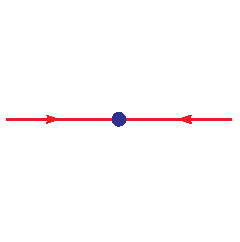
\includegraphics{room1.pdf}\qquad
   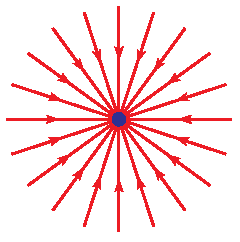
\includegraphics{room2.pdf}\qquad
   \raisebox{0.2\height}{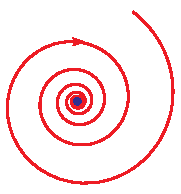
\includegraphics{room3.pdf}}
\end{center}
\end{wfig}

The next few examples illustrate the impact that the``extra room'' 
in dimensions greater than one has on limits.

\begin{eg}\label{ex LIMtwodB}
As a second example, we consider
$\lim\limits_{(x,y)\rightarrow (0,0)}\frac{x^2y}{x^2+y^2}$.
In this example, both the numerator, $x^2y$, and the denominator, 
$x^2+y^2$, tend to zero as $(x,y)$ approaches $(0,0)$, so we have to be more
careful.

 A good way to see the behaviour of a function $f(x,y)$
when $(x,y)$ is close to $(0,0)$ is to switch to the polar coordinates,
$r,\theta$, that are defined by
\begin{align*}
  \\
\hskip1in x&=r\cos\theta\hskip1in
  \smash{\raisebox{-0.6\height}{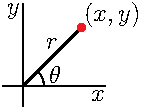
\includegraphics{polar.pdf}}} \\
y&=r\sin\theta \\
\end{align*}
The points $(x,y)$ that are close to $(0,0)$ are those with small $r$,
regardless of what $\theta$ is.
Recall that $\lim\limits_{{(x,y)\rightarrow (0,0)}} f(x,y)=L$ when
$f(x,y)$ approaches $L$ as $(x,y)$ approaches $(0,0)$.
Substituting $x=r\cos\theta$, $y=r\sin\theta$ into that statement turns it into
the statement that $\lim\limits_{{(x,y)\rightarrow (0,0)}} f(x,y)=L$ when
$f(r\cos\theta,r\sin\theta)$ approaches $L$ as $r$ approaches $0$.
For our current example
\begin{align*}
\frac{x^2y}{x^2+y^2}
=\frac{(r\cos\theta)^2(r\sin\theta)}{r^2}
=r\cos^2\theta\sin\theta
\end{align*}
As $\big|r\cos^2\theta\sin\theta\big|\le r$ tends to $0$ as $r$ tends to $0$
(regardless of what $\theta$ does as $r$ tends to $0$) we have
$$
\lim\limits_{(x,y)\rightarrow (0,0)}\frac{x^2y}{x^2+y^2}=0
$$ 
\end{eg}

\begin{eg}\label{ex LIMtwodC}
As a third example, we consider
$\lim\limits_{(x,y)\rightarrow (0,0)}\frac{x^2-y^2}{x^2+y^2}$.
Once again, the best way to see the behaviour of 
$f(x,y)=\frac{x^2-y^2}{x^2+y^2}$ for $(x,y)$ close to $(0,0)$ is to 
switch to polar coordinates.
$$
f(x,y)=\frac{x^2-y^2}{x^2+y^2}=\frac{(r\cos\theta)^2-(r\sin\theta)^2}{r^2}
  =\cos^2\theta-\sin^2\theta
  =\cos(2\theta)
$$
Note that, this time, $f$ is independent of $r$ but does depend on $\theta$.
Here is a greatly magnified sketch of a number of level curves for $f(x,y)$.
\begin{efig}
\begin{center}
   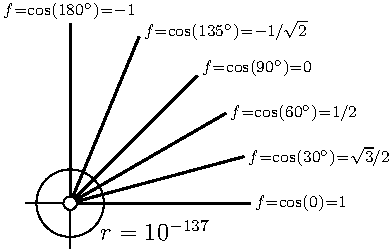
\includegraphics{polarD.pdf}
\end{center}
\end{efig}
Observe that
\begin{itemize}
\item[$\circ$] as $(x,y)$ approaches $(0,0)$ along the ray with 
$2\theta =30^\circ$, $f(x,y)$ approaches the value $\frac{\sqrt{3}}{2}$ 
(and in fact $f(x,y)$ takes the value $\cos(30^\circ)=\frac{\sqrt{3}}{2}$ 
at every point of that ray)
\item[$\circ$] as $(x,y)$ approaches $(0,0)$ along the ray with 
$2\theta =60^\circ$, $f(x,y)$ approaches the value $\frac{1}{2}$ 
(and in fact $f(x,y)$ takes the value $\cos(60^\circ)=\frac{1}{2}$ 
at every point of that ray)
\item[$\circ$] as $(x,y)$ approaches $(0,0)$ along the ray with 
$2\theta =90^\circ$, $f(x,y)$ approaches the value $0$ 
(and in fact $f(x,y)$ takes the value $\cos(90^\circ)=0$ 
at every point of that ray)
\item[$\circ$] and so on
\end{itemize}
So there is not single number $L$ such that $f(x,y)$ approaches
$L$ as $r=|(x,y)|\rightarrow 0$, no matter what the direction of 
approach is. The limit 
$\lim\limits_{(x,y)\rightarrow (0,0)}\frac{x^2-y^2}{x^2+y^2}$
does not exist.


Here is another way to come to the same conclusion.
Pick any really small positive number, like for example 
$10^{-137}$.  For every number $F$ between $-1$ and $1$, like
for example $F=\frac{\sqrt{3}}{2}$, $f(x,y)$ takes the value $F$
for some $(x,y)$ obeying $|(x,y)|<10^{-137}$. That is true regardless
of which really small number you picked. So $f(x,y)=\frac{x^2-y^2}{x^2+y^2}$ 
does not approach any single value as $r=|(x,y)|$ approaches $0$
and we conclude that 
$\lim\limits_{(x,y)\rightarrow (0,0)}\frac{x^2-y^2}{x^2+y^2}$
does not exist.


\end{eg}

\subsection{Optional --- A Nasty Limit That Doesn't Exist}
\begin{eg}\label{eg nasty limit}
In this example we study the behaviour of the function
$$
f(x,y)=\begin{cases}
      \frac{(2x-y)^2}{x-y} & \text{if $x\ne y$}\\[0.05in]
                  0 & \text{if $x=y$}
        \end{cases}
$$ 
as $(x,y)\rightarrow (0,0)$.
Here is a graph of the level curve, $f(x,y)=-3$, for this function.
\begin{efig}
\begin{center}
   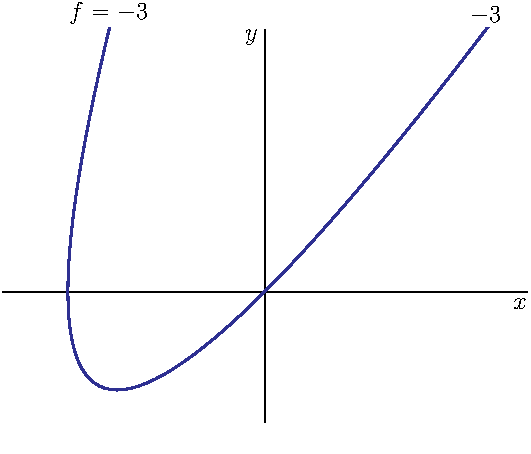
\includegraphics[scale=0.8]{noLimS.pdf}
\end{center}
\end{efig}
Here is a larger graph of level curves, $f(x,y)=c$, for 
various values of the constant $c$.
\begin{efig}
\begin{center}
   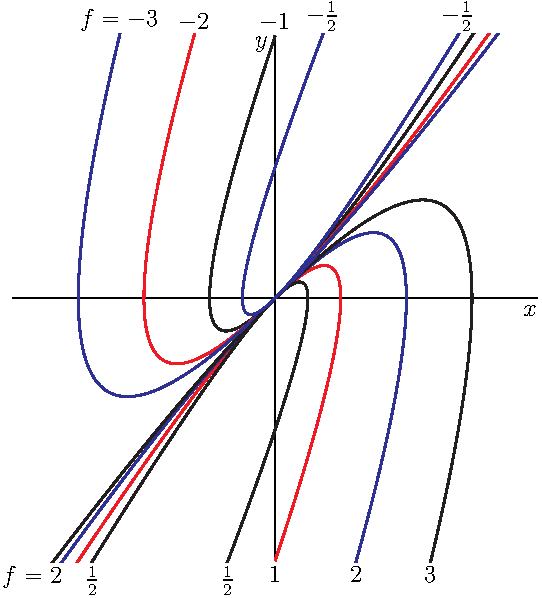
\includegraphics[scale=0.8]{noLim.pdf}
\end{center}
\end{efig}
As before, it helps to convert to polar coordinates --- it is a good 
approach\footnote{Not just a pun.}.
In polar coordinates
$$
f(r\cos\theta,r\sin\theta)
=\begin{cases}
             r\frac{(2\cos\theta-\sin\theta)^2}{\cos\theta-\sin\theta} & 
               \text{if $\cos\theta\ne\sin\theta$}\\[0.05in]
                  0 & \text{if $\cos\theta=\sin\theta$}
 \end{cases}
$$ 
If we approach the origin along any fixed ray $\theta=\text{const}$, 
then $f(r\cos\theta,r\sin\theta)$ is the constant 
$\frac{(2\cos\theta-\sin\theta)^2}{\cos\theta-\sin\theta}$ 
(or $0$ if $\cos\theta=\sin\theta$) times $r$ and so approaches zero as 
$r$ approaches zero. You can see this in the figure below, which shows 
the level curves again, with the rays $\theta=\frac{1}{8}\pi$  
and $\theta=\frac{3}{16}\pi$ superimposed. 
\vadjust{
\begin{efig}
\begin{center}
   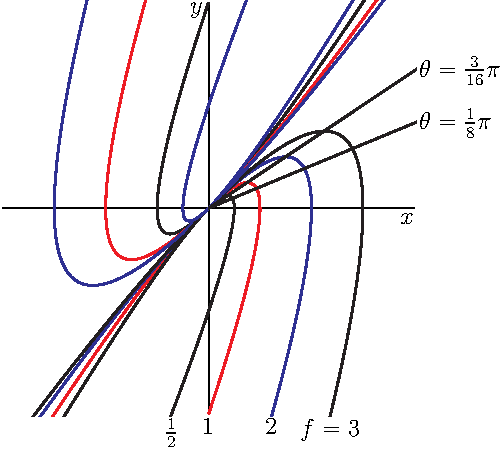
\includegraphics[scale=0.8]{noLimA.pdf}
\end{center}
\end{efig}
}
If you move towards the origin on either of those rays, you first cross 
the $f=3$ level curve, then the $f=2$ level curve, then the $f=1$ level curve, then the $f=\frac{1}{2}$ level curve, and so on.


That $f(x,y)\rightarrow 0$ as $(x,y)\rightarrow (0,0)$ along any fixed ray
is suggestive, but \emph{does not imply} that the limit exists and is zero.
Recall that to have $\lim_{(x,y)\rightarrow(0,0)}f(x,y)=0$,
we need $f(x,y)\rightarrow 0$ no matter how $(x,y)\rightarrow (0,0)$.
It is not sufficient to check only straight line approaches.


In fact, the limit of $f(x,y)$ as $(x,y)\rightarrow (0,0)$ does not exist. 
A good way to see this is to observe that if you fix any $r>0$, 
no matter how small, $f(x,y)$
takes all values from $-\infty$ to $+\infty$ on the circle $x^2+y^2=r^2$.
You can see this in the figure below, which shows the level 
curves yet again, with a circle $x^2+y^2=r^2$ superimposed. 
For every single $-\infty < c <\infty$, the level curve $f(x,y)=c$ crosses
the circle.
\vadjust{
\begin{efig}
\begin{center}
   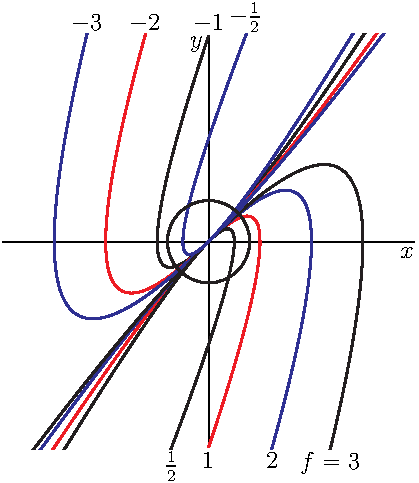
\includegraphics[scale=0.8]{noLimB.pdf}
\end{center}
\end{efig}
}
Consequently there is no one number $L$ such that $f(x,y)$ is close to $L$
whenever $(x,y)$ is sufficiently close to $(0,0)$. The limit 
$\lim_{(x,y)\rightarrow(0,0)} f(x,y)$ does not exist.


Another way to see that  $f(x,y)$ does not have any limit 
as $(x,y)\rightarrow (0,0)$ is to show that $f(x,y)$ does not have  a limit
as $(x,y)$ approaches $(0,0)$ along some specific curve. This can be done
by picking a curve  that makes the denominator,
$x-y$, tend to zero very quickly. One such curve is $x-y=x^3$ or, equivalently,
$y=x-x^3$.  Along this
curve, for $x\ne 0$,
\begin{align*}
f(x,x-x^3)&=\frac{{(2x-x+x^3)}^2}{x-x+x^3}
=\frac{{(x+x^3)}^2}{x^3} \\
&=\frac{{(1+x^2)}^2}{x}\longrightarrow
\begin{cases}+\infty & \text{as $x\rightarrow 0$ with $x>0$}\\
        \noalign{\vskip0.1in}
       -\infty & \text{as $x\rightarrow 0$ with $x<0$}
\end{cases}
\end{align*}
%The figure below shows the level curves, magnified, with the curve $y=x-x^3$ superimposed.
%\vadjust{
%\begin{efig}
%\begin{center}
%   \includegraphics[scale=0.8]{noLimD.pdf}
%\end{center}
%\end{efig}
%}
The choice of the specific power $x^3$ is not important. Any power
$x^p$ with $p>2$ will have the same effect. 

If we send $(x,y)$ to  $(0,0)$ 
along the curve  $x-y=ax^2$ or, equivalently, $y=x-ax^2$, where $a$ is a
nonzero constant,
$$
\lim_{x\rightarrow 0}f(x,x-ax^2)
=\lim_{x\rightarrow 0}\frac{{(2x-x+ax^2)}^2}{x-x+ax^2}
=\lim_{x\rightarrow 0}\frac{{(x+ax^2)}^2}{ax^2}
=\lim_{x\rightarrow 0}\frac{{(1+ax)}^2}{a}
=\frac{1}{a}
$$
This limit depends on the choice of the constant $a$. Once again, this
proves that $f(x,y)$ does not have a limit as $(x,y)\rightarrow (0,0)$.
\end{eg}

%%%%%%%%%%%%%%%%%%%
\section{Partial Derivatives}\label{sec partials}
%%%%%%%%%%%%%%%%%%%
We are now ready to define derivatives of functions of more than one variable.
First, recall how we defined the derivative, $f'(a)$, of a function
of one variable, $f(x)$. We imagined that we were walking along the $x$-axis,
in the positive direction, measuring, for example, the temperature
along the way. We denoted by $f(x)$ the temperature at $x$. The instantaneous rate of change of temperature that we observed as we passed through $x=a$ was
\begin{equation*}
\diff{f}{x}(a) =\lim_{h\rightarrow 0}\frac{f(a+h) - f(a)}{h}
      =\lim_{x\rightarrow a}\frac{f(x) - f(a)}{x-a}
\end{equation*}

Next suppose that we are walking in the $xy$-plane and that the temperature
at $(x,y)$ is $f(x,y)$. We can pass through the point $(x,y)=(a,b)$ moving
in many different directions, and we cannot expect the measured rate of
change of temperature if we walk parallel to the $x$-axis, in the
direction of increasing $x$, to be the same as the measured rate of change of temperature if we walk parallel to the $y$-axis in the direction of increasing $y$. We'll start by considering just those two directions. We'll consider
other directions (like walking parallel to the line $y=x$) later.

Suppose that we are passing through the point $(x,y)=(a,b)$ and that 
we are walking parallel to the $x$-axis (in the positive direction). 
Then our $y$-coordinate will be constant, always taking the value $y=b$. 
So we can think of the measured temperature as the function of one 
variable $B(x) = f(x,b)$ and we will observe the rate of change of temperature 
\begin{equation*}
\diff{B}{x}(a) = \lim_{h\rightarrow 0}\frac{B(a+h) - B(a)}{h}
      = \lim_{h\rightarrow 0}\frac{f(a+h,b) - f(a,b)}{h}
\end{equation*}
This is called the ``partial derivative $f$ with respect to $x$ at $(a,b)$''
and is denoted $\pdiff{f}{x}(a,b)$. Here
\begin{itemize}\itemsep1pt \parskip0pt \parsep0pt
\item[$\circ$] 
the symbol $\partial$, which is read ``partial'', indicates that 
we are dealing with a function of more than one variable, and 
%\item[$\circ$] 
%the subscript $y$ on $\big(\phantom{\pdiff{f}{x}}\big)_y$
%indicates that $y$ is being held fixed, i.e. being treated as a constant, and
\item[$\circ$] 
the $x$ in ${\pdiff{f}{x}}$ indicates that we are differentiating 
with respect to $x$, while $y$ is being held fixed, i.e. being treated as a constant.
\item[$\circ$] 
${\pdiff{f}{x}}$ is read `` partial dee $f$ dee $x$''.
\end{itemize}
Do not write $\diff{}{x}$ when $\pdiff{}{x}$ is appropriate.
We shall later encounter situations when $\diff{}{x}f$ and
$\pdiff{}{x}f$ are both defined and have different meanings.


If, instead, we are passing through the point $(x,y)=(a,b)$ and 
are walking parallel to the $y$-axis (in the positive direction), 
then our $x$-coordinate will be constant, always taking the value $x=a$. 
So we can think of the measured temperature as the function of one 
variable $A(y) = f(a,y)$ and we will observe the rate of change of temperature 
\begin{equation*}
\diff{A}{y}(b) = \lim_{h\rightarrow 0}\frac{A(b+h) - A(b)}{h}
      = \lim_{h\rightarrow 0}\frac{f(a,b+h) - f(a,b)}{h}
\end{equation*}
This is called the ``partial derivative $f$ with respect to $y$ at $(a,b)$''
and is denoted $\pdiff{f}{y}(a,b)$.

Just as was the case for the ordinary derivative $\diff{f}{x}(x)$
(see Definition \eref{CLP100}{def:DIFFderivFunc} in the CLP-1 text),
it is common to treat the partial derivatives of $f(x,y)$ as functions
of $(x,y)$ simply by evaluating the partial derivatives at $(x,y)$ rather 
than at $(a,b)$.
\begin{defn}[Partial Derivatives]\label{def partials}
The $x$- and $y$-partial derivatives of the function $f(x,y)$
are
\begin{align*}
\pdiff{f}{x}(x,y)
  &= \lim_{h\rightarrow 0}\frac{f(x+h,y) - f(x,y)}{h} \\[0.05in]
\pdiff{f}{y}(x,y)
  &= \lim_{h\rightarrow 0}\frac{f(x,y+h) - f(x,y)}{h} 
\end{align*}
respectively. The partial derivatives of functions of more than two variables
are defined analogously.
\end{defn}

Partial derivatives are used a lot. And there many notations for them.
\begin{notn}\label{notn partial}
The partial derivative $\pdiff{f}{x}(x,y)$ of a function $f(x,y)$ is also denoted
\begin{equation*}
\pdiff{f}{x}\qquad
f_x(x,y)\qquad
f_x\qquad
D_xf(x,y)\qquad
D_xf\qquad
D_1 f(x,y)\qquad
D_1 f
\end{equation*}
The subscript $1$ on $D_1 f$ indicates that $f$ is being differentiated with respect to its first variable.
The partial derivative $\pdiff{f}{x}(a,b)$ is also denoted
\begin{equation*}
\pdiff{f}{x}\bigg|_{(a,b)}
\end{equation*}
with the subscript $(a,b)$ indicating that $\pdiff{f}{x}$ is being evaluated
at $(x,y)=(a,b)$.

\medskip
The notation ${\left(\pdiff{f}{x}\right)}_{\!y}$ is used to make explicit
that the variable $y$ is being held.\footnote{There are applications in which there are several variables that cannot be varied independently. For example,
the pressure, volume and temperature of an ideal gas are related by the equation of state $PV= \text{(constant)}T$. In those applications, it may not 
be clear from the context which variables are being held fixed.}

% The abbreviated notation $\pdiff{f}{x}$ for
%${\left(\pdiff{f}{x}\right)}_{\!y}$ is extremely commonly used.
%But it is dangerous to do so, when it is not clear
%from the context, that it is the variable $y$ that is being held fixed.

\end{notn}

\begin{remark}[The Geometric Interpretation of Partial Derivatives]
     \label{rem geom interp}

\ \ \ 
We'll now develop a geometric interpretation of the partial derivative
\begin{equation*}
\pdiff{f}{x}(a,b)  = \lim_{h\rightarrow 0}\frac{f(a+h,b) - f(a,b)}{h}
\end{equation*}
in terms of the shape of the graph $z=f(x,y)$ of the function $f(x,y)$.
That graph appears in the figure below. It looks like the part of
a deformed sphere that is in the first octant. 

The definition of $\pdiff{f}{x}(a,b)$ concerns 
only points on the graph that have $y=b$. 
In other words, the curve of intersection of the
surface $z=f(x,y)$ with the plane $y=b$. That is the red curve in the figure.
The two blue vertical line segments in the figure have heights $f(a,b)$ and
$f(a+h,b)$, which are the two numbers in the numerator 
of $\frac{f(a+h,b) - f(a,b)}{h}$. 
\begin{efig}
\begin{center}
   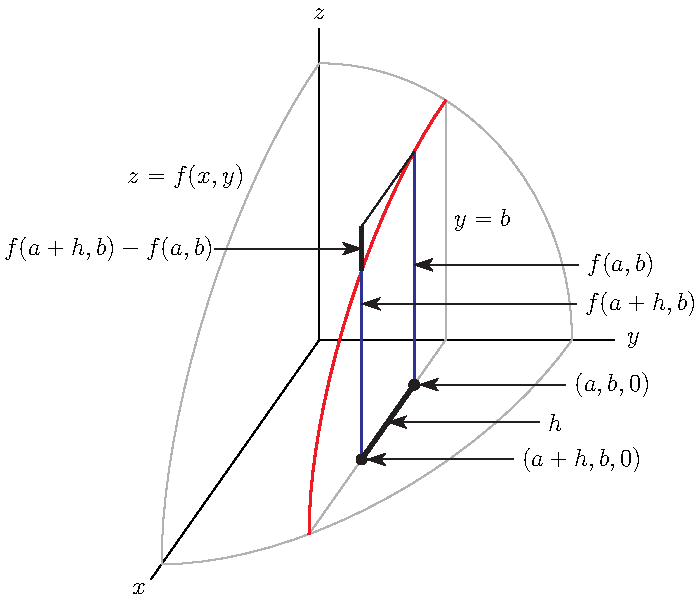
\includegraphics{xderiv.pdf}
\end{center}
\end{efig}
A side view of the curve (looking from the left side of the $y$-axis)
is sketched in the figure below.
\vadjust{
\begin{efig}
\begin{center}
   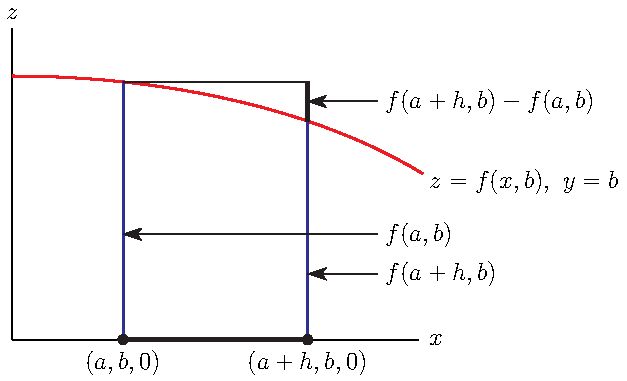
\includegraphics{xderivSide.pdf}
\end{center}
\end{efig}
}
 Again, the two blue vertical line segments 
in the figure have heights $f(a,b)$ and $f(a+h,b)$, which are the two 
numbers in the numerator of $\frac{f(a+h,b) - f(a,b)}{h}$. So
the numerator $f(a+h,b) - f(a,b)$ and denominator $h$ are the rise and run,
respectively, of the curve $z=f(x,b)$ from $x=a$ to $x=a+h$. Thus
$\pdiff{f}{x}(a,b)$ is exactly 
\emph{the slope of (the tangent to) the curve of intersection of the surface 
$z=f(x,y)$ and the plane $y=b$ at the point $\big(a,b, f(a,b)\big)$.}
In the same way
$\pdiff{f}{y}(a,b)$ is exactly 
\emph{the slope of (the tangent to) the curve of intersection of the surface 
$z=f(x,y)$ and the plane $x=a$ at the point $\big(a,b, f(a,b)\big)$.}
\end{remark}

\subsubsection{Evaluation of Partial Derivatives}\label{sec eval partials}
From the above discussion, we see that we can readily compute partial 
derivatives $\pdiff{}{x}$ by using what we already know about ordinary
derivatives $\diff{}{x}$. More precisely, 

\begin{itemize}
\item
to evaluate $\pdiff{f}{x}(x,y)$, treat the $y$ in $f(x,y)$ as a constant
and differentiate the resulting function of $x$ with respect to $x$.
\item
To evaluate $\pdiff{f}{y}(x,y)$, treat the $x$ in $f(x,y)$ as a constant
and differentiate the resulting function of $y$ with respect to $y$.
\item
To evaluate $\pdiff{f}{x}(a,b)$, treat the $y$ in $f(x,y)$ as a constant
and differentiate the resulting function of $x$ with respect to $x$.
Then evaluate the result at $x=a$, $y=b$.
\item
To evaluate $\pdiff{f}{y}(a,b)$, treat the $x$ in $f(x,y)$ as a constant
and differentiate the resulting function of $y$ with respect to $y$.
Then evaluate the result at $x=a$, $y=b$.
\end{itemize}
\noindent
Now for some examples.

\begin{eg}\label{eg partials A}
Let
\begin{equation*}
f(x,y) = x^3+y^2+ 4xy^2 
\end{equation*}
Then, since $\pdiff{}{x}$ treats $y$ as a constant,
\begin{align*}
\pdiff{f}{x}%={\left(\pdiff{f}{x}\right)}_{\!y}
&= \pdiff{}{x}(x^3) + \pdiff{}{x}(y^2) +\pdiff{}{x}(4xy^2) \\
&= 3x^2+0 + 4y^2\pdiff{}{x}(x) \\
&= 3x^2 +4y^2 
\end{align*}
and, since $\pdiff{}{y}$ treats $x$ as a constant,
\begin{align*}
\pdiff{f}{y}%={\left(\pdiff{f}{y}\right)}_{\!x}
&= \pdiff{}{y}(x^3) + \pdiff{}{y}(y^2) +\pdiff{}{y}(4xy^2) \\
&= 0 + 2y + 4x\pdiff{}{y}(y^2) \\
&= 2y+8xy
\end{align*}
In particular, at $(x,y)=(1,0)$ these partial derivatives take the values 
\begin{alignat*}{3}
\pdiff{f}{x}(1,0) &= 3(1)^2 +4(0)^2&=3 \\[0.05in]
\pdiff{f}{y}(1,0) &= 2(0) +8(1)(0)\ &=0 
\end{alignat*}
\end{eg}\goodbreak

\begin{eg}\label{eg partials B}
Let
\begin{equation*}
f(x,y) = y\cos x + xe^{xy}
\end{equation*}
Then, since $\pdiff{}{x}$ treats $y$ as a constant,
$\pdiff{}{x} e^{yx}=y e^{yx}$ and
\begin{align*}
\pdiff{f}{x}(x,y) &= y\pdiff{}{x}(\cos x) + e^{xy}\pdiff{}{x}(x) 
                         +x\pdiff{}{x}\big(e^{xy}\big)
                         \qquad\text{(by the product rule)} \\
                  &= -y\sin x + e^{xy} +xye^{xy} \\[0.05in]
\pdiff{f}{y}(x,y) &= \cos x\pdiff{}{y}(y) + x\pdiff{}{y}\big(e^{xy}\big) \\
                  &= \cos x + x^2e^{xy}
\end{align*}
\end{eg}
Let's move up to a function of four variables. Things generalize
in a quite straight forward way. 
\begin{eg}\label{eg partials C}
Let
\begin{equation*}
f(x,y,z,t) = x\sin(y+2z) +t^2e^{3y}\ln z
\end{equation*}
Then
\begin{align*}
\pdiff{f}{x}(x,y,z,t) &= \sin(y+2z)  \\[0.05in]
\pdiff{f}{y}(x,y,z,t) &= x\cos(y+2z) +3t^2e^{3y}\ln z \\[0.05in]
\pdiff{f}{z}(x,y,z,t) &= 2x\cos(y+2z) +t^2e^{3y}/z \\[0.05in]
\pdiff{f}{t}(x,y,z,t) &= 2te^{3y}\ln z 
\end{align*}
\end{eg}
Now here is a more complicated example --- our function takes a special
value at $(0,0)$. To compute derivatives there we have to revert to
the definition.
\begin{eg}\label{eg partials D}
Set
\begin{equation*}
f(x,y)=\begin{cases}
             \frac{\cos x-\cos y}{x-y}&\text{if $x\ne y$}\\ 
                    0&\text{if $x=y$}
        \end{cases}
\end{equation*}
If $b\ne a$, then for all $(x,y)$ sufficiently close to $(a,b)$,
$f(x,y) = \frac{\cos x-\cos y}{x-y}$ and we can compute the 
partial derivatives of $f$ at $(a,b)$ using the familiar rules of
differentiation. However that is not the case for $(a,b)=(0,0)$. 
To evaluate $f_x(0,0)$, we need to set $y=0$ and find the derivative of
\begin{equation*}
f(x,0) = \begin{cases}
             \frac{\cos x-1}{x}&\text{if $x\ne 0$}\\ 
                    0&\text{if $x=0$}
        \end{cases}
\end{equation*}
with respect to $x$ at $x=0$. To do so, we basically have to apply the
definition
\begin{align*}
f_x(0,0) &= \lim_{h\rightarrow 0}\frac{f(h,0)-f(0,0)}{h} \\
         &= \lim_{h\rightarrow 0}\frac{\frac{\cos h-1}{h}-0}{h}
         &\qquad\text{(Recall that $h\ne 0$ in the limit.)} \\
         &= \lim_{h\rightarrow 0}\frac{\cos h-1}{h^2} \\
         &= \lim_{h\rightarrow 0}\frac{-\sin h}{2h} 
         &\qquad\text{(By l'H\^opital's rule.)} \\
         &= \lim_{h\rightarrow 0}\frac{-\cos h}{2} 
         &\qquad\text{(By l'H\^opital again.)} \\
         &=-\frac{1}{2}
\end{align*}
We could also evaluate the limit of $\frac{\cos h-1}{h^2} $
by substituting in the Taylor expansion 
\begin{equation*}
\cos h = 1 -\frac{h^2}{2}+\frac{h^4}{4!} -\cdots
\end{equation*}

\end{eg}


\begin{eg}\label{eg partials DD}
Again set
\begin{equation*}
f(x,y)=\begin{cases}
             \frac{\cos x-\cos y}{x-y}&\text{if $x\ne y$}\\ 
                    0&\text{if $x=y$}
        \end{cases}
\end{equation*}
We'll now compute $f_y(x,y)$ for all $(x,y)$.

\medskip
\noindent
\emph{The case $y\ne x$:\ \ \ }
When $y\ne x$,
\begin{align*}
f_y(x,y) & = \pdiff{}{y}\frac{\cos x-\cos y}{x-y} \\
         &=\frac{(x-y)\pdiff{}{y}(\cos x-\cos y)
                  - (\cos x-\cos y)\pdiff{}{y}(x-y) }{(x-y)^2} 
       \quad\text{by the quotient rule} \\
         &=\frac{(x-y)\sin y
                  + \cos x-\cos y }{(x-y)^2} 
\end{align*}

\medskip
\noindent
\emph{The case $y= x$:\ \ \ }
When $y = x$,
\begin{align*}
f_y(x,y) &= \lim_{h\rightarrow 0}\frac{f(x,y+h)-f(x,y)}{h}
          = \lim_{h\rightarrow 0}\frac{f(x,x+h)-f(x,x)}{h}
          \hidewidth \\
         &= \lim_{h\rightarrow 0}\frac{\frac{\cos x-\cos(x+h)}{x-(x+h)}-0}{h}
         &\qquad\text{(Recall that $h\ne 0$ in the limit.)} \\
         &= \lim_{h\rightarrow 0}\frac{\cos(x+h)-\cos x}{h^2} 
\end{align*}
Now we apply L'H\^opital's rule twice, remembering that, in this limit,
$x$ is a constant and $h$ is the variable --- so we differentiate with respect to $h$.
\begin{align*}
f_y(x,y)  &= \lim_{h\rightarrow 0}\frac{-\sin(x+h)}{2h}  \\
         &= \lim_{h\rightarrow 0}\frac{-\cos(x+h)}{2}  \\
         &=-\frac{\cos x}{2}
\end{align*}

\medskip
\noindent
\emph{The conclusion:\ \ \ }
\begin{equation*}
f_y(x,y)=\begin{cases}
             \frac{(x-y)\sin y
                  + \cos x-\cos y }{(x-y)^2}&\text{if $x\ne y$}\\ 
                    -\frac{\cos x}{2}&\text{if $x=y$}
        \end{cases}
\end{equation*}
\end{eg}
\begin{eg}[Optional --- A Little Weirdness]\label{eg partials DDD}
In this example, we will see that the function
\begin{equation*}
f(x,y)=\begin{cases}
             \frac{x^2}{x-y}&\text{if $x\ne y$}\\ 
                    0&\text{if $x=y$}
        \end{cases}
\end{equation*}
is \emph{not} continuous at $(0,0)$ and yet has both partial derivatives 
$f_x(0,0)$ and $f_y(0,0)$ perfectly well defined. We'll also see how that is possible. First let's compute the partial derivatives. By definition,
\begin{align*}
f_x(0,0)&=\lim_{h\rightarrow 0}\frac{f(0+h,0)-f(0,0)}{h}
         =\lim_{h\rightarrow 0}\frac{\overbrace{\tfrac{h^2}{h-0}}^{h}-\,0}{h}
         =\lim_{h\rightarrow 0}1 \\
         &=1 \\
f_y(0,0)&=\lim_{h\rightarrow 0}\frac{f(0,0+h)-f(0,0)}{h}
         =\lim_{h\rightarrow 0}\frac{\frac{0^2}{0-h}-0}{h}
         =\lim_{h\rightarrow 0}0 \\
         &=0 
\end{align*}
So the first order partial derivatives $f_x(0,0)$ and $f_y(0,0)$ are perfectly well defined.

To see that, nonetheless, $f(x,y)$ is not continuous at $(0,0)$, we take the limit of $f(x,y)$ as $(x,y)$ approaches $(0,0)$ along the curve $y=x-x^3$.
The limit is
\begin{align*}
\lim_{x\rightarrow 0} f\big(x,x-x^3\big)
=\lim_{x\rightarrow 0} \frac{x^2}{x-(x-x^3)}
=\lim_{x\rightarrow 0} \frac{1}{x}
\end{align*}
which does not exist. Indeed as $x$ approoaches $0$ through positive numbers,
$\frac{1}{x}$ approaches $+\infty$, and as $x$ approoaches $0$ through negative 
numbers, $\frac{1}{x}$ approaches $-\infty$.

So how is this possible? The answer is that $f_x(0,0)$ only involves values of $f(x,y)$ with $y=0$. As $f(x,0)=x$, for all values of $x$, we have that
$f(x,0)$ is a continuous, and indeed a differentiable, function. Similarly, 
$f_y(0,0)$ only involves values of $f(x,y)$ with $x=0$. As $f(0,y)=0$, for all values of $y$, we have that $f(0,y)$ is a continuous, and indeed a 
differentiable, function. On the other hand, the bad behaviour of $f(x,y)$ for $(x,y)$ near
$(0,0)$ only happens for $x$ and $y$ both nonzero.

\end{eg}
Our next example uses implicit differentiation.
\begin{eg}\label{eg partials E}
The equation 
\begin{equation*}
z^5 + y^2 e^z +e^{2x}=0
\end{equation*}
implicitly determines $z$ as a function of $x$ and $y$. 
That is, the function $z(x,y)$ obeys
\begin{equation*}
z(x,y)^5 + y^2 e^{z(x,y)} +e^{2x}=0
\end{equation*}
For example, when $x=y=0$, the equation reduces to
\begin{equation*}
z(0,0)^5=-1
\end{equation*}
which forces\footnote{The only real number $z$ which obeys $z^5=-1$
is $z=-1$. However there are four other complex numbers which also obey
$z^5=-1$.} $z(0,0)=-1$. Let's find the partial derivative $\pdiff{z}{x}(0,0)$.

We are not going to be able to explicitly solve the equation for $z(x,y)$.
All we know is that
\begin{equation*}
z(x,y)^5 + y^2 e^{z(x,y)} + e^{2x} =0
\end{equation*}
for all $x$ and $y$. We can turn this into an equation for $\pdiff{z}{x}(0,0)$
by differentiating\footnote{You should have already seen this technique,
called implicit differentiation, in your first Calculus course. It is covered 
in Section 2.11 in the CLP-1 text.} the whole equation with respect to $x$, 
giving
\begin{equation*}
5z(x,y)^4\ \pdiff{z}{x}(x,y) + y^2 e^{z(x,y)}\ \pdiff{z}{x}(x,y) +2e^{2x}  =0
\end{equation*}
and then setting $x=y=0$, giving
\begin{equation*}
5z(0,0)^4\ \pdiff{z}{x}(0,0) +2  =0
\end{equation*}
As we already know that $z(0,0)=-1$,
\begin{equation*}
\pdiff{z}{x}(0,0) = -\frac{2}{5z(0,0)^4} =-\frac{2}{5}
\end{equation*}
\end{eg}
Next we have a partial derivative disguised as a limit.

\begin{eg}\label{eg partials F}
In this example we are going to evaluate the limit
\begin{equation*}
\lim_{z\rightarrow 0}\frac{(x+y+z)^3-(x+y)^3}{(x+y)z}
\end{equation*} 
The critical observation is that, in taking the limit $z\rightarrow 0$,
$x$ and $y$ are fixed. They do not change as $z$ is getting smaller and
smaller. Furthermore this limit is exactly of the form of the limits
in the Definition \ref{def partials} of partial derivative, disguised by some
obfuscating changes of notation. 

Set
\begin{equation*}
f(x,y,z) = \frac{(x+y+z)^3}{(x+y)}
\end{equation*}
Then
\begin{align*}
\lim_{z\rightarrow 0}\frac{(x+y+z)^3-(x+y)^3}{(x+y)z}
&=\lim_{z\rightarrow 0}\frac{f(x,y,z)-f(x,y,0)}{z}
=\lim_{h\rightarrow 0}\frac{f(x,y,0+h)-f(x,y,0)}{h} \\
&=\pdiff{f}{z}(x,y,0) \\
&={\left[\pdiff{}{z}\frac{(x+y+z)^3}{x+y}\right]}_{z=0} 
\end{align*}
Recalling that $\pdiff{}{z}$ treats $x$ and $y$ as constants, 
we are evaluating the derivative of a function of the form
$\frac{({\rm const}+z)^3}{\rm const}$. So
\begin{align*}
\lim_{z\rightarrow 0}\frac{(x+y+z)^3-(x+y)^3}{(x+y)z}
&={\left.3\frac{(x+y+z)^2}{x+y}\right|}_{z=0} \\
&=3(x+y)
\end{align*}

\end{eg}

The next example highlights a potentially dangerous difference between
ordinary and partial derivatives.

\begin{eg}\label{eg partials G}
In this example we are going to see that, in contrast to the ordinary 
derivative case, $\pdiff{r}{x}$ is not, in general, the same as 
$\big(\pdiff{x}{r}\big)^{-1}$.

Recall that Cartesian and polar coordinates (for $(x,y)\ne (0,0)$ and $r>0$)
are related by
\begin{align*}
\hskip1in x&=r\cos\theta\hskip1in
  \smash{\raisebox{-1.0\height}{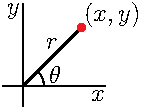
\includegraphics{polar.pdf}}} \\
y&=r\sin\theta \\
r&=\sqrt{x^2+y^2} \\
\tan\theta&=\frac{y}{x}
\end{align*}
We will use the functions 
\begin{equation*}
x(r,\theta) = r\cos\theta\qquad
\text{and}\qquad
r(x,y) = \sqrt{x^2+y^2}
\end{equation*}
Fix any point $(x_0,y_0)\ne (0,0)$ and let
$(r_0,\theta_0)$, $0\le\theta_0<2\pi$, be the corresponding polar coordinates. 
Then
\begin{align*}
\pdiff{x}{r}(r,\theta) = \cos\theta\qquad
\pdiff{r}{x}(x,y) = \frac{x}{\sqrt{x^2+y^2}}
\end{align*}
so that
\begin{align*}
\pdiff{x}{r}(r_0,\theta_0)=\left(\pdiff{r}{x}(x_0,y_0)\right)^{-1}
&\iff \cos\theta_0= \bigg(\frac{x_0}{\sqrt{x_0^2+y_0^2}}\bigg)^{-1}
                  = \left(\cos\theta_0\right)^{-1} \\
&\iff \cos^2\theta_0= 1 \\
&\iff \theta_0=0,\pi
\end{align*}


We can also see pictorially why this happens.
By definition, the partial derivatives
\begin{align*}
\pdiff{x}{r}(r_0,\theta_0)
  &= \lim_{\dee{r}\rightarrow 0}
         \frac{x(r_0+\dee{r},\theta_0) - x(r_0,\theta_0)}{\dee{r}} \\
\pdiff{r}{x}(x_0,y_0)
  &= \lim_{\dee{x}\rightarrow 0}
         \frac{r(x_0+\dee{x},y_0) - r(x_0,y_0)}{\dee{x}} 
\end{align*}
Here we have just renamed the $h$ of Definition \ref{def partials}
to $\dee{r}$ and to $\dee{x}$ in the two definitions.

In computing $\pdiff{x}{r}(r_0,\theta_0)$, $\theta_0$ is held
fixed, $r$ is changed by a small amount $\dee{r}$ and the resulting 
$\dee{x}=x(r_0+\dee{r},\theta_0) - x(r_0,\theta_0)$ is computed.
In the figure on the left below, $\dee{r}$ is the length of the orange
line segment and $\dee{x}$ is the length of the blue line segment.
\begin{efig}
\begin{center}
   \includegraphics{dxdrdrdx1}\qquad\qquad
   \includegraphics{dxdrdrdx2}\qquad
\end{center}
\end{efig}
On the other hand, in computing $\pdiff{r}{x}$, $y$ is held fixed, 
$x$ is changed by a small amount $\dee{x}$ and the resulting 
$\dee{r}=r(x_0+\dee{x},y_0) - r(x_0,y_0)$  is computed. In the figure on 
the right above, $\dee{x}$ is the length of the pink line segment and
$\dee{r}$ is the length of the orange line segment.

Here are the two figures combined together. We have arranged that the same
$\dee{r}$ is used in both computations. In order for the $\dee{r}$'s to 
be the same in both computations, the two $\dee{x}$'s have to be different 
(unless $\theta_0=0,\pi$). So, in general, 
$\pdiff{x}{r}(r_0,\theta_0)\ne \big(\pdiff{r}{x}(x_0,y_0)\big)^{-1}$.
\begin{efig}
\begin{center}
   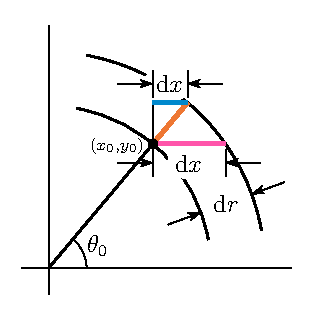
\includegraphics{dxdrdrdx3}
\end{center}
\end{efig}
\end{eg}

\begin{eg}[Optional --- Example \ref{eg partials G}, continued]\label{eg partials GG}
The inverse function theorem, for functions of one variable, says that,
if $y(x)$ and $x(y)$ are inverse functions, meaning that $y\big(x(y)\big)=y$
and $x\big(y(x)\big)=x$, and are differentiable with $\diff{y}{x}\ne 0$, then
\begin{equation*}
\diff{x}{y}(y) = \frac{1}{\diff{y}{x}\big(x(y)\big)}
\end{equation*}
To see this, just apply $\diff{}{y}$ to both sides of $y\big(x(y)\big)=y$
to get $\diff{y}{x}\big(x(y)\big)\ \diff{x}{y}(y)=1$, by the chain rule
(see Theorem \eref{CLP100}{thm:DIFFchainRuleV2} in the CLP-1 text).
In the CLP-1 text, we used this to compute the derivatives of the logarithm 
(see Theorem \eref{CLP100}{thm diff log} in the CLP-1 text) and 
of the inverse trig functions (see Theorem \eref{CLP100}{thm:DIFFinvtrigderiv}
in the CLP-1 text).

We have just seen, in Example \ref{eg partials G}, that we can't be too naive in extending the single variable inverse function theorem to functions of two (or more) variables. On the other hand, there is such an extension, which we will now illustrate, using Cartesian and polar coordinates. For simplicity, we'll restrict our attention to $x>0$, $y>0$, or equivalently, $r>0$, $0<\theta<\frac{\pi}{2}$.
The functions which convert between Cartesian and polar coordinates are
\begin{alignat*}{3}
x(r,\theta)&=r\cos\theta\qquad&
                   r(x,y)&=\sqrt{x^2+y^2} 
\qquad\qquad\smash{\raisebox{-0.63\height}{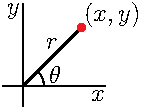
\includegraphics{polar.pdf}}}\\
y(r,\theta)&=r\sin\theta&
                  \theta(x,y)&=\arctan\left(\frac{y}{x}\right)
\end{alignat*}
The two functions on the left convert from polar to Cartesian coordinates and the two functions on the right convert from Cartesian to polar coordinates.
The inverse function theorem (for functions of two variables) says that,
\begin{itemize}\itemsep0pt \parskip0pt \parsep0pt
\item
if you form the first order partial derivatives of the left hand functions
into the matrix
\begin{equation*}
\left[\begin{matrix}
      \pdiff{x}{r}(r,\theta) & \pdiff{x}{\theta}(r,\theta) \\[0.05in]
      \pdiff{y}{r}(r,\theta) & \pdiff{y}{\theta}(r,\theta) 
      \end{matrix}\right]
=\left[\begin{matrix}
      \cos\theta & -r\sin\theta \\[0.05in]
      \sin\theta &  r\cos\theta 
      \end{matrix}\right]
\end{equation*}
\item
and you form the first order partial derivatives of the right hand functions
into the matrix
\begin{equation*}
\left[\begin{matrix}
      \pdiff{r}{x}(x,y) & \pdiff{r}{y}(x,y) \\[0.05in]
      \pdiff{\theta}{x}(x,y) & \pdiff{\theta}{y}(x,y) 
      \end{matrix}\right]
=\left[\begin{matrix}
      \frac{x}{\sqrt{x^2+y^2}} & \frac{y}{\sqrt{x^2+y^2}} \\[0.1in]
      \frac{-\frac{y}{x^2}}{1+(\frac{y}{x})^2} & 
                         \frac{\frac{1}{x}}{1+(\frac{y}{x})^2}
      \end{matrix}\right]
=\left[\begin{matrix}
      \frac{x}{\sqrt{x^2+y^2}} & \frac{y}{\sqrt{x^2+y^2}} \\[0.1in]
      \frac{-y}{x^2+y^2} &  \frac{x}{x^2+y^2}
      \end{matrix}\right]
\end{equation*}
\item
and if you evaluate the second matrix at $x=x(r,\theta)$, $y=y(r,\theta)$,
\begin{equation*}
\left[\begin{matrix}
      \pdiff{r}{x}\big(x(r,\theta),y(r,\theta)\big) & 
                     \pdiff{r}{y}\big(x(r,\theta),y(r,\theta)\big) \\[0.05in]
      \pdiff{\theta}{x}\big(x(r,\theta),y(r,\theta)\big) & 
                      \pdiff{\theta}{y}\big(x(r,\theta),y(r,\theta)\big) 
      \end{matrix}\right]
=\left[\begin{matrix}
      \cos\theta & \sin\theta \\[0.05in]
      -\frac{\sin\theta}{r} & \frac{\cos\theta}{r}
      \end{matrix}\right]
\end{equation*}
\item
and if you multiply\footnote{Matrix multiplication is usually covered in courses on linear algebra, which you may or may not have taken. That's why this example is optional.} the two matrices together
\begin{align*}
&\left[\begin{matrix}
      \pdiff{r}{x}(x,y) & \pdiff{r}{y}(x,y) \\[0.05in]
      \pdiff{\theta}{x}(x,y) & \pdiff{\theta}{y}(x,y) 
      \end{matrix}\right]\ 
\left[\begin{matrix}
      \pdiff{r}{x}\big(x(r,\theta),y(r,\theta)\big) & 
                     \pdiff{r}{y}\big(x(r,\theta),y(r,\theta)\big) \\[0.05in]
      \pdiff{\theta}{x}\big(x(r,\theta),y(r,\theta)\big) & 
                      \pdiff{\theta}{y}\big(x(r,\theta),y(r,\theta)\big) 
      \end{matrix}\right] \\
&\hskip0.5in=\left[\begin{matrix}
      \cos\theta & -r\sin\theta \\[0.05in]
      \sin\theta &  r\cos\theta 
      \end{matrix}\right]\ 
\left[\begin{matrix}
      \cos\theta & \sin\theta \\[0.1in]
      -\frac{\sin\theta}{r} & \frac{\cos\theta}{r}
      \end{matrix}\right]\\
&\hskip0.5in=\left[\begin{matrix}
      (\cos\theta)(\cos\theta) + (-r\sin\theta)(-\frac{\sin\theta}{r})
            &(\cos\theta)(\sin\theta)+(-r\sin\theta)(\frac{\cos\theta}{r}) 
                                                              \\[0.05in]
      (\sin\theta)(\cos\theta)+(r\cos\theta)(-\frac{\sin\theta}{r}) &    
         (\sin\theta)(\sin\theta) + (r\cos\theta)(\frac{\cos\theta}{r})
      \end{matrix}\right]
\end{align*}
\item
then the result is the identity matrix
\begin{equation*}
\left[\begin{matrix}
      1 & 0 \\ 
      0 & 1
      \end{matrix}\right]
\end{equation*}
and indeed it is!

\end{itemize}


\end{eg}

%%%%%%%%%%%%%%%%%%%
\section{Higher Order Derivatives}\label{sec higher order}
%%%%%%%%%%%%%%%%%%%

You have already observed, in your first Calculus course,
that if $f(x)$ is a function of $x$, then its derivative, $\diff{f}{x}(x)$,
is also a function of $x$, and can be differentiated to give the
second order derivative $\difftwo{f}{x}(x)$, which can in turn 
be differentiated yet again to give the third order derivative, 
$f^{(3)}(x)$, and so on.

We can do the same for functions of more than one variable. 
If $f(x,y)$ is a function of $x$ and $y$, then both of its partial
derivatives, $\pdiff{f}{x}(x,y)$ and $\pdiff{f}{y}(x,y)$
are also functions of $x$ and $y$. They can both be differentiated with 
respect to $x$ and they can both be differentiated with respect to $y$. So 
there are four possible second order derivatives. Here they are, together
with various alternate notations.
\begin{alignat*}{5}
\pdiff{}{x}\left(\pdiff{f}{x}\right)(x,y)
   &=\frac{\partial^2 f}{\partial x^2}(x,y) &= f_{xx}(x,y) \\
\pdiff{}{y}\left(\pdiff{f}{x}\right)(x,y)
   &=\frac{\partial^2\ f}{\partial y\partial x}(x,y) &= f_{xy}(x,y) \\
\pdiff{}{x}\left(\pdiff{f}{y}\right)(x,y)
   &=\frac{\partial^2\ f}{\partial x\partial y}(x,y) &= f_{yx}(x,y) \\
\pdiff{}{y}\left(\pdiff{f}{y}\right)(x,y)
   &=\frac{\partial^2 f}{\partial y^2}(x,y) &= f_{yy}(x,y) 
\end{alignat*}
In $\frac{\partial^2\ f}{\partial y\,\partial x}
=\frac{\partial^2}{\partial y\,\partial x}f$, the derivative closest
to $f$, in this case $\pdiff{}{x}$, is applied first.\\
In $f_{xy}$, the derivative with respect to the variable closest
to $f$, in this case $x$, is applied first.
\begin{eg}\label{eg higher order A}
Let $f(x,y) = e^{my}\cos(nx)$. Then
\begin{align*}
f_x &=  -n e^{my}\sin(nx) &
f_y &=   m e^{my}\cos(nx) \\
f_{xx}  &=   -n^2 e^{my}\cos(nx) &
f_{yx} &=   -m n e^{my}\sin(nx) \\
f_{xy}  &=   -m n e^{my}\sin(nx) &
f_{yy} &=   m^2 e^{my}\cos(nx) 
\end{align*}
\end{eg}


\begin{eg}\label{eg higher order B}
Let $f(x,y) = e^{\al x+\be y}$. Then
\begin{align*}
f_x &=  \al e^{\al x+\be y} &
f_y &=  \be e^{\al x+\be y} \\
f_{xx}  &= \al^2  e^{\al x+\be y} &
f_{yx} &=   \be \al e^{\al x+\be y} \\
f_{xy}  &=  \al \be  e^{\al x+\be y} &
f_{yy} &=  \be^2 e^{\al x+\be y}
\end{align*}
More generally, for any integers $m,n\ge 0$,
\begin{equation*}
\frac{\partial^{m+n} f}{\partial x^m\, \partial y^n} 
     = \al^m\be^n e^{\al x+\be y}
\end{equation*}
\end{eg}

\goodbreak
\begin{eg}\label{eg higher order C}
If $f(x_1,x_2,x_3,x_4) = x_1^4\, x_2^3\, x_3^2\, x_4$, then
\begin{align*}
\frac{\partial^4\  f}
          {\partial x_1\, \partial x_2\,\partial x_3\,\partial x_4} 
   &=  \frac{\partial^3 \ }
          {\partial x_1\, \partial x_2\,\partial x_3}
                         \left( x_1^4\, x_2^3\, x_3^2\right)  \\
   &=  \frac{\partial^2 \ }
          {\partial x_1\, \partial x_2}
                         \left( 2\ x_1^4\, x_2^3\, x_3\right)  \\
   &=  \pdiff{}{x_1}
                         \left( 6\ x_1^4\, x_2^2\, x_3\right)  \\
   &=   24\ x_1^3\, x_2^2\, x_3
\end{align*}
and
\begin{align*}
\frac{\partial^4\ f}
          {\partial x_4\, \partial x_3\,\partial x_2\,\partial x_1} 
   &=  \frac{\partial^3 \ }
          {\partial x_4\, \partial x_3\,\partial x_2}
                         \left( 4 x_1^3\, x_2^3\, x_3^2\,x_4\right)  \\
   &=  \frac{\partial^2 \ }
          {\partial x_4\, \partial x_3}
                         \left( 12\ x_1^3\, x_2^2\, x_3^2\,x_4\right)  \\
   &=  \pdiff{}{x_4}
                         \left( 24\ x_1^3\, x_2^2\, x_3\,x_4\right)  \\
   &=   24\ x_1^3\, x_2^2\, x_3
\end{align*}
\end{eg}
Notice that in Example \ref{eg higher order A},
\begin{equation*}
f_{xy}= f_{yx} = -m n e^{my}\sin(nx)
\end{equation*}
and in Example \ref{eg higher order B}
\begin{equation*}
f_{xy}= f_{yx} = \al \be  e^{\al x+\be y} 
\end{equation*}
and in Example \ref{eg higher order C}
\begin{equation*}
\frac{\partial^4\  f}
          {\partial x_1\, \partial x_2\,\partial x_3\,\partial x_4}
= \frac{\partial^4\ f}
          {\partial x_4\, \partial x_3\,\partial x_2\,\partial x_1}  
= 24\ x_1^3\, x_2^2\, x_3
\end{equation*}
In all of these examples, it didn't matter what order we took the derivatives
in. The following theorem\footnote{The history of this important theorem is pretty convoluted. See 
``A note on the history of mixed partial derivatives''
by Thomas James Higgins which was published in 
Scripta Mathematica \textbf{7} (1940), 59-62. } shows that this was no accident.



%%%%%%%%%%%%%%%%%%%%
%\section{The Equality of Mixed Partials}\label{sec mixed partials}
%%%%%%%%%%%%%%%%%%%%

\begin{theorem}[Clairaut's Theorem\footnote{Alexis Clairaut (1713--1765) was a French mathematician, astronomer, and geophysicist.}
%   or Young's Theorem\footnote{William Henry Young (1863--1942) 
%                               was an English mathematician.}
   or Schwarz's Theorem\footnote{Hermann Schwarz (1843--1921) 
                                      was a German mathematician.}]
   \label{thm mixed partials}
If the partial derivatives 
$\frac{\partial^2\hfil f\hfil\,}{\partial x\partial y}$ and 
$\frac{\partial^2\hfil f\hfil\,}{\partial y\partial x}$ exist 
and are continuous at $(x_0,y_0)$, then
$$
\frac{\partial^2\hfil f\hfil\,}{\partial x\partial y}(x_0,y_0)
=\frac{\partial^2\hfil f\hfil\,}{\partial y\partial x}(x_0,y_0)
$$
\end{theorem}

\subsection{Optional --- The Proof of Theorem \ref{thm mixed partials}}
\label{subsec mixed partial proof}

\subsubsection{Outline} 
Here is an outline of the proof of Theorem \ref{thm mixed partials}.
The (numbered) details are in the subsection below.
Fix real numbers $x_0$ and $y_0$ and define 
\begin{equation*}
F(h,k)
=\frac{1}{hk}\big[f(x_0+h,y_0+k)-f(x_0,y_0+k)-f(x_0+h,y_0)+f(x_0,y_0)\big]
\end{equation*}
We define $F(h,k)$ in this way because both partial derivatives
$\frac{\partial^2\hfil f\hfil\,}{\partial x\partial y}(x_0,y_0)$ and
$\frac{\partial^2\hfil f\hfil\,}{\partial y\partial x}(x_0,y_0)$ are  
limits of $F(h,k)$ as $h,k\rightarrow 0$. Precisely, we show in item (1)
in the details below that
\begin{align*}
\pdiff{}{y}
\pdiff{f}{x}(x_0,y_0)
     &= \lim_{k\rightarrow 0}\lim_{h\rightarrow 0}F(h,k) \\
\pdiff{}{x}
\pdiff{f}{y}(x_0,y_0)
&= \lim_{h\rightarrow 0}\lim_{k\rightarrow 0}F(h,k)
\end{align*}
Note that the two right hand sides here are identical except for the 
order in which the limits are taken.

Now, by the mean value theorem (six times),
\begin{align*}
F(h,k)\ &\eqf{(2)}\ \frac{1}{h}
\left[\pdiff{f}{y}(x_0+h,y_0+\theta_1k)
-\pdiff{f}{y}(x_0,y_0+\theta_1k)\right]\cr
\ &\eqf{(3)}\ \pdiff{}{x}
\pdiff{f}{y}(x_0+\theta_2 h,y_0+\theta_1k)\cr
F(h,k)\ &\eqf{(4)}\ \frac{1}{k}
\left[\pdiff{f}{x}(x_0+\theta_3h,y_0+k)
-\pdiff{f}{x}(x_0+\theta_3h,y_0)\right]\cr
\ &\eqf{(5)}\ \pdiff{}{y}
\pdiff{f}{x}(x_0+\theta_3 h,y_0+\theta_4k)\cr
\end{align*}
for some numbers $0<\theta_1,\theta_2,\theta_3,\theta_4<1$.
All of the numbers $\theta_1,\theta_2,\theta_3,\theta_4$ depend 
on $x_0,y_0,h,k$. Hence
\begin{equation*}
\pdiff{}{x}
\pdiff{f}{y}(x_0+\theta_2 h,y_0+\theta_1k)
=\pdiff{}{y}
\pdiff{f}{x}(x_0+\theta_3 h,y_0+\theta_4k)
\end{equation*}
for all $h$ and $k$. Taking the limit $(h,k)\rightarrow(0,0)$ and using
the assumed continuity of both partial derivatives at $(x_0,y_0)$ gives
\begin{equation*}
\lim_{(h,k)\rightarrow (0,0)} F(h,k)
=\pdiff{}{x}
\pdiff{f}{y}(x_0,y_0)
=\pdiff{}{y}
\pdiff{f}{x}(x_0,y_0)
\end{equation*}
as desired. To complete the proof we just have to justify the details
(1), (2), (3), (4) and (5).

\subsubsection{The Details} 
\begin{enumerate}[(1)]
\item
By definition,
\begin{align*}
\pdiff{}{y}
\pdiff{f}{x}(x_0,y_0)
&=\lim_{k\rightarrow 0}\frac{1}{k}
\left[\pdiff{f}{x}(x_0,y_0+k)
-\pdiff{f}{x}(x_0,y_0)\right]\cr
&=\lim_{k\rightarrow 0}\frac{1}{k}
\left[\lim_{h\rightarrow 0}\frac{f(x_0+h,y_0+k)-f(x_0,y_0+k)}{h}
-\lim_{h\rightarrow 0}\frac{f(x_0+h,y_0)-f(x_0,y_0)}{h}\right]\cr
&=\lim_{k\rightarrow 0}\lim_{h\rightarrow 0}
\frac{f(x_0+h,y_0+k)-f(x_0,y_0+k)-f(x_0+h,y_0)+f(x_0,y_0)}{hk}\cr
&= \lim_{k\rightarrow 0}\lim_{h\rightarrow 0}F(h,k)
\end{align*}
Similarly,
\begin{align*}
\pdiff{}{x}
\pdiff{f}{y}(x_0,y_0)
&=\lim_{h\rightarrow 0}\frac{1}{h}
\left[\pdiff{f}{y}(x_0+h,y_0)
-\pdiff{f}{y}(x_0,y_0)\right]\cr
&=\lim_{h\rightarrow 0}\frac{1}{h}
\left[\lim_{k\rightarrow 0}\frac{f(x_0+h,y_0+k)-f(x_0+h,y_0)}{k}
-\lim_{k\rightarrow 0}\frac{f(x_0,y_0+k)-f(x_0,y_0)}{k}\right]\cr
&=\lim_{h\rightarrow 0}\lim_{k\rightarrow 0}
\frac{f(x_0+h,y_0+k)-f(x_0+h,y_0)-f(x_0,y_0+k)+f(x_0,y_0)}{hk}\cr
&= \lim_{h\rightarrow 0}\lim_{k\rightarrow 0}F(h,k)
\end{align*}

\item %2
The mean value theorem (Theorem \eref{CLP100}{thm:DIFFmvt} in the CLP-1 text)
says that, for any differentiable function $\varphi(x)$, 
\begin{itemize}\itemsep0pt \parskip0pt \parsep0pt
\item the slope of the line joining the 
points $\big(x_0,\varphi(x_0)\big)$ and $\big(x_0+k,\varphi(x_0+k)\big)$ on 
the graph of $\varphi$ 
\end{itemize}
is the same as
\begin{itemize}\itemsep0pt \parskip0pt \parsep0pt
\item
the slope of the tangent to the graph 
at some point between $x_0$ and $x_0+k$. 
\end{itemize}
That is, there is some $0<\theta_1<1$ such that
$$
\frac{\varphi(x_0+k)-\varphi(x_0)}{k}=\frac{d\varphi}{dx}(x_0+\theta_1 k)
$$
\begin{efig}
\begin{center}
   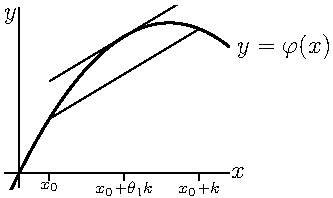
\includegraphics{mvt.pdf}
\end{center}
\end{efig}
Applying this with $x$ replaced by $y$ and $\varphi$ replaced by $G(y)=f(x_0+h,y)-f(x_0,y)$ gives
\begin{align*}
\frac{G(y_0+k)-G(y_0)}{k}
&=\diff{G}{y}(y_0+\theta_1 k)
\qquad\text{for some $0<\theta_1<1$}\cr
&=\pdiff{f}{y}(x_0+h,y_0+\theta_1k)
-\pdiff{f}{y}(x_0,y_0+\theta_1k)
\end{align*}
Hence, for some $0<\theta_1<1$,
\begin{align*}
F(h,k)\ &=\ \frac{1}{h}
\left[\frac{G(y_0+k)-G(y_0)}{k}\right]
=\frac{1}{h}
\left[\pdiff{f}{y}(x_0+h,y_0+\theta_1k)
-\pdiff{f}{y}(x_0,y_0+\theta_1k)\right]
\end{align*}

\item %3
Define $H(x)=\pdiff{f}{y}(x,y_0+\theta_1k)$. By the mean value theorem,
\begin{align*}
F(h,k)\ &=\ \frac{1}{h}\left[H(x_0+h)-H(x_0)\right]\cr
&=\ \diff{H}{x}(x_0+\theta_2 h)
\qquad\text{for some $0<\theta_2<1$}\cr
&=\pdiff{}{x}
\pdiff{f}{y}(x_0+\theta_2 h,y_0+\theta_1k)
\end{align*}

\item %4
Define $A(x)=f(x,y_0+k)-f(x,y_0)$. By the mean value theorem,
\begin{align*}
F(h,k)\ &=\ \frac{1}{k} \left[\frac{A(x_0+h)-A(x_0)}{h}\right] \\
&=\ \frac{1}{k}\diff{A}{x}(x_0+\theta_3 h)
\qquad\text{for some $0<\theta_3<1$} \\
&=\frac{1}{k}
\left[\pdiff{f}{x}(x_0+\theta_3h,y_0+k)
-\pdiff{f}{x}(x_0+\theta_3h,y_0)\right]
\end{align*}

\item %5
Define $B(y)=\pdiff{f}{x}(x_0+\theta_3h,y)$. By the mean value theorem
\begin{align*}
F(h,k)\ &=\ \frac{1}{k}\left[B(y_0+k)-B(y_0)\right] \\
&=\ \diff{B}{y}(y_0+\theta_4 k)
\qquad\text{for some $0<\theta_4<1$} \\
&=\pdiff{}{y}
\pdiff{f}{x}(x_0+\theta_3 h,y_0+\theta_4k)
\end{align*}

\end{enumerate}
This completes the proof of Theorem \ref{thm mixed partials}.

\subsection{Optional --- An Example of 
$\frac{\partial^2\ f}{\partial x\partial y}(x_0,y_0)
\ne\frac{\partial^2\ f}{\partial y\partial x}(x_0,y_0)$}
\label{subsec mixed partials counterexample}

In Theorem \ref{thm mixed partials}, we showed that
$
\frac{\partial^2\hfil f\hfil\,}{\partial x\partial y}(x_0,y_0)
=\frac{\partial^2\hfil f\hfil\,}{\partial y\partial x}(x_0,y_0)
$
\textbf{if} the partial derivatives 
$\frac{\partial^2\hfil f\hfil\,}{\partial x\partial y}$ and 
$\frac{\partial^2\hfil f\hfil\,}{\partial y\partial x}$ exist 
and are continuous at $(x_0,y_0)$. Here is an example which shows that
if the partial derivatives 
$\frac{\partial^2\hfil f\hfil\,}{\partial x\partial y}$ and 
$\frac{\partial^2\hfil f\hfil\,}{\partial y\partial x}$ 
are not continuous at $(x_0,y_0)$, then it is possible that 
$
\frac{\partial^2\hfil f\hfil\,}{\partial x\partial y}(x_0,y_0)
\ne\frac{\partial^2\hfil f\hfil\,}{\partial y\partial x}(x_0,y_0)$.

Define
$$
f(x,y)=\begin{cases}
        xy\frac{x^2-y^2}{x^2+y^2} & \text{if $(x,y)\ne (0,0)$}\\
              0                   & \text{if $(x,y)=(0,0)$}
       \end{cases}
$$
This function is continuous everywhere. Note that $f(x,0)=0$ for all $x$ and
$f(0,y)=0$ for all $y$. We now compute the first order
partial derivatives. For $(x,y)\ne (0,0)$,
\begin{alignat*}{3}
\pdiff{f}{x}(x,y)
  &= y\frac{x^2-y^2}{x^2+y^2} +xy\frac{2x}{x^2+y^2}
      - xy\frac{2x(x^2-y^2)}{{(x^2+y^2)}^2}
  &\ = y\frac{x^2-y^2}{x^2+y^2}  + xy\frac{4xy^2}{{(x^2+y^2)}^2}\cr
\pdiff{f}{y}(x,y)
  &= x\frac{x^2-y^2}{x^2+y^2} -xy\frac{2y}{x^2+y^2}
      - xy\frac{2y(x^2-y^2)}{{(x^2+y^2)}^2}
  &\ = x\frac{x^2-y^2}{x^2+y^2}  - xy\frac{4yx^2}{{(x^2+y^2)}^2}
\end{alignat*}
For $(x,y)= (0,0)$,
\begin{alignat*}{5}
\pdiff{f}{x}(0,0)
  &= \left[\diff{}{x}f(x,0)\right]_{x=0}
  &= \left[\diff{}{x} 0\right]_{x=0}
  &=0\\
\pdiff{f}{y}(0,0)
  &= \left[\diff{}{y}f(0,y)\right]_{y=0}
  &= \left[\diff{}{y} 0\right]_{y=0}
  &=0
\end{alignat*}
By way of summary, the two first order partial derivatives are
\begin{align*}
f_x(x,y)&=\begin{cases}
         y\frac{x^2-y^2}{x^2+y^2}  + \frac{4x^2y^3}{{(x^2+y^2)}^2} 
                                         & \text{if $(x,y)\ne (0,0)$}\\
              0                          & \text{if $(x,y)=(0,0)$}
          \end{cases} \\[0.05in]
f_y(x,y)&=\begin{cases}
          x\frac{x^2-y^2}{x^2+y^2}  - \frac{4x^3y^2}{{(x^2+y^2)}^2} 
                                         & \text{if $(x,y)\ne (0,0)$} \\
              0                          & \text{if $(x,y)=(0,0)$}
           \end{cases}
\end{align*}
Both $\pdiff{f}{x}(x,y)$ and  $\pdiff{f}{y}(x,y)$ are continuous.
Finally, we compute 
\begin{alignat*}{5}
\frac{\partial^2\ f}{\partial x\partial y}(0,0)
&=\left[\diff{}{x} f_y(x,0)\right]_{x=0}
&=\lim_{h\rightarrow 0}\frac{1}{h}\left[f_y(h,0)-f_y(0,0)\right]
&=\lim_{h\rightarrow 0}\frac{1}{h}\left[h\frac{h^2-0^2}{h^2+0^2}-0\right]
&=1
\\[0.05in]
\frac{\partial^2\ f}{\partial y\partial x}(0,0)
&=\left[\diff{}{y} f_x(0,y)\right]_{y=0}
&=\lim_{k\rightarrow 0}\frac{1}{k}\left[f_x(0,k)-f_x(0,0)\right]
&=\lim_{k\rightarrow 0}\frac{1}{k}\left[k\frac{0^2-k^2}{0^2+k^2}-0\right]
&=-1
\end{alignat*}




\section{The Chain Rule}\label{sec chain rule}

You already routinely use the one dimensional chain
rule 
\begin{equation*}
\diff{}{t}f\big(x(t)\big) 
= \diff{f}{x}\big(x(t)\big)\ \diff{x}{t}(t)
\end{equation*}
in doing computations like 
\begin{equation*}
\diff{}{t}\sin(t^2) = \cos(t^2)\ 2t
\end{equation*}
In this example, $f(x)=\sin(x)$ and $x(t)=t^2$.

We now generalize the chain rule to functions of more than one variable.
For concreteness, we concentrate on the case in which all functions 
are functions of two variables. That is, we find the partial derivatives 
$\pdiff{F}{s}$ and $\pdiff{F}{t}$ of a function $F(s,t)$ that is defined
as a composition
\begin{equation*}
  F(s,t)=f\big(x(s,t)\,,\,y(s,t)\big)
\end{equation*}
We are using the name $F$ for the new function $F(s,t)$ as a reminder that
it is closely related to, though not the same as, the function $f(x,y)$.
The partial derivative $\pdiff{F}{s}$ is the rate of change of $F$ when $s$ is varied with $t$ held constant. When $s$ is varied, both the $x$-argument,
$x(s,t)$, and the $y$-argument, $y(s,t)$, in $f\big(x(s,t)\,,\,y(s,t)\big)$
vary. Consequently, the chain rule for $f\big(x(s,t)\,,\,y(s,t)\big)$
is a sum of two terms --- one resulting from the variation
of the $x$-argument and the other resulting from the variation of 
the $y$-argument.

\begin{theorem}[The Chain Rule]\label{thm:chainRule}
Assume that all first order partial derivatives of $f(x,y)$, $x(s,t)$
and $y(s,t)$ exist and are continuous. Then the same is true for $F(s,t)=f\big(x(s,t)\,,\,y(s,t)\big)$ and
\begin{align*}
\pdiff{F}{s}(s,t)
&=  \pdiff{f}{x}\big(x(s,t)\,,\,y(s,t)\big)\, \pdiff{x}{s}(s,t)
   +\pdiff{f}{y}\big(x(s,t)\,,\,y(s,t)\big)\, \pdiff{y}{s}(s,t) \\
\pdiff{F}{t}(s,t)
&=  \pdiff{f}{x}\big(x(s,t)\,,\,y(s,t)\big)\, \pdiff{x}{t}(s,t)
   +\pdiff{f}{y}\big(x(s,t)\,,\,y(s,t)\big)\, \pdiff{y}{t}(s,t) 
\end{align*}
\end{theorem}\noindent
We will give the proof of this theorem in \S\ref{subsec higher d chain rule},
below. It is common to state this chain rule as 
\begin{align*}
\pdiff{F}{s}
&=  \pdiff{f}{x}\, \pdiff{x}{s}
   +\pdiff{f}{y}\, \pdiff{y}{s} \\
\pdiff{F}{t}
&=  \pdiff{f}{x}\, \pdiff{x}{t}
   +\pdiff{f}{y}\, \pdiff{y}{t} 
\end{align*}
That is, it is common to suppress the function arguments. But you 
should make sure that
you understand what the arguments are before doing so.

Theorem \ref{thm:chainRule} is given for the case that $F$ is the
composition of a function of two variables, $f(x,y)$, with two functions, 
$x(s,t)$ and $y(s,t)$,  of two variables each. There is nothing magical about 
the number two. There are obvious variants for any numbers of variables. 
For example,
\begin{impeqn}\label{eqn chain rule A}
if $F(t) = f\big(x(t),y(t),z(t)\big)$, then
\begin{align*}
\diff{F}{t}(t) &= \pdiff{f}{x}\big(x(t)\,,\,y(t)\,,\,z(t)\big)\, \diff{x}{t}(t)
           +\pdiff{f}{y}\big(x(t)\,,\,y(t)\,,\,z(t)\big)\, \diff{y}{t}(t) \\
     &\hskip1in   +\pdiff{f}{z}\big(x(t)\,,\,y(t)\,,\,z(t)\big)\, \diff{z}{t}(t)
\end{align*}

\end{impeqn}
and
\begin{impeqn}\label{eqn chain rule B}
if $F(s,t) = f\big(x(s,t)\big)$, then
\begin{align*}
\pdiff{F}{t}(s,t) &= \diff{f}{x}\big(x(s,t)\big)\, \pdiff{x}{t}(s,t)
\end{align*}

\end{impeqn}

There will be a large number of examples shortly. First, here is a
memory aid.

\subsection{Memory Aids for the Chain Rule}
\label{subsec memory aid}

We recommend strongly that you use the following procedure, without leaving
out any steps, the first couple of dozen times that you use the chain rule.
\begin{description}
\item[Step 1] 
List \textbf{explicitly} all the functions involved and specify the
arguments of each function. Ensure that all different functions have different
names. Invent new names for some of the functions if necessary. In the
case of the chain rule in Theorem  \ref{thm:chainRule}, the list would be
\begin{equation*}
f(x,y)\qquad\qquad
x(s,t)\qquad\qquad
y(s,t)\qquad\qquad
F(s,t)=f\big(x(s,t),y(s,t)\big)
\end{equation*}
While the functions $f$ and $F$ are closely related, they are not the same.
One is a function of $x$ and $y$ while the other is a function of $s$ and
$t$.
\item[Step 2] 
Write down the template
\begin{equation*}
\pdiff{F}{s}=\frac{\partial f}{ }\frac{ }{\partial s}
\end{equation*}
Note that 
\begin{itemize}
\item
The function $F$ appears once in the numerator on the left.
The function $f$, from which $F$ is constructed by a change of variables,
appears once in the numerator on the right.

\item
The variable in the denominator on the left appears once in the
denominator on the right. 
\end{itemize}

\item[Step 3] 
Fill in the blanks with every variable that makes sense. In 
particular, since $f$ is a function of $x$ and $y$, it may only be 
differentiated with respect to $x$ and $y$. So we add together
two copies of our template --- one for $x$ and one for $y$:
\begin{equation*}
\pdiff{F}{s}
=\pdiff{f}{x }\pdiff{x }{s}
+\pdiff{f}{y }\pdiff{y }{s}
\end{equation*}
Note that $x$ and $y$ are functions of $s$ so that the derivatives
$\pdiff{x }{s}$ and $\pdiff{y }{s}$ make sense.
The first term, $\pdiff{f}{x }\pdiff{x }{s}$, arises from the variation
of $x$ with respect to $s$ and the second term, $\pdiff{f}{y }\pdiff{y }{s}$, 
arises from the variation of $y$ with respect to $s$.


\item[Step 4] 
Put in the functional dependence \textbf{explicitly}. Fortunately,
there is only one functional dependence that makes sense. 
The left hand side is a function of $s$ and $t$. Hence the
 right hand side must also be a function of $s$ and $t$. As $f$ is a
 function of $x$ and $y$, this is achieved by evaluating $f$ at $x=x(s,t)$
 and $y=y(s,t)$.
$$
\pdiff{F}{s}(s,t)=
  \pdiff{f}{x}\big(x(s,t),y(s,t)\big)
  \pdiff{x}{s}(s,t)
  +\pdiff{f}{y}\big(x(s,t),y(s,t)\big)
  \pdiff{y}{s}(s,t)
$$
If you fail to put in the arguments, or at least if you fail to remember
what the arguments are, you may forget that $\pdiff{f}{x}$ and $\pdiff{f}{y}$
depend on $s$ and $t$. Then, if you have to compute a second derivative of $F$,
you will probably fail to differentiate the factors  $\pdiff{f}{x}\big(x(s,t),y(s,t)\big)$ and
$\pdiff{f}{y}\big(x(s,t),y(s,t)\big)$.

\end{description}



To help remember the formulae of Theorem \ref{thm:chainRule}, it is sometimes 
also useful to pretend that our variables are physical quantities with 
$f,F$ having units of grams, $x,y$ having units of meters and $s,t$ having units of seconds. Note that
\begin{itemize}
\item 
the left hand side, $\pdiff{F}{s}$, has units grams per second.
\item
Each term on the right hand side
contains the partial derivative of $f$ with respect to a different
 independent variable. That independent variable appears once in the
 denominator and once in the numerator, so that its units (in this case meters)
cancel out. Thus both of the terms $\pdiff{f}{x }\pdiff{x }{s}$
and $\pdiff{f}{y }\pdiff{y }{s}$ on the right hand side also have 
the units grams per second.

\item
Hence both sides of the equation have the same units.

\end{itemize}



Here is a pictorial procedure that uses a \emph{tree diagram} to help remember 
the chain rule
$
\pdiff{}{s}f\big(x(s,t),y(s,t)\big)=
  \pdiff{f}{x}
  \pdiff{x}{s}
  +\pdiff{f}{y}
  \pdiff{y}{s}
$. 
As in the figure on the left below,
\begin{itemize}\itemindent-15pt \itemsep1pt \parskip0pt \parsep0pt
\item[$\circ$]
write, on the top row, ``$f$''.
\item[$\circ$]
Write, on the middle row, each of the variables that the function $f(x,y)$ 
depends on, namely``$x$'' and ``$y$''.
\item[$\circ$]
Write, on the bottom row, 
   \begin{itemize}\itemsep1pt \parskip0pt \parsep0pt
       \item below $x$, each of the variables that the function $x(s,t)$ 
                   depends on, namely ``$s$'' and ``$t$'', and 
       \item below $y$, each of the variables that the function $y(s,t)$ 
                   depends on, namely ``$s$'' and ``$t$''. 
    \end{itemize}
\item[$\circ$]
Draw a line joining each function with each of the variables that it depends 
on.
\item[$\circ$]
Then, as in the figure on the right below, write beside each line, the partial
derivative of the function at the top of the line with respect to the variable at the bottom of the line.
\begin{efig}
\begin{center}
   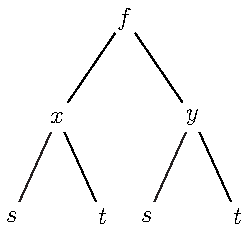
\includegraphics{decTreeA.pdf}\qquad\qquad
   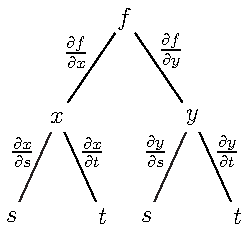
\includegraphics{decTreeB.pdf}
\end{center}
\end{efig}
\item[$\circ$]
Finally
   \begin{itemize}\itemsep1pt \parskip0pt \parsep0pt
       \item observe, from the figure below, that there are two paths
               from $f$, on the top, to $s$, on the bottom. One path goes from
               $f$ at the top, through $x$ in the middle to $s$ at the
               bottom.  The other path goes from
               $f$ at the top, through $y$ in the middle to $s$ at the
               bottom.  
       \item For each such path, multiply together the partial derivatives
               beside the lines of the path. In this example, the two products 
               are $\pdiff{f}{x}\,\pdiff{x}{s}$, for the first path, and
               $\pdiff{f}{y}\,\pdiff{y}{s}$, for the second path.
       \item Then add together those products, giving, in this example,
              $\pdiff{f}{x}\,\pdiff{x}{s}+\pdiff{f}{y}\,\pdiff{y}{s}$.
       \item Put in the arguments, as in Step 4, above.
   \end{itemize}
\item[$\circ$]
   That's it. We have 
\begin{equation*}
\pdiff{}{s}f\big(x(s,t),y(s,t)\big)=
  \pdiff{f}{x}\big(x(s,t),y(s,t)\big)
  \pdiff{x}{s}(s,t)
  +\pdiff{f}{y}\big(x(s,t),y(s,t)\big)
  \pdiff{y}{s}(s,t)
\end{equation*}
\begin{efig}
\begin{center}
   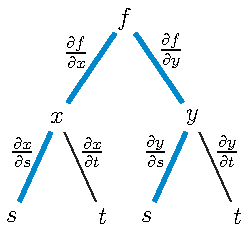
\includegraphics{decTreeS.pdf}
\end{center}
\end{efig}
\end{itemize} 

\begin{eg}\label{eg decTree}
The right hand side of the chain rule
\begin{align*}
\diff{}{t}f\big(x(t)\,,\,y(t)\,,\,z(t)\big) &= \pdiff{f}{x}\big(x(t)\,,\,y(t)\,,\,z(t)\big)\, \diff{x}{t}(t)
           +\pdiff{f}{y}\big(x(t)\,,\,y(t)\,,\,z(t)\big)\, \diff{y}{t}(t) \\
     &\hskip1in   +\pdiff{f}{z}\big(x(t)\,,\,y(t)\,,\,z(t)\big)\, \diff{z}{t}(t)
\end{align*}
of Equation \eqref{eqn chain rule A}, without arguments, is
     $\pdiff{f}{x}\, \diff{x}{t}
     +\pdiff{f}{y}\, \diff{y}{t}
     +\pdiff{f}{z}\, \diff{z}{t}$. 
The corresponding tree diagram is
\begin{efig}
\begin{center}
   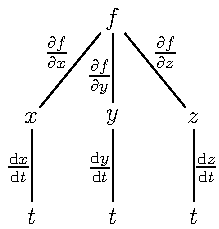
\includegraphics{decTreeTT.pdf}
\end{center}
\end{efig}
Because $x(t)$, $y(t)$ and $z(t)$ are each functions of just one variable, the
derivatives beside the lower lines in the tree are ordinary, rather 
than partial, derivatives. 
\end{eg}

\subsection{Chain Rule Examples}
\label{subsec chain rule examples}

Let's do some routine examples first and work our way to some trickier
ones.


\begin{eg}[$\pdiff{}{s}f\big(x(s,t),y(s,t)\big)$]\label{eg:chainRuleAA}
In this example we find $\pdiff{}{s}f\big(x(s,t),y(s,t)\big)$ for 
\begin{equation*}
f(x,y)=e^{xy}\qquad x(s,t)=s \qquad y(s,t)=\cos t
\end{equation*}
Define $F(s,t)=f\big(x(s,t)\,,\,y(s,t)\big)$. The appropriate chain rule for this 
example is the upper equation of Theorem \ref{thm:chainRule}.
\begin{equation*}
\pdiff{F}{s}(s,t)
=  \pdiff{f}{x}\big(x(s,t)\,,\,y(s,t)\big)\, \pdiff{x}{s}(s,t)
   +\pdiff{f}{y}\big(x(s,t)\,,\,y(s,t)\big)\, \pdiff{y}{s}(s,t)
\end{equation*}
For the given functions
\begin{align*}
f(x,y)&=e^{xy}  \\
\pdiff{f}{x}(x,y)&= ye^{xy}  &
\pdiff{f}{x}\big(x(s,t),y(s,t)\big)&= y(s,t) e^{x(s,t)\,y(s,t)}
                                    = \cos t\ e^{s\cos t} \\
\pdiff{f}{y}(x,y)&= xe^{xy}  &
\pdiff{f}{y}\big(x(s,t),y(s,t)\big)&= x(s,t) e^{x(s,t)\,y(s,t)}
                                    = s\ e^{s\cos t} \\
\pdiff{x}{s}&=1 &
\pdiff{y}{s}&=0  
\end{align*}
so that 
$$
\pdiff{F}{s}(s,t)=\overbrace{\left\{\cos t\ e^{s\cos t}\right\}}^{\pdiff{f}{x}}
                  \overbrace{(1) }^{\pdiff{x}{s}}
                  +\overbrace{\left\{s\ e^{s\cos t}\right\}}^{\pdiff{f}{y}}
                    \overbrace{(0) }^{\pdiff{y}{s}}
                 = \cos t\ e^{s\cos t}
$$

\end{eg}

\begin{eg}[$\diff{}{t}f\big(x(t),y(t)\big)$]\label{eg:chainRuleA}
In this example we find $\diff{}{t}f\big(x(t),y(t)\big)$
for 
\begin{equation*}
f(x,y)=x^2-y^2\qquad x(t)=\cos t \qquad y(t)=\sin t
\end{equation*}

Define $F(t)=f\big(x(t),y(t)\big)$. Since $F(t)$ is a function of one
variable its derivative is denoted $\diff{F}{t}$ rather than $\pdiff{F}{t}$.
The appropriate chain rule for this example (see \eqref{eqn chain rule A}) 
is
$$
\diff{F}{t}(t)=
  \pdiff{f}{x}\big(x(t),y(t)\big) \diff{x}{t}(t)
  +\pdiff{f}{y}\big(x(t),y(t)\big) \diff{y}{t}(t)
$$
For the given functions
\begin{align*}
f(x,y)&=x^2-y^2  \\
\pdiff{f}{x}(x,y)&= 2x  &
\pdiff{f}{x}\big(x(t),y(t)\big)&= \phantom{-}2x(t) =\phantom{-}2\cos t  \\
\pdiff{f}{y}(x,y)&= -2y  &
\pdiff{f}{y}\big(x(t),y(t)\big)&= -2y(t)  =-2\sin t \\
\diff{x}{t}&=-\sin t &
\diff{y}{t}&=\cos t  
\end{align*}
so that 
$$
\diff{F}{t}(t)=(2\cos t)(-\sin t) +(-2\sin t)(\cos t) = -4\sin t\cos t
$$
Of course, in this example we can compute $F(t)$ explicitly
$$
F(t)=f\big(x(t),y(t)\big)=x(t)^2-y(t)^2=\cos^2t-\sin^2t
$$
and then differentiate
$$
F'(t)=2(\cos t)(-\sin t)-2(\sin t)(\cos t) = -4 \sin t\cos t
$$
\end{eg}


\begin{eg}[$\pdiff{}{t}f(x+ct)$]\label{eg:chainRuleB}
 Define
$u(x,t)=x+ct$ and $w(x,t)=f(x+ct)=f\big(u(x,t)\big)$. Then
$$
\pdiff{}{t}f(x+ct)
=\pdiff{w}{t}(x,t)
=\diff{f}{u}\big(u(x,t)\big)  \pdiff{u}{t}(x,t)
=c\, f'(x+ct)
$$
\end{eg}

\goodbreak
\begin{eg}[$\frac{\partial^2\hfill}{\partial t^2}f(x+ct)$]\label{eg:chainRuleC}
 Define  $w(x,t)=f(x+ct)$ and 
$W(x,t)=\pdiff{w}{t}(x,t)=cf'(x+ct)=F\big(u(x,t)\big)$ 
where $F(u)=cf'(u)$ and $u(x,t)=x+ct$. Then
$$
\frac{\partial^2\hfill}{\partial t^2}f(x+ct)
=\pdiff{W}{t}(x,t)
=\diff{F}{u}\big(u(x,t)\big)  \pdiff{u}{t}(x,t)
=c\,f''(x+ct)\,c
=c^2\,f''(x+ct)
$$
\end{eg}

\begin{eg}[Equation of state]\label{eg:chainRuleD} 
Suppose that we are told that $F(P,V,T)=0$ and 
that we are to find  $\pdiff{P}{T}$.

Before we can find $\pdiff{P}{T}$, we first have to decide what it means.
This happens regularly in applications. In fact, this particular problem
comes from thermodynamics. The variables $P,\ V,\ T$ are the pressure,
volume and temperature, respectively, of some gas. These three variables
are not independent. They are related by an equation of state, here denoted
$F(P,V,T)=0$. Given values for any two of $P,\ V,\ T$, the third can be
found by solving $F(P,V,T)=0$. We are being asked to find 
$\pdiff{P}{T}$. This implicitly instructs us to treat
$P$, in this problem, as the dependent variable. So a careful wording of
this problem (which you will never encounter in the ``real world'') would
be the following. The function $P(V,T)$ is defined by $F\big(P(V,T),V,T)=0$.
Find $\big(\pdiff{P}{T}\big)_V$. That is, find the rate of change of
pressure as the temperature is varied, while holding the volume fixed.

Since we are not told explicitly what $F$ is, we cannot solve explicitly
for $P(V,T)$. So, instead we differentiate both sides of 
$$
F\big(P(V,T),V,T\big)=0
$$
with respect to $T$, while holding $V$ fixed. Think of the left hand side,
$F\big(P(V,T),V,T\big)$, as being $F\big(P(V,T),Q(V,T),R(V,T)\big)$
with $Q(V,T)=V$ and $R(V,T)=T$. By the chain rule,
$$
\pdiff{}{T}F\big(P(V,T),Q(V,T),R(V,T)\big)
=F_1\pdiff{P}{T}
+F_2\pdiff{Q}{T}
+F_3\pdiff{R}{T}=0
$$
with $F_j$ referring to the partial derivative of $F$ with respect to its
$j^{\rm th}$ argument.
Experienced chain rule users never introduce $Q$ and $R$. Instead, 
they just write
$$
\pdiff{F}{P}\pdiff{P}{T}
+\pdiff{F}{V}\pdiff{V}{T}
+\pdiff{F}{T}\pdiff{T}{T}=0
$$
Recalling that $V$ and $T$ are the independent variables and that, in computing
$\pdiff{}{T}$, $V$ is to be treated as a constant,
$$
\pdiff{V}{T}=0\qquad\qquad \pdiff{T}{T} = 1
$$
Now putting in the functional dependence
$$
\pdiff{F}{P}\big(P(V,T),V,T\big)
\pdiff{P}{T}(V,T)
+\pdiff{F}{T}\big(P(V,T),V,T\big)=0
$$
and solving
$$
\pdiff{P}{T}(V,T)
=-\frac{\pdiff{F}{T}\big(P(V,T),V,T\big)}
{\pdiff{F}{P}\big(P(V,T),V,T\big)}
$$
\end{eg}

\begin{eg}\label{eg:chainRuleE} 
Suppose that $f(x,y)=0$ and that we are to find $\difftwo{y}{x}$.
\smallskip

Once again, $x$ and $y$ are not independent variables. Given a value for
either $x$ or $y$, the other is determined by solving $f(x,y)=0$. Since
we are asked to find $\difftwo{y}{x}$, it is $y$ that is to be viewed
as a function of $x$, rather than the other way around. So $f(x,y)=0$ really
means that, in this problem, $f\big(x,y(x)\big)=0$ for all $x$. 
Differentiating both sides of this equation with respect to $x$,
\begin{align*}
&\phantom{\implies a} f\big(x,y(x)\big) = 0\qquad\text{for all }x\\
&\implies \diff{}{x}f\big(x,y(x)\big) = 0
\end{align*}

Note that $\diff{}{x}f\big(x,y(x)\big)$ is not the same as
$f_x\big(x,y(x)\big)$. The former is, by definition, the rate of change with 
respect to $x$ of $g(x)=f\big(x,y(x)\big)$. Precisely,
\begin{align}
\diff{g}{x}&=\lim_{\De x\rightarrow 0}\frac{g(x+\De x)-g(x)}{\De x}\notag\\
&=\lim_{\De x\rightarrow 0}\frac{f\big(x+\De x\,,\,y(x+\De x)\big)
-f\big(x\,,\,y(x)\big)}{\De x}
\tag{$*$}
\end{align}
On the other hand, by definition,
\begin{align}
f_x(x,y)&=\lim_{\De x\rightarrow 0}\frac{f(x+\De x,y)-f(x,y)}{\De x}\notag\\
\implies f_x\big(x,y(x)\big)
&=\lim_{\De x\rightarrow 0}\frac{f\big(x+\De x\,,\,y(x)\big)
                              -f\big(x\,,\,y(x)\big)}
{\De x}
\tag{$**$}
\end{align}
The right hand sides of $(*)$ and $(**)$ are not the same. 
In $\diff{g}{x}$, as $\De x$ varies the value of $y$ that is substituted 
into the  first $f(\cdots)$ on the right hand side, namely $y(x+\De x)$, 
changes as $\De x$ changes. That is, we are computing the rate of change 
of $f$ along the (curved) path $y=y(x)$.
 In $(**)$, the corresponding value of $y$ is $y(x)$ and is independent of 
$\De x$. That is, we are computing the rate of change of $f$ along a 
horizontal straight line. As a concrete example,
suppose that $f(x,y)=x+y$. Then, $0=f\big(x\,,\,y(x)\big)=x+y(x)$ gives
$y(x)=-x$ so that
\begin{equation*}
\diff{}{x}f\big(x,y(x)\big)
=\diff{}{x}f(x,-x)
=\diff{}{x}[x+(-x)]
=\diff{}{x}0 =0
\end{equation*}
But $f(x,y)=x+y$ implies that $f_x(x,y)=1$ for all $x$ and $y$ so that
\begin{equation*}
f_x(x,y(x))=f_x(x,y)\Big|_{y=-x}=1\Big|_{y=-x}=1
\end{equation*}

Now back to 
\begin{align}
&\phantom{\implies a} f\big(x,y(x)\big) = 0\qquad\text{for all }x\notag\\
\hskip.5in&\implies \diff{}{x}f\big(x,y(x)\big) = 0\notag\\
&\implies f_x\big(x,y(x)\big)\diff{x}{x}
+f_y\big(x,y(x)\big)\diff{y}{x}(x) = 0\qquad\text{by the chain rule}\notag\\
&\implies 
\diff{y}{x}(x) = -\frac{f_x\big(x,y(x)\big)}{f_y\big(x,y(x)\big)}\notag\\
&\implies 
\difftwo{y }{x}(x) = -\diff{}{x}\left[\frac{f_x\big(x,y(x)\big)}{f_y\big(x,y(x)\big)}\right]\notag\\
&\phantom{\implies a \difftwo{y }{x}(x)}= -\frac{f_y\big(x,y(x)\big)\diff{}{x}[f_x\big(x,y(x)\big)]
-f_x\big(x,y(x)\big)\diff{}{x}[f_y\big(x,y(x)\big)]}
{f_y\big(x,y(x)\big)^2}
\tag{$\dagger$}
\end{align}
by the quotient rule. Now it suffices to substitute in
 $\diff{}{x}\big[f_x\big(x,y(x)\big)\big]$ and 
$\diff{}{x}\big[f_y\big(x,y(x)\big)\big]$. For the former apply
the chain rule to $h(x) = u\big(x,y(x)\big)$ with $u(x,y)=f_x\big(x,y\big)$.
\begin{align*}
\diff{}{x}\big[f_x\big(x,y(x)\big)\big]&=\diff{h}{x}(x)\cr
&=u_x\big(x,y(x)\big)\diff{x}{x}
+u_y\big(x,y(x)\big)\diff{y}{x}(x)\cr
&=f_{xx}\big(x,y(x)\big)\diff{x}{x}
+f_{xy}\big(x,y(x)\big)\diff{y}{x}(x)\cr
&=f_{xx}\big(x,y(x)\big)
-f_{xy}\big(x,y(x)\big)
\left[\frac{f_x\big(x,y(x)\big)}{f_y\big(x,y(x)\big)}\right]
\end{align*}
Substituting this and 
\begin{align*}
\diff{}{x}\big[f_y\big(x,y(x)\big)\big]
&=f_{yx}\big(x,y(x)\big)\diff{x}{x}
+f_{yy}\big(x,y(x)\big)\diff{y}{x}(x)\cr
&=f_{yx}\big(x,y(x)\big)
-f_{yy}\big(x,y(x)\big)
\left[\frac{f_x\big(x,y(x)\big)}{f_y\big(x,y(x)\big)}\right]
\end{align*}
into the right hand side of $(\dagger)$ gives the final answer.
\begin{align*}
\difftwo{y}{x}(x) 
= -\frac{
                                 f_y f_{xx}
                             -  f_y f_{xy} \frac{f_x}{f_y}
                             - f_x f_{yx}
                             + f_x f_{yy}\frac{f_x}{f_y}}
                         {f_y^2}
= -\frac{
                                 f_y^2 f_{xx}
                             - 2 f_x f_y f_{xy}
                               + f_x^2 f_{yy}}
                         {f_y^3}
\end{align*}
with all of $f_x$, $f_y$, $f_{xx}$, $f_{xy}$, $f_{yy}$ having arguments
$\big(x\,,\,y(x)\big)$. 

\end{eg}

We now move on to the proof of Theorem \ref{thm:chainRule}.
To give you an idea of how the proof will go, we first review
the proof of the familiar one dimensional chain rule. 

\subsection{Review of the Proof of 
     $\diff{}{t}f\big(x(t)\big)  = \diff{f}{x}\big(x(t)\big)\ \diff{x}{t}(t)$}
\label{subsec 1d chain rule}


As a warm up, let's review the proof of the one dimensional chain rule
\begin{equation*}
    \diff{}{t}f\big(x(t)\big) = \diff{f}{x}\big(x(t)\big)\ \diff{x}{t}(t)
\end{equation*}
assuming that $\diff{x}{t}$ exists and that $\diff{f}{x}$ is continuous.
We wish to find the derivative of $F(t) = f\big(x(t)\big)$.
By definition
\begin{align*}
F'(t) &= \lim_{h\rightarrow 0}\frac{F(t+h)-F(t)}{h} \\
      &= \lim_{h\rightarrow 0}\frac{f\big(x(t+h)\big)-f\big(x(t)\big)}{h}
\end{align*}
Notice that the numerator is the difference of $f(x)$ evaluated at two nearby
values of $x$, namely $x_1=x(t+h)$ and $x_0=x(t)$. The mean value theorem is
a good tool for studying the difference in the values of $f(x)$ at two
nearby points. Recall that the mean value theorem says that, for any 
given $x_0$ and  $x_1$, there exists an (in general unknown) $c$ between 
them so that
\begin{equation*}
f(x_1) - f(x_0) = f'(c)\ (x_1-x_0)
\end{equation*}
For this proof, we choose $x_0=x(t)$ and $x_1=x(t+h)$. The the mean value theorem tells us that there exists a $c_h$ so that
\begin{align*}
f\big(x(t+h)\big)-f\big(x(t)\big)
&= f(x_1)-f(x_0)
 = f'(c_h)\ \big[x(t+h)-x(t)\big]
\end{align*}
We have put the subscript $h$ on $c_h$ to emphasise that
$c_h$, which is between $x_0=x(t)$ and $x_1=x(t+h)$, may depend on $h$.
Now since  $c_h$ is trapped between $x(t)$ and $x(t+h)$ and since
$x(t+h)\rightarrow x(t)$ as $h\rightarrow 0$, we have that $c_h$ must 
also tend to $x(t)$ as $h\rightarrow 0$. Plugging this into the definition of $F'(t)$,
\begin{align*}
F'(t)  &= \lim_{h\rightarrow 0}\frac{f\big(x(t+h)\big)-f\big(x(t)\big)}{h} \\
&= \lim_{h\rightarrow 0}\frac{f'(c_h)\ \big[x(t+h)-x(t)\big]}{h} \\
&= \lim_{h\rightarrow 0}f'(c_h)\ 
    \lim_{h\rightarrow 0}\frac{x(t+h)-x(t)}{h} \\
&= f'\big(x(t)\big)\ x'(t)
\end{align*}
as desired.

\subsection{Proof of Theorem \ref{thm:chainRule}}
\label{subsec higher d chain rule}

We'll now prove the formula for $\pdiff{}{s} f\big( x(s,t)\,,\,y(s,t)\big)$
that is given in Theorem \ref{thm:chainRule}. The proof uses the same ideas 
as the proof of the one variable chain rule, that we have just reviewed.

We wish to find the partial derivative with respect to $s$ of
$F(s,t)=f\big(x(s,t)\,,\,y(s,t)\big)$. By definition
\begin{align*}
\pdiff{F}{s}(s,t)
&=\lim_{h\rightarrow 0}\frac{F(s+h,t)-F(s,t)}{h}  \\
&=\lim_{h\rightarrow 0}\frac{f\big(x(s+h,t)\,,\,y(s+h,t)\big)
                       -f\big(x(s,t)\,,\,y(s,t)\big)}{h} 
\end{align*}
The numerator is the difference of $f(x,y)$ evaluated at two nearby
values of $(x,y)$, namely $(x_1,y_1)=\big(x(s+h,t)\,,\,y(s+h,t)\big)$ and 
$(x_0,y_0)=\big(x(s,t)\,,\,y(s,t)\big)$. In going from $(x_0,y_0)$
to $(x_1,y_1)$, both the $x$ and $y$-coordinates change. By adding
and subtracting we can separate the change in the $x$-coordinate from the
change in the $y$-coordinate.
\begin{align*}
f(x_1,y_1) - f(x_0,y_0)
=\big\{f(x_1,y_1) - f(x_0,y_1)\big\}  + \big\{f(x_0,y_1) - f(x_0,y_0)\big\}
\end{align*} 
The first half, $\big\{f(x_1,y_1) - f(x_0,y_1)\big\}$, has the same $y$ argument
in both terms and so is the difference of the 
function of one variable $g(x) = f(x,y_1)$ (viewing $y_1$ just as a constant)
evaluated at the two nearby values, $x_0$, $x_1$, of $x$. Consequently, 
we can make use of the mean value theorem as we did in 
\S\ref{subsec 1d chain rule} above. 
There is a $c_{x,h}$ between $x_0=x(s,t)$ and $x_1=x(s+h,t)$ such that
\begin{align*}
f(x_1,y_1) - f(x_0,y_1)
&=g(x_1) - g(x_0)
=g'(c_{x,h}) [x_1-x_0] 
=\pdiff{f}{x}(c_{x,h},y_1)\,[x_1-x_0] \\
&=\pdiff{f}{x}\big(c_{x,h}\,,\,y(s+h,t)\big)\,\big[x(s+h,t)-x(s,t)\big]
\end{align*}
We have introduced the two subscripts in $c_{x,h}$ to remind ourselves that
it may depend on $h$ and that it lies between the two $x$-values
$x_0$ and $x_1$.

Similarly, the second half, $\big\{f(x_0,y_1) - f(x_0,y_0)\big\}$, 
is the difference of the function of one variable  $h(y) = f(x_0,y)$ 
(viewing $x_0$ just as a constant)
evaluated at the two nearby values, $y_0$, $y_1$, of $y$. So, by the mean
value theorem,
\begin{align*}
f(x_0,y_1) - f(x_0,y_0)
&=h(y_1) - h(y_0)
=h'(c_{y,h}) [y_1-y_0]
=\pdiff{f}{y}(x_0,c_{y,h})\,[y_1-y_0] \\
&=\pdiff{f}{y}\big(x(s,t)\,,\,c_{y,h}\big)\,\big[y(s+h,t)-y(s,t)\big] 
\end{align*}
for some (unknown) $c_{y,h}$ between $y_0=y(s,t)$ and $y_1=y(s+h,t)$.
Again, the two subscripts in $c_{y,h}$ remind ourselves that
it may depend on $h$ and that it lies between the two $y$-values
$y_0$ and $y_1$.
So, noting that, as $h$ tends to zero, $c_{x,h}$, which is trapped
between $x(s,t)$ and $x(s+h,t)$, must tend to $x(s,t)$, and
$c_{y,h}$, which is trapped between $y(s,t)$ and $y(s+h,t)$, must tend to $y(s,t)$,
\begin{align*}
\pdiff{F}{s}(s,t))  
&= \lim_{h\rightarrow 0}\frac{f\big(x(s+h,t)\,,\,y(s+h,t)\big)
                       -f\big(x(s,t)\,,\,y(s,t)\big)}{h} \\
&= \lim_{h\rightarrow 0}\frac{
      \pdiff{f}{x}\big(c_{x,h}\,,\,y(s+h,t)\big)\,\big[x(s+h,t)-x(s,t)\big]
       }{h} \\
&\hskip0.75in+ \lim_{h\rightarrow 0}\frac{
      \pdiff{f}{y}\big(x(s,t)\,,\,c_{y,h}\big)\,\big[y(s+h,t)-y(s,t)\big] }{h} \\
&= \lim_{h\rightarrow 0}
      \pdiff{f}{x}\big(c_{x,h}\,,\,y(s+h,t)\big)\ 
    \lim_{h\rightarrow 0}\frac{x(s+h,t)-x(s,t)}{h} \\
&\hskip0.75in+ \lim_{h\rightarrow 0}
      \pdiff{f}{y}\big(x(s,t)\,,\,c_{y,h}\big)
     \lim_{h\rightarrow 0}\frac{y(s+h,t)-y(s,t) }{h} \\
&=  \pdiff{f}{x}\big(x(s,t)\,,\,y(s,t)\big)\, \pdiff{x}{s}(s,t)
   +\pdiff{f}{y}\big(x(s,t)\,,\,y(s,t)\big)\, \pdiff{y}{s}(s,t)
\end{align*}
We can of course follow the same procedure to evaluate the partial derivative 
with respect to $t$. This concludes the proof of Theorem \ref{thm:chainRule}.





%%%%%%%%%%%%%%%%%%%
\section{Tangent Planes and Normal Lines}\label{sec tangent planes}
%%%%%%%%%%%%%%%%%%%

The tangent line to the curve $y=f(x)$ at the point $\big(x_0,f(x_0)\big)$ 
is the straight line that fits the curve best\footnote{It is possible,
but beyond the scope of this text, to give a precise meaning to
``fits best''.} 
at that point.
Finding tangent lines was probably one of the first applications 
of derivatives that you saw. See, for example, 
Theorem \eref{CLP100}{thm:DIFFtangentLine} in the CLP-1 text.
The analog of the tangent line one dimension up is the tangent plane.
The tangent plane to a surface $S$ at a point  $(x_0,y_0,z_0)$ is the plane
that fits $S$ best at $(x_0,y_0,z_0)$. For example, the tangent plane
to the hemisphere 
\begin{equation*}
S=\Set{(x,y,z)}{x^2+y^2+(z-1)^2=1,\ 0\le z\le 1}
\end{equation*} 
at the origin is the $xy$-plane, $z=0$.
\begin{efig}
\begin{center}
   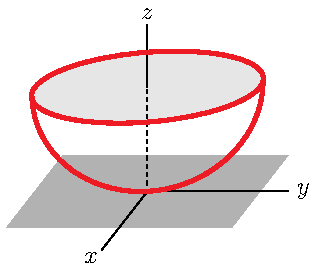
\includegraphics{sphereTanPlane.pdf}
\end{center}
\end{efig}


We are now going to determine, as our first application of partial derivatives,
the tangent plane to a general surface $S$ at a general point $(x_0,y_0,z_0)$
lying on the surface.
We will also determine the line which passes through $(x_0,y_0,z_0)$ 
and whose direction is perpendicular to $S$ at $(x_0,y_0,z_0)$. It is called
the normal line to $S$ at $(x_0,y_0,z_0)$. 

For example, the following 
figure shows the side view of the tangent plane (in black) and normal line 
(in blue) to the surface $z=x^2+y^2$ (in red) at the point $(0,1,1)$.
\begin{efig}
\begin{center}
   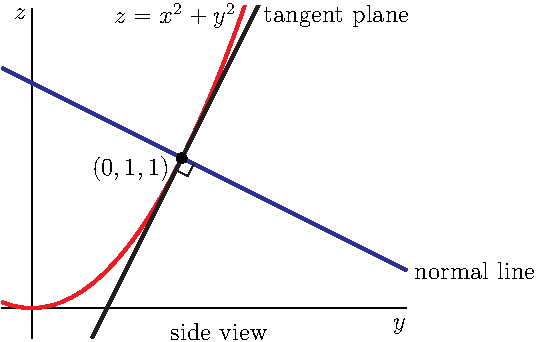
\includegraphics{tanPlaneNormalLine.pdf}
\end{center}
\end{efig}

 Recall, from \eqref{eqn of plane}, that to specify any plane, we need
\begin{itemize}\itemsep1pt \parskip0pt \parsep0pt
\item[$\circ$] 
one point on the plane and
\item[$\circ$] 
a vector perpendicular to the plane, i.e. a normal vector,
\end{itemize}
and recall, from \eqref{par eqn of line}, that to specify any line, we need
\begin{itemize}\itemsep1pt \parskip0pt \parsep0pt
\item[$\circ$] 
one point on the line and
\item[$\circ$] 
a direction vector for the line.
\end{itemize}
We already have one point that is on both the tangent plane of interest 
and the normal line of interest --- namely $\big(x_0,y_0,z_0\big)$. 
Furthermore we can use any (nonzero) vector that is perpendicular to $S$
at $(x_0,y_0,z_0)$ as both the normal vector to the tangent plane and the
direction vector of the normal line.

So our main task is to determine a normal vector to the surface $S$ at $(x_0,y_0,z_0)$. That's what we do now, first for surfaces of the
form $z=f(x,y)$ and then, more generally, for surfaces of the form 
$G(x,y,z)=0$.

%%%%
\subsection{Surfaces of the Form $z=f(x,y)$.}
%%%%
We construct a vector perpendicular to the surface $z=f(x,y)$ at
$\big(x_0\,,\,y_0\,,\,f(x_0,y_0)\big)$
by, first, constructing two tangent vectors to the specified surface at 
the specified point, and, second, taking the cross product
of those two tangent vectors. Consider the red curve in the figure
below. It is the intersection of our surface $z=f(x,y)$
\vadjust{
\begin{efig}
\begin{center}
   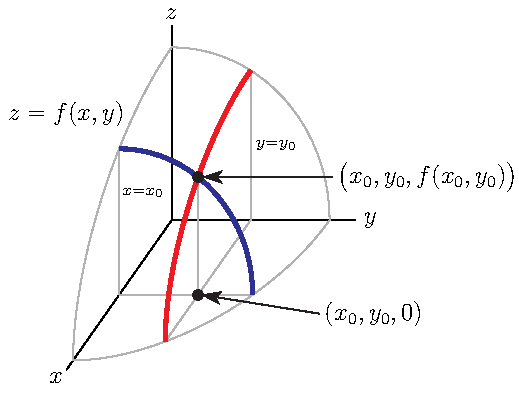
\includegraphics{tanPlaneAA.pdf}\qquad\qquad
   %\raisebox{0.3\height}{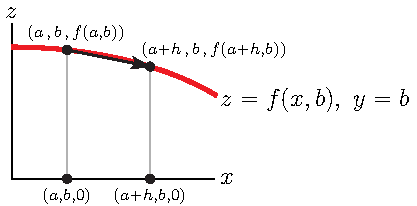
\includegraphics{tanPlaneAside.pdf}}
\end{center}
\end{efig}
}
with the plane $y=y_0$. Here is a side view of the red curve. 
\vadjust{
\begin{efig}
\begin{center}
%   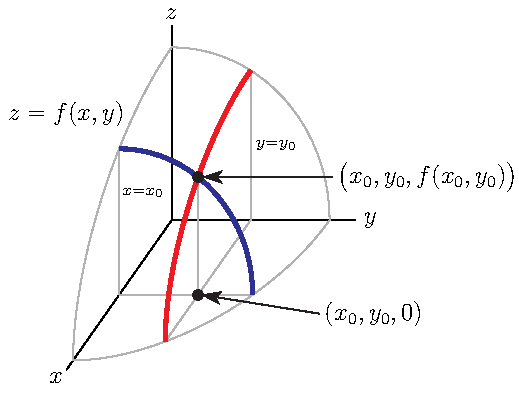
\includegraphics{tanPlaneAA.pdf}\qquad\qquad
%   \raisebox{0.3\height}{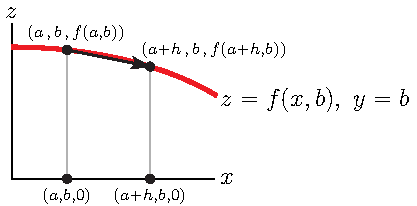
\includegraphics{tanPlaneAside.pdf}}
   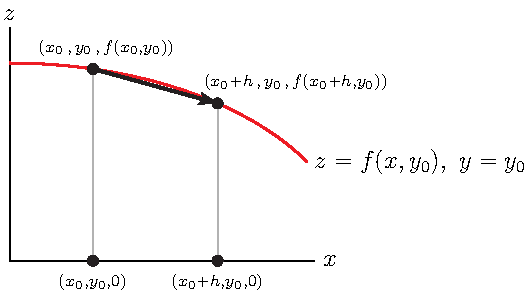
\includegraphics{tanPlaneAAside.pdf}
\end{center}
\end{efig}
}
The vector from the point $\big(x_0\,,\,y_0\,,\,f(x_0,y_0)\big)$, on the
red curve, to the point $\big(x_0+h\,,\,y_0\,,\,f(x_0+h,y_0)\big)$, 
also on the red curve, is almost tangent to the red curve, if 
$h$ is very small. As $h$ tends to $0$, that vector, which is
\begin{equation*}
\llt h\,,\, 0\,,\, f(x_0+h,y_0)-f(x_0,y_0)  \rgt
\end{equation*}
becomes exactly tangent to the curve. However its length also tends
to $0$. If we divide by $h$, and then take the limit $h\rightarrow 0$,
we get
\begin{align*}
\lim_{h\rightarrow 0}\frac{1}{h} 
             \llt h\,,\, 0\,,\, f(x_0+h,y_0)-f(x_0,y_0)  \rgt
&=\lim_{h\rightarrow 0} 
           \llt 1\,,\, 0\,,\, \frac{f(x_0+h,y_0)-f(x_0,y_0)}{h}  \rgt 
\end{align*}
Since the limit $\lim_{h\rightarrow 0} \frac{f(x_0+h,y_0)-f(x_0,y_0)}{h}$
is the definition of the partial derivative $f_x(x_0,y_0)$, we get that
\begin{align*}
\lim_{h\rightarrow 0}\frac{1}{h} 
             \llt h\,,\, 0\,,\, f(x_0+h,y_0)-f(x_0,y_0)  \rgt
&=\llt 1\,,\, 0\,,\, f_x(x_0,y_0)\rgt
\end{align*}
is a nonzero vector that is exactly tangent to the red curve and
hence is also tangent to our surface $z=f(x,y)$ at the point 
$\big(x_0\,,\,y_0\,,\,f(x_0,y_0)\big)$. 

For the second tangent vector, we repeat
the process with the blue curve in the figure at the beginning of this
subsection. That blue curve is the intersection of our surface $z=f(x,y)$ 
with the plane $x=x_0$.
Here is a front view of the blue curve. 
\begin{efig}
\begin{center}
   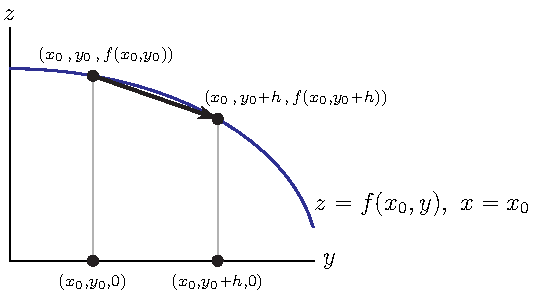
\includegraphics{tanPlaneBBside.pdf}
\end{center}
\end{efig}
When $h$ is very small, the vector 
\begin{equation*}
\frac{1}{h} \llt 0\,,\, h\,,\, f(x_0,y_0+h)-f(x_0,y_0)  \rgt
\end{equation*}
from the point $\big(x_0\,,\,y_0\,,\,f(x_0,y_0)\big)$, on the
blue curve, to $\big(x_0\,,\,y_0+h\,,\,f(x_0,y_0+h)\big)$, 
also on the blue curve, (and lengthened by a factor $\frac{1}{h}$) is 
almost tangent to the blue curve. Taking the limit $h\rightarrow0$ gives the tangent vector
\begin{align*}
\lim_{h\rightarrow 0}\frac{1}{h} 
         \llt 0\,,\, h\,,\, f(x_0,y_0+h)-f(x_0,y_0)  \rgt
&=\lim_{h\rightarrow 0} 
          \llt 0\,,\, 1\,,\, \frac{f(x_0,y_0+h)-f(x_0,y_0)}{h}  \rgt \\
&=\llt 0\,,\, 1\,,\, f_y(x_0,y_0)\rgt
\end{align*}
to the blue curve at the point  $\big(a\,,\,b\,,\,f(a,b)\big)$. 

Now that we have two vectors in the tangent plane to the surface $z=f(x,y)$ 
at $\big(x_0\,,\,y_0\,,\,f(x_0,y_0)\big)$, we can find a normal vector to 
the tangent plane by taking their cross product. Their cross product is
\begin{align*}
\llt 1\,,\, 0\,,\, f_x(x_0,y_0)\rgt\times\llt 0\,,\, 1\,,\, f_y(x_0,y_0)\rgt
&=\det\left[\begin{matrix}\hi& \hj &\hk\\ 
                   1 & 0 & f_x(x_0,y_0)\\ 
                   0 & 1 & f_y(x_0,y_0)\end{matrix}\right] \\[0.05in]
&=-f_x(x_0,y_0)\,\hi - f_y(x_0,y_0)\,\hj +\hk
\end{align*}
and we have that the vector
$$
-f_x(x_0,y_0)\,\hi - f_y(x_0,y_0)\,\hj +\hk
$$
is perpendicular to the surface $z=f(x,y)$ at  $\big(x_0\,,\,y_0\,,\,f(x_0,y_0)\big)$.

The tangent plane to the surface $z=f(x,y)$ at $\big(x_0\,,\,y_0\,,\,f(x_0,y_0)\big)$
is the plane through $\big(x_0\,,\,y_0\,,\,f(x_0,y_0)\big)$ with normal vector
$-f_x(x_0,y_0)\,\hi - f_y(x_0,y_0)\,\hj +\hk$. This plane has equation
\begin{equation*}
-f_x(x_0,y_0)\,(x-x_0) - f_y(x_0,y_0)\,(y-y_0) +\big(z-f(x_0,y_0)\big) =0
\end{equation*}
or, after a little rearrangement,
$$
z = f(x_0,y_0) + f_x(x_0,y_0)\,(x-x_0) + f_y(x_0,y_0)\,(y-y_0)
$$
Now that we have the normal vector, finding the equation of the normal line
to the surface $z=f(x,y)$ at the point $\big(x_0\,,\,y_0\,,\,f(x_0,y_0)\big)$ 
is straightforward. Writing it in parametric form,
$$
\llt x,y,z \rgt =  \llt x_0,y_0,f(x_0,y_0) \rgt
                 +t\llt -f_x(x_0,y_0)\,,\, - f_y(x_0,y_0)\,,\, 1 \rgt
$$
By way of summary
\begin{theorem}[Tangent Plane and Normal Line]\label{thm tan plane f}
\begin{enumerate}[(a)]
\item The vector
$$
-f_x(x_0,y_0)\,\hi - f_y(x_0,y_0)\,\hj +\hk
$$
is normal to the surface $z=f(x,y)$ at  $\big(x_0\,,\,y_0\,,\,f(x_0,y_0)\big)$.

\item
The equation of the tangent plane to the surface $z=f(x,y)$ 
at the point $\big(x_0\,,\,y_0\,,\,f(x_0,y_0)\big)$ may be written as
$$
z = f(x_0,y_0) + f_x(x_0,y_0)\,(x-x_0) + f_y(x_0,y_0)\,(y-y_0)
$$

\item
The parametric equation of the normal line to the surface $z=f(x,y)$ 
at the point $\big(x_0\,,\,y_0\,,\,f(x_0,y_0)\big)$ is
$$
\llt x,y,z \rgt =  \llt x_0,y_0,f(x_0,y_0) \rgt
                 +t\llt -f_x(x_0,y_0)\,,\, - f_y(x_0,y_0)\,,\, 1 \rgt
$$
or, writing it component by component,
\begin{align*}
x&= x_0 - t\,f_x(x_0,y_0) \qquad
y= y_0 - t\,f_y(x_0,y_0) \qquad
z= f(x_0,y_0) + t
\end{align*}
\end{enumerate}
\end{theorem}

\begin{eg}\label{eg tan plane A}
As a warm-up example, we'll find the tangent plane and normal line
to the surface $z=x^2+y^2$ at the point $(1,0,1)$. To do so, we just apply
Theorem \ref{thm tan plane f} with $x_0=1$, $y_0=0$ and
\begin{align*}
f(x,y)&= x^2+y^2 &  f(1,0)&=1 \\
f_x(x,y)&=2x &  f_x(1,0)&=2 \\
f_y(x,y)&=2y &  f_y(1,0)&=0
\end{align*}
So the tangent plane is
\begin{align*}
z&=f(x_0,y_0) + f_x(x_0,y_0)\,(x-x_0) + f_y(x_0,y_0)\,(y-y_0)
 = 1 +2(x-1) +0(y-0) \\
 &= -1+2x
\end{align*}
and the normal line is
\begin{align*}
\llt x,y,z \rgt &=  \llt x_0,y_0,f(x_0,y_0) \rgt
                 +t\llt -f_x(x_0,y_0)\,,\, - f_y(x_0,y_0)\,,\, 1 \rgt 
=  \llt 1,0,1 \rgt
                 +t\llt -2\,,\, 0\,,\, 1 \rgt \\
&=  \llt 1-2t\,,\,0\,,\,1+t \rgt
\end{align*}
\end{eg}
That was pretty simple --- find the partial derivatives and substitute
in the coordinates. Let's do something a bit more challenging.

\begin{eg}[Optional]\label{eg tan plane B}
Find the distance from $(0,3,0)$ 
to the surface $z=x^2+y^2$. 

\soln
Write $f(x,y)=x^2+y^2$. Let's denote  by $\big(a,b,f(a,b)\big)$ the point on $z=f(x,y)$ that is nearest $(0,3,0)$.
Before we really get into the problem, let's make a simple sketch and think about what the lines from $(0,3,0)$ to the surface look like and, in 
particular, the angles between these lines and the surface.
\vadjust{
\begin{efig}
\begin{center}
   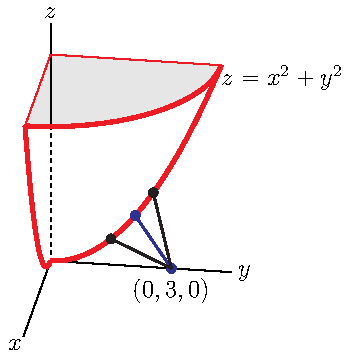
\includegraphics{distanceBB.pdf}\qquad
   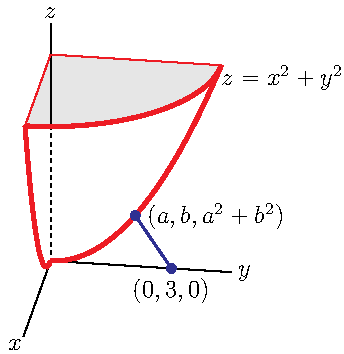
\includegraphics{distanceB.pdf}
\end{center}
\end{efig}
}
The line from $(0,3,0)$ to $\big(a,b,f(a,b)\big)$,
the point on $z=f(x,y)$ nearest $(0,3,0)$, 
is distinguished from the other lines from $(0,3,0)$ to the 
surface, by being perpendicular to the surface.
We will provide a detailed justification for this claim below. 


Let's first exploit the fact that the vector
from $(0,3,0)$ to $\big(a,b,f(a,b)\big)$ must be perpendicular to the surface
to determine $\big(a,b,f(a,b)\big)$, and consequently
the distance from $(0,3,0)$ to the surface. By Theorem \ref{thm tan plane f}.a,
with $x_0=a$ and $y_0=b$, the vector 
\begin{equation*}
-f_x(a,b)\,\hi - f_y(a,b)\,\hj +\hk
=-2a\,\hi -2b\,\hj +\hk
\tag{$*$}\end{equation*}
is normal to the surface $z=f(x,y)$ at $\big(a,b,f(a,b)\big)$.
So the vector from $(0,3,0)$ to $\big(a,b,f(a,b)\big)$, namely
\begin{equation*}
a\,\hi + (b-3)\,\hj + f(a,b)\,\hk
=a\,\hi + (b-3)\,\hj + (a^2+b^2)\,\hk
\tag{$**$}\end{equation*}
must be parallel to $(*)$. This does not force the vector $(*)$ to 
equal $(**)$, but it does force the existence of some number $t$ obeying
\begin{equation*}
a\,\hi + (b-3)\,\hj + (a^2+b^2)\,\hk
=t\big(-2a\,\hi -2b\,\hj +\hk\big)\ 
\text{or equivalently}\ 
\left\{\begin{aligned}
a&=-2a\,t\\
b-3 &= -2b\,t\\
a^2+b^2 &= t
\end{aligned}\right.
\end{equation*}
We now have a system of three equations in the three unknowns $a$, $b$ 
and $t$. If we can solve them, we will have found the point on the surface
that we want.
\begin{itemize}
\item 
The first equation is $a(1+2t)=0$ so that either $a=0$ or $t=-\frac{1}{2}$.
\item
The third equation forces $t\ge 0$, so $a=0$, and the last equation reduces to
$t=b^2$. 
\item
Substituting this into the middle equation gives
\begin{equation*}
b-3=-2b^3\qquad\text{or equivalently}\qquad
2b^3+b-3 = 0
\end{equation*}
\end{itemize}
In general, cubic equations are very hard to solve\footnote{The method 
for solving cubics was developed in the 15th century by 
del Ferro, Cardano and Ferrari (Cardano's student). Ferrari then went 
on to discover a formula for the roots of a quartic. Both the cubic and quartic
formulae are extremely cumbersome, and no such formula exists for 
polynomials of degree 5 and higher. This is the famous Abel-Ruffini theorem.}.
But, in this case,
we can guess one solution\footnote{See Appendix \eref{CLP101}{ap:roots} in the 
CLP-2 text. There it is shown that any integer root of a polynomial with 
integer coefficients must divide the constant term exactly. So in this case
only $\pm 1$ and $\pm 3$ could be integer roots. So it good to check to 
see if any of these are solutions before moving on to more sophisticated
techniques.}, namely $b=1$. So $(b-1)$
must be a factor of $2b^3+b-3$ and a little division then gives us
\begin{equation*}
0=2b^3+b-3
=(b-1)(2b^2 +2b  +3)
\end{equation*}
We can now find the roots of the quadratic factor by using
the high school formula
\begin{equation*}
\frac{-4\pm\sqrt{2^2-4(2)(3)}}{4}
\end{equation*}
Since $2^2-4(2)(3)<0$, the factor $2b^2 +2b  +3$ has no real roots. 
So the only real solution to the cubic equation $2b^3+b-3 = 0$
is $b=1$.

In summary, 
\begin{itemize} \itemindent 15pt
\item
$a=0$, $b=1$ and
\item
the point on $z=x^2+y^2$ nearest $(0,3,0)$ is $(0,1,1)$ and 
\item 
the distance from $(0,3,0)$ to $z=x^2+y^2$ is the distance from
$(0,3,0)$ to $(0,1,1)$, which is $\sqrt{(-2)^2+1^2}=\sqrt{5}$. 
\end{itemize}

Finally back to the claim that, because $\big(a,b,f(a,b)\big)$ 
is the point on $z=f(x,y)$ that is nearest\footnote{Note that we are assuming
that $\big(a,b,f(a,b)\big)$ is the point on the surface that is nearest
$(0,3,0)$. That there exists such a point is intuitively obvious from
a sketch of the surface. The mathematical proof that there exists such
a point is beyond the scope of this text.}  $(0,3,0)$, the vector
from $(0,3,0)$ to $\big(a,b,f(a,b)\big)$ must be perpendicular to the
surface $z=f(x,y)$ at $\big(a,b,f(a,b)\big)$.% 
\intremark{
We'll give two justifications. The first is geometric and the second
uses Calculus. Here is the geometric argument.
Look at the following figure. It shows a side view
of the surface $z=f(x,y)$ as well as the tangent plane to $z=f(x,y)$
at $\big(a,b,f(a,b)\big)$.

\begin{efig}
\begin{center}
   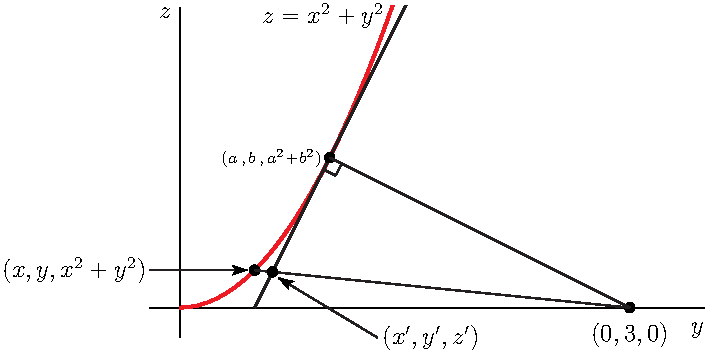
\includegraphics{distanceSide.pdf}
\end{center}
\end{efig}

Consider a general point $\big(x,y,f(x,y)\big)$ on the surface and 
denote by $(x',y',z')$ the point of intersection of the tangent plane
with the line segment from $(0,3,0)$ to $\big(x,y,f(x,y)\big)$. 
\begin{itemize}
\item 
If $x=a$ and $y=b$, then $(x',y',z')=\big(x,y,f(x,y)\big)=\big(a,b,f(a,b)\big)$
and, in particular, the distance from $(0,3,0)$ to $(x',y',z')$
is the same as the distance from $(0,3,0)$ to $\big(a,b,f(a,b)\big)$.
\item
As the point $\big(x,y,f(x,y)\big)$ moves away from $\big(a,b,f(a,b)\big)$,
the distance from $(0,3,0)$ to $\big(x',y',z'\big)$ (which is smaller than
the distance from $(0,3,0)$ to $\big(x,y,f(x,y)\big)$)
increases by Pythagoras --- the line segment from 
$(0,3,0)$ to $\big(x',y',z'\big)$ is the hypotenuse of a triangle, one of 
whose other sides is the line segment $(0,3,0)$ to $\big(a,b,f(a,b)\big)$.
\end{itemize}

Here is a Calculus justification to the claim that, because 
$\big(a,b,f(a,b)\big)$ is the point on $z=f(x,y)$ that is nearest 
$(0,3,0)$, the vector from $(0,3,0)$ to $\big(a,b,f(a,b)\big)$ 
must be perpendicular to the surface $z=f(x,y)$ at $\big(a,b,f(a,b)\big)$. 
}%
Note that the square of the distance from $(0,3,0)$ to a general point
$\big(x,y,f(x,y)\big)$ on $z=f(x,y)$ is
\begin{equation*}
D(x,y) = x^2 + (y-3)^2 +f(x,y)^2
\end{equation*}
If $x=a$, $y=b$ minimizes $D(x,y)$ then, in particular, 
\begin{itemize}
\item
  restricting our attention to the slice $y=b$ of the surface,
  $x=a$ minimizes $g(x) = D(x,b) =x^2 + (b-3)^2 +f(x,b)^2$ so that
  \begin{align*}
    0 &= g'(a) =\pdiff{}{x}\Big[x^2 + (b-3)^2 +f(x,b)^2\Big]\bigg|_{x=a}
        % \Big[2x +2 f(x,b)\ f_x(x,b)\Big]_{x=a}
       =2a +2 f(a,b)\ f_x(a,b) \\
      &=2 \llt a\,,\,b-3\,,\, f(a,b)\rgt\cdot\llt 1\,,\,0\,,\, f_x(a,b)\rgt
  \end{align*}
  and
\item
  restricting our attention to the slice $x=a$ of the surface,
  $y=b$ minimizes $h(y) = D(a,y) =a^2 + (y-3)^2 +f(a,y)^2$ so that
  \begin{align*}
    0 &= h'(b) =\pdiff{}{y}\Big[a^2 + (y-3)^2 +f(a,y)^2\Big]\bigg|_{y=b}
       %=\Big[2 (y-3) +2 f(a,y)\ f_y(a,y)\Big]_{y=b}
       =2 (b-3) +2 f(a,b)\ f_y(a,b) \\
      &=2 \llt a\,,\,b-3\,,\, f(a,b)\rgt\cdot\llt 0\,,\,1\,,\, f_y(a,b)\rgt
  \end{align*}

\end{itemize}
We have expressed the final right hand sides of both of the above bullets
as the dot product of the vector $\llt a\,,\,b-3\,,\, f(a,b)\rgt$
with something because
\begin{itemize}\itemsep1pt \parskip0pt \parsep0pt
\item[$\circ$] 
$\llt a\,,\,b-3\,,\, f(a,b)\rgt$ is the vector from $(0,3,0)$
to the point $(a\,,\,b\,,\, f(a,b)\big)$ on the surface and
\item[$\circ$] the vanishing of the dot product of two vectors
implies that the two vectors are perpendicular.
\end{itemize}
Thus, that
\begin{equation*}
\llt a\,,\,b-3\,,\, f(a,b)\rgt\cdot\llt 1\,,\,0\,,\, f_x(a,b)\rgt
=\llt a\,,\,b-3\,,\, f(a,b)\rgt\cdot\llt 0\,,\,1\,,\, f_y(a,b)\rgt
=0
\end{equation*}
 tells us that the vector $\llt a\,,\,b-3\,,\, f(a,b)\rgt$
from $(0,3,0)$ to $\big(a,b,f(a,b)\big)$ is perpendicular to both 
$\llt 1\,,\,0\,,\, f_x(a,b)\rgt$ and $\llt 0\,,\,1\,,\, f_y(a,b)\rgt$
and hence is parallel to their cross product
$\llt 1\,,\, 0\,,\, f_x(a,b)\rgt\times\llt 0\,,\, 1\,,\, f_y(a,b)\rgt$,
which we already know is a normal vector to the surface $z=f(x,y)$ at 
 $\big(a,b,f(a,b)\big)$. 

This shows that the point on the surface that minimises the distance 
to $(0,3,0)$ is joined to $(0,3,0)$ by a line that is parallel to the 
normal vector --- just as we require. 

\end{eg}

%%%%
\subsection{Surfaces of the Form $G(x,y,z)=0$.}
%%%%
We now use  a little trickery to construct a vector perpendicular to 
the surface $G(x,y,z)=0$ at the point $\big(x_0\,,\,y_0\,,\,z_0\big)$.
Imagine that you are walking on the surface and that at time $0$
you are at the point $\big(x_0\,,\,y_0\,,\,z_0\big)$. Let $\vr(t)
=\big(x(t)\,,\,y(t)\,,\,z(t)\big)$ denote your position at time $t$.
\vadjust{
\begin{efig}
\begin{center}
   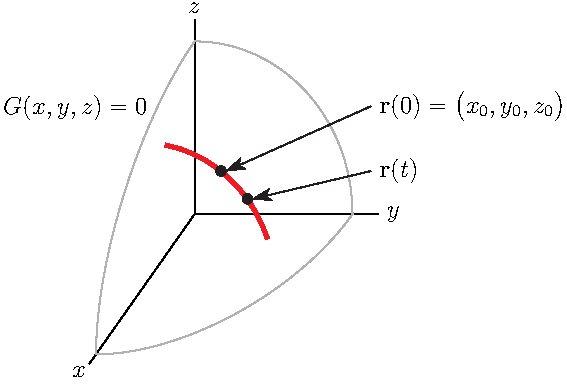
\includegraphics{tanPlaneG.pdf}
\end{center}
\end{efig}
}
Because you are walking along the surface, we know that $\vr(t)$ always 
lies on the surface and so
\begin{equation*}
G\big( x(t)\,,\,y(t)\,,\,z(t)\big)=0
\end{equation*}
for all $t$. Differentiating this equation with respect to $t$ gives,
by the chain rule,
\begin{equation*}
\pdiff{G}{x}\big( x(t)\,,\,y(t)\,,\,z(t)\big)\ x'(t)
+\pdiff{G}{y}\big( x(t)\,,\,y(t)\,,\,z(t)\big)\ y'(t)
+\pdiff{G}{z}\big( x(t)\,,\,y(t)\,,\,z(t)\big)\ z'(t) = 0
\end{equation*}
Then setting $t=0$ gives 
\begin{equation*}
\pdiff{G}{x}\big( x_0\,,\,y_0\,,\,z_0\big)\ x'(0)
+\pdiff{G}{y}\big( x_0\,,\,y_0\,,\,z_0\big)\ y'(0)
+\pdiff{G}{z}\big( x_0\,,\,y_0\,,\,z_0\big)\ z'(0) = 0
\end{equation*}
Expressing this as a dot product allows us to turn this into a 
statement about vectors.
\begin{equation*}
\llt \pdiff{G}{x}\big( x_0\,,\,y_0\,,\,z_0\big)\,,\,
     \pdiff{G}{y}\big( x_0\,,\,y_0\,,\,z_0\big)\,,\,
     \pdiff{G}{z}\big( x_0\,,\,y_0\,,\,z_0\big)\rgt \cdot \vr'(0) = 0
\tag{$*$}\end{equation*}
The first vector in this dot product is sufficiently important that it is 
given its own name.
\begin{defn}[Gradient]\label{def gradient}
The gradient\footnote{The gradient will also play a big role in 
Section \ref{sec directional derivatives}.} of the function $G(x,y,z)$ at the point 
$\big( x_0\,,\,y_0\,,\,z_0\big)$ is
\begin{equation*}
\llt \pdiff{G}{x}\big( x_0\,,\,y_0\,,\,z_0\big)\,,\,
     \pdiff{G}{y}\big( x_0\,,\,y_0\,,\,z_0\big)\,,\,
     \pdiff{G}{z}\big( x_0\,,\,y_0\,,\,z_0\big)\rgt
\end{equation*}
It is denoted $\vnabla G(x_0,y_0,z_0)$.
\end{defn}\noindent
So $(*)$ tells us that the gradient
$\vnabla G(x_0,y_0,z_0)$, is perpendicular to the vector $\vr'(0)$.

Now if $t$ is very close to zero, the vector $\vr(t)-\vr(0)$, from
$\vr(0)$ to $\vr(t)$, is almost tangent to the path that we are walking on.
The limit 
\begin{equation*}
\vr'(0)=\lim_{t\rightarrow 0}\frac{\vr(t)-\vr(0)}{t}
\end{equation*}
is thus exactly tangent to our path, and consequently to the surface
$G(x,y,z)=0$ at $(x_0,y_0,z_0)$. This is true for all paths on the surface that
pass through $(x_0,y_0,z_0)$ at time $t=0$, which tells us that
$\vnabla G(x_0,y_0,z_0)$ is perpendicular to the surface at $(x_0,y_0,z_0)$. 
We have just found a normal vector!

The above argument goes through unchanged for surfaces of 
the form\footnote{Alternatively, one could rewrite $G=K$ as $G-K=0$
and replace $G$ by $G-K$ in the above argument.}
$G(x,y,z)=K$, for any constant $K$. So we have

\begin{theorem}[Tangent Plane and Normal Line]\label{thm tan plane G}
Let $K$ be a constant and $(x_0,y_0,z_0)$ be a point on the surface 
$G(x,y,z)=K$. Assume that the gradient 
\begin{equation*}
\vnabla G(x_0,y_0,z_0)
 = \llt \pdiff{G}{x}\big( x_0\,,\,y_0\,,\,z_0\big)\,,\,
     \pdiff{G}{y}\big( x_0\,,\,y_0\,,\,z_0\big)\,,\,
     \pdiff{G}{z}\big( x_0\,,\,y_0\,,\,z_0\big)\rgt
\end{equation*}
of $G$ at $(x_0,y_0,z_0)$ is nonzero.
\begin{enumerate}[(a)]
\item 
The vector $\vnabla G(x_0,y_0,z_0)$
is normal to the surface $G(x,y,z)=K$ at $(x_0,y_0,z_0)$.

\item
The equation of the tangent plane to the surface $G(x,y,z)=K$ 
at $(x_0,y_0,z_0)$ is
\begin{equation*}
\vnabla G(x_0,y_0,z_0)\cdot\llt x-x_0\,,\,y-y_0\,,\,z-z_0\rgt =0
\end{equation*}

\item
The parametric equation of the normal line to the surface $G(x,y,z)=K$ 
at $(x_0,y_0,z_0)$ is
\begin{equation*}
\llt x,y,z \rgt =  \llt x_0,y_0,z_0 \rgt
                 +t\,\vnabla G(x_0,y_0,z_0)
\end{equation*}
\end{enumerate}
\end{theorem}


\begin{remark}\label{rem tan plane}
Theorem \ref{thm tan plane f} about the tangent planes and normal lines
to the surface $z=f(x,y)$ is actually a very simple consequence of
Theorem \ref{thm tan plane G} about the tangent planes and normal lines
to the surface $G(x,y,z)=0$. This is just because we can always 
rewrite the equation $z=f(x,y)$ as $z-f(x,y)=0$ and apply
Theorem \ref{thm tan plane G} with $G(x,y,z)=z-f(x,y)$. Since
\begin{equation*}
\vnabla G(x_0,y_0,z_0) = -f_x(x_0,y_0)\,\hi -f_y(x_0,y_0)\,\hj +\hk
\end{equation*}
Theorem \ref{thm tan plane G} then gives\footnote{Indeed we could write 
Theorem \ref{thm tan plane f} as a corollary of Theorem \ref{thm tan plane G}.
But in a textbook one tries to start with the concrete and move to the more
general.} 
Theorem \ref{thm tan plane f}.
\end{remark}

Here are a couple of routine examples.
\begin{eg}\label{eg tan plane C}
\noindent\textit{Problem}:
Find the tangent plane and the normal line to the surface
\begin{equation*}
z= x^2+5xy-2y^2
\end{equation*}
at the point $(1,2,3)$.

\medskip
\noindent\textit{Solution}. 
As a preliminary check, note that
\begin{equation*}
1^2+5\times 1\times 2-2(2)^2=3
\end{equation*} 
which verifies that the point $(1,2,3)$ is indeed on the surface.
This is a good reality check and also increases our confidence that the
question is asking what we think that it is asking.
Rewrite the equation of the surface as $G(x,y,z)=x^2+5xy-2y^2-z=0$.
Then the gradient
\begin{align*}
\vnabla G(x,y,z) = (2x+5y)\,\hi +(5x-4y)\,\hj-\hk
\end{align*}
so that, by Theorem \ref{thm tan plane G},
\begin{equation*}
\vn = \vnabla G(1,2,3) = 12\,\hi -3\,\hj-\hk
\end{equation*}
is a normal vector to the surface at $(1,2,3)$.
Equipped\footnote{The spelling ``equipt'' is a bit archaic. There must 
be a joke here about quips.} with the normal, it is easy to work out an equation for
the tangent plane.
\begin{equation*}
\vn\cdot\llt x-1\,,\,y-2\,,\,z-3 \rgt
=\llt 12\,,\,-3\,,\, -1\rgt\cdot\llt x-1\,,\,y-2\,,\,z-3 \rgt
=0\quad\text{or}\quad
12x -3y -z = 3
\end{equation*}
We can quickly check that the point $(1,2,3)$ does indeed lie on the plane:
\begin{equation*}
12\times 1 -3\times 2 -3 = 3
\end{equation*}
The normal line is
\begin{equation*}
\llt x-1\,,\,y-2\,,\,z-3 \rgt
=t\,\vn = t\llt 12\,,\,-3\,,\, -1\rgt
\quad\text{or}\quad
\frac{x-1}{12} = \frac{y-2}{-3} = \frac{z-3}{-1}\quad 
  \textcolor{gray}{\Big(=t\Big)}
\end{equation*} 

\end{eg}

Another warm-up example. This time the surface is a hyperboloid of one sheet.

\begin{eg}\label{eg tan plane D}
\noindent\textit{Problem}:
Find the tangent plane and the normal line to the surface
\begin{equation*}
x^2+y^2-z^2 = 4
\end{equation*}
at the point $(2,-3,3)$.

\medskip
\noindent\textit{Solution}. 
As a preliminary check, note that the point $(2,-3,3)$ is indeed on the surface:
\begin{equation*}
2^2+(-3)^2-(3)^2=4
\end{equation*} 
The equation of the surface is $G(x,y,z)=x^2+y^2-z^2=4$.
Then the gradient of $G$ is
\begin{align*}
\vnabla G(x,y,z) = 2x\,\hi +2y\,\hj-2z\,\hk
\end{align*}
so that, at $(2,-3,3)$,
\begin{equation*}
\vnabla G(2,-3,3) = 4\,\hi -6\,\hj-6\,\hk
\end{equation*}
and so, by Theorem \ref{thm tan plane G},
\begin{equation*}
\vn = \frac{1}{2}\big(4\,\hi -6\,\hj-6\,\hk\big)=2\,\hi-3\,\hj-3\,\hk
\end{equation*}
is a normal vector to the surface at $(2,-3,3)$. The tangent plane is
\begin{equation*}
\vn\cdot\llt x-2\,,\,y+3\,,\,z-3 \rgt
=\llt 2\,,\,-3\,,\, -3\rgt\cdot\llt x-2\,,\,y+3\,,\,z-3 \rgt
=0\quad\text{or}\quad
2x -3y -3z = 4
\end{equation*}
Again, as a check, we can verify that our point $(2,-3,3)$ is indeed on 
the plane:
\begin{equation*}
2\times 2 - 3\times(-3) -3\times 3 = 4
\end{equation*}
 The normal line is
\begin{equation*}
\llt x-2\,,\,y+3\,,\,z-3 \rgt
=t\,\vn = t\llt 2\,,\,-3\,,\, -3\rgt
\quad\text{or}\quad
\frac{x-2}{2} = \frac{y+3}{-3} = \frac{z-3}{-3}\quad 
  \textcolor{gray}{\Big(=t\Big)}
\end{equation*} 

\end{eg}

\begin{warning}\label{warn tan plane}
\emph{The vector $\vnabla G(x,y,z)$ is not a normal vector to the surface
$G(x,y,z)\!=\!K$ at $(x_0,y_0,z_0)$. The vector  $\vnabla G(x_0,y_0,z_0)$ is
a normal vector to $G(x,y,z)\!=\!K$ at $(x_0,y_0,z_0)$
(provided $G(x_0,y_0,z_0)=K$).}

\medskip

As an example of the consequences of failing to evaluate 
$\vnabla G(x,y,z)$ at the point $(x_0,y_0,z_0)$, consider the problem 
\begin{equation*}
\text{Find the tangent plane to the surface 
$x^2+y^2+z^2=1$ at the point $(0,0,1)$.}
\end{equation*}
 In this case,
the surface is $G(x,y,z)=x^2+y^2+z^2=1$. The gradient of $G$ is
$\vnabla G(x,y,z) = 2x\,\hi +2y\,\hj +2z\,\hk$. To correctly apply part (b) 
of Theorem \ref{thm tan plane G}, we evaluate
$\vnabla G(0,0,1) = 2\,\hk$ and find that the tangent plane at $(0,0,1)$ is
\begin{align*}
\vnabla G(0,0,1)\cdot\llt x-0\,,\,y-0\,,\,z-1\rgt =0
\qquad\text{or}\qquad 2(z-1)=0
\qquad\text{or}\qquad z=1
\end{align*}
This is of course correct --- the tangent plane to the unit sphere at the north
pole is indeed horizontal.

\medskip
But if we were to incorrectly apply part (b) of Theorem \ref{thm tan plane G} 
by failing to evaluate $\vnabla G(x,y,z)$ at $(0,0,1)$, we would find that 
the ``tangent plane'' is
\begin{align*}
&\vnabla G(x,y,z)\cdot\llt x-0\,,\,y-0\,,\,z-1\rgt =0 \\
\qquad\text{or}\qquad &2x(x-0) +2y(y-0) + 2z(z-1)=0 \\
\qquad\text{or}\qquad & x^2+y^2+z^2 -z = 0
\end{align*}
This is horribly wrong. It is not even a plane, as any plane has
an equation of the form $ax+by+cz=d$, with $a$, $b$, $c$ and $d$ constants.

\end{warning}

Now we'll move on to some more involved examples.


\begin{eg}\label{eg tan plane E}
Suppose that we wish to find the highest and lowest points on the 
surface $G(x,y,z) = x^2-2x +y^2-4y + z^2-6z = 2$. That is, we wish
to find the points on the surface with the maximum value of $z$
and with the minimum\footnote{Recall that ``minimum'' means the most
negative, not the closest to zero.} value of $z$.

Completing three squares,
\begin{equation*}
G(x,y,z) = x^2-2x +y^2-4y + z^2-6z
         =(x-1)^2 +(y-2)^2 +(z-3)^2 - 14.
\end{equation*}
So the surface $G(x,y,z)=2$ is a sphere, whose highest point is
the north pole and whose lowest point is the south pole. But let's
pretend that $G(x,y,z)=2$ is some complicated surface that we can't 
easily picture. 

We'll find its highest and lowest points by exploiting the
fact that the tangent plane to $G=2$ is horizontal at the highest and lowest
points. Equivalently, the normal vector to $G=2$ is vertical at the highest 
and lowest points. To see that this is the case, look at the figure below. 
If the tangent plane at $(x_0,y_0,z_0)$ is not horizontal, then the 
tangent plane contains points near $(x_0,y_0,z_0)$ with $z$ bigger 
than $z_0$ and points near $(x_0,y_0,z_0)$ with $z$ smaller than $z_0$. 
Near $(x_0,y_0,z_0)$, the tangent plane is a good approximation to the
surface. So the surface also contains\footnote{While this is intuitively
obvious, proving it is beyond the scope of this text.} such points.
\begin{efig}
\begin{center}
   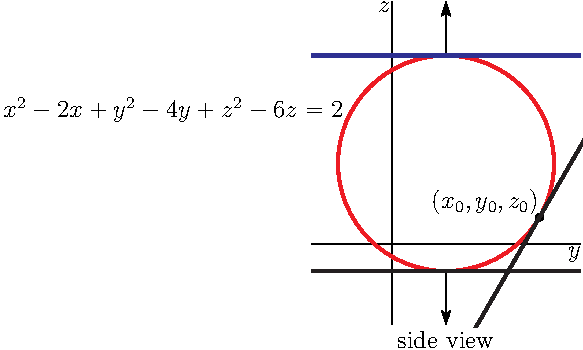
\includegraphics{highLowB.pdf}
\end{center}
\end{efig}
The gradient is
\begin{equation*}
\vnabla G(x,y,z) = (2x-2)\,\hi + (2y-4)\,\hj + (2z-6)\,\hk
\end{equation*}
It is vertical when the $\hi$ and $\hj$ components are both zero.
This happens when $2x-2=0$ and $2y-4=0$, i.e. when $x=1$ and $y=2$.
So the normal vector to the surface $G=2$ at the point $(x,y,z)$
is vertical when $x=1$, $y=2$ and (don't forget that $(x,y,z)$ has to be
on $G=2$)
\begin{align*}
&G(1,2,z) = 1^2-2\times 1 +2^2-4\times 2 + z^2-6z = 2 \\
\iff & z^2-6z-7=0 \\
\iff & (z-7)(z+1)=0 \\
\iff & z=7,\ -1
\end{align*}
The highest point is $(1,2,7)$ and the lowest point is $(1,2,-1)$,
as expected.
\end{eg}
We could have short-cut the last example by using that the surface was 
a sphere. Here is an example in the same spirit for which we don't have 
an easy short-cut.

\begin{eg}\label{eg tan plane F}
In the last example, we found the points on a specified surface 
having the largest and smallest values of $z$. We'll now ramp up the
level of difficulty a bit and find the points on the surface
$x^2+ 2y^2 +3z^2 = 72$ that have the largest and smallest values of 
$x+y+3z$.

To develop a strategy for tackling this problem, consider the
following sketch.
\vadjust{
\begin{efig}
\begin{center}
   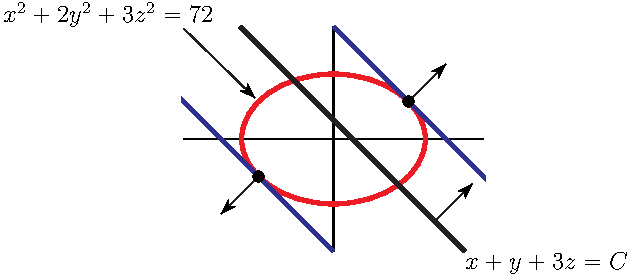
\includegraphics{bigSmall.pdf}
\end{center}
\end{efig}
}
The red ellipse in the sketch is intended to represent (schematically)
our surface 
\begin{equation*}
x^2+ 2y^2 +3z^2 = 72
\end{equation*} 
which is an ellipsoid. The middle 
diagonal (black) line is intended to represent (schematically) 
the plane $x+y+3z=C$ for some more or less randomly chosen value of 
the constant C. 
At each point on that plane, the function, $x+y+3z$, (that we are trying
to maximize and minimize) takes the value $C$. 
In particular, for the $C$ chosen in the figure, $x+y+3z=C$ does intersect
our surface, indicating that $x+y+3z$ does indeed take the value $C$
somewhere on our surface. 

To maximize $x+y+3z$, imagine slowly increasing the value of $C$.
As we do so, the plane $x+y+3z=C$ moves to the right. We want to stop
increasing $C$ at the biggest value of $C$ for which the plane $x+y+3z=C$
intersects our surface $x^2+ 2y^2 +3z^2 = 72$. For that value of $C$
the plane $x+y+3z=C$, which is represented by the right hand blue line 
in the sketch, is tangent to our surface. 

Similarly, to minimize $x+y+3z$, imagine slowly decreasing the value of $C$.
As we do so, the plane $x+y+3z=C$ moves to the left. We want to stop
decreasing $C$ at the smallest value of $C$ for which the plane $x+y+3z=C$
intersects our surface $x^2+ 2y^2 +3z^2 = 72$. For that value of $C$
the plane $x+y+3z=C$, which is represented by the left hand blue line 
in the sketch, is again tangent to our surface. The previous
Example \ref{eg tan plane E} was similar, except that the plane was
$z=C$.

We are now ready to compute. We need to find the points $(a,b,c)$
(in the sketch, they are the black dot points of tangency) for which
\begin{itemize}
\item $(a,b,c)$ is on the surface and
\item the normal vector to the surface $x^2+ 2y^2 +3z^2 = 72$
         at $(a,b,c)$ is parallel to $\llt 1,1,3\rgt$, which is 
         a normal vector to the plane $x+y+3z=C$
\end{itemize}
Since the gradient of $x^2+ 2y^2 +3z^2$ is 
$\llt 2x\,,\,4y\,,\,6z\rgt=2\llt x\,,\,2y\,,\,3z\rgt$,
these two conditions are, in equations,
\begin{align*}
a^2+ 2b^2 +3c^2 &= 72 \\
\llt a\,,\,2b\,,\,3c\rgt &=t \llt 1,1,3\rgt\qquad
\text{for some number $t$}
\end{align*}
The second equation says that $a=t$, $b=\frac{t}{2}$ and $c=t$.
Substituting this into the first equation gives
\begin{align*}
t^2+ \frac{1}{2}t^2 +3t^2 &= 72
\iff \frac{9}{2}t^2=72
\iff t^2 = 16
\iff t=\pm 4
\end{align*}
So 
\begin{itemize}
\item 
the point on the surface  $x^2+ 2y^2 +3z^2 = 72$ at which 
$x+y+3z$ takes its maximum value is $(a,b,c) = \big(t,\frac{t}{2},t\big)\Big|_{t=4}=(4,2,4)$ and
\item
$x+y+3z$ takes the value $4+2+3\times 4 =18$ there.
\item
The point on the surface  $x^2+ 2y^2 +3z^2 = 72$ at which 
$x+y+3z$ takes its minimum value is $(a,b,c) 
=\big(t,\frac{t}{2},t\big)\Big|_{t=-4}= (-4,-2,-4)$ and
\item
$x+y+3z$ takes the value $-4-2+3\times (-4) =-18$ there. 
\end{itemize} 
\end{eg}

\begin{eg}\label{eg tan plane G}
\noindent\textit{Problem}:
Find the distance from the point $(1,1,1)$ to the plane
$x+2y+3z=20$.

\medskip
\noindent\textit{Solution 1}. 
First note that the point $(1,1,1)$ is not itself on the plane 
$x+2y+3z=20$ because
\begin{equation*}
1+2\times 1 +3\times 1 =6\ne 20
\end{equation*}
Denote by $(a,b,c)$ the point on the plane $x+2y+3z=20$ that
is nearest $(1,1,1)$. Then the vector from $(1,1,1)$ to $(a,b,c)$,
namely $\llt a-1\,,\,b-1\,,\,c-1\rgt$, must be perpendicular\footnote{We
saw why this vector must be perpendicular to the plane in 
Example \ref{eg tan plane B}.} to the plane.
As the gradient of $x+2y+3z$, namely $\llt 1\,,\,2\,,\,3\rgt$,
is a normal vector to the plane, $\llt a-1\,,\,b-1\,,\,c-1\rgt$
must be parallel to $\llt 1\,,\,2\,,\,3\rgt$. So there must be some 
number $t$ so that
\begin{align*}
\llt a-1\,,\,b-1\,,\,c-1\rgt = t \llt 1\,,\,2\,,\,3\rgt\qquad\text{or}\qquad
a = t+1,\ b=2t+1,\ c=3t+1
\end{align*}
As $(a,b,c)$ must be on the plane, we know that $a+2b+3c=20$ and so
\begin{align*}
(t+1) +2(2t+1) +3(3t+1)=20
\implies 14t = 14
\implies t=1
\end{align*}
The distance from $(1,1,1)$ to the plane $x+2y+3z=20$
is the length of the vector 
  $\llt a-1\,,\,b-1\,,\,c-1\rgt = t \llt 1\,,\,2\,,\,3\rgt
  = \llt 1\,,\,2\,,\,3\rgt$
which is $\sqrt{14}$.

\begin{efig}
\begin{center}
   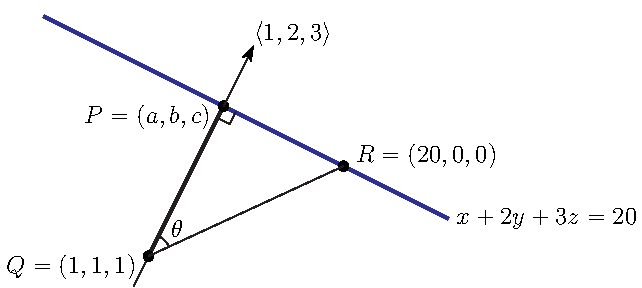
\includegraphics{distanceSideC.pdf}
\end{center}
\end{efig}



\medskip
\noindent\textit{Solution 2}. 
Denote by $P=(a,b,c)$ the point on the plane $x+2y+3z=20$ that
is nearest the point $Q=(1,1,1)$. Pick any other point on the plane
and call it $R$. For example
$(x,y,z) = (20,0,0)$ obeys $x+2y+3z=20$  and so $R=(20,0,0)$ is a point 
on the plane. 

The triangle $PQR$ is right angled. Denote by $\theta$
the angle between the hypotenuse $QR$ and the side $QP$.
The distance from $Q=(1,1,1)$ to the plane is the length of the 
line segment $QP$, which is
\begin{align*}
\text{distance} &= |QP| = |QR|\cos\theta
\end{align*} 
Now, the dot product between the vector from $Q$ to $R$, which is 
$\llt 19,-1,-1\rgt$, with the vector $\llt 1,2,3\rgt$, which is 
normal to the plane and hence parallel to the side $QP$ is
\begin{align*}
 \llt 19,-1,-1\rgt\cdot \llt 1,2,3\rgt &=14 \\
   &= |\llt 19,-1,-1\rgt|\  |\llt 1,2,3\rgt|\ \cos\theta
   = |QR|\  \sqrt{14}\ \cos\theta
\end{align*}
so that, finally,
\begin{align*}
\text{distance} = |QR|\cos\theta =\frac{14}{\sqrt{14}}=\sqrt{14}
\end{align*}

\end{eg}

\begin{eg}\label{eg tan plane H}
\noindent\textit{Problem}:
Let $F(x,y,z)=0$ and $G(x,y,z)=0$ be two surfaces. These two surfaces
intersect along a curve.
Find a tangent vector to this curve at the point $(x_0,y_0,z_0)$.

\medskip
\noindent\textit{Solution}.
Call the tangent vector $\vT$. Then $\vT$ has to be
\begin{itemize}\itemsep1pt \parskip0pt \parsep0pt
\item[$\circ$] 
tangent to the surface  $F(x,y,z)=0$ at $(x_0,y_0,z_0)$ and
\item[$\circ$] 
tangent to the surface  $G(x,y,z)=0$ at $(x_0,y_0,z_0)$.
\end{itemize}
Consequently $\vT$ has to be 
\begin{itemize}\itemsep1pt \parskip0pt \parsep0pt
\item[$\circ$] 
perpendicular to the vector $\vnabla F(x_0,y_0,z_0)$, which is
normal to  $F(x,y,z)=0$ at $(x_0,y_0,z_0)$, and at the same time has to be
\item[$\circ$] 
perpendicular to the vector $\vnabla G(x_0,y_0,z_0)$, which is
normal to  $G(x,y,z)=0$ at $(x_0,y_0,z_0)$.
\end{itemize}
Recall that an easy way to construct a vector that is perpendicular to
two other vectors is to take their cross product. So we take
\begin{align*}
\vT &= \vnabla F(x_0,y_0,z_0)\times \vnabla G(x_0,y_0,z_0)
    =\det\left[\begin{matrix}
                 \hi & \hj & \hk \\
                 F_x & F_y & F_z \\
                 G_x & G_y & G_z \end{matrix}\right] \\
& =\big(F_yG_z-F_z G_y\big)\,\hi + \big(F_zG_x-F_x G_z\big)\,\hj
    +\big(F_xG_y-F_y G_x\big)\,\hk
\end{align*}
where all partial derivatives are evaluated at $(x,y,z)=(x_0,y_0,z_0)$.

\end{eg}

Let's put Example \ref{eg tan plane H} into action.


\begin{eg}\label{eg tan plane I}
\noindent\textit{Problem}:
Consider the curve that is the intersection of the surfaces
\begin{equation*}
x^2+y^2+z^2=5\qquad\text{and}\qquad
x^2+y^2=4z
\end{equation*}
Find a tangent vector to this curve 
at the point $\big(\sqrt{3}\,,\,1\,,\,1\big)$.

\medskip
\noindent\textit{Solution}.
As a preliminary check, we verify that the point $\big(\sqrt{3}\,,\,1\,,\,1\big)$ really is on the curve. To do so,
we check that $\big(\sqrt{3}\,,\,1\,,\,1\big)$ satisfies both equations:
\begin{equation*}
\big(\sqrt{3}\big)^2+1^2+1^2=5\qquad
\big(\sqrt{3}\big)^2+1^2=4\times 1
\end{equation*}
We'll find the specified tangent vector by using the strategy of 
Example \ref{eg tan plane H}. 

Write $F(x,y,z) = x^2+y^2+z^2$
and $G(x,y,z) = x^2+y^2-4z$. Then
\begin{itemize}\itemsep1pt \parskip0pt \parsep0pt %\itemindent0.25in
\item[$\circ$] 
the vector 
\begin{equation*}
\vnabla F(\sqrt{3},1,1)
 =\llt 2x\,,\,2y\,,\,2z \rgt\Big|_{(x,y,z)=(\sqrt{3},1,1)}
 = 2\llt \sqrt{3}\,,\,1\,,\,1 \rgt
\end{equation*} 
is normal to the surface $F(x,y,z)$ at $\big(\sqrt{3}\,,\,1\,,\,1\big)$,
and
\item[$\circ$] 
the vector 
\begin{equation*}
\vnabla G(\sqrt{3},1,1)
 =\llt 2x\,,\,2y\,,\,-4 \rgt\Big|_{(x,y,z)=(\sqrt{3},1,1)}
 = 2\llt \sqrt{3}\,,\,1\,,\,-2 \rgt
\end{equation*} 
is normal to the surface $G(x,y,z)$ at $\big(\sqrt{3}\,,\,1\,,\,1\big)$.
\end{itemize}
So a tangent vector is
\begin{align*}
\llt \sqrt{3}\,,\,1\,,\,1 \rgt\times \llt \sqrt{3}\,,\,1\,,\,-2 \rgt
    &=\det\left[\begin{matrix}
                 \hi & \hj & \hk \\
            \sqrt{3} &  1  & 1 \\
            \sqrt{3} &  1  & -2 \end{matrix}\right] \\
& =\big(-2-1\big)\,\hi + \big(\sqrt{3}+2\sqrt{3}\big)\,\hj
    +\big(\sqrt{3}-\sqrt{3}\big)\,\hk \\
&= -3\,\hi + 3\sqrt{3}\,\hj
\end{align*}
There is an easy common factor of $3$ in both components. So
we can create a slightly neater tangent vector by dividing the length 
of $-3\,\hi + 3\sqrt{3}\,\hj$ by $3$, giving  $\llt -1\,,\,\sqrt{3}\,,\,0\rgt$.
\end{eg}

Tangent planes, in addition to being geometric objects, provide a 
simple but powerful tool for approximating functions of two variables
near a specified point. We saw something very similar in the CLP-1 text 
where we approximated functions of one variable by their tangent lines. 
This brings us to our next topic --- approximating functions.
 

%%%%%%%%%%%%%%%%%%%
\section{Linear Approximations and Error}\label{sec lin approx}
%%%%%%%%%%%%%%%%%%%


A frequently used, and effective, strategy for building an understanding
of the behaviour of a complicated function near a point is to
approximate it by a simple function. The following suite of such
approximations is standard fare in Calculus I courses. 
See, for example, \S\eref{CLP100}{sec:DIFFTaylor} in the CLP-1 text.
\begin{align*}
g(t_0+\De t) &\approx g(t_0) 
                   &&\text{constant approximation} \\
g(t_0+\De t) &\approx g(t_0) +g'(t_0)\,\De t  
                    &&\text{linear, or tangent line, approximation} \\
g(t_0+\De t) &\approx g(t_0) +g'(t_0)\,\De t +\tfrac{1}{2} g''(t_0)\,\De t^2
                    &&\text{quadratic approximation} 
\end{align*}
More generally, for any natural number $n$, the  approximation 
\begin{align*}
g(t_0+\De t) &\approx g(t_0) +g'(t_0)\,\De t + \tfrac{1}{2} g''(t_0)\,\De t^2
                    +\cdots+ \tfrac{1}{n!} g^{(n)}(t_0)\,\De t^n
\end{align*}
is known as the Taylor polynomial of degree $n$. 
You may have also found a formula for the error introduced in making this 
approximation. The error $E_n(\De t)$ is defined by
\begin{align*}
g(t_0+\De t)
&=
g(t_0)+g'(t_0)\De t+\tfrac{1}{2!}g''(t_0)\De t^2
+\cdots
+\tfrac{1}{n!}g^{(n)}(t_0) \De t^n +E_n(\De t)
\end{align*}
and obeys\footnote{You may have seen it written as 
$E_n(x)=\tfrac{1}{(n+1)!}g^{(n+1)}(c) (x-a)^{n+1}$}
\begin{equation*}
E_n(\De t)=
\tfrac{1}{(n+1)!}g^{(n+1)}(t_0+c\De t) \De t^{n+1}
\end{equation*}
for some (unknown) $0\le c\le 1$. 

It is a simple matter to use these one dimensional approximations 
to generate the analogous multidimensional approximations. To introduce 
the ideas, we'll generate the linear approximation to a function, 
$f(x,y)$, of two variables, near the point $(x_0,y_0)$. Define
\begin{equation*}
g(t) = f\big(x_0+t\,\De x\,,\,y_0+t\,\De y\big)
\end{equation*}
We have defined $g(t)$ so that
\begin{equation*}
g(0) = f\big(x_0\,,\,y_0\big)\qquad\text{and}\qquad
g(1) = f\big(x_0 + \De x\,,\,y_0+\De y\big)
\end{equation*}
Consequently, setting $t_0=0$ and $\De t=1$, 
%and treating $x_0$, $y_0$, $\De x$ and $\De y$ as constants,
\begin{align*}
f\big(x_0+\De x\,,\,y_0+\De y\big)
&=g(1) = g(t_0+\De t) \\
&\approx g(t_0) + g'(t_0)\,\De t \\
&= g(0) + g'(0)
\end{align*}
We can now compute $g'(0)$ using the multivariable chain rule of 
\eqref{eqn chain rule A}:
\begin{equation*}
g'(t) = \pdiff{f}{x}\big(x_0+t\,\De x\,,\,y_0+t\,\De y\big)\,\De x
       + \pdiff{f}{y}\big(x_0+t\,\De x\,,\,y_0+t\,\De y\big)\,\De y
\end{equation*}
so that, 
\begin{impeqn}\label{eqn lin approx 2d}
\begin{align*}
f\big(x_0+\De x\,,\,y_0+\De y\big)
&\approx f\big(x_0\,,\,y_0\big) 
       + \pdiff{f}{x}\big(x_0\,,\,y_0\big)\,\De x
       + \pdiff{f}{y}\big(x_0\,,\,y_0\big)\,\De y
\end{align*}
\end{impeqn}\noindent
%The right hand side should look familiar --- see part (b) of 
%Theorem \ref{thm tan plane f}.
Of course exactly the same procedure works for functions of three or 
more variables. In particular 
\begin{impeqn}\label{eqn lin approx 3d}
\begin{align*}
&f\big(x_0+\De x\,,\,y_0+\De y\,,\,z_0 + \De z\big) \\
&\hskip0.25in\approx f\big(x_0\,,\,y_0\,,\,z_0\big) 
       + \pdiff{f}{x}\big(x_0\,,\,y_0\,,\,z_0\big)\,\De x
       + \pdiff{f}{y}\big(x_0\,,\,y_0\,,\,z_0\big)\,\De y
       + \pdiff{f}{z}\big(x_0\,,\,y_0\,,\,z_0\big)\,\De z
\end{align*}
\end{impeqn}\noindent
While these linear approximations are quite simple, they tend to be 
pretty decent provided $\De x$ and $\De y$ are small. See the 
optional \S\ref{sec error} for a more precise statement.

\begin{remark}\label{rmk lin approx tan plane}
Applying \eqref{eqn lin approx 2d}, with $\De x=x-x_0$ and $\De y = y-y_0$.
gives
\begin{align*}
f\big(x\,,\,y\big)
&\approx f\big(x_0\,,\,y_0\big) 
       + \pdiff{f}{x}\big(x_0\,,\,y_0\big)\,(x-x_0)
       + \pdiff{f}{y}\big(x_0\,,\,y_0\big)\,(y-y_0)
\end{align*}
Looking at part (b) of Theorem \ref{thm tan plane f},
we see that this just says that the tangent plane to the surface 
$z=f(x,y)$ at the point $\big(x_0\,,\,y_0\,,\,f(x_0,y_0)\big)$
remains close to the surface when $(x,y)$ is close to $(x_0,y_0)$.
\end{remark}


\begin{eg}\label{eg approx AA}
Let 
\begin{equation*}
f(x,y) = \sqrt{x^2+y^2}
\end{equation*}
Then
\begin{align*}
\pdiff{f}{x}(x,y)&=\frac{1}{2}\,\frac{2x}{\sqrt{x^2+y^2}} &
    f_x(x_0,y_0)&=\frac{x_0}{\sqrt{x_0^2+y_0^2}} \\
\pdiff{f}{y}(x,y)&=\frac{1}{2}\,\frac{2y}{\sqrt{x^2+y^2}} &
    f_y(x_0,y_0)&=\frac{y_0}{\sqrt{x_0^2+y_0^2}} 
\end{align*}
so that the linear approximation to $f(x,y)$ at $(x_0,y_0)$ is
\begin{align*}
f\big(x_0+\De x\,,\,y_0+\De y\big)
&\approx f\big(x_0\,,\,y_0\big) 
       + f_x\big(x_0\,,\,y_0\big)\,\De x
       + f_y\big(x_0\,,\,y_0\big)\,\De y \\[0.05in]
&=\sqrt{x_0^2+y_0^2} 
       + \frac{x_0}{\sqrt{x_0^2+y_0^2}}\,\De x
       + \frac{y_0}{\sqrt{x_0^2+y_0^2}}\,\De y 
\end{align*}

\end{eg}

\begin{notn}\label{notn approx}
People often write $\De f$ for the change 
$f\big(x_0+\De x\,,\,y_0+\De y\big)
  - f\big(x_0\,,\,y_0\big)$ in the value of $f$. 
Then the linear approximation \eqref{eqn lin approx 2d} becomes
\begin{align*}
\De f
&\approx  \pdiff{f}{x}\big(x_0\,,\,y_0\big)\,\De x
       + \pdiff{f}{y}\big(x_0\,,\,y_0\big)\,\De y
\end{align*}
If they want to emphasize that that $\De x$, $\De y$ and $\De f$
are really small (they may even say ``infinitesimal''), they'll
write\footnote{Don't take the notation $\dee{x}$ or the terminology
``infinitesimal'' too seriously. It is just intended to signal ``very small''.} $\dee{x}$, $\dee{y}$ and $\dee{f}$ instead. In this notation
\begin{align*}
\dee{f}
&\approx  \pdiff{f}{x}\big(x_0\,,\,y_0\big)\,\dee{x}
       + \pdiff{f}{y}\big(x_0\,,\,y_0\big)\,\dee{y}
\end{align*}
\end{notn}

\begin{defn}\label{def error}
Suppose that we wish to approximate a quantity $Q$ and that the
approximation turns out to be $Q+\De Q$. Then
\begin{itemize}\itemsep1pt \parskip0pt \parsep0pt
\item 
the absolute error in the approximation is $|\De Q|$ and
\item
the relative error in the approximation is $\left|\frac{\De Q}{Q}\right|$ and
\item
the percentage error in the approximation is
$100\left|\frac{\De Q}{Q}\right|$ 
\end{itemize}
\end{defn}

In Example 3.4.5 of the CLP-1 text we found an approximate
value for the number $\sqrt{4.1}$ by using a linear approximation
to the single variable function $f(x)=\sqrt{x}$. We can make similar use
of linear approximations to multivariable functions.

\begin{eg}\label{eg approx A}
\noindent\textit{Problem}:
Find an approximate value for $\frac{(0.998)^3}{1.003}$.

\medskip
\noindent\textit{Solution}:
Set $f(x,y) = \dfrac{x^3}{y}$. We are to find (approximately) 
$f(0.998\,,\,1.003)$. We can easily find
\begin{align*}
f(1,1) &= \frac{1^3}{1}=1
\end{align*}
and since 
\begin{equation*}
\pdiff{f}{x}=\frac{3x^2}{y}\qquad \text{and}\qquad 
\pdiff{f}{y}=-\frac{x^3}{y^2}
\end{equation*}
we can also easily find
\begin{align*}
\pdiff{f}{x}(1,1) &= 3\frac{1^2}{1}=3 \\
\pdiff{f}{y}(1,1) &= 1\frac{1^3}{1^2}=-1 
\end{align*}
So, setting $\De x=-0.002$ and $\De y=0.003$, we have
\begin{align*}
\frac{0.998^3}{1.003}
&=f(0.998\,,\,1.003)
=f(1+\De x\,,\,1+\De y)
\approx f\big(1,1\big) 
       + \pdiff{f}{x}\big(1,1\big)\,\De x
       + \pdiff{f}{y}\big(1,1\big)\,\De y \\
&\approx 1 +3(-0.002)-1(0.003)
=0.991
\end{align*}
By way of comparison, the exact answer is $0.9910389$ to seven decimal places.
\end{eg}


\begin{eg}\label{eg approx B}
\noindent\textit{Problem}:
Find an approximate value for $(4.2)^{1/2} + (26.7)^{1/3} + (256.4)^{1/4}$.

\medskip
\noindent\textit{Solution}:
Set $f(x,y,z) = x^{1/2} + y^{1/3} + z^{1/4}$. We are to find (approximately) 
$f(4.2\,,\,26.7\,,\,256.4)$. We can easily find
\begin{align*}
f(4,27,256) &= (4)^{1/2} + (27)^{1/3} + (256)^{1/4} = 2+3+4 =9
\end{align*}
and since 
\begin{equation*}
\pdiff{f}{x}=\frac{1}{2x^{1/2}}\qquad
\pdiff{f}{y}=\frac{1}{3y^{2/3}}\qquad
\pdiff{f}{z}=\frac{1}{4z^{3/4}}
\end{equation*}
we can also easily find
\begin{align*}
\pdiff{f}{x}(4,27,256) &= \frac{1}{2(4)^{1/2}} =\frac{1}{2}\times\frac{1}{2} \\
\pdiff{f}{y}(4,27,256) &= \frac{1}{3(27)^{2/3}}=\frac{1}{3}\times\frac{1}{9} \\
\pdiff{f}{z}(4,27,256) &= \frac{1}{4(256)^{3/4}}=\frac{1}{4}\times\frac{1}{64}
\end{align*}
So, setting $\De x=0.2$, $\De y=-0.3$, and $\De z=0.4$, we have
\begin{align*}
&(4.2)^{1/2} + (26.7)^{1/3} + (256.4)^{1/4}
=f(4.2\,,\,26.7\,,\,256.4)
=f(4+\De x\,,\,27+\De y\,,\,256+\De z) \\
&\hskip1in\approx f\big(4,27,256\big) 
       + \pdiff{f}{x}\big(4,27,256\big)\,\De x
       + \pdiff{f}{y}\big(4,27,256\big)\,\De y 
       + \pdiff{f}{z}\big(4,27,256\big)\,\De z \\
&\hskip1in\approx 9 +\frac{0.2}{2\times2}-\frac{0.3}{3\times9}
            +\frac{0.4}{4\times64}
 = 9+\frac{1}{20}-\frac{1}{90}+\frac{1}{640}
=9.0405
\end{align*}
to four decimal places.
The exact answer is $9.03980$ to five decimal places.
%9.039799219
That's a difference of about
\begin{equation*}
100\frac{9.0405-9.0398}{9}\%
=0.008\%
\end{equation*}
Note that we could have used the single variable approximation techniques
in the CLP-1 text to separately approximate 
$(4.2)^{1/2}$, $(26.7)^{1/3}$  and $(256.4)^{1/4}$ and then added 
the results together. Indeed what we have done here is equivalent.
\end{eg}

\begin{eg}\label{eg error C}
\noindent\textit{Problem}:
A triangle has sides $a=10.1$cm and $b=19.8$cm which include an 
angle $35^\circ$. Approximate the area of the triangle.

\begin{efig}
\begin{center}
   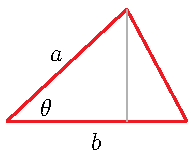
\includegraphics{triangleError.pdf}
\end{center}
\end{efig}

\medskip
\noindent\textit{Solution}:
The triangle has height $h=a\sin\theta$ and hence has area
\begin{equation*}
A(a,b,\theta) = \frac{1}{2} bh =\frac{1}{2} ab\sin\theta
\end{equation*}
The $\sin\theta$ in this formula hides a booby trap built into this problem.
In preparing the linear approximation we will need to use the derivative
of $\sin\theta$. But the standard derivative $\diff{\hfill}{\theta}\sin\theta
=\cos\theta$ only applies when $\theta$ is expressed in radians --- not in
degrees. See Warning \eref{CLP100}{warning:radians} in the CLP-1 text.

So we are obliged to convert $35^\circ$ into
\begin{equation*}
35^\circ = (30+5) \frac{\pi}{180}\ \text{radians}
         =\Big(\frac{\pi}{6} + \frac{\pi}{36}\Big)\ \text{radians}
\end{equation*}
We need to compute (approximately) 
$A(10.1\,,\,19.8\,,\,\nicefrac{\pi}{6}+\nicefrac{\pi}{36}\big)$.
We will, of course\footnote{There are other choices possible.
For example, we could write $35^\circ=45^\circ-10^\circ$. To get a good
approximation we try to make $\De\theta$ as small as possible, while 
keeping the arithmetic reasonably simple.}, choose 
\begin{align*}
a_0&=10    &  b_0&=20    & \theta_0&=\nicefrac{\pi}{6} \\
\De a&=0.1 & \De b&=-0.2 & \De\theta&=\nicefrac{\pi}{36}
\end{align*}
By way of preparation, we evaluate
\begin{align*}
A\big(a_0,b_0,\theta_0\big)
&=\frac{1}{2}a_0b_0\sin\theta_0 =\frac{1}{2}(10)(20)\frac{1}{2}=50 \\
\pdiff{A}{a}\big(a_0,b_0,\theta_0\big)
&=\frac{1}{2}b_0\sin\theta_0 =\frac{1}{2}(20)\frac{1}{2} =5 \\
\pdiff{A}{b}\big(a_0,b_0,\theta_0\big)
&=\frac{1}{2}a_0\sin\theta_0 =\frac{1}{2}(10)\frac{1}{2} =\frac{5}{2} \\
\pdiff{A}{\theta}\big(a_0,b_0,\theta_0\big)
&=\frac{1}{2}a_0b_0\cos\theta_0 =\frac{1}{2}(10)(20)\frac{\sqrt{3}}{2} 
 = 50\,\sqrt{3}
\end{align*}
So the linear approximation gives
\begin{align*}
\text{Area} & = A(10.1\,,\,19.8\,,\,\nicefrac{\pi}{6}+\nicefrac{\pi}{36}\big)
              = A(a_0+\De a\,,\,b_0+\De b\,,\,\theta_0+\De\theta\big) \\
&\approx A\big(a_0,b_0,\theta_0\big)
    + \pdiff{A}{a}\big(a_0,b_0,\theta_0\big)\De a
    + \pdiff{A}{b}\big(a_0,b_0,\theta_0\big)\De b
    + \pdiff{A}{\theta}\big(a_0,b_0,\theta_0\big)\De\theta \\
&=50 +5\times 0.1  +\frac{5}{2}\times (-0.2) +50\sqrt{3}\frac{\pi}{36} \\
&=50 +\frac{5}{10}  -\frac{5}{10} +50\sqrt{3}\frac{\pi}{36} \\
&=50\left(1+\sqrt{3}\frac{\pi}{36}\right) \\
&\approx 57.56  %57.557497351
\end{align*}
to two decimal places. The exact answer is %$57.351907871$
$57.35$ to two decimal places. Our
approximation has an error of about
\begin{equation*}
100\ \frac{57.56-57.35}{57.35}\%
=0.37\%
\end{equation*}
\end{eg}

Another practical use of these linear approximations is to quantify
how errors made in measured quantities propagate in computations
using those measured quantities. Let's explore this idea a little
by recycling the last example.

\begin{eg}[Example \ref{eg error C}, continued]\label{eg error D}
Suppose, that, as in Example \ref{eg error C}, we are attempting
to determine the area of a triangle by measuring the lengths of two of its 
sides together with the angle between them and then using the formula
\begin{equation*}
A(a,b,\theta) = \frac{1}{2} ab\sin\theta
\end{equation*}
Of course, in the real world\footnote{Of course in our ``real world'' everyone uses calculus.}, we cannot measure lengths and angles exactly. So if we need
to know the area to within 1\%,  the question becomes: ``How accurately 
do we have to measure the side lengths
and included angle if we want the area that we compute to have 
an error of no more than about 1\%?''

Let's call the exact side lengths and included angle $a_0$, $b_0$ and
$\theta_0$, respectively, and the measured side lengths and included 
angle $a_0+\De a$, $b_0+\De b$ and $\theta_0+\De\theta$.
So $\De a$, $\De b$ and $\De\theta$ represent the errors in our 
measurements. Then, by \eqref{eqn lin approx 3d}, the
error in our computed area will be approximately
\begin{align*}
\De A &\approx \pdiff{A}{a}\big(a_0,b_0,\theta_0\big)\,\De a
    + \pdiff{A}{b}\big(a_0,b_0,\theta_0\big)\,\De b
    + \pdiff{A}{\theta}\big(a_0,b_0,\theta_0\big)\,\De\theta \\
&=\frac{\De a}{2} b_0\sin\theta_0
   +\frac{\De b}{2} a_0\sin\theta_0
   +\frac{\De \theta}{2} a_0b_0\cos\theta_0
\end{align*}
and the percentage error in our computed area will be
\begin{align*}
100\frac{|\De A|}{A(a_0,b_0,\theta_0)}
&\approx \left|  100\frac{\De a}{a_0} + 100\frac{\De b}{b_0} 
                  +100\De\theta\frac{\cos\theta_0}{\sin\theta_0} \right| 
\end{align*}
By the triangle inequality, $|u+v|\le |u|+|v|$, and the fact that 
$|uv|=|u|\ |v|$,
\begin{align*}
\left|  100\frac{\De a}{a_0} + 100\frac{\De b}{b_0} 
                  +100\De\theta\frac{\cos\theta_0}{\sin\theta_0} \right| 
&\le 100\left|\frac{\De a}{a_0}\right| + 100\left|\frac{\De b}{b_0} \right|
             +100|\De\theta|\ \left|\frac{\cos\theta_0}{\sin\theta_0} \right|
\end{align*}
We want this to be less than $1$.


Of course we do not know exactly what $a_0$, $b_0$ and $\theta_0$ are.
But suppose that we are confident that $a_0\ge 10$, $b_0\ge 10$
and $\frac{\pi}{6}\le \theta_0 \le \frac{\pi}{2}$ so that 
$\cot\theta_0\le \sqrt{3}\le 2$. Then 
\begin{align*}
100\left|\frac{\De a}{a_0}\right|&\le 100\left|\frac{\De a}{10}\right|
                                 = 10\,|\De a| \\
 100\left|\frac{\De b}{b_0} \right|&\le  100\left|\frac{\De b}{10} \right|
                                = 10\,|\De b| \\
100|\De\theta|\ \left|\frac{\cos\theta_0}{\sin\theta_0} \right|
       &\le 100|\De\theta|\ 2 
       =200\,|\De\theta|
\end{align*}
and
\begin{align*}
100\frac{|\De A|}{A(a_0,b_0,\theta_0)}
\lesssim 10\,|\De a| + 10\,|\De b| +200\,|\De\theta|
\end{align*} 
So it will suffice to have
measurement errors $|\De a|$, $|\De b|$ and $|\De\theta|$ obey
\begin{equation*}
10\,|\De a| + 10\,|\De b| +200\,|\De\theta|<1
\end{equation*}
\end{eg}
\goodbreak





\begin{eg}\label{eg errors in measurement}
\noindent\textit{A Question}:

Suppose that three variables are measured with percentage
error $\veps_1,\ \veps_2$ and $\veps_3$ respectively. In other words,
if the exact value of  variable number $i$ is $x_i$ and measured value
of variable  number $i$ is $x_i+\De x_i$ then
\begin{equation*}
100\ \left|\frac{\De x_i}{x_i}\right|=\veps_i
\end{equation*}
Suppose further that a quantity $P$ is then computed by taking the 
product of the three variables. So the exact value of $P$ is
\begin{equation*}
P(x_1,x_2,x_3)=x_1x_2x_3
\end{equation*}
and the measured value is $P(x_1+\De x_1\,,\,x_2+\De x_2\,,\,x_3+\De x_3)$.
What is the percentage error in this measured value of $P$?

\medskip
\noindent\textit{The Answer}:

The percentage error in the measured value  
$P(x_1+\De x_1\,,\,x_2+\De x_2\,,\,x_3+\De x_3)$ is
\begin{equation*}
100\ \left|\frac{P(x_1+\De x_1\,,\,x_2+\De x_2\,,\,x_3+\De x_3)-P(x_1,x_2,x_3)}
               {P(x_1,x_2,x_3)}\right|
\end{equation*}
We can get a much simpler approximate expression for this percentage error,
which is good enough for virtually all applications, by applying
\begin{align*}
P(x_1+\De &x_1\,,\,x_2+\De x_2\,,\,x_3+\De x_3) \\
&\approx P(x_1,x_2,x_3) +P_{x_1}(x_1,x_2,x_3)\,\De x_1
+P_{x_2}(x_1,x_2,x_3)\,\De x_2+P_{x_3}(x_1,x_2,x_3)\,\De x_3
\end{align*}
The three partial derivatives are
\begin{alignat*}{3}
P_{x_1}(x_1,x_2,x_3)&=\pdiff{}{x_1}\big[x_1x_2x_3\big]
&=x_2x_3\cr
P_{x_2}(x_1,x_2,x_3)&=\pdiff{}{x_2}\big[x_1x_2x_3\big]
&=x_1x_3\cr
P_{x_3}(x_1,x_2,x_3)&=\pdiff{}{x_3}\big[x_1x_2x_3\big]
&=x_1x_2
\end{alignat*}
So 
\begin{equation*}
P(x_1+\De x_1\,,\,x_2+\De x_2\,,\,x_3+\De x_3)
\approx P(x_1,x_2,x_3) +x_2x_3\,\De x_1+x_1x_3\,\De x_2+x_1x_2\,\De x_3
\end{equation*}
and the (approximate) percentage error in $P$ is
\begin{align*}
&100\ \left|
  \frac{P(x_1+\De x_1,x_2+\De x_2,x_3+\De x_3)-P(x_1,x_2,x_3)}{P(x_1,x_2,x_3)}
   \right|
\\
&\hskip2in\approx 
       100\ \left|
         \frac{x_2x_3\De x_1+x_1x_3\De x_2+x_1x_2\De x_3}{P(x_1,x_2,x_3)}
       \right| \\
&\hskip2in=100\ 
  \left|\frac{x_2x_3\De x_1+x_1x_3\De x_2+x_1x_2\De x_3}{x_1x_2x_3}\right| \\
&\hskip2in=\left|100\frac{\De x_1}{x_1}+100\frac{\De x_2}{x_2}
         +100\frac{\De x_3}{x_3}\right| \\
&\hskip2in\le \veps_1+\veps_2+\veps_3
\end{align*}
More generally, if we take a product of $n$, rather than three,  variables
the percentage error in the product becomes at most (approximately)
$\ 
\smsum\limits_{i=1}^n\veps_i.
\ $
This is the basis of the experimentalist's rule of thumb that when you
take products, percentage errors add.

Still more generally, if we take a ``product'' 
  $\prod_{i=1}^n x_i^{m_i}$, the percentage error in the ``product'' becomes at most (approximately)
$\ 
\smsum\limits_{i=1}^n|m_i|\veps_i.
\ $


\end{eg}


\subsection{Quadratic Approximation and Error Bounds}\label{sec error}
Recall that, in the CLP-1 text, we started with the constant approximation,
then improved it to the linear approximation by adding in degree one terms,
then improved that to the quadratic approximation by adding in degree two
terms, and so on. We can do the same thing here.
Once again, set 
\begin{equation*}
g(t) = f\big(x_0+t\,\De x\,,\,y_0+t\,\De y\big)
\end{equation*}
and recall that
\begin{equation*}
g(0) = f\big(x_0\,,\,y_0\big)\qquad\text{and}\qquad
g(1) = f\big(x_0 + \De x\,,\,y_0+\De y\big)
\end{equation*}
We'll now see what the quadratic approximation
\begin{equation*}
g(t_0+\De t) \approx g(t_0) +g'(t_0)\,\De t +\tfrac{1}{2} g''(t_0)\,\De t^2
\end{equation*}
and the corresponding exact formula (see (\eref{CLP100}{eq:taylorErrorQ})
in the CLP-1 text)
\begin{equation*}
g(t_0+\De t) = g(t_0) +g'(t_0)\,\De t +\tfrac{1}{2} g''(t_0+c\De t)\,\De t^2
                    \qquad\text{for some $0\le c\le 1$} 
\end{equation*}
tells us about $f$. We have already found, using the chain rule, that
\begin{equation*}
g'(t) = \pdiff{f}{x}\big(x_0+t\,\De x\,,\,y_0+t\,\De y\big)\,\De x
       + \pdiff{f}{y}\big(x_0+t\,\De x\,,\,y_0+t\,\De y\big)\,\De y
\end{equation*}
We now need to evaluate $g''(t)$. Temporarily write $f_1=\pdiff{f}{x}$
and $f_2=\pdiff{f}{y}$ so that
\begin{equation*}
g'(t) = f_1\big(x_0+t\,\De x\,,\,y_0+t\,\De y\big)\,\De x
       + f_2\big(x_0+t\,\De x\,,\,y_0+t\,\De y\big)\,\De y
\end{equation*}
Then we have, again using the chain rule,
\begin{align*}
&\diff{}{t}\left[f_1\big(x_0+t\,\De x\,,\,y_0+t\,\De y\big)\right]
=\frac{\partial f_1}{\partial x}\big(x_0+t\,\De x\,,\,y_0+t\,\De y\big)
                                                                  \,\De x
 +\frac{\partial f_1}{\partial y}
              \big(x_0+t\,\De x\,,\,y_0+t\,\De y\big) \,\De y \\
&\hskip1in
=\frac{\partial^2 f}{\partial x^2}\big(x_0+t\,\De x\,,\,y_0+t\,\De y\big)
                                                                  \,\De x
 +\frac{\partial^2\ f}{\partial y\partial x}
              \big(x_0+t\,\De x\,,\,y_0+t\,\De y\big) \,\De y
\tag{$*$}\end{align*}
and
\begin{align*}
&\diff{}{t}\left[f_2\big(x_0+t\,\De x\,,\,y_0+t\,\De y\big)\right]
=\frac{\partial f_2}{\partial x}\big(x_0+t\,\De x\,,\,y_0+t\,\De y\big)
                                                                  \,\De x
 +\frac{\partial f_2}{\partial y}
              \big(x_0+t\,\De x\,,\,y_0+t\,\De y\big) \,\De y \\
&\hskip1in
=\frac{\partial^2\ f}{\partial x\partial y}
           \big(x_0+t\,\De x\,,\,y_0+t\,\De y\big)  \,\De x
 +\frac{\partial^2 f}{\partial y^2}
              \big(x_0+t\,\De x\,,\,y_0+t\,\De y\big) \,\De y
\tag{$**$}\end{align*}
Adding $\De x$ times $(*)$ to $\De y$ times $(**)$
and recalling that
$\frac{\partial^2\ f}{\partial y\partial x}
                    =\frac{\partial^2\ f}{\partial x\partial y}$,
gives
\begin{align*}
g''(t) &= 
 \frac{\partial^2 f}{\partial x^2}\big(x_0+t\,\De x\,,\,y_0+t\,\De y\big)
                                                                  \,\De x^2
 +2\frac{\partial^2\ f}{\partial x\partial y}
              \big(x_0+t\,\De x\,,\,y_0+t\,\De y\big) \,\De x\De y \\
&\ \ + \frac{\partial^2 f}{\partial y^2}\big(x_0+t\,\De x\,,\,y_0+t\,\De y\big)
                                                                  \,\De y^2 
\end{align*}
Now setting $t_0=0$ and $\De t=1$, the quadratic approximation 
\begin{align*}
f\big(x_0 + \De x\,,\,y_0+\De y\big)
&=g(1)\approx g(0) +g'(0) +\tfrac{1}{2} g''(0) \\
\end{align*}
is
\begin{impeqn}\label{eqn quadratic approx}
\begin{align*}
f\big(x_0 + \De x\,,\,y_0+\De y\big)
&\approx f\big(x_0\,,\,y_0\big) 
       + \pdiff{f}{x}\big(x_0\,,\,y_0\big)\,\De x
       + \pdiff{f}{y}\big(x_0\,,\,y_0\big)\,\De y \\
&\hskip0.25in +\frac{1}{2}\left\{
        \frac{\partial^2 f}{\partial x^2}\big(x_0,y_0\big)\,\De x^2
       +2\frac{\partial^2\ f}{\partial x\partial y}
                                     \big(x_0,y_0\big) \,\De x\De y 
       + \frac{\partial^2 f}{\partial y^2}\big(x_0,y_0\big)\,\De y^2
\right\}
\end{align*}
\end{impeqn}\noindent
and the corresponding exact formula
\begin{align*}
f\big(x_0 + \De x\,,\,y_0+\De y\big)
&=g(1) = g(0) +g'(0) +\tfrac{1}{2} g''(c) \\
\end{align*}
is
\begin{impeqn}\label{eqn quadratic exact} 
\begin{align*}
f\big(x_0 + \De x\,,\,y_0+\De y\big)
&= f\big(x_0\,,\,y_0\big) 
       + \pdiff{f}{x}\big(x_0\,,\,y_0\big)\,\De x
       + \pdiff{f}{y}\big(x_0\,,\,y_0\big)\,\De y \\
&\hskip0.25in +\frac{1}{2}\left\{
        \frac{\partial^2 f}{\partial x^2}\big(\vr(c)\big)\,\De x^2
       +2\frac{\partial^2\ f}{\partial x\partial y}
                                     \big(\vr(c)\big) \,\De x\De y 
       + \frac{\partial^2 f}{\partial y^2}\big(\vr(c)\big)\,\De y^2
\right\}
\end{align*}
where $\vr(c) = \big(x_0+c\,\De x\,,\,y_0+c\,\De y\big)$ and $c$
is some (unknown) number satisfying $0\le c\le 1$.
\end{impeqn}

\begin{impeqn}\label{eqn linear bound}
If we can bound the second derivatives
\begin{equation*}
\left|\frac{\partial^2 f}{\partial x^2}\big(\vr(c)\big)\right|\ ,\ 
\left|\frac{\partial^2\ f}{\partial x\partial y}
                                     \big(\vr(c)\big)\right|\ ,\ 
\left|\frac{\partial^2 f}{\partial y^2}\big(\vr(c)\big)\right|\le M
\end{equation*}
we can massage \eqref{eqn quadratic exact} into the form
\begin{align*}
&\left|f\big(x_0 + \De x\,,\,y_0+\De y\big)
-\Big\{f\big(x_0\,,\,y_0\big) 
       + \pdiff{f}{x}\big(x_0\,,\,y_0\big)\,\De x
       + \pdiff{f}{y}\big(x_0\,,\,y_0\big)\,\De y\Big\}\right| \\
&\hskip 3.5in
      \le \frac{M}{2}\big(|\De x|^2 +2|\De x|\,|\De y| +|\De y|^2\big)
\end{align*}
\end{impeqn}\noindent
Why might we want to do this? The left hand side of \eqref{eqn linear bound}
is exactly the error in the linear approximation \eqref{eqn lin approx 2d}.
So the right hand side is a rigorous bound on the error in the linear
approximation.

\begin{eg}[Example \ref{eg approx A}, continued]\label{eg error}
Suppose that we approximate
$\frac{(0.998)^3}{1.003}$ as in Example \ref{eg approx A}
 and we want a rigorous
bound on the approximation. We can get such a rigorous bound by 
applying \eqref{eqn quadratic exact}. Set 
\begin{equation*}
f(x,y)=\frac{x^3}{y}
\end{equation*}
and
\begin{equation*}
x_0=1\qquad 
\De x=-0.002\qquad
y_0=1\qquad
\De y=0.003
\end{equation*}
Then the exact answer is $f\big(x_0 + \De x\,,\,y_0+\De y\big)$
and the approximate answer is $f\big(x_0\,,\,y_0\big) 
       + \pdiff{f}{x}\big(x_0\,,\,y_0\big)\,\De x
       + \pdiff{f}{y}\big(x_0\,,\,y_0\big)\,\De y$,
so that, by \eqref{eqn quadratic exact}, the error in the
approximation is exactly
\begin{align*}
\frac{1}{2}\left|
        \frac{\partial^2 f}{\partial x^2}\big(\vr(c)\big)\,\De x^2
       +2\frac{\partial^2\ f}{\partial x\partial y}
                                     \big(\vr(c)\big) \,\De x\De y 
       + \frac{\partial^2 f}{\partial y^2}\big(\vr(c)\big)\,\De y^2
       \right|
\end{align*}
with
   $\vr(c) = \big(1-0.002 c\,,\,1+0.0003 c\big)$
for some, unknown, $0\le c\le 1$. For our function $f$
\begin{align*}
f(x,y)&=\frac{x^3}{y} &
\pdiff{f}{x}(x,y)&=\frac{3 x^2}{y} &
\pdiff{f}{y}(x,y)&=-\frac{x^3}{y^2} \\
\frac{\partial^2 f}{\partial x^2}(x,y)&=\frac{6 x}{y} &
\frac{\partial^2 f}{\partial x\partial y}(x,y)&=-\frac{3 x^2}{y^2} &
\frac{\partial^2 f}{\partial y^2}(x,y)&=\frac{2 x^3}{y^3} 
\end{align*}
We don't know what $\vr(c)=\big(1-0.002 c\,,\,1+0.0003 c\big)$ is. 
But we know that $0\le c\le 1$, so we definitely know that the $x$ component
of $\vr(c)$ is smaller that $1$ and the $y$ component of $\vr(c)$ is bigger
than $1$. So
\begin{align*}
\left|\frac{\partial^2 f}{\partial x^2}\big(\vr(c)\big)\right|&\le 6 &
\left|\frac{\partial^2 f}{\partial x\partial y}\big(\vr(c)\big)\right|&\le 3 &
\left|\frac{\partial^2 f}{\partial y^2}\big(\vr(c)\big)\right|&\le 2
\end{align*}
and
\begin{align*}
\text{error}
&\le \frac{1}{2}\left[6\De x^2  +2\times 3 |\De x\,\De y| +2\De y^2\right] \\
&\le 3(0.002)^2 + 3(0.002)(0.003) +(0.003)^2 \\
&= 0.000039
\end{align*}
By way of comparison, the exact error is 0.0000389, to seven decimal places.
\end{eg}

\begin{eg}\label{eg approx C}
In this example, we find the quadratic approximation of 
$f(x,y)=\sqrt{1+4x^2+y^2}$ at $(x_0,y_0)=(1,2)$ and use it to compute
approximately $f(1.1\,,\,2.05)$. We know that we will need all 
partial derivatives up to order 2, so we first compute them
and evaluate them at $(x_0,y_0)=(1,2)$.
\begin{align*}
f(x,y)&=\sqrt{1+4x^2+y^2} &
      f(x_0,y_0)&=3 \\
f_x(x,y)&=\frac{4x}{\sqrt{1+4x^2+y^2}} &
      f_x(x_0,y_0)&=\frac{4}{3} \\
f_y(x,y)&=\frac{y}{\sqrt{1+4x^2+y^2}} &
      f_y(x_0,y_0)&=\frac{2}{3} \\
f_{xx}(x,y)&=\frac{4}{\sqrt{1+4x^2+y^2}} -\frac{16x^2}{[1+4x^2+y^2]^{3/2}} &
      f_{xx}(x_0,y_0)&=\frac{4}{3} -\frac{16}{27}=\frac{20}{27}\\
f_{xy}(x,y)&=-\frac{4xy}{[1+4x^2+y^2]^{3/2}} &
      f_{xy}(x_0,y_0)&= -\frac{8}{27}\\
f_{yy}(x,y)&=\frac{1}{\sqrt{1+4x^2+y^2}} -\frac{y^2}{[1+4x^2+y^2]^{3/2}} &
      f_{yy}(x_0,y_0)&=\frac{1}{3} -\frac{4}{27}=\frac{5}{27} 
\end{align*}
We now just substitute them into \eqref{eqn quadratic approx} to get 
that the quadratic approximation to $f$ about $(x_0,y_0)$ is
\begin{align*}
f\big(x_0+\De x\,,\,y_0+\De y\big)
& \approx f(x_0, y_0)
        +f_x(x_0, y_0)\De x+f_y(x_0, y_0)\De y \cr &\hskip0.5in
    +\frac{1}{2}\bigg[f_{xx}(x_0, y_0)\De x^2
              +2f_{xy}(x_0, y_0)\De x\De y
               +f_{yy}(x_0, y_0)\De y^2\bigg] \cr
& = 3 +\frac{4}{3} \De x+\frac{2}{3}\De y 
    +\frac{10}{27}\De x^2 -\frac{8}{27}\De x\De y+\frac{5}{54}\De y^2 \cr
\end{align*}
In particular, with $\De x=0.1$ and $\De y=0.05$,
\begin{equation*}
f(1.1\,,\,2.05)\approx 3 +\frac{4}{3} (0.1)+\frac{2}{3}(0.05) 
    +\frac{10}{27}(0.01) -\frac{8}{27}(0.005)+\frac{5}{54}(0.0025)
=3.1691%3.1691203703703703
\end{equation*}
The actual value, to four decimal places, is $3.1690$. %3.168990375
The percentage error is about 0.004\%.

\end{eg}

\begin{eg}\label{eg approx D}
In this example, we find the quadratic approximation of 
$f(x,y)=e^{2x}\sin(3y)$ about $(x_0,y_0)=(0,0)$ in two different ways.

The first way uses the canned formula \eqref{eqn quadratic approx}.
We compute all partial derivatives up to order 2 at $(x_0,y_0)$.
\begin{align*}
f(x,y)&= e^{2x}\sin(3y) &
      f(x_0,y_0)&=0 \\
f_x(x,y)&= 2e^{2x}\sin(3y) &
      f_x(x_0,y_0)&=0 \\
f_y(x,y)&= 3e^{2x}\cos(3y) &
      f_y(x_0,y_0)&=3\\
f_{xx}(x,y)&=4e^{2x}\sin(3y) &
      f_{xx}(x_0,y_0)&=0\\
f_{xy}(x,y)&=6e^{2x}\cos(3y) &
      f_{xy}(x_0,y_0)&= 6\\
f_{yy}(x,y)&=-9e^{2x}\sin(3y) &\qquad
      f_{yy}(x_0,y_0)&=0 
%f_{xxx}(x,y)&=8e^{2x}\sin(3y) &&
%      f_{xx}(x_0,y_0)&=0\cr
%f_{xxy}(x,y)&=12e^{2x}\cos(3y) &&
%      f_{xxy}(x_0,y_0)&= 12\cr
%f_{xyy}(x,y)&=-18e^{2x}\sin(3y) &&\qquad
%      f_{xyy}(x_0,y_0)&=0 \cr
%f_{yyy}(x,y)&=-27e^{2x}\cos(3y) &&
%      f_{yyy}(x_0,y_0)&= -27\cr
\end{align*}
So the quadratic approximation to $f$ about $(0,0)$ is
\begin{align*}
f\big(x\,,\,y\big)
& \approx f(x, y)
        +f_x(x, y) x+f_y(0, 0)y %\\ &\hskip0.5in    
+\frac{1}{2}\bigg[f_{xx}(0, 0)x^2
              +2f_{xy}(0, 0) x y
               +f_{yy}(0, 0) y^2\bigg] \\
&=3y+6xy
\end{align*}
That's pretty simple --- just compute a bunch of partial derivatives
and substitute into the formula \eqref{eqn quadratic approx}.

But there is also a sneakier, and often computationally more efficient,
method to get the same result. It exploits the single variable 
Taylor expansions
\begin{align*}
e^{x}&=1+x+\frac{1}{2!}x^2+\cdots\\
\sin y &=y - \frac{1}{3!}y^3+\cdots
\end{align*}
Replacing $x$ by $2x$ in the first and $y$ by $3y$ in the second
and multiplying the two together, keeping track only of terms of degree
at most two, gives
\begin{align*}
f(x,y)&= e^{2x}\sin(3y)\cr
&= \Big[1+(2x)+\frac{1}{2!}(2x)^2+\cdots\Big]
   \Big[(3y) - \frac{1}{3!}(3y)^3+\cdots\Big]\\
&= \Big[1+2x+2x^2+\cdots\Big]
   \Big[3y - \frac{9}{2}y^3+\cdots\Big]\\
&= 3y+6xy+6x^2y+\cdots
   - \frac{9}{2}y^3- 9xy^3- 9x^2y^3+\cdots \\
&=3y + 6xy + \cdots
\end{align*}
just as in the first computation.
\end{eg}

\subsection{Optional --- Taylor Polynomials}\label{sec taylor}
We have just found linear and quadratic approximations
to the function $f(x,y)$, for $(x,y)$ near the point $(x_0,y_0)$.
In CLP-1, we found not only linear and quadratic approximations,
but in fact a whole hierarchy of approximations. For each
integer $n\ge 0$, the $n^\mathrm{th}$ degree Taylor polynomial 
for $f(x)$ about $x=a$ was defined, in Definition 3.4.11 of the CLP-1 text,
to be
\begin{align*}
    \sum_{k=0}^n \frac{1}{k!} f^{(k)}(a) \cdot (x-a)^k
\end{align*}


We'll now define, and find, the Taylor polynomial of degree $n$
for the function $f(x,y)$ about $(x,y)=(x_0,y_0)$. It is going
to be a polynomial of degree $n$ in $\De x$ and $\De y$. The most
general such polynomial is
\begin{equation*}
T_n(\De x,\De y)
  =\sum_{\Atop{\ell,m\ge 0}{\ell+m\le n}}  a_{\ell,m}\  (\De x)^\ell (\De y)^m
\end{equation*}
with all of the coefficients $a_{\ell,m}$ being constants. The 
specific coefficients for the Taylor polynomial are determined by the
requirement that all partial derivatives of $T_n(\De x,\De y)$
at $\De x=\De y=0$ are the same as the corresponding partial derivatives of 
$f\big(x_0 + \De x\,,\,y_0+\De y\big)$ at $\De x=\De y=0$. 



By way of preparation for our computation of the derivatives of 
$T_n(\De x,\De y)$, consider
\begin{align*}
\diff{}{t}t^4&=4t^3 &
\difftwo{}{t}t^4&=(4)(3)t^2 &
\frac{\dee{}^3}{\dee{t}^3}t^4&=(4)(3)(2)t \\[0.05in]
\frac{\dee{}^4}{\dee{t}^4}t^4&=(4)(3)(2)(1)=4! &
\frac{\dee{}^5}{\dee{t}^5}t^4&=0 &
\frac{\dee{}^6}{\dee{t}^6}t^4&=0 
\end{align*}
and
\begin{align*}
\left.\diff{}{t}t^4\right|_{t=0}&=0 &
\left.\difftwo{}{t}t^4\right|_{t=0}&=0 &
\left.\frac{\dee{}^3}{\dee{t}^3}t^4\right|_{t=0}&=0 \\[0.05in]
\left.\frac{\dee{}^4}{\dee{t}^4}t^4\right|_{t=0}&=4! &
\left.\frac{\dee{}^5}{\dee{t}^5}t^4\right|_{t=0}&=0 &
\left.\frac{\dee{}^6}{\dee{t}^6}t^4\right|_{t=0}&=0 
\end{align*}
More generally, for any natural numbers $p$, $m$,
\begin{equation*}
\frac{\dee{}^p}{\dee{t}^p} t^m =
   \begin{cases}
      m(m-1)\cdots(m-p+1) t^{m-p} &\text {if $p\le m$} \\
      0 &\text{if $p>m$}
   \end{cases} 
\end{equation*}
so that
\begin{equation*}
\left.\frac{\dee{}^p}{\dee{t}^p} t^m\right|_{t=0} =
   \begin{cases}
      m! &\text {if $p = m$} \\
      0 &\text{if $p\ne m$}
   \end{cases} 
\end{equation*}
Consequently
\begin{equation*}
\left.\frac{\partial^p}{\partial (\De x)^p}\frac{\partial^q}{\partial (\De y)^q}
            (\De x)^\ell (\De y)^m\right|_{\De x=\De y=0}
=\begin{cases}
      \ell!\,m! &\text {if $p = \ell$ and $q=m$}  \\
      0 &\text{if $p\ne\ell$ or $q\ne m$}
   \end{cases} 
\end{equation*}
and
\begin{align*}
\frac{\partial^{p+q}\ \ T_n}{\partial (\De x)^p\, \partial (\De y)^q}(0,0)
&=\sum_{\Atop{\ell,m\ge 0}{\ell+m\le n}}  a_{\ell,m}\  
\left.\frac{\partial^p}{\partial (\De x)^p}\frac{\partial^q}{\partial (\De y)^q}
            (\De x)^\ell (\De y)^m\right|_{\De x=\De y=0} \\
&=\begin{cases}
      p!\,q!\,a_{p,q} &\text {if $p+q\le n$}  \\
      0 &\text{if $p+q > n$}
   \end{cases} 
\end{align*}
Our requirement that the derivatives of $f$ and $T_n$ match is the
requirement that, for all $p+q\le n$,
\begin{equation*}
\frac{\partial^{p+q}\ \ T_n}{\partial (\De x)^p\, \partial (\De y)^q}(0,0)
=\frac{\partial^{p+q}\ }{\partial (\De x)^p\, \partial (\De y)^q}
      f\big(x_0 + \De x\,,\,y_0+\De y\big)\Big|_{\De x=\De y=0}
=\frac{\partial^{p+q}\ f}{\partial x^p\, \partial y^q}(x_0,y_0)
\end{equation*}
This requirement gives
\begin{equation*}
p!\,q!\,a_{p,q} = \frac{\partial^{p+q}\ f}{\partial x^p\, \partial y^q}(x_0,y_0)
\end{equation*}
%
%
\intremark{
We'll use the same strategy that we used to get the linear and
quadratic approximations for $f(x,y)$ to generate Taylor polynomials of all
degrees. Fix any integer $n\ge 0$ and any point $(x_0,y_0)$. 
Set, as we did in the previous sections,
\begin{equation*}
         g(t) = f(x_0 + t\De x , y_0 + t\De y)
\end{equation*}
The $n^\mathrm{th}$ degree Taylor polynomial for $g(t)$ about $t=0$
is    
\begin{align*}
    \sum_{k=0}^n \frac{1}{k!} g^{(k)}(0)\,t^k
\end{align*}
As $g(0) = f(x_0, y_0)$ and $g(1) = f(x_0 + \De x , y_0 + \De y)$,
setting $t=1$ gives the $n^\mathrm{th}$ degree Taylor polynomial for $f(x,y)$
about $(x,y)=(x_0,y_0)$. The catch is that we still have to write out
\begin{align*}
    \sum_{k=0}^n \frac{1}{k!} g^{(k)}(0)
\end{align*}
in terms of $f$. In particular, we need to express each derivative
$g^{(k)}(0)$ in terms of $f$. 

To do so, observe that for any function $h(x,y)$, the chain rule gives that
\begin{align*}
\diff{}{t}\big[h(x_0 + t\De x , y_0 + t\De y)\big]
   &= \De x\pdiff{h}{x}(x_0 + t\De x , y_0 + t\De y)
      + \De y\pdiff{h}{y}(x_0 + t\De x , y_0 + t\De y) \\
   &=\left[\left(\De x\pdiff{}{x} +\De y\pdiff{}{y}\right) h(x,y)\right]_{
                 \Atop{x =  x_0 + t\De x}{y= y_0 + t\De y}}
   \tag{$*$}
\end{align*}
You have probably not seen the notation in the last line before.
It means
\begin{itemize}
\item 
find $\De x\,\pdiff{h}{x}(x,y)$ and $\De y\,\pdiff{h}{y}(x,y)$ and then
\item
add them together and then
\item
evaluate the result at $x =  x_0 + t\De x$ and $y= y_0 + t\De y$.
\end{itemize}
The advantage to this notation is that we can use it to easily and compactly
write out higher order derivatives. For example,
\begin{align*}
\difftwo{}{t}\big[h(x_0 + t\De x , y_0 + t\De y)\big]
 &= \diff{}{t}\left[\diff{}{t}\big[h(x_0 + t\De x , y_0 + t\De y)\big]\right] \\
 &= \diff{}{t}
    \left[\left(\De x\pdiff{}{x} +\De y\pdiff{}{y}\right) h(x,y)\right]_{
                 \Atop{x =  x_0 + t\De x}{y= y_0 + t\De y}} \\
 &=\left[\left(\De x\pdiff{}{x} +\De y\pdiff{}{y}\right)^2 h(x,y)\right]_{
                 \Atop{x =  x_0 + t\De x}{y= y_0 + t\De y}}
 \tag{$**$}
\end{align*}
To get from the second line to the third line, we just applied $(*)$
with the function $h(x,y)$ replaced by the new function
$H(x,y) = \left(\De x\pdiff{}{x} +\De y\pdiff{}{y}\right) h(x,y)$
and then wrote
\begin{equation*}
\left(\De x\pdiff{}{x} +\De y\pdiff{}{y}\right)
             \left(\De x\pdiff{}{x} +\De y\pdiff{}{y}\right)h
            =\left(\De x\pdiff{}{x} +\De y\pdiff{}{y}\right)^2h
\end{equation*}
The notation in $(**)$ means
\begin{itemize}
\item
multiply out $\left(\De x\pdiff{}{x} +\De y\pdiff{}{y}\right)^2
=(\De x)^2\frac{\partial^2}{\partial x^2} 
   +2(\De x)(\De y)\frac{\partial^2}{\partial x\partial y}
   +(\De y)^2\frac{\partial^2}{\partial y^2}$
(using that $\frac{\partial^2\ h}{\partial x\partial y}
             =\frac{\partial^2\ h}{\partial y\partial x}$)
and then 
\item 
find $(\De x)^2\frac{\partial^2 h}{\partial x^2}(x,y)$ and  
   $2(\De x)(\De y)\frac{\partial^2\ h}{\partial x\partial y}(x,y)$ and
   $(\De y)^2\frac{\partial^2 h}{\partial y^2}(x,y)$ and then
\item
add them together and then
\item
evaluate the result at $x =  x_0 + t\De x$ and $y= y_0 + t\De y$.
\end{itemize}
So, by applying $(*)$ $k$ times, we get
\begin{align*}
g^{(k)}(0)
&=\left[\frac{\dee{}^k}{\dee{t}^k} \big[f(x_0 + t\De x , y_0 + t\De y)\big]
     \right]_{t=0} \\
&=\left[\left(\De x\pdiff{}{x} +\De y\pdiff{}{y}\right)^k f(x,y)\right]_{
                 \Atop{x =  x_0}{y= y_0}}
\end{align*}
and we're almost done. We just need to multiply the $k^{\rm th}$ power out,
which we can do by applying the binomial theorem.
\begin{equation*}
(a+b)^k = \sum_{\ell=0}^{k} \binom{k}{\ell} a^\ell b^{k-\ell}
\end{equation*}
Here the binomial coefficient
\begin{equation*}
\binom{k}{\ell} =\frac{k!}{\ell!\ (k-\ell)!} 
\end{equation*}
where, $0!=1$ and, for any natural number $m$, 
   $m! =1\times 2\times 3\times \cdots\times m$.  
So
\begin{equation*}
\left(\De x\pdiff{}{x} +\De y\pdiff{}{y}\right)^k
=\sum_{\ell=0}^{k} \binom{k}{\ell} (\De x)^\ell (\De y)^{k-\ell}
         \frac{\partial^k\ }{\partial x^\ell\,\partial y^{k-\ell}}
\end{equation*}
and the Taylor polynomial of degree $n$ is the right hand side of
\begin{align*}
f\big(x_0 + \De x\,,\,y_0+\De y\big)
&\approx \sum_{k=0}^n\ \frac{1}{k!} 
    \sum_{\ell=0}^{k} \binom{k}{\ell} 
         \frac{\partial^k\ f}{\partial x^\ell\,\partial y^{k-\ell}}(x_0,y_0)
         \ (\De x)^\ell (\De y)^{k-\ell}
\end{align*}
Using that 
\begin{equation*}
\frac{1}{k!} \binom{k}{\ell}
=\frac{1}{k!}\ \frac{k!}{\ell!\ (k-\ell)!} 
=\frac{1}{\ell!\ (k-\ell)!} 
\end{equation*}
and renaming $k-\ell$ to $m$, we get the slightly more compact form
}
%
%
So the Taylor polynomial of degree $n$ for the function $f(x,y)$ 
about $(x,y)=(x_0,y_0)$ is the right hand side of
\begin{impeqn}\label{eqn Taylor n 2d}
\begin{align*}
f\big(x_0 + \De x\,,\,y_0+\De y\big)
&\approx  
    \sum_{\Atop{\ell,m\ge 0}{\ell+m\le n}}  \frac{1}{\ell!\ m!}\ 
         \frac{\partial^{\ell+m}\ f}{\partial x^\ell\,\partial y^m}(x_0,y_0)\ 
         (\De x)^\ell (\De y)^m
\end{align*}
\end{impeqn}
This is for functions, $f(x,y)$, of two variables. There are natural
extensions of this for functions of any (finite) number of variables.
For example, the Taylor polynomial of degree $n$ for a function, $f(x,y,z)$,
of three variables is the right hand side of 
\begin{align*}
f\big(x_0 + \De x\,,\,y_0+\De y\,,\,z_0+\De z\big)
&\approx  
    \sum_{\Atop{k,\ell,m\ge 0}{k+\ell+m\le n}}  \frac{1}{k!\ \ell!\ m!}\ 
         \frac{\partial^{k+\ell+m}\ f}
                 {\partial x^k\,\partial y^\ell\,\partial z^m}(x_0,y_0,z_0)\ 
         (\De x)^k (\De y)^\ell (\De z)^m
\end{align*}


%%%%%%%%%%%%%%%%%%%%%%%%%%%%%%%%%%%%%%%%%%%%%%%%%%
\section{Directional Derivatives and the Gradient}\label{sec directional derivatives}
%%%%%%%%%%%%%%%%%%%%%%%%%%%%%%%%%%%%%%%%%%%%%%%%%%

The principal interpretation of $\diff{f}{x}(a)$ is the rate of change of
$f(x)$, per unit change of $x$, at $x=a$. The natural analog of this
interpretation for multivariable functions is the directional derivative,
which we now introduce through a question.

\subsubsection{A Question}
Suppose that you are standing at $(a,b)$ near a campfire.
The temperature you feel at $(x,y)$ is $f(x,y)$. You start
to move with velocity $\vv=\llt v_1,v_2\rgt $. What rate of change of temperature do you feel? 

\subsubsection{The Answer}
Let's set the beginning of time, $t=0$, to the time at which you leave
$(a,b)$. Then 
\begin{itemize}\itemsep1pt \parskip0pt \parsep0pt
\item[$\circ$] 
at time $0$ you are at $(a, b)$ and feel the 
temperature $f(a, b)$ and
\item[$\circ$] 
at time $t$ you are at $(a+v_1t\,,\, b+v_2t)$ and feel the 
temperature $f(a+v_1t\,,\, b+v_2t)$.  So
\item[$\circ$] 
the change in temperature between time $0$ and time $t$ is 
$f(a+v_1t\,,\, b+v_2t)-f(a,b)$, 
\item[$\circ$] 
the average rate of change of temperature, per unit time, between
time $0$ and time $t$ is $\frac{f(a+v_1t\,,\, b+v_2t)-f(a,b)}{t}$ and the
\item[$\circ$] 
instantaneous rate of change of temperature per unit time as you leave
$(a,b)$ is
$
\lim\limits_{t\rightarrow 0}\frac{f(a+v_1t\,,\, b+v_2t)-f(a,b)}{t}
$.
\end{itemize}
Concentrate on the $t$ dependence in this limit by
writing $f(a+v_1t\,,\, b+v_2t)=g(t)$.  Then
\begin{align*}
\lim_{t\rightarrow 0}\frac{f(a+v_1t\,,\, b+v_2t)-f(a,b)}{t}
&=\lim_{t\rightarrow 0}\frac{g(t)-g(0)}{t} \\
&=\diff{g}{t}(0) \\
&=\diff{\hfill}{t}\big[f(a+v_1t\,,\, b+v_2t)\big]\Big|_{t=0}
\end{align*}
By the chain rule, we can write the right hand side in terms of 
partial derivatives of $f$.
\begin{equation*}
\diff{\hfill}{t}\big[f(a+v_1t\,,\, b+v_2t)\big]
  =f_x(a+v_1t\,,\, b+v_2t)\,v_1 + f_y(a+v_1t\,,\, b+v_2t)\,v_2
\end{equation*}
So, setting $t=0$,
\begin{align*}
\lim_{t\rightarrow 0}\frac{f(a+v_1t\,,\, b+v_2t)-f(a,b)}{t}
&=\big[f_x(a+v_1t\,,\, b+v_2t)\,v_1 + f_y(a+v_1t\,,\, b+v_2t)\,v_2
                           \big]\Big|_{t=0} \\
&=f_x(a,b)\,v_1+f_y(a,b)\,v_2\\
&=\llt f_x(a,b)\,,\,f_y(a,b)\rgt \cdot\llt v_1,v_2\rgt 
\end{align*} 
Notice that we have expressed the rate of change as the dot product
of the velocity vector with a vector of partial derivatives of $f$.
We have seen such a vector of partial derivatives of $f$ before;
in Definition \ref{def gradient}, we defined the
gradient of the three variable function $G(x,y,z)$ at the point 
$\big( x_0\,,\,y_0\,,\,z_0\big)$ to be
$
\llt G_x\big( x_0\,,\,y_0\,,\,z_0\big)\,,\,
     G_y\big( x_0\,,\,y_0\,,\,z_0\big)\,,\,
     G_z\big( x_0\,,\,y_0\,,\,z_0\big)\rgt
$.
Here we see the natural two dimensional analog.

%Apply the approximation 
%$$
%f(a+\De x, b+\De y)-f(a,b)\approx
%f_x(a,b)\,\De x+f_y(a,b)\,\De y
%$$
% with $\De x=v_1 t$ and $\De y=v_2t$. In the
%limit as $t\rightarrow 0$, the approximation becomes exact\footnote{To make this rigorous, use the mean value theorem.} 
%and we have
%\begin{align*}
%\lim_{t\rightarrow 0}\frac{f(a+v_1t, b+v_2t)-f(a,b)}{t}
%&=\lim_{t\rightarrow 0}\frac{f_x(a,b)\,v_1t+f_y(a,b)\,v_2t}{t}\\
%&=f_x(a,b)\,v_1+f_y(a,b)\,v_2\\
%&=\llt f_x(a,b),f_y(a,b)\rgt \cdot\llt v_1,v_2\rgt 
%\end{align*} 
\begin{defn}\label{def gradient 2d}
The vector $\llt f_x(a,b)\,,\,f_y(a,b)\rgt $ is denoted $\vnabla f(a,b)$ and is
called ``the \textbf{gradient} of the function $f$ at the point $(a,b)$''.
\end{defn}
\noindent
In general, the gradient of $f$ is a vector with one component 
for each variable of $f$. The $j^{\rm th}$ component is the partial 
derivative of $f$ with respect to the $j^{\rm th}$ variable. 
%For the gradient of $f$ at the point
%$(a,b)$, each partial derivative is evaluated at $(a,b)$. 

Now because the dot product $\vnabla f(a,b)\cdot\vv$ appears frequently,
we introduce some handy notation.
\begin{notn}\label{def dir deriv}
Given any vector $\vv=\llt v_1,v_2\rgt$,
the expression 
\begin{equation*}
\llt f_x(a,b),f_y(a,b)\rgt \cdot\llt v_1,v_2\rgt  =\vnabla f(a,b)\cdot\vv
\end{equation*} 
is denoted $D_{\vv}f(a,b)$.
\end{notn}\noindent
Armed with this useful notation we can answer our question very succinctly.
\begin{impeqn}\label{eqn dir deriv time}
The rate of change of $f$ per unit
time as you leave $(a,b)$ moving with velocity $\vv$ is
$$
D_{\vv}f(a,b)=\vnabla f(a,b)\cdot\vv
$$
\end{impeqn}


We can compute the rate of change of temperature per unit distance 
(as opposed to per unit time) in a similar way.  The change in 
temperature between
time $0$ and time $t$ is $f(a+v_1t, b+v_2t)-f(a,b)$. 
Between time $0$ and time $t$, you have travelled a distance $|\vv|t$.
So the instantaneous rate of change of temperature per unit distance as you 
leave $(a,b)$ is
\begin{align*}
\lim_{t\rightarrow 0}\frac{f(a+v_1t, b+v_2t)-f(a,b)}{t|\vv|}
\end{align*}
This is exactly $\frac{1}{|\vv|}$ times 
$\lim\limits_{t\rightarrow 0}\frac{f(a+v_1t, b+v_2t)-f(a,b)}{t}$
which we computed above to be $D_{\vv}f(a,b)$. So 
\begin{impeqn}\label{eqn dir deriv space}
Given any nonzero vector $\vv$, the rate of change of $f$ per unit
distance as you leave $(a,b)$ moving in direction $\vv$ is
\begin{equation*}
\vnabla f(a,b)\cdot\frac{\vv}{|\vv|}
       =D_{\nicefrac{\vv}{|\vv|}}\ f(a,b)
\end{equation*}
\end{impeqn}

\begin{defn}\label{def dri deriv}
$D_{\nicefrac{\vv}{|\vv|}}\ f(a,b)$ is called the \emph{directional derivative} 
of the function $f(x,y)$ at the point $(a,b)$ in the 
direction\footnote{Some people require direction vectors to have unit
length. We don't. } $\vv$.
\end{defn}

\subsubsection{The Implications}
We have just seen that the instantaneous rate of change of $f$ per unit
distance as we leave $(a,b)$ moving in direction $\vv$ is a dot product,
which we can write as
$$
\vnabla f(a,b)\cdot\frac{\vv}{|\vv|}
       =|\vnabla f(a,b)| \cos \theta
$$
where $\theta$ is the angle between the gradient vector $\vnabla f(a,b)$
and the direction vector $\vv$. Writing it in this way allows us to make
some useful observations.
Since $\cos \theta$ is always between $-1$
and $+1$ 
\begin{itemize}
\item 
the direction of maximum rate of increase is that having
$\theta=0$. So to get maximum rate of increase per unit distance, as you 
leave $(a,b)$, you should move in the same direction as the gradient 
$\vnabla f(a,b)$. Then the rate of increase per unit distance is 
$|\vnabla f(a,b)|$.
\item
The direction of minimum (i.e. most negative) rate of increase  is that having
$\theta=180^\circ$. To get minimum rate of increase per unit distance you
should move in the direction opposite  $\vnabla f(a,b)$. Then the
rate of increase per unit distance is $-|\vnabla f(a,b)|$.

\item 
The directions giving zero rate of increase are those 
perpendicular to $\vnabla f(a,b)$. If you move in a direction
perpendicular to $\vnabla f(a,b)$, then $f(x,y)$ remains constant as
you leave $(a,b)$. At that instant, you are moving so that $f(x,y)$
remains constant and consequently you are moving along the level
curve $f(x,y)=f(a,b)$.  So $\vnabla f(a,b)$ is perpendicular to the
level curve $f(x,y)=f(a,b)$ at $(a,b)$. The corresponding statement
in three dimensions is that $\vnabla F(a,b,c)$ is perpendicular to the
level surface $F(x,y,z)=F(a,b,c)$ at $(a,b,c)$. Hence a good way to find a 
vector normal to the surface $F(x,y,z)=0$ at the point $(a,b,c$) is to compute the gradient $\vnabla F(a,b,c)$. This is precisely what we saw back in
Theorem \ref{thm tan plane G}.
\end{itemize}

Now that we have defined the directional derivative, here are some examples.

\begin{eg}\label{eg dir deriv A}
\noindent\textit{Problem}:
Find the directional derivative of the function $f(x,y)=e^{x+y^2}$
at the point $(0,1)$ in the direction $-\hi + \hj$.

\medskip
\noindent\textit{Solution}. 
To compute the directional derivative, we need the gradient.
To compute the gradient, we need some partial derivatives.
So we start with the partial derivatives of $f$ at $(0,1)$:
\begin{alignat*}{3}
f_x(0,1) &= e^{x+y^2}\Big|_{x=0\atop y=1} &&=e \\
f_y(0,1) &= 2ye^{x+y^2}\Big|_{x=0\atop y=1} &&=2e 
\end{alignat*}
So the gradient of $f$ at $(0,1)$ is
\begin{equation*}
\vnabla f(0,1) = f_x(0,1)\,\hi + f_y(0,1)\,\hj 
               = e\,\hi + 2e\,\hj
\end{equation*}
and the direction derivative in the direction $-\hi + \hj$ is
\begin{equation*}
D_{\frac{-\hi+\hj}{|-\hi+\hj|}} f(0,1) 
   = \vnabla f(0,1)\cdot\frac{-\hi+\hj}{|-\hi+\hj|}
   = \big(e\,\hi + 2e\,\hj\big)\cdot \frac{-\hi+\hj}{\sqrt{2}}
   = \frac{e}{\sqrt{2}}
\end{equation*}

\end{eg}


\begin{eg}\label{eg dir deriv B}
\noindent\textit{Problem}:
Find the directional derivative of the function $w(x,y,z)=xyz +\ln(xz)$
at the point $(1,3,1)$ in the direction $\llt 1\,,\,0\,,\,1\rgt$. 
In what directions is the directional derivative zero?

\medskip
\noindent\textit{Solution}. 
First, the partial derivatives of $w$ at $(1,3,1)$ are
\begin{alignat*}{5}
w_x(1,3,1) &= \left[yz+\frac{1}{x}\right]\bigg|_{(1,3,1)} 
             &&=3\times 1+\frac{1}{1}&&=4 \\
w_y(1,3,1) &= xz\bigg|_{(1,3,1)} &&=1\times 1&&=1 \\
w_z(1,3,1) &= \left[xy+\frac{1}{z}\right]\bigg|_{(1,3,1)} &&=1\times 3 +\frac{1}{1} &&=4
\end{alignat*}
so the gradient of $w$ at $(1,3,1)$ is
\begin{equation*}
\vnabla w(1,3,1) = \llt w_x(1,3,1)\,,\,w_y(1,3,1)\,,\,w_z(1,3,1)\rgt
               = \llt 4\,,\,1\,,\,4\rgt
%               = 4\,\hi + \hj + 4\,\hk
\end{equation*}
and the direction derivative in the direction $\llt 1\,,\,0\,,\,1\rgt$ is
\begin{equation*}
D_{\frac{\llt 1\,,\,0\,,\,1\rgt}{|\llt 1\,,\,0\,,\,1\rgt|}} w(1,3,1) 
   = \vnabla w(1,3,1)\cdot
              \frac{\llt 1\,,\,0\,,\,1\rgt}{|\llt 1\,,\,0\,,\,1\rgt|}
   = \llt 4\,,\,1\,,\,4\rgt\cdot \frac{\llt 1\,,\,0\,,\,1\rgt}{\sqrt{2}}
   = \frac{8}{\sqrt{2}}=4\sqrt{2}
\end{equation*}
The directional derivative of $w$ at $(1,3,1)$ in the direction $\vt\ne\vZero$
is zero if and only if
\begin{equation*}
0 = D_{\frac{\vt}{|\vt|}} w(1,3,1) 
   = \vnabla w(1,3,1)\cdot\frac{\vt}{|\vt|}
   = \llt 4\,,\,1\,,\,4\rgt\cdot \frac{\vt}{|\vt|}
\end{equation*}
which is the case if and only if $\vt$ is perpendicular to
$\llt 4\,,\,1\,,\,4\rgt$. So if we walk in the direction of any vector
in the plane, $4x+y+4z=0$ (which has normal vector $\llt 4\,,\,1\,,\,4\rgt$)
then the directional derivative is zero.


\end{eg}

\begin{eg}\label{eg dir deriv C}
Let
$$
f(x,y)=5-x^2-2y^2\qquad
(a,b)=\big(-1,-1\big)
$$
In this example, we'll explore the behaviour of the function $f(x,y)$
near the point $(a,b)$.


Note that for any fixed $f_0<5$, $f(x,y)=f_0$ is the ellipse 
$x^2+2y^2=5-f_0$. So the graph $z=f(x,y)$
consists of a bunch of horizontal ellipses stacked one on top of 
each other. 
\begin{itemize}
\item 
Since the  ellipse $x^2+2y^2=5-f_0$  has $x$-semi-axis $\sqrt{5-f_0}$ 
and $y$-semi-axis $\sqrt{\frac{5-f_0}{2}}$, 
\begin{itemize}
\item
    the ellipses start with a point on the $z$ axis when $f_0=5$ and 
\item
    increase in size as $f_0$ decreases.
\end{itemize}
\item 
The part of the graph $z=f(x,y)$ in the first octant is sketched in
the top figure below.

\item 
Several level curves, $f(x,y)=f_0$, are sketched in the bottom figure below. 

\item
The gradient vector
$$
\vnabla f(a,b)=\llt -2x,-4y\rgt \big|_{(-1,-1)}=\llt 2,4\rgt 
     =2\llt 1,2\rgt 
$$
at $(-1,-1)$ is also illustrated in the bottom sketch.
\end{itemize}
We have that, at $(a,b)=(-1,-1)$, 
\begin{itemize}
\item[$\circ$] 
the unit vector giving the direction of maximum rate of increase is 
the unit vector in the direction of the gradient vector $2\llt 1,2\rgt$, 
which is $\frac{1}{\sqrt{5}}\llt 1,2\rgt$. 
The maximum rate of  increase is  $|\llt 2,4\rgt |=2\sqrt{5}$.
\item[$\circ$] 
The unit vector giving the direction of minimum rate of increase is 
$-\frac{1}{\sqrt{5}}\llt 1,2\rgt $ and that minimum rate is 
$-|\llt 2,4\rgt |=-2\sqrt{5}$.
\item[$\circ$] 
The directions giving zero rate of increase are perpendicular
to $\vnabla f(a,b)$. One vector perpendicular\footnote{Check this by 
taking the dot product of $\llt 1,2\rgt$ and $\llt 2,-1\rgt$.} 
to $\llt 1,2\rgt$ is $\llt 2,-1\rgt$.  So the unit vectors giving the
direction of zero rate of increase are the  $\pm\frac{1}{\sqrt{5}}(2,-1)$. 
These are the directions of the tangent vector at $(a,b)$ to the level 
curve of $f$ through $(a,b)$, which is the curve $f(x,y)=f(a,b)$.
\end{itemize}
\begin{efig}
\begin{center}
   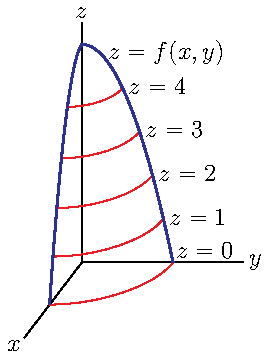
\includegraphics{dderivB.pdf}\qquad
   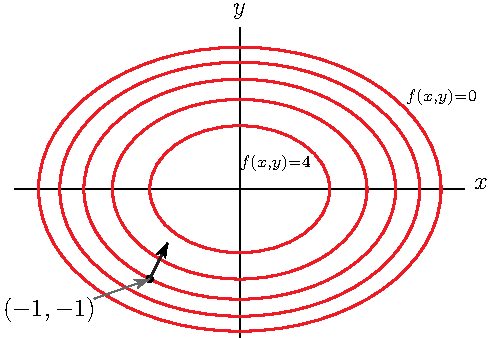
\includegraphics{dderivC.pdf}
\end{center}
\end{efig}
%\centerline{\figplace{}{-1in}{-0.3in}\hskip0.5in
%\figput{dderivC}}
\end{eg}

\begin{eg}\label{eg dir deriv D}
\noindent\textit{Problem}:
What is the rate of change of $f(x,y,z)=x^2+y^2+z^2$ at $(3,5,4)$ moving 
in the positive $x$-direction along the curve of intersection of
the surfaces $G(x,y,z)=25$ and $H(x,y,z)=0$ where
\begin{equation*}
G(x,y,z)=2x^2-y^2+2z^2 \qquad\text{and}\qquad
H(x,y,z)=x^2-y^2+z^2
\end{equation*}
\medskip
\noindent\textit{Solution}. 
As a first check note that $(3,5,4)$
really does lie on both surfaces because
\begin{alignat*}{3}
G(3,5,4)&= 2\big(3^2\big)-5^2+2\big(4^2\big) &&= 18-25+32=25  \\
H(3,5,4)&=\phantom{2*\ }3^2-5^2+\phantom{2*}4^2&&=\phantom{1}9-25+16 =0
\end{alignat*}
We compute gradients to get the normal vectors to the surfaces 
$G(x,y,z)=25$ and $H(x,y,z)=0$ at $(3,5,4)$.
\begin{alignat*}{5}
\vnabla G(3,5,4) &=\Big[4x\,\hi-2y\,\hj+4z\,\hk\Big]_{(3,5,4)}
                 &&= 12\,\hi-10\,\hj+16\,\hk 
                 &&= 2\big(6\,\hi-5\,\hj+8\,\hk\big) \\
\vnabla H(3,5,4) &=\Big[2x\,\hi-2y\,\hj+2z\,\hk\Big]_{(3,5,4)}
                 &&= 6\,\hi-10\,\hj+8\,\hk 
                 &&= 2\big(3\,\hi-5\,\hj+4\,\hk\big) 
\end{alignat*}
The direction of interest is tangent to the curve of intersection.
So the direction of interest is tangent to both surfaces and hence is
perpendicular to both gradients. Consequently one tangent vector to the 
curve at $(3,5,4)$ is
\begin{align*}
\vnabla G(3,5,4)\,\times  \vnabla H(3,5,4)
&=4\big(6\,\hi-5\,\hj+8\,\hk\big)\times\big(3\,\hi-5\,\hj+4\,\hk\big) \\
&=4\ \det\left[\begin{matrix}
             \hi & \hj & \hk \\
             6   & -5  & 8 \\
             3   & -5  & 4 
           \end{matrix}\right] \\
&= 4\ \big(20\,\hi -15\,\hk\big)
= 20\ \big(4\,\hi -3\,\hk\big)
\end{align*}
and the unit tangent vector to the curve at $(3,5,4)$ that has
positive $x$ component is 
\begin{equation*}
%\frac{20\,\hi -15\,\hk}{|20\,\hi -15\,\hk|}=
\frac{4\,\hi -3\,\hk}{|4\,\hi -3\,\hk|}
=\frac{4}{5}\,\hi -\frac{3}{5}\,\hk
\end{equation*}
The desired rate of change is
\begin{align*}
D_{\frac{4}{5}\,\hi -\frac{3}{5}\,\hj} f(3,5,4) 
   &= \vnabla f(3,5,4)\cdot\left(\frac{4}{5}\,\hi -\frac{3}{5}\,\hk\right)
   = \overbrace{\big( 6\,\hi +10\, \hj + 8\,\hk\big)}^
              {[2x\,\hi+2y\,\hj+2z\,\hk]_{(x,y,z)=(3,5,4)}}\hskip-0.15in\cdot\,  
         \left(\frac{4}{5}\,\hi -\frac{3}{5}\,\hk\right) \\
  &=0
\end{align*}
Actually, we could have known that the rate of change would be zero.
\begin{itemize}\itemindent=-0.1in
\item
Any point $(x,y,z)$ on the curve obeys both $y^2=x^2+z^2$ 
      and $2x^2-y^2+2z^2=25$. 
\item
Substituting $y^2=x^2+z^2$ into $2x^2-y^2+2z^2=25$ gives $x^2+z^2=25$. 
\item
So, at any point on the curve, $x^2+z^2=25$ and $y^2=x^2+z^2=25$ so 
that $x^2+y^2+z^2=50$. 
\item
That is, $f(x,y,z)=x^2+y^2+z^2$ takes the value 50 at every point of the curve.
\item
So of course the rate of change of $f$ along the curve is $0$.
\end{itemize}
\end{eg}

Let's change things up a little. In the next example, we are told the rates of change in two different directions. From this we are to determine the rate of change in a third direction.

\begin{eg}\label{eg dir deriv E}
\noindent\textit{Problem}:
The rate of change of a given function $f(x,y)$ at the point $P_0=(1,2)$
in the direction towards $P_1=(2,3)$ is $2\sqrt{2}$ and in the direction 
towards $P_2=(1,0)$ is $-3$. What is the rate of change of $f$ at $P_0$ 
towards the origin $P_3=(0,0)$?

\medskip
\noindent\textit{Solution}. 
We can easily determine the rate of change of $f$ at the point $P_0$
in any direction once we know the gradient $\vnabla f(1,2) =a\,\hi+b\,\hj$.
So we will first use the two given rates of change to determine $a$ and $b$,
and then we determine the rate of change towards $(0,0)$.

The two rates of change that we are given are those in the directions 
of the vectors
\begin{align*}
\overrightarrow{P_0P_1} = \llt 1,1\rgt \qquad
\overrightarrow{P_0P_2} = \llt 0,-2\rgt 
%\overrightarrow{P_0P_3} &= \llt -1,-2\rgt
\end{align*}
As you might guess, the notation $\overrightarrow{PQ}$ means the
vector whose tail is at $P$ and whose head is at $Q$.
So the given rates of change tell us that
\begin{alignat*}{5}
2\sqrt{2}&=D_{\frac{\llt 1,1\rgt}{|\llt 1,1\rgt|}} f(1,2) 
   &&= \vnabla f(1,2)\cdot\frac{\llt 1,1\rgt}{|\llt 1,1\rgt|}
   &&= \llt a,b\rgt\cdot\frac{\llt 1,1\rgt}{\sqrt{2}}
   &&=\frac{a}{\sqrt{2}} +\frac{b}{\sqrt{2}} \\
-3&=D_{\frac{\llt 0,-2\rgt}{|\llt 0,-2\rgt|}} f(1,2) 
   &&= \vnabla f(1,2)\cdot\frac{\llt 0,-2\rgt}{|\llt 0,-2\rgt|}
   &&= \llt a,b\rgt\cdot\frac{\llt 0,-2\rgt}{2}
   &&=-b 
\end{alignat*}
These two lines give us two linear equations in the two unknowns $a$ and $b$. 
The second equation directly gives us $b=3$. Substituting $b=3$ into 
the first equation gives
\begin{align*}
\frac{a}{\sqrt{2}} +\frac{3}{\sqrt{2}} = 2\sqrt{2} \implies
a+3=4 \implies
a=1
\end{align*}
A direction vector from $P_0=(1,2)$ towards $P_3=(0,0)$ is
\begin{equation*}
\overrightarrow{P_0P_3} = \llt -1,-2\rgt
\end{equation*}
and the rate of change (per unit distance) in that direction is
\begin{align*}
D_{\frac{\llt -1,-2\rgt}{|\llt -1,-2\rgt|}} f(1,2) 
   &= \vnabla f(1,2)\cdot\frac{\llt -1,-2\rgt}{|\llt -1,-2\rgt|}
    = \llt a,b\rgt\cdot\frac{\llt -1,-2\rgt}{\sqrt{5}}
    = \llt 1,3\rgt\cdot\frac{\llt -1,-2\rgt}{\sqrt{5}}
=-\frac{7}{\sqrt{5}}
\end{align*}
\end{eg}

\begin{eg}[Optional]\label{eg dir deriv F}
\noindent\textit{Problem}:
Find all points $(a,b,c)$ for which the spheres
$(x-a)^2+(y-b)^2+(z-c)^2 =1$ and $x^2+y^2+z^2=1$ intersect
orthogonally. That is, the tangent planes to the two spheres are 
to be perpendicular at each point of intersection.

\medskip
\noindent\textit{Solution}. Let $(x_0,y_0,z_0)$ be a point of intersection.
That is
\begin{align*}
(x_0-a)^2+(y_0-b)^2+(z_0-c)^2 & = 1 \\
x_0^2+y_0^2+z_0^2&=1
\end{align*}
A normal vector to $G(x,y,z)=(x-a)^2+(y-b)^2+(z-c)^2 =1$ at $(x_0,y_0,z_0)$
is
\begin{equation*}
\vN = \vnabla G(x_0,y_0,z_0) 
     = \llt 2(x_0-a)\,\hi\,,\,2(y_0-b)\,\hj\,,\,2(z_0-c)\,\hk\rgt 
\end{equation*}
A normal vector to $g(x,y,z)=x^2+y^2+z^2 =1$ at $(x_0,y_0,z_0)$
is
\begin{equation*}
\vn = \vnabla g(x_0,y_0,z_0) 
     = \llt 2x_0\,\hi\,,\,2y_0\,\hj\,,\,2z_0\,\hk\rgt 
\end{equation*}
The two tangent planes are perpendicular if and only if $\hN$ and $\hn$
are perpendicular, which is the case if and only if
\begin{equation*}
0=\hN\cdot\hn = 4x_0(x_0-a) + 4y_0(y_0-b) +4z_0(z_0-c)
\end{equation*}
or, dividing the equation by $4$,
\begin{equation*}
x_0(x_0-a) + y_0(y_0-b) +z_0(z_0-c)=0
\end{equation*}

Let's pause to take stock.
We need to find all $(a,b,c)$'s such that the statement
\begin{equation*}
(x_0,y_0,z_0)\text{ is a point of intersection of the two spheres}
\tag{S1}\end{equation*}
implies the statement
\begin{equation*}
\text{the normal vectors $\hN$ and $\hn$ are perpendicular}
\tag{S2}\end{equation*}
In equations, we need to find all $(a,b,c)$'s such that the statement
\begin{equation}
(x_0,y_0,z_0)\quad\text{obeys}\quad 
x_0^2+y_0^2+z_0^2 = 1\text{ and }(x_0-a)^2+(y_0-b)^2+(z_0-c)^2 = 1
\tag{S1}
\end{equation}
implies the statement
\begin{equation}
(x_0,y_0,z_0)\quad\text{obeys}\quad 
x_0(x_0-a) + y_0(y_0-b) +z_0(z_0-c)=0
\tag{S2}
\end{equation}
Now if we expand (S2) then we can, with a little care, massage it into something that looks more like (S1).
\begin{align*}
&x_0(x_0-a) + y_0(y_0-b) +z_0(z_0-c)
=x_0^2+y_0^2+z_0^2 -ax_0 -by_0 - cz_0 \\
&\hskip1in=\frac{1}{2}\left\{\big[x_0^2+y_0^2+z_0^2\big]
     +\big[(x_0-a)^2+(y_0-b)^2+(z_0-c)^2\big]
     -a^2-b^2-c^2\right\}
\end{align*}
If (S1) is true, then $\big[x_0^2+y_0^2+z_0^2\big]=1$
and $\big[(x_0-a)^2+(y_0-b)^2+(z_0-c)^2\big]=1$ so that
\begin{equation*}
x_0(x_0-a) + y_0(y_0-b) +z_0(z_0-c)
=\frac{1}{2}\left\{1 \ +\  1\  -a^2-b^2-c^2 \right\}
\end{equation*}
and statement (S2) is true if and only if
\begin{equation*}
a^2+b^2+c^2=2
\end{equation*}

Our conclusion is that the set of allowed points $(a,b,c)$ is the
sphere of radius $\sqrt{2}$ centred on the origin.
\end{eg}

\begin{eg}[Optional --- The gradient in polar coordinates]\label{eg:chainRuleF}
\noindent\textit{Question}:
What is the gradient of a function in polar coordinates?

\medskip
\noindent\textit{Answer}.
As was the case in Examples \ref{eg:chainRuleD} and \ref{eg:chainRuleE}, figuring 
out what the question is asking is half the battle. By Definition 
\ref{def gradient}, the gradient of a function $g(x,y)$
is the vector $\llt g_x(x,y),g_y(x,y)\rgt$. In this question we are told
that we are given some function $f(r,\theta)$ of the polar 
coordinates\footnote{Polar coordinates were defined in 
Example \ref{ex LIMtwodB}.} $r$ and $\theta$. We are supposed to convert 
this function to Cartesian  coordinates. 

This means that we are to consider the function
$$
g(x,y)=f\big(r(x,y),\theta(x,y)\big)
$$
with
\begin{align*}
r(x,y)&=\sqrt{x^2+y^2}\cr
\theta(x,y)&= \arctan\,\frac{y}{x}
\end{align*}
Then we are to compute the gradient of $g(x,y)$ and express the answer
in terms of $r$ and $\theta$. By the chain rule,
\begin{align*}
\pdiff{g}{x}
&=\pdiff{f}{r}\ \pdiff{r}{x}
           +\pdiff{f}{\theta}\  \pdiff{\theta}{x} \\
&=\pdiff{f}{r}\ \frac{1}{2}\frac{2x}{\sqrt{x^2+y^2}}
        +\pdiff{f}{\theta}\ \frac{-y/x^2}{1+(y/x)^2} \\
&=\pdiff{f}{r}\ \frac{x}{\sqrt{x^2+y^2}}
        -\pdiff{f}{\theta}\ \frac{y}{x^2+y^2} \\
&=\pdiff{f}{r}\ \frac{r\cos\theta}{r}
       -\pdiff{f}{\theta}\ \frac{r\sin\theta}{r^2} \\
\intertext{since $x=r\cos\theta$ and $y=r\sin\theta$}
&=\pdiff{f}{r}\ \cos\theta
           -\pdiff{f}{\theta}\ \frac{\sin\theta}{r}
\end{align*}
Similarly
\begin{align*}
\pdiff{g}{y}
&=\pdiff{f}{r}\ \pdiff{r}{y}
           +\pdiff{f}{\theta}\ \pdiff{\theta}{y} \\
&=\pdiff{f}{r}\ \frac{1}{2}\frac{2y}{\sqrt{x^2+y^2}}
         +\pdiff{f}{\theta}\ \frac{1/x}{1+(y/x)^2} \\
&=\pdiff{f}{r}\ \frac{y}{\sqrt{x^2+y^2}}
           +\pdiff{f}{\theta}\ \frac{x}{x^2+y^2} \\
&=\pdiff{f}{r}\ \sin\theta
     +\pdiff{f}{\theta}\ \frac{\cos\theta}{r}
\end{align*}
So
\begin{equation*}
\llt g_x,g_y\rgt= f_r\ \llt\cos\theta,\sin\theta\rgt
           +\frac{f_\theta}{r}\llt-\sin\theta,\cos\theta\rgt
\end{equation*}
or, with all the arguments written explicitly,
\begin{align*}
\llt g_x(x,y),g_y(x,y)\rgt
&=
f_r\big(r(x,y),\theta(x,y)\big)\ \llt\cos\theta(x,y)\,,\,\sin\theta(x,y)\rgt \\
&\ \ +\frac{1}{r(x,y)}f_\theta\big(r(x,y),\theta(x,y)\big)\ 
\llt-\sin\theta(x,y)\,,\,\cos\theta(x,y)\rgt
\end{align*}
\end{eg}

\section{Optional --- Solving the Wave Equation}\label{sec wave}
Many phenomena are modelled by equations that relate the rates of
change of various quantities. As rates of change are given by derivatives
the resulting equations contain derivatives and so are called
differential equations. We saw a number of such differential equations
in \S\eref{CLP101}{sec sep de} of the CLP-1 text.

In this section we consider 
\begin{equation*}
\frac{\partial^2 w}{\partial x^2}(x,t)
         -\frac{1}{c^2}\frac{\partial^2 w}{\partial t^2}(x,t)=0
\end{equation*}
This is an extremely important\footnote{If you plug ``wave equation'' into your favourite search engine you will get more than a million hits.}partial differential equation called the ``wave equation'' (in one spatial dimension)
that is used in modelling water waves, sound waves, seismic waves,
light waves and so on.
The reason that we are looking at it here is that we can use what we have just
learned to see that its solutions are waves travelling with speed $c$.

To start, we'll use gradients and the chain rule to find the solution
of the slightly simpler equation
\begin{equation*}
\pdiff{w}{x}(x,t)-\frac{1}{c}\pdiff{w}{t}(x,t)=0
\end{equation*}
By way of motivation for what will follow, note that
\begin{itemize} 
\item 
we can rewrite the above equation as
\begin{equation*}
\llt 1\,,\,-\frac{1}{c}\rgt\cdot \vnabla w(x,t) =0
\end{equation*}
\item
This equation tells that the gradient of any solution $w(x,t)$ must always be 
perpendicular to the constant vector $\big< 1\,,\,-\frac{1}{c}\big>$.
\item
A vector $\llt a,b\rgt$ is perpendicular to $\big< 1\,,\,-\frac{1}{c}\big>$
if and only if 
\begin{align*}
\llt a,b\rgt \cdot \llt 1\,,\,-\frac{1}{c}\rgt =0
&\iff a-\frac{b}{c} = 0
\iff b=ac
\iff \llt a,b\rgt =a \llt 1,c\rgt
\end{align*}
That is, a vector is perpendicular to $\big< 1\,,\,-\frac{1}{c}\big>$
if and only if it is parallel to $\llt 1,c\rgt$.
\item
Thus the gradient of any solution $w(x,t)$ must always be parallel 
to the constant vector $\llt 1\,,\,c\rgt$. 
\item 
Recall that one of our implications following Definition 
\ref{def dri deriv} is that the gradient of $w(x,t)$ must always be 
perpendicular to the level curves of $w$. 
\item
So the level curves of $w(x,t)$ are always perpendicular to the
constant vector $\big< 1\,,\,c\big>$. They must be straight lines
with equations of the form
\begin{equation*}
\llt 1\,,\,c\rgt\cdot\llt x-x_0\,,\,t-t_0\rgt =0\qquad\text{or}\qquad
x+ct=u\quad\text{with $u$ a constant}
\end{equation*}
\begin{nfig}
\begin{center}
   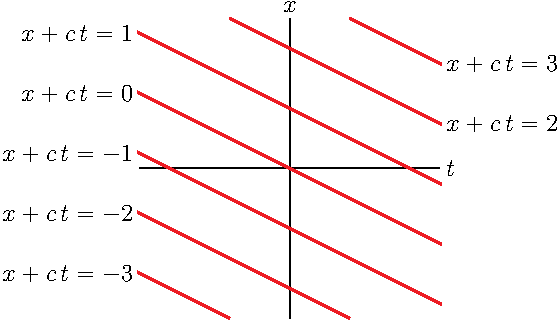
\includegraphics{level.pdf}
\end{center}
\end{nfig}

\item
That is, for each constant $u$, $w(x,t)$ takes the same value at each point
of the straight line $x+ct=u$. Call that value $U(u)$. So
$w(x,t)=U(u)=U(x+ct)$ for some function $U$.
\end{itemize}\noindent
This solution represents a wave packet moving to the left with speed $c$. 
You can see this by observing that all points $(x,t)$ in space-time for 
which $x+ct$ takes the same fixed value, say $z$, have the same value 
of $U(x+ct)$, namely $U(z)$. So if you move so that your position at 
time $t$ is $x=z-ct$  (i.e. move the left with speed $c$) you always 
see the same value of $w$.
The figure below illustrates this. It contains the graphs of $U(x)$, $U(x+c)
=U(x+ct)\big|_{t=1}$ and  $U(x+2c)=U(x+ct)\big|_{t=2}$ for a bump shaped
$U(x)$. In the figure the location of the tick $z$ on the
$x$-axis was chosen so that so that $U(z)=\max_x U(x)$.

\begin{efig}
\begin{center}
   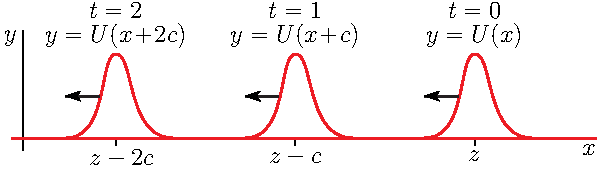
\includegraphics{bumpLeft.pdf}
\end{center}
\end{efig}

The above argument that lead to the solution $w(x,t)=U(x+ct)$
was somewhat handwavy. But we can easily turn it into
a much tighter argument by simply changing variables from $(x,y)$
to $(u,v)$ with $u=x+ct$. It doesn't much matter what we choose
(within reason) for the new variable $v$. Let's take $v=x-ct$.
Then $x=\frac{u+v}{2}$ and $t=\frac{u-v}{2c}$ and it is easy to translate
back and forth between $x,t$ and $u,v$. 

Now define the function $W(u,v)$ by
\begin{equation*}
w(x,t) = W(x+ct\,,\,x-ct)
\end{equation*} 
By the chain rule
\begin{align*}
\pdiff{w}{x}(x,t)
&=\pdiff{}{x}\big[W(x+ct\,,\,x-ct) \big] \\
&= \pdiff{W}{u}(x+ct\,,\,x-ct)\pdiff{}{x}(x+ct) 
  + \pdiff{W}{v}(x+ct\,,\,x-ct) \pdiff{}{x}(x-ct)  \\
&= \pdiff{W}{u}(x+ct\,,\,x-ct) + \pdiff{W}{v}(x+ct\,,\,x-ct)  
\end{align*}
and
\begin{align*}
\pdiff{w}{t}(x,t)
&=\pdiff{}{t}\big[W(x+ct\,,\,x-ct) \big] \\
&= \pdiff{W}{u}(x+ct\,,\,x-ct)\pdiff{}{t}(x+ct) 
  + \pdiff{W}{v}(x+ct\,,\,x-ct) \pdiff{}{t}(x-ct)  \\
&= \pdiff{W}{u}(x+ct\,,\,x-ct)\times c 
             + \pdiff{W}{v}(x+ct\,,\,x-ct)\times(-c)  
\end{align*}
Subtracting $\frac{1}{c}$ times the second equation from
the first equation gives 
\begin{equation*}
\pdiff{w}{x}(x,t)-\frac{1}{c}\pdiff{w}{t}(x,t)
= 2 \pdiff{W}{v}(x+ct\,,\,x-ct)
\end{equation*}
So 
\begin{align*}
&\text{$w(x,t)$ obeys the equation 
$\pdiff{w}{x}(x,t)-\frac{1}{c}\pdiff{w}{t}(x,t)=0$ for all $x$ and $t$}\\
\intertext{if and only if }
&\text{$W(u,v)$ obeys the equation  $\pdiff{W}{v}(x+ct\,,\,x-ct)=0$
for all $x$ and $t$,}\\
\intertext{which, substituting in $x=\frac{u+v}{2}$ and $t=\frac{u-v}{2c}$,  
                  is the case if and only if} 
&\text{$W(u,v)$ obeys the equation  $\pdiff{W}{v}(u\,,\,v)=0$
for all $u$ and $v$}
\end{align*}
The equation $\pdiff{W}{v}(u\,,\,v)=0$ means that $W(u,v)$ is independent of
$v$, so that $W(u,v)$ is of the form $W(u,v)=U(u)$, for some function $U$,
and, so finally,
\begin{equation*}
w(x,t) = W(x+ct\,,\,x-ct) = U(x+ct)
\end{equation*}

Now that we have solved our toy equation, let's move on to the 1d
wave equation.

\begin{eg}[Wave Equation]
We'll now expand the above argument to find the general solution 
to 
\begin{equation*}
\frac{\partial^2 w}{\partial x^2}(x,t)
         -\frac{1}{c^2}\frac{\partial^2 w}{\partial t^2}(x,t)=0
\end{equation*}

 We'll again make the change of variables from $(x,y)$
to $(u,v)$ with $u=x+ct$ and $v=x-ct$ and again define
the function $W(u,v)$ by
\begin{equation*}
w(x,t) = W(x+ct\,,\,x-ct)
\end{equation*} 
By the chain rule, we still have
\begin{alignat*}{3}
\pdiff{w}{x}(x,t)
&=\pdiff{}{x}\big[W(x+ct\,,\,x-ct) \big]
&&= \pdiff{W}{u}(x+ct\,,\,x-ct) + \pdiff{W}{v}(x+ct\,,\,x-ct)  \\
\pdiff{w}{t}(x,t)
&=\pdiff{}{t}\big[W(x+ct\,,\,x-ct) \big]
&&= \pdiff{W}{u}(x+ct\,,\,x-ct)\times c 
             + \pdiff{W}{v}(x+ct\,,\,x-ct)\times(-c)  
\end{alignat*}
We now need to differentiate a second time. Write
$W_1(u,v)=\pdiff{W}{u}(u,v)$ and $W_2(u,v)=\pdiff{W}{v}(u,v)$
so that
\begin{align*}
\pdiff{w}{x}(x,t)
&= W_1(x+ct\,,\,x-ct) + W_2(x+ct\,,\,x-ct)  \\
\pdiff{w}{t}(x,t)
&= c\,W_1(x+ct\,,\,x-ct) -c\,W_2(x+ct\,,\,x-ct)
\end{align*}
Using the chain rule again
\begin{alignat*}{3}
\frac{\partial^2 w}{\partial x^2}(x,t)
&=\pdiff{}{x}\left[\pdiff{w}{x}(x,t)\right] \\
&=\pdiff{}{x}\left[W_1(x+ct\,,\,x-ct)\right]
  &&+ \pdiff{}{x}\left[W_2(x+ct\,,\,x-ct)\right] \\
&=\pdiff{W_1}{u}  
     \ +\  \pdiff{W_1}{v}
   &&+ \pdiff{W_2}{u}
     \ +\  \pdiff{W_2}{v}  \\
&=\frac{\partial^2 W}{\partial u^2}  
     \ +\  \frac{\partial^2\ W}{\partial v\,\partial u}
   &&+ \frac{\partial^2\ W}{\partial u\ \partial v}
     \ +\  \frac{\partial^2 W}{\partial v^2}  \\
%%
\frac{\partial^2 w}{\partial t^2}(x,t)
&=\pdiff{}{t}\left[\pdiff{w}{t}(x,t)\right] \\
&=c\pdiff{}{t}\left[W_1(x+ct\,,\,x-ct)\right]
  &&-c \pdiff{}{t}\left[W_2(x+ct\,,\,x-ct)\right] \\
&=c^2\pdiff{W_1}{u}  
     \ -\  c^2\pdiff{W_1}{v}
   && -c^2\pdiff{W_2}{u}
     \ +\  c^2\pdiff{W_2}{v}  \\
&=c^2\frac{\partial^2 W}{\partial u^2}  
     \ -\  c^2\frac{\partial^2 W}{\partial v\partial u}
    && - c^2\frac{\partial^2 W}{\partial u\partial v}
     \ +\  c^2\frac{\partial^2 W}{\partial v^2}  
\end{alignat*}
with all of the functions on the right hand sides having arguments
$(x+ct\,,\,x-ct)$. So, subtracting $\frac{1}{c^2}$ times the second from the
first, we get
\begin{align*}
\frac{\partial^2 w}{\partial x^2}(x,t)
         -\frac{1}{c^2}\frac{\partial^2 w}{\partial t^2}(x,t)
&=4 \frac{\partial^2 W}{\partial u\partial v}(x+ct\,,\,x-ct)
\end{align*}
and $w(x,t)$ obeys $\frac{\partial^2 w}{\partial x^2}(x,t)
         -\frac{1}{c^2}\frac{\partial^2 w}{\partial t^2}(x,t)=0$
for all $x$ and $t$ if and only if 
\begin{equation*}
\frac{\partial^2 W}{\partial u\partial v}(u\,,\,v)=0
\end{equation*}
for all $u$ and $v$. 

\begin{itemize}
\item
This tells us that the $u$-derivative of $\pdiff{W}{v}$ is zero, 
so that $\pdiff{W}{v}$ is independent of $u$.
That is $\pdiff{W}{v}(u,v) = \widetilde V(v)$ for some function $\tilde V$.
The reason that we have called it $\widetilde V$ instead of $V$ with become
evident shortly.
\item
Recall that to apply $\pdiff{}{v}$, you treat $u$ as a constant
and differentiate with respect to $v$. 
\item 
So $\pdiff{W}{v}(u,v) = \widetilde V(v)$ says that, when $u$ is thought 
of as a constant, $W$ is an antiderivative of $\widetilde V$. 
\item
That is, $W(u,v) = \int \tilde V(v)\,\dee{v} +U$,
with $U$ being an arbitrary constant. As $u$ is being thought of as 
a constant, $U$ is allowed to depend on $u$. 
%To check that 
%this $W(u,v)$ obeys $\pdiff{W}{v}(u,v) = \widetilde V(v)$, just
%differentiate both sides of $W(u,v) = \int \tilde V(v)\,\dee{v} +U$.
\end{itemize}\noindent
So, denoting by $V$ any antiderivative of $\tilde V$, we can write
our solution in a very neat form.
\begin{equation*}
W(u,v) = U(u) + V(v)
\end{equation*}
and the function we want is\footnote{This is known as d'Alembert's form
of the solution. It is named after Jean le Rond d'Alembert, 1717--1783,
who was a French mathematician, physicist, philosopher and music
theorist.}
\begin{equation*}
w(x,t) = W(x+ct\,,\,x-ct)
       = U(x+ct) + V(x-ct)
\end{equation*}
As we saw above $U(x+ct)$ represents a wave packet moving to the 
left with speed $c$. Similarly, $V(x-ct)$ represents a wave packet 
moving to the right with speed $c$.

Notice that $w(x,t) = U(x+ct) + V(x-ct)$ is a solution regardless of what
$U$ and $V$ are. The differential equation cannot tell us what $U$ and $V$
are. To determine them, we need more information about the system ---
usually in the form of initial conditions, like $w(x,0)=\cdots$
and $\pdiff{w}{t}(x,0)=\cdots$. General techniques for solving 
partial differential equations lie beyond this text --- but definitely
require a good understanding of multivariable calculus. A good reason to keep on reading! 

\end{eg}

%%%%%%%%%%%%%%%%%%%%%%%%%%%%%%%%%%%%%%%%%%%%%%%%%55
\subsection{Really Optional --- Derivation of the Wave Equation}
      \label{sec wave deriv}

In this section we derive the wave equation 
\begin{equation*}
\frac{\partial^2 w}{\partial x^2}(x,t)
         -\frac{1}{c^2}\frac{\partial^2 w}{\partial t^2}(x,t)=0
\end{equation*}
in one application. To be precise, we apply Newton's law to an elastic 
string, and conclude that small amplitude transverse vibrations of the 
string obey the wave equation. 

Here is a sketch of a tiny element of the string.
\begin{center}
\begin{efig}
     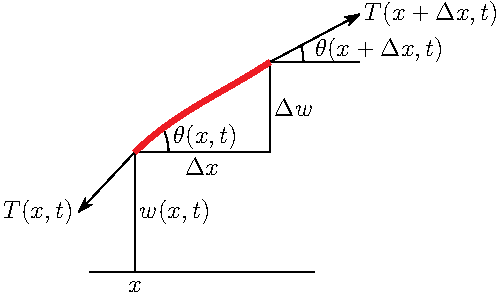
\includegraphics{string_elmnt.pdf}
\end{efig}
\end{center}
The basic notation that we will use (most of which appears in the sketch) is
\begin{align*}
w(x,t) &= \text{vertical displacement of the string from the $x$ axis at 
position $x$ and time $t$} \\
\theta(x,t) &= \text{angle between the string and a horizontal line at 
position $x$ and time $t$} \\
T(x,t) &= \text{tension in the string at position $x$ and time $t$} \\
\rho(x) &= \text{mass density (per unit length) of the string at position $x$}
\end{align*}
The forces acting on the tiny element of string at time $t$ are 
\begin{enumerate}[(a)]
\item 
tension pulling to the right, which has magnitude $T(x+\De x,t)$ and
acts at an angle $\theta(x+\De x,t)$ above horizontal 
\item
tension pulling to the left, which has magnitude $T(x,t)$ and 
acts at an angle $\theta(x,t)$ below horizontal and, possibly, 
\item
various external forces, like
gravity. We shall assume that all of the external forces act vertically
and we shall denote by $F(x,t)\De x$ the net magnitude of the external force
acting on the element of string. 
\end{enumerate}
The length of the element of string is essentially $\sqrt{\De x^2+\De w^2}$
so that the mass of the element of string is essentially
$\rho(x)\sqrt{\De x^2+\De w^2}$ and the
vertical component of Newton's law $\vF =m\va$ says that
\begin{equation*}
\rho(x)\,\sqrt{\De x^2+\De w^2}\,
\frac{\partial^2 w}{\partial\, t^2}(x,t)
=T(x+\De x,t)\sin\theta(x+\De x,t)-T(x,t)\sin\theta(x,t)+F(x,t)\De x
\end{equation*}
Dividing by $\De x$ and taking the limit as $\De x\rightarrow 0$ gives
\begin{align*}
\rho(x)\,\sqrt{1+\left(\frac{\partial w}{\partial x}\right)^2}\,
\frac{\partial^2 w}{\partial\, t^2}(x,t)
&=\frac{\partial \hfill}{\partial x}\big[T(x,t)\sin\theta(x,t)\big]+F(x,t) \\
&=\frac{\partial T}{\partial x}(x,t)\sin\theta(x,t)
+T(x,t)\cos\theta(x,t)\,\frac{\partial \theta}{\partial x}(x,t)
+F(x,t)
\tag{E1}\end{align*}
We can dispose of all the $\theta$'s by observing from the figure above that
\begin{equation*}
\tan\theta(x,t)=\lim_{\De x\rightarrow 0}\frac{\De w}{\De x}
=\frac{\partial w}{\partial x}(x,t)
\end{equation*}
which implies, using the figure on the right below, that
\begin{align*}
\sin \theta(x,t)&= \frac{\frac{\partial w}{\partial x}(x,t)}
{\sqrt{1+\big(\frac{\partial w}{\partial x}(x,t)\big)^2}} &
\cos \theta(x,t)&= \frac{1}
{\sqrt{1+\big(\frac{\partial w}{\partial x}(x,t)\big)^2}} &
\raisebox{-1.3\height}[0pt][0pt]{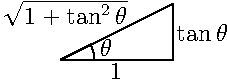
\includegraphics{triangleString.pdf}} \\
\theta(x,t)&=\arctan\frac{\partial w}{\partial x}(x,t) &
\frac{\partial \theta}{\partial x}(x,t)
&=\frac{\frac{\partial^2 w}{\partial x^2}(x,t)}
{1+\big(\frac{\partial w}{\partial x}(x,t)\big)^2}
\end{align*}

Substituting these formulae into (E1) give a horrendous mess. However,
we can get considerable simplification by looking only at small vibrations.
By a small vibration, we mean that $|\theta(x,t)|\ll 1$ for all $x$ and $t$.
This implies that $|\tan\theta(x,t)|\ll 1$, hence that 
$\big|\frac{\partial w}{\partial x}(x,t)\big|\ll 1$ and hence that
\begin{equation*}
\sqrt{1+\left(\frac{\partial w}{\partial x}\right)^2}\approx 1\qquad
\sin \theta(x,t)\approx \frac{\partial w}{\partial x}(x,t) \qquad
\cos \theta(x,t)\approx 1 \qquad
\frac{\partial \theta}{\partial x}(x,t)
\approx\frac{\partial^2 w}{\partial x^2}(x,t)
\tag{E2}\end{equation*}
Substituting these into equation (E1) give
\begin{equation*}
\rho(x)\frac{\partial^2 w}{\partial\, t^2}(x,t)
=\frac{\partial T}{\partial x}(x,t)\frac{\partial w}{\partial x}(x,t)
+T(x,t)\,\frac{\partial^2 w}{\partial x^2}(x,t)
+F(x,t)
\tag{E3}\end{equation*}
which is indeed relatively simple, but still exhibits a problem. This is
one equation in the two unknowns $w$ and $T$. 

Fortunately there is a second
equation lurking in the background, that we haven't used yet. Namely, the 
horizontal component of Newton's law of motion. As a second simplification,
we assume that there are only transverse vibrations. That is, our tiny 
string element moves only vertically. Then the net horizontal force on 
it must be zero. That is,
\begin{equation*}
T(x+\De x,t)\cos\theta(x+\De x,t)-T(x,t)\cos\theta(x,t)=0
\end{equation*}
Dividing by $\De x$ and taking the limit as $\De x$ tends to zero gives
\begin{equation*}
\frac{\partial \hfill}{\partial x}\big[T(x,t)\cos\theta(x,t)\big]=0
\end{equation*}
Thus $T(x,t)\cos\theta(x,t)$ is independent of $x$.
For small amplitude vibrations, $\cos\theta$ is very close to one, for all
$x$. So $T$ is a function of $t$ only, which is determined by how hard you are
pulling on the ends of the string at time $t$. So for small, transverse
vibrations, (E3) simplifies further to
\begin{equation*}
\rho(x)\frac{\partial^2 w}{\partial\, t^2}(x,t)
=T(t)\,\frac{\partial^2 w}{\partial x^2}(x,t)
+F(x,t)
\tag{E4}\end{equation*}
In the event that the string density $\rho$ is a constant, independent
of $x$, the string tension $T(t)$ is a constant independent of $t$
(in other words you are not continually playing with the tuning pegs)
and there are no external forces $F$ we end up with the wave equation
\begin{equation*}
\frac{\partial^2 w}{\partial\, t^2}(x,t)
=c^2\,\frac{\partial^2 w}{\partial x^2}(x,t)
\qquad
\text{where}\qquad
c=\sqrt{\frac{T}{\rho}}
\end{equation*}
as desired.

The equation that is called the wave equation has built into it a
lot of approximations. By going through the derivation, we have 
seen what those approximations are, and we can get some idea as to when they
are applicable.

%%%%%%%%%%%%%%%%%%%%%%%%%%%%%%%%%%%%%5
\section{Maximum and Minimum Values}\label{sec max}

One of the core topics in single variable calculus courses 
is finding the maxima and minima of functions of one variable.
We'll now extend that discussion to functions of more than one 
variable\footnote{Life is not (always) one-dimensional and sometimes we have to embrace it.}. Rather than leaping into the deep end, we'll not be too 
ambitious and concentrate on functions of two variables. That being said, 
many of the techniques work more generally.
To start, we have the following natural extensions to some familiar
definitions.

\begin{defn}\label{def local max min}
Let the function $f(x,y)$ be defined for all $(x,y)$ in some
subset $R$ of $\bbbr^2$. Let $(a,b)$ be a point in $R$.
\begin{itemize}
\item
$(a,b)$ is a \emph{local maximum} of $f(x,y)$ if
$f(x,y)\le f(a,b)$ for all $(x,y)$ close to $(a,b)$.
More precisely, $(a,b)$ is a local maximum of $f(x,y)$ if there is 
an $r>0$ such that $f(x,y)\le f(a,b)$ for 
all points $(x,y)$ within a distance $r$ of $(a,b)$. 

\item
$(a,b)$ is a \emph{local minimum} of $f(x,y)$ if
$f(x,y)\ge f(a,b)$ for all $(x,y)$ close to $(a,b)$.

\item 
Local maximum and minimum values are also called extremal values.

\item
$(a,b)$ is an \emph{absolute maximum} or
\emph{global maximum} of $f(x,y)$ if
$f(x,y)\le f(a,b)$ for all $(x,y)$ in $R$.

\item
$(a,b)$ is an \emph{absolute minimum} or
\emph{global minimum} of $f(x,y)$ if
$f(x,y)\ge f(a,b)$ for all $(x,y)$ in $R$.
\end{itemize}
\end{defn}

\subsection*{Local Maxima and Minima}
One of the first things you did when you were developing the techniques
used to find the maximum and minimum values of $f(x)$ was ask
yourself\footnote{Or perhaps your instructor asked you.}
\begin{description}
\item[\hskip0.25in] 
Suppose that the largest value of $f(x)$ is $f(a)$. 
What does that tell us about $a$?
\end{description}
After a little thought you answered
\begin{description}
\item[\hskip0.25in] 
If the largest value of $f(x)$ is $f(a)$
and $f$ is differentiable at $a$, then $f'(a)=0$.
\end{description}
\begin{nfig}
\begin{center}
   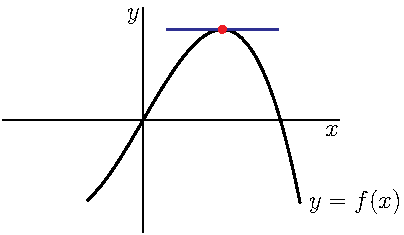
\includegraphics{localMaxA.pdf}
\end{center}
\end{nfig}
Let's recall why that's true. Suppose that the largest value of $f(x)$
is $f(a)$. Then for all $h>0$,
\begin{equation*}
f(a+h)\le f(a)
\implies f(a+h)-f(a)\le 0
\implies \frac{f(a+h)-f(a)}{h}\le 0\quad\text{if $h>0$}
\end{equation*}
Taking the limit $h\rightarrow 0$ tells us that $f'(a)\le 0$.
Similarly,  for all $h<0$,
\begin{equation*}
f(a+h)\le f(a)
\implies f(a+h)-f(a)\le 0
\implies \frac{f(a+h)-f(a)}{h}\ge 0\quad\text{if $h<0$}
\end{equation*}
Taking the limit $h\rightarrow 0$ now tells us that $f'(a)\ge 0$.
So we have both $f'(a)\ge 0$ and $f'(a)\le 0$ which forces $f'(a)=0$.

You also observed at the time that for this argument to work, you only
need $f(x)\le f(a)$ for all $x$'s close to $a$, not necessarily for all
$x$'s in the whole world. (In the above inequalities, we only used
$f(a+h)$ with $h$ small.) Since we care only about $f(x)$ for $x$ near $a$, 
we can refine the above statement.
\begin{description}
\item[\hskip0.25in] 
If $f(a)$ is a local maximum for $f(x)$
and $f$ is differentiable at $a$, then $f'(a)=0$.
\end{description}
Precisely the same reasoning applies to minima.
\begin{description}
\item[\hskip0.25in] 
If $f(a)$ is a local minimum for $f(x)$
and $f$ is differentiable at $a$, then $f'(a)=0$.
\end{description}

Let's use the ideas of the above discourse to extend the study of
local maxima and local minima to functions of more than one variable.
Suppose that the function $f(x,y)$ is defined for all $(x,y)$ in some
subset $R$ of $\bbbr^2$, that $(a,b)$ is point of $R$ that is not on the boundary of $R$, and that $f$ has a local maximum at $(a,b)$.
See the figure below.
\begin{efig}
\begin{center}
   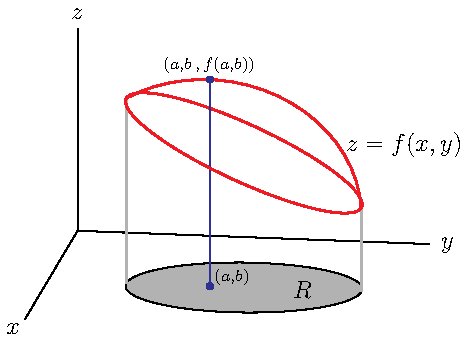
\includegraphics{max.pdf}
\end{center}
\end{efig}
Then the function $f(x,y)$ must decrease in value as $(x,y)$ moves away from $(a,b)$ in \emph{any} direction. No matter which direction $\vd$ we choose,
the directional derivative of $f$ at $(a,b)$ in direction $\vd$ 
must be zero or smaller. Writing this in mathematical symbols, we get
\begin{align*}
D_\vd f(a,b) = \vnabla f(a,b)\cdot\frac{\vd}{|\vd|}\le 0
\end{align*}
And the directional derivative of $f$ at $(a,b)$ in the direction $-\vd$ 
also must be zero or negative.
\begin{align*}
D_{-\vd} f(a,b) = \vnabla f(a,b)\cdot\frac{-\vd}{|\vd|}\le 0
\quad\text{which implies that}\quad \vnabla f(a,b)\cdot\frac{\vd}{|\vd|}\ge 0
\end{align*}
As $\vnabla f(a,b)\cdot\frac{\vd}{|\vd|}$ must be both positive (or zero)
and negative (or zero) at the same time, it must be zero. 
In particular, choosing $\vd=\hi$ forces the $x$ component of 
$\vnabla f(a,b)$ to be zero, and  choosing 
$\vd=\hj$ forces the $y$ component of $\vnabla f(a,b)$ to be zero.
We have thus shown that  $\vnabla f(a,b)=\vZero$. The same argument
shows that $\vnabla f(a,b)=\vZero$ when $(a,b)$ is a local minimum too.
This is an important and useful result, so let's theoremise it.

\begin{theorem}\label{thm stationary point}
Let the function $f(x,y)$ be defined for all $(x,y)$ in some subset $R$ 
of $\bbbr^2$. Assume that
\begin{itemize}\itemsep1pt \parskip0pt \parsep0pt
\item[$\circ$]
$(a,b)$ is a point of $R$ that is not on the boundary of $R$ and
\item[$\circ$]
$(a,b)$ is a local maximum or local minimum of $f$ and that
\item[$\circ$]
the partial derivatives of $f$ exist at $(a,b)$.
\end{itemize}
Then
\begin{equation*}
\vnabla f(a,b) = \vZero.
\end{equation*}
\end{theorem}

\begin{defn}\label{def critical point} 
Let $f(x,y)$ be a function and let $(a,b)$ be a point in its domain. Then
\begin{itemize}
 \item if $\vnabla f(a,b)$ exists and is zero we call $(a,b)$ 
a critical point (or a stationary point) of the function, and
 \item if $\vnabla f(a,b)$ does not exist then we call $(a,b)$ 
a singular point of the  function.
\end{itemize}
\end{defn}

\begin{warning}\label{warn critical point} 
Note that some people (and texts) combine both of these cases and call 
$(a,b)$ a critical point when either the gradient is zero or does not exist. 
\end{warning}

\begin{warning}\label{warn saddle} 
Theorem \ref{thm stationary point} tells us that every local maximum 
or minimum (in the interior of the domain of a function whose partial derivatives exist) 
is a critical point.  Beware that it does \emph{not}\footnote{A very common 
error of logic that people make is ``Affirming the consequent''. 
``If P then Q'' is true, does not imply that ``If Q then P'' is true . 
The statement ``If he is Shakespeare then he is dead'' is true. 
But concluding from ``That man is dead'' that ``He must be Shakespeare''
is just silly. 
%Or you may have also seen  someone use this reasoning: ``If a person 
%is a genius before their time then they are  misunderstood.'' ``I am misunderstood'' ``So I must be a genius before my time.''.
} 
tell us that every critical point is either a local maximum or a local minimum. 
\end{warning}


In fact, we shall see later\footnote{And you also saw, for example in
Example 3.6.4 of the CLP-1 text, that critical points that are also
inflection points are neither local maxima nor local minima.}, 
in Examples \ref{eg maxminA} and 
\ref{eg maxminC}, critical points that are neither local maxima nor a local minima. None-the-less, 
Theorem \ref{thm stationary point} is very useful because often functions have
only a small number of critical points. To find local maxima and minima
of such functions, we only need to consider its critical and singular
points. We'll return later to the question of how to tell if a 
critical point is a local maximum, local minimum or neither. For now, 
we'll just practice finding critical points. 

\begin{eg}[$f(x,y)=x^2-2xy+2y^2+2x-6y+12$]\label{eg:MXMNlocalA}
Find all critical points of $f(x,y)=x^2-2xy+2y^2+2x-6y+12$.

\soln
To find the critical points, we need to find the gradient. To find the 
gradient we need to find the first order partial derivatives.
So, as a preliminary calculation, we find the two first order
partial derivatives of $f(x,y)$.
\begin{align*}
f_x(x,y)&= 2x-2y+2 \\
f_y(x,y)&= -2x+4y-6 
\end{align*}
So the critical points are the solutions of the pair of equations
\begin{equation*}
2x-2y+2=0\qquad -2x+4y-6=0
\end{equation*} 
or equivalently (dividing by two and moving the constants to the 
right hand side)
\begin{subequations}\label{eq:MXMNlocalA}
\begin{align*}
x-y&=-1 \tag{E1}\\
-x+2y&=3 \tag{E2}
\end{align*}
\end{subequations}
This is a system of two equations in two unknowns ($x$ and $y$).
One strategy for solving system like this is to 
\begin{itemize}
\item First use one of the equations to solve for one of the unknowns
in terms of the other unknown. For example, (E1) tells
us that $y= x+1$. This expresses $y$ in terms of $x$. We say that we have
solved for $y$ in terms of $x$.

\item Then substitute the result, $y= x+1$ in our case, into the
other equation, (E2). In our case, this gives
\begin{equation*}
-x+2(x+1)=3
\iff x+2=3
\iff x=1
\end{equation*} 

\item We have now found that $x=1$, $y=x+1=2$ is the only solution. So
the only critical point is $(1,2)$. Of course it only takes a moment to
verify that $\vnabla f(1,2) =\llt 0,0\rgt$. It is a good idea to do this
as a simple check of our work.  

\end{itemize}
An alternative strategy for solving a system of two equations in two unknowns,
like (E1) and (E2), is to 

\begin{itemize}
\item add equations (E1) and (E2)
together. This gives 
\begin{equation*}
(E1) + (E2):\ \ \ 
 (1-1)x+(-1+2)y = -1+3
\iff y=2
\end{equation*}
The point here is that adding equations (E1) and 
(E2) together eliminates the unknown $x$, leaving us with
one equation in the unknown $y$, which is easily solved. For other
systems of equations you might have to multiply the equations by some numbers
before adding them together.

\item We now know that $y=2$. Substituting it into (E1)
gives us 
\begin{equation*}
x-2=-1
\implies x=1
\end{equation*}

\item Once again (thankfully) we have found that the only critical point is $(1,2)$.
\end{itemize}

\end{eg}
This was pretty easy because we only had to solve linear equations, which
in turn was a consequence of the fact that $f(x,y)$ was a polynomial of degree 
two. Here is an example with some slightly more challenging algebra.


\goodbreak


\begin{eg}[$f(x,y)=2x^3 - 6xy + y^2 +4y $]\label{eg:MXMNlocalB}
Find all critical points of $f(x,y)=2x^3 - 6xy + y^2 +4y $.

\soln 
As in the last example, we need to find where the gradient is zero,
and to find the gradient we need the first order partial derivatives.
\begin{equation*}
f_x=6x^2-6y   \qquad
f_y=-6x+2y+4 
\end{equation*}
So the critical points are the solutions of
\begin{equation*}
6x^2-6y=0   \qquad
-6x+2y+4 = 0
\end{equation*}
We can rewrite the first equation as $y=x^2$, which expresses $y$ as a 
function of $x$. We can then substitute $y=x^2$ into the second equation,
giving
\begin{align*}
-6x+2y+4 = 0
&\iff -6x+2x^2+4 = 0
\iff x^2-3x+2=0 
\iff (x-1)(x-2)=0 \\
&\iff x=1\text{ or }2 
\end{align*}
When $x=1$, $y=1^2=1$ and when $x=2$, $y=2^2=4$.
So, there are two critical points: $(1,1),\ (2,4)$.

Alternatively, we could have also used the second equation to write $y=3x-2$,
and then substituted that into the first equation to get
\begin{equation*}
6x^2-6(3x-2) =0
\iff x^2-3x+2=0
\end{equation*}
just as above.

\end{eg}

And here is an example for which the algebra requires a bit more thought.

\begin{eg}[$f(x,y) = xy(5x+y-15)$]\label{eg:MXMNlocalC}
Find all critical points of $f(x,y)=xy(5x+y-15) $.


\soln 
The first order partial derivatives of $f(x,y)=xy(5x+y-15)$ are
\begin{alignat*}{3}
f_x(x,y)
&\ =\ y(5x+y-15)+xy(5)
&&\ =\ y(5x+y-15)+y(5x)
&\ =\  y(10x+y-15)
\\
f_y(x,y)
&\ =\ x(5x+y-15)+xy(1)
&&\ =\ x(5x+y-15)+ x(y)
&\ =\ x(5x+2y-15)
\end{alignat*}
The critical points are the solutions of $f_x(x,y)=f_y(x,y)=0$.
That is, we need to find all $x,y$ that satisfy the pair of equations
\begin{align*}
         y(10x+y-15)&=0\tag{E1} \\
         x(5x+2y-15)&=0\tag{E2}
\end{align*}
The first equation, $y(10x+y-15)=0$, is satisfied if at least one of the
two factors $y$, $(10x+y-15)$ is zero. So the first equation is satisfied 
if at least one of the two equations
\begin{subequations}
\begin{align*}
y&=0 \tag{E1a}\\
10x+y&=15 \tag{E1b}
\end{align*}
\end{subequations}
is satisfied.
The second equation, $x(5x+2y-15)=0$, is satisfied if at least one of the two
factors $x$, $(5x+2y-15)$ is zero. So the second equation is satisfied 
if at least one of the two equations
\begin{subequations}
\begin{align*}
x&=0 \tag{E2a}\\
5x+2y&=15 \tag{E2b}
\end{align*}
\end{subequations}
is satisfied.

So both critical point equations (E1) and (E2) are satisfied
if and only if at least one of (E1a), (E1b) is satisfied
and in addition at least one of (E2a), (E2b) is satisfied.
So both critical point equations (E1) and (E2) are satisfied
if and only if at least one of the following four possibilities hold.
\begin{itemize}
\item 
(E1a) and (E2a) are satisfied
if and only if $x=y=0$
\item 
(E1a) and (E2b) are satisfied
if and only if $y=0,\ 5x+2y=15 \iff y=0,\ 5x=15$
\item 
(E1b) and (E2a) are satisfied
if and only if $10x+y=15,\ x=0 \iff y=15,\ x=0$
\item 
(E1b) and (E2b) are satisfied
if and only if $10x+y=15,\ 5x+2y=15$. We can use, for example, the second
of these equations to solve for $x$ in terms of $y$: $x =\frac{1}{5}(15-2y)$.
When we substitute this into the first equation we get $2(15-2y)+y=15$,
which we can solve for $y$. This gives $-3y=15-30$ or $y=5$ and then
$x=\frac{1}{5}(15-2\times 5)=1$.
\end{itemize}
In conclusion, the critical points are $(0,0)$, $(3,0)$, $(0,15)$ and
$(1,5)$.

A more compact way to write what we have just done is
\begin{alignat*}{3}
&           &f_x(x,y)=0\quad\qquad 
            & \text{and}\qquad 
            & f_y(x,y)=0\quad \\
& \iff\qquad          &y(10x+y-15)=0\quad\qquad 
            & \text{and}\qquad 
            & x(5x+2y-15)=0\quad \\
&\iff\qquad & \big\{y=0\text{\ \  or\ \  }10x+y=15\big\}\qquad 
            & \text{and}\qquad
            &\big\{x=0\text{\ \ or\ \ }5x+2y=15\big\}\\
&\iff\qquad & \big\{y=0,\ x=0\big\}\text{ or }
       \big\{y=0,\ 5x+2y=15\big\}\text{ or }
       \big\{10x+y=15,\ x=0\big\}\text{ or }\hskip-2.9in \\
      \hskip1in \big\{10x+y=15,\ 5x+2y=15\big\}\hskip-4in\\
&\iff\qquad & \big\{x=y=0\big\}\text{ or }
       \big\{y=0,\ x=3\big\}\text{ or }
       \big\{x=0,\ y=15\big\}\text{ or }
       \big\{x=1,\ y=5\big\}\hskip-2.9in
\end{alignat*}
\end{eg}

Let's try a more practical example --- something from the real world.
Well, a mathematician's ``real world''. The interested reader should search-engine their way to a discussion of ``idealisation'', ``game theory''
``Cournot models'' and ``Bertrand models''. But don't spend too long there.
A discussion of breweries is about to take place.

\begin{eg}\label{eg:MXMNbrewery}
In a certain community, there are two breweries in competition\footnote{We have both types of music here --- country and western.}, so that
sales of each negatively affect the profits of the other. If brewery A
produces $x$ litres of beer per month and brewery B produces $y$ litres
per month, then the profits of the two breweries are given by
\begin{equation*}
P=2x-\frac{2x^2+y^2}{10^6}\qquad
Q=2y-\frac{4y^2+x^2}{2\times 10^6}
\end{equation*}
respectively. Find the sum of the two profits if each brewery independently
sets its own production level to maximize its own profit and assumes that
its competitor does likewise. Then, assuming cartel behaviour, 
find the sum of the two profits if the two
breweries cooperate so as to maximize that sum\footnote{This sort of thing is generally illegal.}.

\soln 
 If $A$ adjusts $x$ to maximize $P$ (for $y$ held fixed) and
$B$ adjusts $y$ to maximize $Q$ (for $x$ held fixed) then
$x$ and $y$ are determined by the equations
\begin{align*}
P_x&=2-\tfrac{4x}{10^6}=0 \tag{E1} \\
Q_y&=2-\tfrac{8y}{2\times 10^6}=0 \tag{E2}
\end{align*}
Equation (E1) yields  $x=\half 10^6$ and 
equation (E2) yields  $y=\half 10^6$.
Knowing $x$ and $y$ we can determine $P$, $Q$  and the total profit
\begin{align*}
P+Q&=2(x+y)-\tfrac{1}{10^6}\big(\tfrac{5}{2}x^2+3y^2\big)\\
   &=10^6\big(1+1-\tfrac{5}{8}-\tfrac{3}{4}\big)
                       =\tfrac{5}{8}10^6
\end{align*}
On the other hand if $(A,B)$ adjust $(x,y)$ to maximize $P+Q
=2(x+y)-\tfrac{1}{10^6}\big(\tfrac{5}{2}x^2+3y^2\big)$,  then
$x$ and $y$ are determined by
\begin{align*}
(P+Q)_x&=2-\tfrac{5x}{10^6}=0 \tag{E1} \\
(P+Q)_y&=2-\tfrac{6y}{10^6}=0 \tag{E2}
\end{align*}
Equation (E1) yields  $x=\tfrac{2}{5} 10^6$ and 
equation (E2) yields  $y=\tfrac{1}{3} 10^6$.
Again knowing $x$ and $y$ we can determine the total profit
\begin{align*}
P+Q&=2(x+y)-\tfrac{1}{10^6}\big(\tfrac{5}{2}x^2+3y^2\big)\\
   &=10^6\big(\tfrac{4}{5}+\tfrac{2}{3}-\tfrac{2}{5}-\tfrac{1}{3}\big)
                       =\tfrac{11}{15}10^6
\end{align*}
So cooperating really does help their profits. Unfortunately,
like a very small tea-pot, consumers will be a little poorer\footnote{Sorry about the pun.}.
\end{eg}
Moving swiftly away from the last pun, let's do something a little more geometric.


\begin{eg}\label{eg:MXMNtapezoidalFence}
Equal angle bends are made at equal distances from the two ends of a
100 metre long fence so the resulting three segment fence can be placed
along an existing wall to make an enclosure of trapezoidal shape. What
is the largest possible area for such an enclosure?
\begin{efig}
\begin{center}
   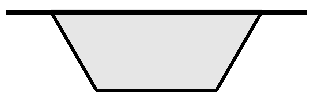
\includegraphics{fenceA.pdf}
\end{center}
\end{efig}


\soln 
 This is a very geometric problem (fenced off from pun opportunities),
and as such we should start by drawing a sketch and introducing some 
variable names.
\begin{efig}
\begin{center}
   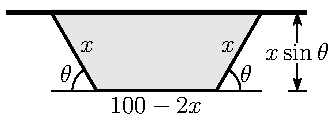
\includegraphics{fence.pdf}\quad 
   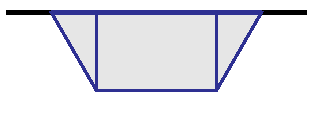
\includegraphics{fenceB.pdf}
%   \raisebox{0.13in}{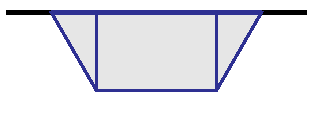
\includegraphics{fenceB.pdf}}
\end{center}
\end{efig}
The area enclosed by the fence is the area inside the blue rectangle (in the
figure on the right above) plus the area inside the two blue triangles.
\begin{align*}
A(x,\theta)
&=(100-2x)x\sin\theta+2\cdot\half\cdot x\sin\theta\cdot x\cos\theta  \\
&=(100x-2x^2)\sin\theta+ x^2\sin\theta\ \cos\theta  
\end{align*}
To maximize the area, we need to solve
\begin{align*}
0=\pdiff{A}{x}&=(100-4x)\sin\theta+2x\sin\theta\cos\theta \\
0=\pdiff{A}{\theta}
   &=(100x-2x^2)\cos\theta+x^2\big\{\cos^2\theta-\sin^2\theta\big\} 
\end{align*}
Note that both terms in the first equation contain the factor $\sin\theta$
and all terms in the second equation contain the factor $x$. If either
$\sin\theta$ or $x$ are zero the area $A(x,\theta)$ will also  be zero,
and so will certainly not be maximal. So we may divide the first equation
by $\sin\theta$ and the second equation by $x$, giving
\begin{align*}
(100-4x)+2x\cos\theta&=0 \tag{E1}\\
(100-2x)\cos\theta+x\big\{\cos^2\theta-\sin^2\theta\big\}&=0 \tag{E2}
\end{align*}
These equations might look a little scary. But there is no need to panic.
They are not as bad as they look because $\theta$ enters only through
$\cos\theta$ and $\sin^2\theta$, which we can easily write in terms
of $\cos\theta$. Furthermore we can eliminate $\cos\theta$ by observing 
that the first equation forces $\cos\theta=-\frac{100-4x}{2x}$
and hence $\sin^2\theta=1-\cos^2\theta=1-\frac{(100-4x)^2}{4x^2}$. 
Substituting these into the second equation gives
\begin{alignat*}{3}
& & -(100-2x)\frac{100-4x}{2x}+x\left[\frac{(100-4x)^2}{2x^2}-1\right]&=0 \\[0.1in]
&\implies\quad & -(100-2x)(100-4x)+(100-4x)^2-2x^2&=0 \\[0.1in]
&\implies & 6x^2-200x&=0 \\[0.1in]
&\implies & x=\frac{100}{3}
\quad\cos\theta=-\frac{-100/3}{200/3}=\frac{1}{2}\quad
\theta&=60^\circ
\end{alignat*}
and the maximum area enclosed is
\begin{equation*}
A= \Big(100\frac{100}{3}-2\frac{100^2}{3^2}\Big)\frac{\sqrt{3}}{2}
           \ +\ \frac{1}{2} \frac{100^2}{3^2}\frac{\sqrt{3}}{2}
\ =\ \frac{2500}{\sqrt{3}}
\end{equation*}
\end{eg}

Now here is a very useful (even practical!) statistical example --- finding 
the line that best fits a given collection of points.

\begin{eg}[Linear regression]\label{eg:MXMNlinReg}
An experiment yields $n$ data points $\ (x_i,y_i),\ i=1,2,\cdots,n.$ 
We wish to find the straight line $\ y=mx+b\ $ which ``best" fits the data.
\vadjust{
\begin{efig}
\begin{center}
   \includegraphics{regression.pdf}
\end{center}
\end{efig}
} 
The definition of ``best" is ``minimizes the root mean square error", 
i.e. minimizes 
\begin{equation*}
E(m,b)=\sum_{i=1}^n (mx_i+b-y_i)^2
\end{equation*}
Note that
\begin{itemize}
\item 
term number $i$ in $E(m,b)$ is the square of the difference between $y_i$,
which is the $i^{\rm th}$ measured value of $y$, and
$\Big[mx+b\Big]_{x=x_i}$, which is the approximation to $y_i$
given by the line $y=mx+b$. 
\item
All terms in the sum are positive, regardless of whether the points
$(x_i,y_i)$ are above or below the line.
\end{itemize}
Our problem is to find the $m$ and $b$ that minimizes $E(m,b)$. 
This technique for drawing a line through a bunch of
data points is called ``linear regression''. It is used 
\emph{a lot}\footnote{Proof by search engine.}
\footnote{And has been used for a long time. It was introduced
by the French mathematician Adrien-Marie Legendre, 1752--1833, in 1805, 
and by the German mathematician and physicist Carl Friedrich Gauss, 
1777--1855, in 1809.}.
Even in the real world --- and not just the real world that you find
in mathematics problems. The actual real world that involves jobs.

\soln 
 We wish to choose $m$ and $b$ so as to minimize $E(m,b)$. So we need
to determine where the partial derivatives of $E$ are zero.
\begin{alignat*}{3}
0&=\frac{\partial E}{\partial m}&&=\sum_{i=1}^n 2(mx_i+b-y_i)x_i
&&=m\Big[\smsum_{i=1}^n 2x^2_i\Big]+b\Big[\smsum_{i=1}^n 2x_i\Big]
-\Big[\smsum_{i=1}^n 2x_iy_i\Big]\\
0&=\frac{\partial E}{\partial b}&&=\sum_{i=1}^n 2(mx_i+b-y_i)
&&=m\Big[\smsum_{i=1}^n 2x_i\Big]+b\Big[\smsum_{i=1}^n 2\Big]
-\Big[\smsum_{i=1}^n 2y_i\Big]
\end{alignat*}
There are a lot of symbols here. But remember that all of the $x_i$'s and
$y_i$'s are given constants. They come from, for example, experimental data.
The only unknowns are $m$ and $b$. To emphasize this, and to save some 
writing, define the constants
\begin{equation*}
S_x=\smsum_{i=1}^n x_i\qquad
S_y=\smsum_{i=1}^n y_i\qquad
S_{x^2}=\smsum_{i=1}^n x^2_i\qquad
S_{xy}=\smsum_{i=1}^n x_iy_i
\end{equation*}
The equations which determine the critical points are (after dividing by two)
\begin{subequations}
\begin{align*}
S_{x^2}\, m+S_x\, b&=S_{xy} \tag{E1}\\
S_{x}\, m+n\, b&=S_{y}      \tag{E2}
\end{align*}
\end{subequations}
These are two linear equations on the unknowns $m$ and $b$. They may be
solved in any of the usual ways. One is to use (E2) to
solve for $b$ in terms of $m$
\begin{equation*}
b=\frac{1}{n}\big(S_y-S_xm\big)\tag{E3}
\end{equation*}
and then substitute this into (E1) to get the equation
\begin{equation*}
S_{x^2}\, m+\frac{1}{n}S_x\, \big(S_y-S_xm\big)=S_{xy}\quad\implies\quad
\big(nS_{x^2} -S_x^2\big) m = nS_{xy}-S_xS_y
\end{equation*}
for $m$. We can then solve this equation for $m$ and substitute back into
(E3) to get $b$. This gives
\begin{equation*}
m=\frac{nS_{xy}-S_xS_y}{nS_{x^2} -S_x^2}\qquad
b=-\frac{S_xS_{xy}-S_yS_{x^2}}{nS_{x^2} -S_x^2}
\end{equation*}
Another way to solve the system of equations is
\begin{alignat*}{3}
n\text{(E1)}-S_x\text{(E2)}:&\quad \Big[nS_{x^2} -S_x^2\Big]m&&=nS_{xy}-S_xS_y\\
-S_x\text{(E1)}+S_{x^2}\text{(E2)}:&\quad 
          \Big[nS_{x^2} -S_x^2\Big]b&&=-S_xS_{xy}+S_yS_{x^2}
\end{alignat*}
which gives the same solution.

So given a bunch of data points, it only takes a quick bit of arithmetic ---
no calculus required --- to apply the above formulae and so to find the 
best fitting line. Of course while you don't need any calculus to apply
the formulae, you do need calculus to understand where they came from.
The same technique can be extended to other types of curve fitting problems.
For example, polynomial regression.
\end{eg}



\subsection*{The Second Derivative Test}

Now let's start thinking about how to tell if a critical point is 
a local minimum or maximum. Remember what happens for
functions of one variable. Suppose that $x=a$ is a critical point of the
function $f(x)$. Any (sufficiently smooth) function is well approximated,
when $x$ is close to $a$, by the first few terms of its Taylor expansion
\begin{equation*}
f(x) = f(a) + f'(a)\,(x-a) + \tfrac{1}{2} f''(a)\,(x-a)^2 
         +\tfrac{1}{3!} f^{(3)}(a)\, (x-a)^3 + \cdots
\end{equation*}
As $a$ is a critical point, we know that $f'(a)=0$ and 
\begin{equation*}
f(x) = f(a) + \tfrac{1}{2} f''(a)\,(x-a)^2 
         +\tfrac{1}{3!} f^{(3)}(a)\, (x-a)^3 + \cdots
\end{equation*}
If $f''(a)\ne 0$, $f(x)$ is going to look a lot like 
$f(a) + \tfrac{1}{2} f''(a)\,(x-a)^2 $ when $x$ is really close to
$a$. In particular
\begin{itemize}
\item 
if $f''(a)>0$, then we will have $f(x)>f(a)$ when $x$
is close to (but not equal to) $a$, so that $a$ will be a local minimum
and
\item 
if $f''(a)<0$, then we will have $f(x)<f(a)$ when $x$
is close to (but not equal to) $a$, so that $a$ will be a local maximum,
but
\item 
if $f''(a)=0$, then we cannot draw any conclusions without more work.
\end{itemize}
A similar, but messier, analysis is possible for functions of
two variables. Here are some simple quadratic examples that provide 
a warmup for that messier analysis.

\begin{eg}[$f(x,y)= x^2+3xy+3y^2-6x-3y-6$]\label{eg maxminB}
Consider $f(x,y)= x^2+3xy+3y^2-6x-3y-6$. The gradient of $f$ is
\begin{equation*}
\vnabla f(x,y) = \big(2x+3y-6\big)\,\hi +\big(3x+6y-3\big)\,\hj
\end{equation*}
So $(x,y)$ is a critical point of $f$ if and only if
\begin{align*}
2x+3y&=6\tag{E1}\\
3x+6y&=3\tag{E2}
\end{align*}
Multiplying the first equation by 2 and subtracting the second equation
gives
\begin{equation*}
x=9\tag{2(E1)\ -\ (E2)}
\end{equation*}
Then substituting $x=9$ back into the first equation gives
\begin{equation*}
2\times 9+3y=6\implies
y=-4
\end{equation*}
So $f(x,y)$ has precisely one critical point, namely $(9\,,\,-4)$.

Now let's try to determine if $f(x,y)$ has a local minimum, or a local maximum,
or neither, at $(9,-4)$. A good way to determine the behaviour of $f(x,y)$
for $(x,y)$ near $(9,-4)$ is to make the change of variables\footnote{This
is equivalent to translating the graph so that the critical point 
lies at $(0,0)$.}
\begin{equation*}
x=9+\De x\qquad
y=-4+\De y
\end{equation*}
and study the behaviour of $f$ for $\De x$ and $\De y$ near zero.
\begin{align*}
f\big(9+\De x\,,\,-4+\De y\big)
&=(9+\De x)^2+3(9+\De x)(-4+\De y)+3(-4+\De y)^2\\
&\hskip1in-6(9+\De x)-3(-4+\De y)-6 \\
&= (\De x)^2 +3\De x\,\De y+3(\De y)^2 - 27
\end{align*}
And a good way to study the sign of quadratic expressions like
$(\De x)^2 +3\De x\,\De y+3(\De y)^2$ is to complete the square.
So far you have probably just completed the square for quadratic expressions 
that involve only a single variable. For example
\begin{equation*}
x^2 +3x +3 = \left(x+\frac{3}{2}\right)^2 - \frac{9}{4} +3
\end{equation*}
When there are two variables around, like $\De x$ and $\De y$,
you can just pretend that one of them is a constant and complete
the square as before. For example, if you pretend that $\De y$
is a constant,
\begin{align*}
(\De x)^2 +3\De x\,\De y+3(\De y)^2
&=\left(\De x +\frac{3}{2}\De y\right)^2  
           + \left(3-\frac{9}{4}\right)(\De y)^2\\
&=\left(\De x +\frac{3}{2}\De y\right)^2  + \frac{3}{4}(\De y)^2
\end{align*}
To this point, we have expressed
\begin{equation*}
f\big(9+\De x\,,\,-4+\De y\big)
  = \left(\De x +\frac{3}{2}\De y\right)^2  + \frac{3}{4}(\De y)^2 -27
\end{equation*}
As the smallest values of $\left(\De x +\frac{3}{2}\De y\right)^2$ 
and $\frac{3}{4}(\De y)^2$ are both zero, we have that
\begin{equation*}
f(x,y)=f\big(9+\De x\,,\,-4+\De y\big)\ge -27 =f(9,-4)
\end{equation*}
for all $(x,y)$ so that $(9,-4)$ is both a local minimum and a global minimum
for $f$. 

\end{eg}

You have already encountered single variable functions
that have a critical point which is neither a local max nor a local min. 
See Example \eref{CLP100}{eg:localMinMaxB} in the CLP-1 text.
Here are a couple of examples which show that this can also
happen for functions of two variables.
We'll start with the simplest possible such example.

\smallskip
\begin{eg}[$f(x,y)=x^2-y^2$]\label{eg maxminA}
The first partial derivatives of $f(x,y)=x^2-y^2$ are
$f_x(x,y)=2x$ and $f_y(x,y)=-2y$. So the only critical point of this function
is $(0,0)$. Is this a local minimum or maximum? Well let's start with $(x,y)$
at $(0,0)$ and then move $(x,y)$ away from $(0,0)$ and see if $f(x,y)$
gets bigger or smaller. At the origin $f(0,0)=0$. Of course we can move
$(x,y)$ away from $(0,0)$ in many different directions.
\begin{itemize}
\item
First consider moving $(x,y)$ along the $x$-axis. Then $(x,y)=(x,0)$ 
and  $f(x,y)=f(x,0)=x^2$.   So when we start with $x=0$ and then increase
$x$, the value of the function $f$ increases --- which means that $(0,0)$
cannot be a local maximum for $f$.
\item 
Next let's move $(x,y)$ away from $(0,0)$ along the $y$-axis. 
Then $(x,y)=(0,y)$ and  $f(x,y)=f(0,y)=-y^2$.   
So when we start with $y=0$ and then increase $y$, the value of the 
function $f$ decreases --- which means that  $(0,0)$ cannot be a local 
minimum for $f$.
\end{itemize}
So moving away from $(0,0)$ in one direction causes the value of $f$ to increase, while moving away from $(0,0)$ in a second direction causes 
the value of $f$ to decrease. Consequently
$(0,0)$ is neither a local minimum or maximum for $f$. It is called
a saddle point, because the graph of $f$ looks like a saddle. (The full
definition of ``saddle point'' is given immediately after this example.)
Here are some figures showing the graph of $f$.
\begin{efig}
\begin{center}
  \includegraphics[scale=3]{hyperbolic_paraboloid}\qquad
  \includegraphics{hypPara}
\end{center}
\end{efig}
The figure below show some level curves of $f$. Observe from the level 
curves that
\begin{itemize}
\item
$f$ increases as you leave $(0,0)$ walking along the $x$ axis
\item
$f$ decreases as you leave $(0,0)$ walking along the $y$ axis
\end{itemize}
\goodbreak
\begin{efig}
\begin{center}
  \includegraphics[scale=0.95]{hypParaLevel}
\end{center}
\end{efig}

\end{eg}

Approximately speaking, if a critical point $(a,b)$ is neither a local 
minimum nor a local maximum, then it is a saddle point. For $(a,b)$ to not
be a local minimum, $f$ has to take values bigger than $f(a,b)$ at some
points nearby $(a,b)$. For $(a,b)$ to not be a local maximum, $f$ has to take values smaller than $f(a,b)$ at some points nearby $(a,b)$.  Writing this
more mathematically we get the following definition.


\begin{defn}\label{def saddle point}
The critical point $(a,b)$ is called a saddle point for the function 
$f(x,y)$ if, for each $r>0$, 
\begin{itemize}
\item 
there is at least one point $(x,y)$, within a distance $r$ of $(a,b)$,
for which $f(x,y)>f(a,b)$ and
\item
there is at least one point $(x,y)$, within a distance $r$ of $(a,b)$,
for which $f(x,y)<f(a,b)$.
\end{itemize}
\end{defn}

Here is another example of a saddle point. This time we have to work
a bit to see it.

\begin{eg}[$f(x,y)= x^2-2xy-y^2+4y-2$]\label{eg maxminC}
Consider $f(x,y)= x^2-2xy-y^2+4y-2$. The gradient of $f$ is
\begin{equation*}
\vnabla f(x,y) = \big(2x-2y\big)\,\hi +\big(-2x-2y+4\big)\,\hj
\end{equation*}
So $(x,y)$ is a critical point of $f$ if and only if
\begin{align*}
2x-2y&=0 \\
-2x-2y&=-4
\end{align*}
The first equation gives that $x=y$.
Substituting $y=x$ into the second equation gives
\begin{equation*}
-2y-2y=-4\implies
x=y=1
\end{equation*}
So $f(x,y)$ has precisely one critical point, namely $(1,1)$.

To determine if $f(x,y)$ has a local minimum, or a local maximum,
or neither, at $(1,1)$, we proceed as in Example \ref{eg maxminB}.
We make the change of variables
\begin{equation*}
x=1+\De x\qquad
y=1+\De y
\end{equation*} 
to give
\begin{align*}
f\big(1+\De x\,,\,1+\De y\big)
&=(1+\De x)^2-2(1+\De x)(1+\De y)-(1+\De y)^2 + 4(1+\De y)-2 \\
&= (\De x)^2 -2\De x\,\De y-(\De y)^2 
\end{align*}
Completing the square,
\begin{equation*}
f\big(1+\De x\,,\,1+\De y\big)
=(\De x)^2 -2\De x\,\De y-(\De y)^2
=\left(\De x - \De y\right)^2  -2 (\De y)^2
\end{equation*}
Notice that $f$ has now been written as the difference of two squares, 
much like the $f$ in the saddle point Example \ref{eg maxminA}.
\begin{itemize}
\item
If $\De x$ and $\De y$ are such that the first square 
$\left(\De x - \De y\right)^2$ is nonzero, but the second square  $(\De y)^2$
is zero, then 
$f\big(1+\De x\,,\,1+\De y\big)=\left(\De x - \De y\right)^2  > 0 = f(1,1)$.
That is, whenever $\De y=0$ and $\De x\ne \De y$, then
$f\big(1+\De x\,,\,1+\De y\big)=\left(\De x - \De y\right)^2  > 0 = f(1,1)$. 
\item
On the other hand, if $\De x$ and $\De y$ are such that the first square 
$\left(\De x - \De y\right)^2$ is zero but the second square  $(\De y)^2$
is nonzero, then 
$f\big(1+\De x\,,\,1+\De y\big)=- 2(\De y)^2   < 0 = f(1,1)$.
That is, whenever $\De x=\De y\ne 0$,  then
$f\big(1+\De x\,,\,1+\De y\big) =- 2(\De y)^2 < 0 = f(1,1)$.
\end{itemize}
\begin{efig}
\begin{center}
   \includegraphics{saddle.pdf}
\end{center}
\end{efig}
So 
\begin{itemize}
\item
$f(x,y)>f(1,1)$ at all points on the blue line in the figure above, and
\item 
$f(x,y)<f(1,1)$ at all point on the red line.
\end{itemize}
We conclude that $(1,1)$ is the only critical point for $f(x,y)$,
and furthermore that it is a saddle point.

\end{eg}

The above three examples show that we can find all critical points
of quadratic functions of two variables. We can also classify 
each critical point as either a minimum, a maximum or a
saddle point. 

Of course not every function is quadratic. But by using the 
quadratic approximation \eqref{eqn quadratic approx}
we can apply the same ideas much more generally.
Suppose that $(a,b)$ is a critical point of some function $f(x,y)$. 
For $\De x$ and $\De y$ small, the
quadratic approximation \eqref{eqn quadratic approx} gives
\begin{equation*}
\begin{split}
f\big(a + \De x\,,\,b+\De y\big)
&\approx f\big(a\,,\,b\big) 
       + f_x\big(a\,,\,b\big)\,\De x
       + f_y\big(a\,,\,b\big)\,\De y \\
&\hskip0.5in +\frac{1}{2}\left\{
        f_{xx}\big(a,b\big)\,\De x^2
       +2f_{xy}\big(a,b\big) \,\De x\De y 
       + f_{yy}\big(a,b\big)\,\De y^2 \right\}\\
&= f\big(a\,,\,b\big) 
        +\frac{1}{2}\left\{
        f_{xx}\big(a,b\big)\,\De x^2
       +2f_{xy}\big(a,b\big) \,\De x\De y 
       + f_{yy}\big(a,b\big)\,\De y^2 \right\}
\end{split}\tag{$*$}
\end{equation*}
since $(a,b)$ is a critical point so that $f_x(a,b)=f_y(a,b)=0$.
Then using the technique of Examples \ref{eg maxminB} and \ref{eg maxminC}, 
we get\footnote{There are analogous results in higher dimensions that are accessible to people who have learned some linear algebra. They
are derived by diagonalizing the matrix of second derivatives, which is 
called the Hessian matrix.
} 
(details below)


\begin{theorem}[Second Derivative Test]\label{thm second deriv test}
Let $r>0$ and assume that all second order derivatives of the function 
$f(x,y)$ are continuous at all points $(x,y)$ that are within a distance
$r$ of $(a,b)$. Assume that $f_x(a,b)=f_y(a,b)=0$. 
Define
\begin{equation*}
D(x,y) = f_{xx}(x,y)\,f_{yy}(x,y) - f_{xy}(x,y)^2
\end{equation*}
It is called the discriminant of $f$. Then
\begin{itemize}
\item 
if $D(a,b)>0$ and $f_{xx}(a,b)>0$, then $f(x,y)$ has a local minimum 
at $(a,b)$, 
\item 
if $D(a,b)>0$ and $f_{xx}(a,b)<0$, then $f(x,y)$ has a local maximum 
at $(a,b)$, 
\item 
if $D(a,b)<0$, then $f(x,y)$ has a saddle point at $(a,b)$, but
\item 
if $D(a,b)=0$, then we cannot  draw any conclusions without more work.
\end{itemize}
\end{theorem}

\begin{proof}[``Proof'']
We are putting quotation marks around the word ``Proof'',
because we are not going to justify the fact that it suffices
to analyse the quadratic approximation in equation~$(*)$. 
Let's temporarily suppress the arguments $(a,b)$.
If $f_{xx}(a,b)\ne 0$, then by completing the square we can write
\begin{align*}
f_{xx}\,\De x^2
       +2f_{xy}\,\De x\De y 
       + f_{yy}\,\De y^2 
&=f_{xx}\left(\De x
       +\frac{f_{xy}}{f_{xx}}\De y\right)^2 
       +\left(f_{yy}-\frac{f_{xy}^2}{f_{xx}}\right)\,\De y^2 \\
&=\frac{1}{f_{xx}}\left\{\big(f_{xx}\,\De x+f_{xy}\,\De y\big)^2
                         +\big(f_{xx}f_{yy}-f_{xy}^2\big)\,\De y^2\right\}
\end{align*}
Similarly, if $f_{yy}(a,b)\ne 0$,
\begin{align*}
f_{xx}\,\De x^2
       +2f_{xy}\,\De x\De y 
       + f_{yy}\,\De y^2 
&=\frac{1}{f_{yy}}\left\{\big(f_{xy}\,\De x+f_{yy}\,\De y\big)^2
                         +\big(f_{xx}f_{yy}-f_{xy}^2\big)\,\De x^2\right\}
\end{align*}
Note that this algebra breaks down if $f_{xx}(a,b)=f_{yy}(a,b)=0$.
We'll deal with that case shortly. More importantly, note that
\begin{itemize}
\item
if $\big(f_{xx}f_{yy}-f_{xy}^2\big)>0$ then both $f_{xx}$ and $f_{yy}$ must
be nonzero and of the same sign and furthermore, whenever $\De x$ 
or $\De y$ are nonzero,
\begin{align*}
\left\{\big(f_{xx}\,\De x+f_{xy}\,\De y\big)^2
                         +\big(f_{xx}f_{yy}-f_{xy}^2\big)\,\De y^2\right\}
&>0\quad\text{and} \\
\left\{\big(f_{xy}\,\De x+f_{yy}\,\De y\big)^2
                         +\big(f_{xx}f_{yy}-f_{xy}^2\big)\,\De x^2\right\}
&>0
\end{align*}
so that, recalling $(*)$,
\begin{itemize}
\item
if $f_{xx}(a,b)>0$, then $(a,b)$ is a local minimum and
\item
if $f_{xx}(a,b)<0$, then $(a,b)$ is a local maximum.
\end{itemize}

\item
If $\big(f_{xx}f_{yy}-f_{xy}^2\big)<0$ and $f_{xx}$ is nonzero then
\begin{equation*}
\left\{\big(f_{xx}\,\De x+f_{xy}\,\De y\big)^2
                         +\big(f_{xx}f_{yy}-f_{xy}^2\big)\,\De y^2\right\}
\end{equation*}
is strictly positive whenever $\De x\ne 0$, $\De y= 0$ and is
strictly negative whenever $f_{xx}\,\De x+f_{xy}\,\De y=0$, $\De y\ne 0$, 
so that $(a,b)$ is a saddle point. Similarly, $(a,b)$ is also a saddle point
if $\big(f_{xx}f_{yy}-f_{xy}^2\big)<0$ and $f_{yy}$ is nonzero.

\item
Finally, if $f_{xy}\ne 0$ and $f_{xx}=f_{yy}=0$, then
\begin{equation*}
f_{xx}\,\De x^2
       +2f_{xy}\,\De x\,\De y 
       + f_{yy}\,\De y^2 
=2f_{xy}\,\De x\,\De y 
\end{equation*}
is strictly positive for one sign of $\De x\,\De y$ and is strictly
negative for the other sign of $\De x\,\De y$. So 
$(a,b)$ is again a saddle point.
\end{itemize}
\end{proof}

You might wonder why, in the local maximum/local minimum cases
of Theorem \ref{thm second deriv test}, $f_{xx}(a,b)$ appears rather 
than $f_{yy}(a,b)$. The answer
is only that $x$ is before $y$ in the alphabet\footnote{The shackles of convention are not limited to mathematics. Election ballots often have the candidates listed in alphabetic order.}. You can use $f_{yy}(a,b)$
just as well as $f_{xx}(a,b)$. The reason is that if 
$D(a,b)>0$ (as in the first two bullets of the theorem),
then because $D(a,b) = f_{xx}(a,b)\,f_{yy}(a,b) - f_{xy}(a,b)^2>0$,
we necessarily have $f_{xx}(a,b)\,f_{yy}(a,b)>0$ so that 
$f_{xx}(a,b)$ and $f_{yy}(a,b)$ must have the same sign --- either both
are positive or both are negative.

You might also wonder why we cannot draw any conclusions when $D(a,b)=0$
and what happens then. The second derivative test for functions
 of two variables was derived in precisely the same way as the second derivative
test for functions of one variable is derived --- you approximate the function
by a polynomial that is of degree two in $(x-a)$, $(y-b)$ and then
you analyze the behaviour of the quadratic polynomial near $(a,b)$.
For this to work, the contributions to $f(x,y)$ from terms that 
are of degree two in  $(x-a)$, $(y-b)$ had better be bigger than  
the contributions to $f(x,y)$ from terms that are of degree three
and higher in  $(x-a)$, $(y-b)$ when $(x-a)$, $(y-b)$ are really small. 
If this is not the case, for example when the terms in $f(x,y)$ that are 
of degree two in  $(x-a)$, $(y-b)$ all have coefficients that are exactly 
zero, the analysis will certainly break down. That's exactly what happens 
when $D(a,b)=0$. Here are some examples. The functions
\begin{equation*}
f_1(x,y)=x^4+y^4\qquad
f_2(x,y)=-x^4-y^4\qquad
f_3(x,y)=x^3+y^3\qquad
f_4(x,y)=x^4-y^4
\end{equation*}
all have $(0,0)$ as the only critical point and all have $D(0,0)=0$. 
The first, $f_1$ has its minimum there. The second, $f_2$, has 
its maximum there. The third and fourth have a saddle point there.

Here are sketches of some level curves for each of these four functions
(with all renamed to simply $f$).

\begin{efig}
\begin{center}
   \includegraphics{f1Level.pdf}\qquad
   \includegraphics{f2Level.pdf}\qquad
\end{center}
\end{efig}


\begin{efig}
\begin{center}
   \includegraphics{f3Level.pdf}\qquad
   \includegraphics{f4Level.pdf}\qquad
\end{center}
\end{efig}


\goodbreak
\medskip
\begin{eg}[$f(x,y)=2x^3 - 6xy + y^2 +4y $]\label{eg:MXMNlocalBb}
Find and classify all critical points of $f(x,y)=2x^3 - 6xy + y^2 +4y $.

\soln 
Thinking a little way ahead, to find the critical points we will need the
gradient and to apply the second derivative test of 
Theorem \ref{thm second deriv test} we will need all second order partial derivatives. So we need all partial derivatives of order up to two.
Here they are.
\begin{alignat*}{3}
f&=2x^3 - 6xy + y^2 +4y \hidewidth\\
f_x&=6x^2-6y   & f_{xx}&=12x \qquad & f_{xy}&= -6\\
f_y&=-6x+2y+4 \qquad & f_{yy}&=2\qquad & f_{yx}&= -6
\end{alignat*}
(Of course, $f_{xy}$ and $f_{yx}$ have to be the same. It is still
useful to compute both, as a way to catch some mechanical errors.)

We have already found, in Example \ref{eg:MXMNlocalB}, 
that the critical points are $(1,1),\ (2,4)$. The classification is
\begin{center}
\renewcommand{\arraystretch}{1.3}
     \begin{tabular}{|c|c|c|c|}
     \hline
    $\Atop{\text{critical}}{\text{point}}$  & $f_{xx}f_{yy}-f_{xy}^2$ & 
                                                          $f_{xx}$ & type \\    
    \hline
     $(1,1)$  & $12\times 2-(-6)^2<0$ &    & saddle point  \\ \hline
     $(2,4)$  & $24\times 2-(-6)^2>0$ & 24 & local min \\  \hline
     \end{tabular}
\renewcommand{\arraystretch}{1.0}
\end{center}
We were able to leave the $f_{xx}$ entry in the top row blank, because
\begin{itemize}\itemsep1pt \parskip0pt \parsep0pt
\item
we knew that $f_{xx}(1,1) f_{yy}(1,1)-f_{xy}^2(1,1)<0$, and 
\item
we knew, from Theorem \ref{thm second deriv test}, 
that $f_{xx}(1,1) f_{yy}(1,1)-f_{xy}^2(1,1)<0$, by itself,
was enough to ensure that $(1,1)$ was a saddle point.
\end{itemize}
Here is a sketch of some level curves of our $f(x,y)$.
\vadjust{
\begin{efig}
\begin{center}
   \includegraphics{fALevel.pdf}
\end{center}
\end{efig}
} 
They are not needed to answer this question, but can give you
some idea as to what the graph of $f$ looks like.
\end{eg}


\begin{eg}[$f(x,y) = xy(5x+y-15)$]\label{eg:MXMNlocalCc}
Find and classify all critical points of $f(x,y)=xy(5x+y-15)$.

\soln 
We have already computed the first order partial derivatives
\begin{equation*}
f_x(x,y)= y(10x+y-15)\qquad\qquad
f_y(x,y)= x(5x+2y-15)
\end{equation*} 
of $f(x,y)$ in Example \ref{eg:MXMNlocalC}.
Again, to classify the critical points we need the second order 
partial derivatives. They  are
\begin{alignat*}{3}
f_{xx}(x,y)&= 10y \\
f_{yy}(x,y)&= 2x \\
f_{xy}(x,y)&= (1)(10x+y-15)+y(1) &= 10x+2y-15 
 \\ f_{yx}(x,y)&= (1)(5x+2y-15)+x(5) &= 10x+2y-15 
\end{alignat*}
(Once again, we have computed both $f_{xy}$ and $f_{yx}$ to guard against
mechanical errors.)
We have already found, in Example \ref{eg:MXMNlocalC}, 
that the critical points are $(0,0),\ (0,15),\ (3,0)$ and $(1,5)$. 
The classification is
\begin{center}
\renewcommand{\arraystretch}{1.3}
     \begin{tabular}{|c|c|c|c|}
     \hline
    $\Atop{\text{critical}}{\text{point}}$  & $f_{xx}f_{yy}-f_{xy}^2$ & 
                                                          $f_{xx}$ & type \\    
    \hline
   $(0,0)$  & $0\times0-(-15)^2<0$ & & saddle point \\ \hline
   $(0,15)$ & $150\times0-15^2<0$ & & saddle point \\ \hline
   $(3,0)$  & $0\times 6-15^2<0$  & & saddle point \\ \hline
   $(1,5)$  & $50\times 2-5^2>0$ & 50 & local min \\ \hline
     \end{tabular}
\renewcommand{\arraystretch}{1.0}
\end{center}

Here is a sketch of some level curves of our $f(x,y)$. $f$ is negative
in the shaded regions and $f$ is positive in the unshaded regions.
\vadjust{
\begin{efig}
\begin{center}
   \includegraphics{fBLevel.pdf}
\end{center}
\end{efig}
}
Again this is not needed to answer this question, but can give you
some idea as to what the graph of $f$ looks like.

\end{eg}
\goodbreak

\begin{eg}\label{eg max min A}
Find and classify all of the critical points of $f(x,y)=x^3+xy^2-3x^2-4y^2+4$.

\medskip
\noindent\textit{Solution}.
We know the drill now. We start by computing all of the partial 
derivatives of $f$ up to order 2.
\begin{align*}
f&=x^3+xy^2-3x^2-4y^2+4 \hidewidth\\
f_x&=3x^2+y^2-6x & f_{xx}&=6x-6 & f_{xy}&= 2y\\
f_y&=2xy-8y & f_{yy}&=2x-8  & f_{yx}&= 2y
\end{align*}
The critical points are then the solutions of $f_x=0$, $f_y=0$. That is
\begin{align*}
f_x&=3x^2+y^2-6x=0 \tag{E1}\\
f_y&=2y(x-4)=0 \tag{E2}
\end{align*}
The second equation, $2y(x-4)=0 $, is satisfied if and only if at least 
one of the two equations $y=0$ and $x=4$ is satisfied.
\begin{itemize}
\item
When $y=0$, equation (E1) forces $x$ to obey 
\begin{equation*}
0=3x^2+0^2-6x=3x(x-2)
\end{equation*}
so that $x=0$ or $x=2$.
\item
When $x=4$, equation (E1) forces $y$ to obey 
\begin{equation*}
0=3\times 4^2+y^2-6\times 4=24+y^2
\end{equation*} 
which is impossible.
\end{itemize}
So, there are two critical points: $(0,0),\ (2,0)$.
Here is a table that classifies the critical points.

\begin{center}
\renewcommand{\arraystretch}{1.5}
\begin{tabular}{ | c | c | c | c |}
\hline
$\Atop{\rm critical}{\rm point}$ & $f_{xx}f_{yy}-f_{xy}^2$ & $f_{xx}$ & type \\
\hline
$(0,0)$ & $(-6)\times (-8)-0^2>0$ & $-6<0$ & local max \\
\hline
$(2,0)$ & $6\times(-4)-0^2<0$ & & saddle point \\
\hline
\end{tabular}
\renewcommand{\arraystretch}{1.0}
\end{center}

\end{eg}



\begin{eg}\label{eg max min B}
A manufacturer wishes to make an open rectangular box of given volume $V$
using the least possible material. Find the design specifications.

\medskip
\noindent\textit{Solution}.
Denote by $x$, $y$ and $z$, the length, width and height, respectively,
of the box.
\begin{efig}
\begin{center}
   \includegraphics{box.pdf}
\end{center}
\end{efig}
The box has two sides of area $xz$, two sides of area $yz$ and a bottom
of area $xy$. So the total surface area of material used is
\begin{equation*}
S = 2xz + 2yz + xy
\end{equation*}
However the three dimensions $x$, $y$ and $z$ are not independent. The
requirement that the box have volume $V$ imposes the constraint
\begin{equation*}
xyz = V
\end{equation*}
We can use this constraint to eliminate one variable. Since $z$
is at the end of the alphabet (poor $z$), we eliminate $z$
by substituting $z=\frac{V}{xy}$. So we have find the values of $x$ and 
$y$ that minimize the function 
\begin{equation*}
S(x,y) = \frac{2V}{y} + \frac{2V}{x} + xy
\end{equation*}
Let's start by finding the critical points of $S$. Since
\begin{align*}
S_x(x,y) &= -\frac{2V}{x^2} + y \\[0.1in]
S_y(x,y) &= -\frac{2V}{y^2} + x
\end{align*}
$(x,y)$ is a critical point if and only if
\begin{align*}
x^2y&=2V \tag{E1} \\
xy^2&=2V \tag{E2}
\end{align*}
Solving (E1) for $y$ gives $y=\frac{2V}{x^2}$. Substituting this into
(E2) gives
\begin{equation*}
x\frac{4V^2}{x^4}=2V \implies
x^3 = 2V \implies  x = \root{3}\of{2V}\quad\text{and}\quad
                   y = \frac{2V}{(2V)^{2/3}} = \root{3}\of{2V}
\end{equation*}
As there is only one critical point, we would expect it to give the
minimum\footnote{Indeed one can use the facts that $0<x<\infty$, that
$0<y<\infty$, and that $S\rightarrow\infty$ as $x\rightarrow 0$ and
as $y\rightarrow 0$ and as $x\rightarrow \infty$ and as 
$y\rightarrow\infty$ to prove that the single critical point gives the
global minimum.}. But let's use the second derivative test to verify that
at least the critical point is a local minimum. The various second partial derivatives are
\begin{align*}
S_{xx}(x,y)&=\frac{4V}{x^3} &
    S_{xx}\big(\root{3}\of{2V}\,,\,\root{3}\of{2V}\big)&=2 \\
S_{xy}(x,y)&=1&
    S_{xy}\big(\root{3}\of{2V}\,,\,\root{3}\of{2V}\big)&=1 \\
S_{yy}(x,y)&=\frac{4V}{y^3} &
    S_{yy}\big(\root{3}\of{2V}\,,\,\root{3}\of{2V}\big)&=2 
\end{align*}
So
\begin{align*}
S_{xx}\big(\root{3}\of{2V}\,,\,\root{3}\of{2V}\big)\ 
S_{yy}\big(\root{3}\of{2V}\,,\,\root{3}\of{2V}\big)
-S_{xy}\big(\root{3}\of{2V}\,,\,\root{3}\of{2V}\big)^2
=3>0\qquad
S_{xx}\big(\root{3}\of{2V}\,,\,\root{3}\of{2V}\big)=2>0
\end{align*}
and, by Theorem \ref{thm second deriv test}.b,
$\big(\root{3}\of{2V}\,,\,\root{3}\of{2V}\big)$ is a local 
minimum and the desired dimensions are
\begin{equation*}
x=y=\root{3}\of{2V}\qquad
z=\root{3}\of{\frac{V}{4}}
\end{equation*}
Note that our solution has $x=y$. That's a good thing --- the
function $S(x,y)$ is symmetric in $x$ and $y$. Because the box has
no top, the symmetry does not extend to $z$.
\end{eg} 



\subsection{Absolute Minima and Maxima}\label{sec global}


Of course a local maximum or minimum of a function need not be the 
absolute maximum of minimum. We'll now consider how to find the 
absolute maximum and minimum.
Let's start by reviewing how one finds the absolute maximum and minimum 
of a function of one variable on an interval. 

For concreteness, let's suppose that we
want to find the extremal\footnote{Recall that ``extremal value''
means ``either maximum value or minimum value''.} values of a function 
$f(x)$ on the interval $0\le x\le 1$. If an extremal value is attained 
at some $x=a$ which is in the interior of the interval, i.e. if $0<a<1$, 
then $a$ is also a local maximum or minimum and so has to be a critical 
point of $f$. But if 
an extremal value is attained at a boundary point $a$ of the interval, 
i.e. if $a=0$ or $a=1$, then $a$ need not be a critical point of $f$. 
This happens, for example, when $f(x)=x$. The largest value of $f(x)$ on 
the interval $0\le x\le 1$ is $1$ and is attained at $x=1$, but $f'(x)=1$ 
is never zero, so that $f$ has no critical points.
\begin{efig}
\begin{center}
  \includegraphics{absMaxMin}
\end{center}
\end{efig}
So to find the maximum and minimum of the function $f(x)$ on the interval
$[0,1]$, you
\begin{enumerate}
\item build up a list of all candidate points $0\le a\le 1$ at which 
the maximum or minimum could be attained, by finding all $a$'s for which
either
   \begin{enumerate}
   \item $0<a<1$ and $f'(a)=0$ or
   \item $0<a<1$ and $f'(a)$ does not exist\footnote{Recall that if $f'(a)$ does not exist, then $a$ is called a singular point of $f$.} or
   \item $a$ is a boundary point, i.e. $a=0$ or $a=1$,
   \end{enumerate}
\item and then you evaluate $f(a)$ at each $a$ on the list of candidates.
   The biggest of these candidate values of $f(a)$ is the absolute maximum and the
   smallest of these candidate values is the absolute minimum.
\end{enumerate}

The procedure for finding the maximum and minimum of a function of two
variables, $f(x,y)$ in a set like, for example, the unit disk $x^2+y^2\le 1$, 
is similar.  You again
\begin{enumerate}
\item build up a list of all candidate points $(a,b)$ in the set at which 
the maximum or minimum could be attained, by finding all $(a,b)$'s for which
either\footnote{This is probably a good time to review the statement of
Theorem \ref{thm stationary point}.}
   \begin{enumerate}
   \item $(a,b)$ is in the interior of the set (for our example, $a^2+b^2<1$)
    and $f_x(a,b)=f_y(a,b)=0$ or
   \item $(a,b)$ is in the interior of the set and  $f_x(a,b)$ or $f_y(a,b)$
        does not exist or
   \item $(a,b)$ is a boundary\footnote{It should intuitively obvious 
       from a sketch that the boundary of the disk $x^2+y^2\le 1$ is 
       the circle $x^2+y^2=1$.
       But if you really need a formal definition, here it is. A point
       $(a,b)$ is on the boundary of a set $S$ if there is a sequence of
       points in $S$ that converges to $(a,b)$ and there is also a sequence
       of points in the  complement of $S$ that converges to $(a,b)$.} 
     point, (for our example, $a^2+b^2=1$), and 
        could give the maximum or minimum on the boundary --- 
        more about this shortly ---
   \end{enumerate}
\item and then you evaluate $f(a,b)$ at each $(a,b)$ on the list of candidates.
   The biggest of these candidate values of $f(a,b)$ is the absolute maximum 
   and the smallest of these candidate values is the absolute minimum.
\end{enumerate}
The boundary of a set, like $x^2+y^2\le 1$, in $\bbbr^2$ is a curve,
like $x^2+y^2=1$. This curve is a one dimensional set, meaning that it
is like a deformed $x$-axis. We can find the maximum and minimum of $f(x,y)$
on this curve by converting $f(x,y)$ into a function of one variable (on the
curve) and using the standard function of one variable techniques. This is
best explained by some examples.

\begin{eg}\label{eg:MXMNabsA}
Find the maximum and minimum of $T(x,y)=(x+y)e^{-x^2-y^2}$
on the region defined by $x^2+y^2\le 1$ (i.e. on the unit disk).

\soln 
Let's follow our checklist. First critical points, then points where
the partial derivatives don't exist, and finally the boundary.

\noindent\emph{Interior Critical Points:}\ \ 
If $T$ takes its maximum or minimum value at a point in the interior, 
$x^2+y^2<1$, then that point must be either a critical point of $T$ or a singular point of $T$.
To find the critical points we compute the first order derivatives.
\begin{equation*}
T_x(x,y)=(1-2x^2-2xy)e^{-x^2-y^2}\qquad
T_y(x,y)=(1-2xy-2y^2)e^{-x^2-y^2}
\end{equation*}
Because the exponential $e^{-x^2-y^2}$ is never zero, 
the critical points are the solutions of
\begin{alignat*}{3}
T_x&=0 &\quad&\iff\quad & 2x(x+y)&=1 \\
T_y&=0 & &\iff & 2y(x+y)&=1  
\end{alignat*}
\begin{itemize}
\item
As both $2x(x+y)$ and $2y(x+y)$ are nonzero, we may divide the 
two equations, which gives $\frac{x}{y}=1$, forcing $x=y$. 
\item
Substituting this into either
equation gives $2x(2x)=1$ so that $x=y=\pm\nicefrac{1}{2}$.
\end{itemize}
So the only critical points are $(\nicefrac{1}{2},\nicefrac{1}{2})$ 
and $(-\nicefrac{1}{2},-\nicefrac{1}{2})$. Both are in $x^2+y^2<1$.

\smallskip
\noindent\emph{Singular points:}\ \  In this problem, there are no singular 
points.

\smallskip
\noindent\emph{Boundary:}\ \ 
Points on the boundary satisfy $x^2+y^2=1$. That is they lie on a circle. 
We may use the figure below to express $x=\cos t$ and $y=\sin t$, in terms
of the angle $t$. This will make the formula for $T$ on the boundary quite a 
bit easier to deal with. On the boundary,
\begin{equation*}
T = (\cos t+\sin t)e^{-\cos^2 t -\sin^2 t}
=(\cos t+\sin t)e^{-1}
\end{equation*}
As all $t$'s are allowed, this function takes its max and min at zeroes of
\vadjust{
\begin{efig}
\begin{center}
  \includegraphics{optExampleAa}
\end{center}
\end{efig}
}
\begin{equation*}
\frac{dT}{dt}=\big(-\sin t+\cos t\big)e^{-1}
\end{equation*}
That is, $(\cos t+\sin t)e^{-1}$ takes its max and min 
\begin{itemize}
\item
when $\sin t=\cos t$,
\item
that is, when $x=y$ and $x^2+y^2=1$, 
\item
which forces $x^2+x^2=1$ and hence $x=y=\pm\tfrac{1}{\sqrt{2}}$. 
\end{itemize}
All together, we have the following candidates for max and min, with the
max and min indicated.
\begin{center}
\renewcommand{\arraystretch}{1.3}
     \begin{tabular}{|c|c|c|c|c|}
     \hline
       point
       &\raisebox{2pt}{$(\half,\half)$}
       &\raisebox{2pt}{$(-\half,-\half)$}
       &\raisebox{2pt}{$(\tfrac{1}{\sqrt{2}},\tfrac{1}{\sqrt{2}})$} 
       &\raisebox{2pt}{$(-\tfrac{1}{\sqrt{2}},-\tfrac{1}{\sqrt{2}})$} \\ \hline
       value of $T$
       &\raisebox{2pt}{$\tfrac{1}{\sqrt{e}}\approx0.61$}
       &\raisebox{2pt}{$-\tfrac{1}{\sqrt{e}}$}
       &$\tfrac{\sqrt{2}}{e}\approx0.52$
       &$-\tfrac{\sqrt{2}}{e}$ \\ \hline
       & max 
       & min
       & & \\ \hline
     \end{tabular}
\renewcommand{\arraystretch}{1.0}
\end{center}
The following sketch shows all of the critical points. It is a good idea
to make such a sketch so that you don't accidentally include a critical
point that is outside of the allowed region.
\begin{efig}
\begin{center}
   \includegraphics{optExampleA}
\end{center}
\end{efig}
\end{eg}
\goodbreak

In the last example, we analyzed the behaviour of $f$ on the boundary
of the region of interest by using the parametrization $x=\cos t$, $y=\sin t$
of the circle $x^2+y^2=1$. Sometimes using this parametrization is not
so clean. And worse, some curves don't have such a simple parametrization.
In the next problem we'll look at the boundary a little differently. 

\begin{eg}\label{eg:MXMNabsB}
Find the maximum and minimum values of $f(x,y)=x^3+xy^2-3x^2-4y^2+4$
on the disk $x^2+y^2\le 1$.

\soln 
Again, we first find all critical points, then find all singular points
and, finally, analyze the boundary.

\noindent\emph{Interior Critical Points:}\ \ 
If $f$ takes its maximum or minimum value at a point in the interior, 
$x^2+y^2<1$, then that point must be either a critical point of $f$ 
or a singular point of $f$.
To find the critical points\footnote{We actually found the critical points in
Example \ref{eg max min A}. But, for the convenience of the reader, we'll repeat that here.} we compute the first order derivatives.
\begin{align*}
f_x=3x^2+y^2-6x \qquad
f_y=2xy-8y 
\end{align*}
The critical points are the solutions of
\begin{align*}
f_x&=3x^2+y^2-6x=0 \tag{E1}\\
f_y&=2y(x-4)=0 \tag{E2}
\end{align*}
The second equation, $2y(x-4)=0 $, is satisfied if and only if at least 
one of the two equations $y=0$ and $x=4$ is satisfied.
\begin{itemize}
\item
When $y=0$, equation (E1) forces $x$ to obey 
\begin{equation*}
0=3x^2+0^2-6x=3x(x-2)
\end{equation*}
so that $x=0$ or $x=2$.
\item
When $x=4$, equation (E1) forces $y$ to obey 
\begin{equation*}
0=3\times 4^2+y^2-6\times 4=24+y^2
\end{equation*} 
which is impossible.
\end{itemize}
So, there are only two critical points: $(0,0),\ (2,0)$.

\smallskip
\noindent\emph{Singular points:}\ \  In this problem, there are no singular 
points.


\smallskip
\noindent\emph{Boundary:}\ \ 
On the boundary, $x^2+y^2=1$, we could again take advantage of having 
a circle and write $x=\cos t$ and $y=\sin t$. 
But, for practice, we'll use another method\footnote{Even if you
don't believe that ``you can't have too many tools'', it is pretty dangerous
to have to rely on just one tool.}. We know that $(x,y)$ satisfies 
$x^2+y^2=1$, and hence $y^2=1-x^2$. Examining the formula for $f(x,y)$,
we see that it contains only even\footnote{If it contained odd powers too,
we could consider the cases $y\ge 0$ and $y\le 0$ separately and
substitute $y=\sqrt{1-x^2}$ in the former case and $y=-\sqrt{1-x^2}$
in the latter case.} powers of $y$, so we can eliminate $y$
by substituting $y^2=1-x^2$ into the formula.
\begin{equation*}
f=x^3+x(1-x^2)-3x^2-4(1-x^2)+4=x+x^2
\end{equation*}
The max and min of $x+x^2$ for $-1\le x\le 1$ must occur either
\begin{itemize}
\item  when $x=-1$ ($\Rightarrow y=f=0$) or 
\item when $x=+1$ ($\Rightarrow y=0$, $f=2$) or
\item  when $0=\frac{d\hfill}{dx}(x+x^2)=1+2x$ ($\Rightarrow x=-\half$, 
$y=\pm\sqrt{\frac{3}{4}}$, $f=-\frac{1}{4}$). 
\end{itemize}
Here is a sketch showing all of the points that we have identified.
\begin{efig}
\begin{center}
   \includegraphics[scale=0.95]{optExampleB}
\end{center}
\end{efig}
Note that the point $(2,0)$ is outside the allowed region\footnote{We 
found $(2,0)$ as a solution to the critical point equations (E1), (E2).
That's because, in the course of solving those equations, 
we ignored the constraint that $x^2+y^2\le 1$.}.
So all together, we have the following candidates for max and min, with the
max and min indicated.
\begin{center}
\renewcommand{\arraystretch}{1.3}
     \begin{tabular}{|c|c|c|c|c|}
     \hline
       point
       &$(0,0)$
       &$(-1,0)$
       &$(1,0)$
       &$\big(-\half,\pm\tfrac{\sqrt{3}}{2}\big)$ \\ \hline
       value of $f$
       &$4$
       &$0$
       &$2$
       &$-\tfrac{1}{4}$ \\ \hline
       &max
       & 
       & 
       &min \\ \hline
     \end{tabular}
\renewcommand{\arraystretch}{1.0}
\end{center}
\end{eg}
\goodbreak

\begin{eg}\label{eg:MXMNabsC}
Find the maximum and minimum values of $f(x,y)=xy-x^3y^2$ when $(x,y)$
runs over the square $0\le x\le 1,\ 0\le y\le 1$.
\goodbreak

\soln 
As usual, let's examine the critical points, singular points and boundary
in turn.

\noindent\emph{Interior Critical Points:}\ \ 
If $f$ takes its maximum or minimum value at a point in the interior, 
$0<x<1$, $0<y<1$, then that point must be either a critical point of $f$
or a singular point of $f$.
To find the critical points we compute the first order derivatives.
\begin{equation*}
f_x(x,y)=y-3x^2y^2\qquad
f_y(x,y)=x-2x^3y
\end{equation*}
The critical points are the solutions of
\begin{alignat*}{5}
f_x&=0 & &\quad\iff\quad  &y(1-3x^2y)=0 & 
         &\quad\iff\quad & &y=0 \ \text{ or }\  3x^2y=1 \\
f_y&=0 & &\quad\iff\quad  &x(1-2x^2y)=0 & 
          &\quad\iff\quad & &x=0 \ \text{ or }\  2x^2y=1 
\end{alignat*}
\begin{itemize}
\item 
If $y=0$, we cannot have $2x^2y=1$, so we must have $x=0$.
\item
If $3x^2y=1$, we cannot have $x=0$, so we must have $2x^2y=1$. Dividing
gives $1=\tfrac{3x^2y}{2x^2y}=\tfrac{3}{2}$ which is impossible.
\end{itemize}
So the only critical point in the square is $(0,0)$. There $f=0$.

\smallskip
\noindent\emph{Singular points:}\ \  Yet again there are no singular 
points in this problem.


\smallskip
\noindent\emph{Boundary:}\ \ 
The region is a square, so its boundary consists of its four sides.
\begin{itemize}
\item 
First, we look at the part of the boundary with $x=0$. On that entire 
       side $f=0$.
\item 
Next, we look at the part of the boundary with $y=0$. On that entire side 
  $f=0$.
\item
Next, we look at the part of the boundary with $y=1$. There $f=f(x,1)=x-x^3$.
To find the maximum and minimum of $f(x,y)$ on the part of the boundary
with $y=1$, we must find the maximum and minimum of $x-x^3$ when 
 $0\le x\le 1$. 

Recall that, in general, the maximum and minimum of a 
function $h(x)$ on the interval $a\le x\le b$, must occur either at $x=a$ 
or at $x=b$ or at an $x$ for which either 
$h'(x)=0$ or $h'(x)$ does not exist. In this case,
$\tfrac{d\hfill}{dx}(x-x^3)=1-3x^2$, so the max and min of $x-x^3$ for 
$0\le x\le 1$ must occur 
\begin{itemize}\itemsep1pt \parskip0pt \parsep0pt
\item
either at $x=0$, where $f=0$, 
\item 
or at $x=\tfrac{1}{\sqrt{3}}$, where $f=\tfrac{2}{3\sqrt{3}}$, 
\item
or at $x=1$, where $f=0$.
\end{itemize}
\item
 Finally, we look at the part of the boundary with $x=1$. There $f=f(1,y)=y-y^2$.
 As $\tfrac{d\hfill}{dy}(y-y^2)=1-2y$, the only critical point of $y-y^2$
is at $y=\frac{1}{2}$. So the the max and min of $y-y^2$ for $0\le y\le 1$ 
must occur
\begin{itemize}\itemsep1pt \parskip0pt \parsep0pt
\item
 either at $y=0$, where $f=0$, 
\item 
or at $y=\half$,  where $f=\tfrac{1}{4}$, 
\item
or at $y=1$, where $f=0$.
\end{itemize}
\end{itemize}
All together, we have the following candidates for max and min, with the
max and min indicated.
\begin{center}
\renewcommand{\arraystretch}{1.3}
     \begin{tabular}{|c|c|c|c|c|c|c|c|c|}
     \hline
       point
       &$(0,0)$
%       &$(0,0\le y\le 1)$
%       &$(0\le x\le 1,0)$  
       &${\scriptstyle(0,0\le y\le 1)}$
       &${\scriptstyle(0\le x\le 1,0)}$  
       &$(1,0)$
       &$(1,\half)$
       &$(1,1)$
       &$(0,1)$
       &$(\tfrac{1}{\sqrt{3}},1)$ \\   \hline
       value of $f$
       &0
       &0
       &0
       &0
       &$\tfrac{1}{4}$
       &0
       &0
       &$\tfrac{2}{3\sqrt{3}}\approx0.385$ \\ \hline
       &min
       &min
       &min
       &min
       & 
       &min
       &min
       &max \\ \hline
     \end{tabular}
\renewcommand{\arraystretch}{1.0}
\end{center}

\begin{efig}
\begin{center}
   \includegraphics{optExampleC}
\end{center}
\end{efig}
\end{eg}
\goodbreak

\begin{eg}\label{eg:MXMNabsCC}
Find the maximum and minimum values of $f(x,y)=xy+2x+y$ when $(x,y)$
runs over the triangular region with vertices $(0,0)$, $(1,0)$ and
$(0,2)$. The triangular region is sketched in 
\begin{efig}
\begin{center}
   \includegraphics{optExampleCCa}
\end{center}
\end{efig}
\goodbreak

\soln 
As usual, let's examine the critical points, singular points and boundary
in turn.

\noindent\emph{Interior Critical Points:}\ \ 
If $f$ takes its maximum or minimum value at a point in the interior, 
then that point must be either a critical point of $f$ or a singular point of $f$.
The critical points are the solutions of
\begin{equation*}
f_x(x,y)=y+2=0\qquad
f_y(x,y)=x+1=0
\end{equation*}
So there is exactly one critical point, namely $(-1,-2)$. This is well outside
the triangle and so is not a candidate for the location of the max and min.

\smallskip
\noindent\emph{Singular points:}\ \  Yet again there are no singular 
points for this $f$.

\smallskip
\noindent\emph{Boundary:}\ \ 
The region is a triangle, so its boundary consists of its three sides.
\begin{itemize}
\item 
First, we look at the side that runs from $(0,0)$ to $(0,2)$.
On that entire side $x=0$, so that $f(0,y)=y$. The smallest value of $f$
on that side is $f=0$ at $(0,0)$ and the largest value of $f$
on that side is $f=2$ at $(0,2)$.
\item 
Next, we look at the side that runs from $(0,0)$ to $(1,0)$.
On that entire side $y=0$, so that $f(x,0)=2x$. The smallest value of $f$
on that side is $f=0$ at $(0,0)$ and the largest value of $f$
on that side is $f=2$ at $(1,0)$.
\item
 Finally,  we look at the side that runs from $(0,2)$ to $(1,0)$.
Or first job is to find the equation of the line that contains 
$(0,2)$ and $(1,0)$. By way of review, we'll find the equation using three 
different methods.
\begin{itemize}\itemsep1pt \parskip0pt \parsep0pt
\item \emph{Method 1:}\ \ \ 
 You (probably) learned in high school that any line in 
the $xy$-plane\footnote{To be picky, any line the $xy$-plane that is not parallel to the $y$ axis.}
has equation $y=mx + b$ where $b$ is the $y$ intercept and $m$ is the slope.
In this case, the line crosses the $y$ axis at $y=2$ and so has $y$ intercept 
$b=2$. The line passes through $(0,2)$ and $(1,0)$ and so, as we see in the figure below, has slope
$m=\frac{\De y}{\De x}=\frac{0-2}{1-0}=-2$. Thus the side of the triangle that 
runs from $(0,2)$ to $(1,0)$ is $y=2-2x$ with $0\le x\le 1$.
\begin{efig}
\begin{center}
   \includegraphics{optExampleCCc}
\end{center}
\end{efig}

\item 
 \emph{Method 2:}\ \ \  Every line in the $xy$-plane has an equation 
of the form $ax+by=c$. In this case $(0,0)$ is \emph{not} on the line so
that $c\ne 0$ and we can divide the equation by $c$, giving
$\frac{a}{c}x+\frac{b}{c}y=1$. Rename $\frac{a}{c}=A$ and $\frac{b}{c}=B$. Thus, because the line does not pass through the origin,
it has an equation of the form $Ax+By=1$, for some constants $A$ and $B$.
In order for $(0,2)$ to lie on the line, $x=0$, $y=2$ has to be a solution of 
$Ax+By=1$. That is, $Ax\big|_{x=0}+By\big|_{y=2}=1$, 
so that $B=\nicefrac{1}{2}$.  
In order for $(1,0)$ to lie on the line, $x=1$, $y=0$ has to be a solution of 
$Ax+By=1$. That is $Ax\big|_{x=1}+By\big|_{y=0}=1$, so that $A=1$. Thus the line has equation
$x+\frac{1}{2}y=1$, or equivalently, $y=2-2x$. 

\item
 \emph{Method 3:}\ \ \ The vector from 
$(0,2)$ to $(1,0)$ is $\llt 1-0\,,\,0-2\rgt = \llt 1,-2\rgt$. 
As we see from the figure above, it is a direction vector for the line. One point on the line is $(0,2)$. So a parametric equation for the line 
(see Equation \ref{eqn par line}) is
\begin{equation*}
\llt x-0\,,\,y-2\rgt = t\llt 1,-2\rgt\qquad\text{or}\qquad
x=t,\ y=2-2t
\end{equation*}
\end{itemize}
By any of these three methods\footnote{In the third method, $x$ has just be renamed to $t$.}, we have that the side of the triangle that 
runs from $(0,2)$ to $(1,0)$ is $y=2-2x$ with $0\le x\le 1$. On that side of the triangle
\begin{equation*}
f(x,2-2x) = x(2-2x)+2x+(2-2x)
          = -2x^2 +2x+2
\end{equation*}
Write $g(x) = -2x^2 +2x+2$. The maximum and minimum of $g(x)$ for 
$0\le x\le 1$, and hence the maximum and minimum values of $f$ on the hypotenuse of the triangle, must be achieved either at
\begin{itemize}\itemsep1pt \parskip0pt \parsep0pt
\item $x=0$, where $f(0,2)=g(0)=2$, or at 
\item $x=1$, where $f(1,0)=g(1)=2$, or when
\item $0=g'(x) = -4x+2$ so that $x=\frac{1}{2}$, $y=2-\frac{2}{2}=1$ and 
\begin{equation*}
f(\nicefrac{1}{2},1)=g(\nicefrac{1}{2})=-\frac{2}{4}+\frac{2}{2}+2
       =\frac{5}{2}
\end{equation*}
\end{itemize} 

\end{itemize}
All together, we have the following candidates for max and min, with the
max and min indicated.
\begin{center}
\renewcommand{\arraystretch}{1.3}
     \begin{tabular}{|c|c|c|c|c|}
     \hline
       point
       &$(0,0)$
       &$(0,2)$
       &$(1,0)$
       &$(\nicefrac{1}{2},1)$
       \\   \hline
       value of $f$
       &0
       &2
       &2 
       & $\nicefrac{5}{2}$\\ \hline
       &min
       & 
       & 
       &max\\ \hline
     \end{tabular}
\renewcommand{\arraystretch}{1.0}
\end{center}

\begin{efig}
\begin{center}
   \includegraphics{optExampleCCb}
\end{center}
\end{efig}
\end{eg}
\goodbreak

\begin{eg}\label{eg:MXMNabsD}
Find the high and low points of the surface $\ z=\sqrt{x^2+y^2}\ $ with 
$(x,y)$ varying over the square $\ |x|\le 1$, $|y|\le 1\ $. 

\soln
The function $\ f(x,y)=\sqrt{x^2+y^2}\ $ has a particularly simple geometric
interpretation --- it is the distance from the point $(x,y)$ to the origin.
So
\begin{itemize}
\item 
the minimum of $f(x,y)$ is achieved at the point in the square
that is nearest the origin --- namely the origin itself. So $(0,0,0)$ 
is the lowest point on the surface and is at height $0$.
\item
The maximum of $f(x,y)$ is achieved at the points in the square
that are farthest from the origin --- namely the four corners of the
square $\big(\pm 1,\pm 1\big)$. At those four points $z=\sqrt{2}$.
So the highest points on the surface are $(\pm 1,\pm 1,\sqrt{2})$. 

\end{itemize} 
Even though we have already answered this question, it will be instructive
to see what we would have found if we had followed our usual protocol.
The partial derivatives of $f(x,y)=\sqrt{x^2+y^2}$ are defined for
$(x,y)\ne (0,0)$ and are
\begin{equation*}
f_x(x,y) =\frac{x}{\sqrt{x^2+y^2}}\qquad
f_y(x,y) =\frac{y}{\sqrt{x^2+y^2}}
\end{equation*}
\begin{itemize}
\item
There are no critical points because 
  \begin{itemize}\itemsep1pt \parskip0pt \parsep0pt
  \item
     $f_x=0$ only for $x=0$, and
  \item
     $f_y=0$ only for $y=0$, but
 \item
     $(0,0)$ is not a critical point because $f_x$ and $f_y$
     are not defined there.
\end{itemize}
\item
There is one singular point --- namely $(0,0)$. The
minimum value of $f$ is achieved at the singular point.

\item
The boundary of the square consists of its four sides. 
One side is 
\begin{equation*}
\Set{(x,y)}{x=1,\ -1\le y\le 1}
\end{equation*}
On this side
$f=\sqrt{1+y^2}$. As $\sqrt{1+y^2}$ increases with $|y|$, the
smallest value of $f$ on that side is $1$ (when $y=0$) and the
largest value of $f$ is $\sqrt{2}$ (when $y=\pm 1$). The same thing
happens on the other three sides. The maximum value of $f$ is 
achieved at the four corners. Note that $f_x$ and $f_y$ are both
nonzero at all four corners.
\end{itemize}

\end{eg} 




\section{Lagrange Multipliers}\label{sec Lagrange}

In the last section we had to solve a number of problems
of the form ``What is the maximum value of the function $f$
on the curve $C$?'' In those examples, the curve $C$ was simple
enough that we could reduce the problem to finding the maximum
of a function of one variable. For more complicated problems 
this reduction might not be possible. In this section, we introduce
another method for solving such problems. First some nomenclature. 

\begin{defn}\label{def constrained optimization}
A problem of the form
\begin{description}
\item ``Find the maximum and minimum values of the function 
$f(x,y)$ for $(x,y)$ on the curve $g(x,y)=0$.'' 
\end{description}
is one type of \emph{constrained optimization} problem. The function
being maximized or minimized, $f(x,y)$, is called the \emph{objective
function}. The function, $g(x,y)$, whose zero set is the curve of interest,
is called the \emph{constraint function}. 
\end{defn}

Such problems are quite common. As we said above, we have already 
encountered them in the last section on absolute maxima and minima, 
when we were looking for the extreme values of a function on the 
boundary of a region. In economics 
``utility functions'' are used to model the relative ``usefulness'' 
or ``desirability'' or ``preference'' 
of various economic choices. For example, a utility function $U(w,\ka)$ 
might specify the relative level of satisfaction a consumer would get
from purchasing a quantity $w$ of wine and $\ka$ of coffee. If the consumer
wants to spend \$100 and wine costs \$20 per unit
and coffee costs \$5 per unit, then the consumer would like to maximize
$U(w,\ka)$ subject to the constraint that $20w+5\ka=100$.
 

To this point we have always solved such constrained optimization
problems either by
\begin{itemize} 
\item solving $g(x,y)=0$ for $y$ as a function of $x$ (or for
$x$ as a function of $y$) or by
\item parametrizing the curve $g(x,y)=0$. This means writing all points
of the curve in the form $\big(x(t), y(t)\big)$ for some functions $x(t)$
and $y(t)$. For example we used $x(t)=\cos t$, $y(t)=\sin t$ as 
a parametrization of the circle $x^2+y^2=1$ in Example \ref{eg:MXMNabsA}.
\end{itemize}
However quite often the function $g(x,y)$ is so complicated that 
one cannot explicitly solve $g(x,y)=0$ for $y$ as a function  of $x$ or 
for $x$ as a function of $y$ and one also cannot explicitly 
parametrize $g(x,y)=0$. Or sometimes you can, for example, solve $g(x,y)=0$ 
for $y$ as a function of $x$, but the resulting solution is so 
complicated that it is really hard, or even virtually impossible, to work 
with. Direct attacks become even harder in higher dimensions when, for example,
we wish to optimize a function $f(x,y,z)$ subject to a constraint 
$g(x,y,z)=0$. 

There is another procedure called the method of 
``Lagrange\footnote{Joseph-Louis Lagrange was actually born 
Giuseppe Lodovico Lagrangia in Turin, Italy in 1736. He moved to Berlin
in 1766 and then to Paris in 1786. He eventually acquired French citizenship
and then the French claimed he was a French mathematician, while the 
Italians continued to claim that he was an Italian mathematician.

} multipliers''
that comes to our rescue in these scenarios. Here is the three dimensional
version of the method. There are obvious analogs is other dimensions.

\begin{theorem}[Lagrange Multipliers]\label{thm Lagrange}
Let $f(x,y,z)$ and $g(x,y,z)$  have continuous first partial derivatives in a 
region of $\bbbr^3$ that contains the surface $S$ given by the equation 
$g(x,y,z)=0$. Further assume that $\vnabla g(x,y,z)\ne\vZero$ on $S$. 

\medskip

If $f$, restricted 
to the surface $S$, has a local extreme value at the point $(a,b,c)$ on $S$, 
then there is a real number $\la$ such that
\begin{align*}
\vnabla f(a,b,c) &= \la\vnabla g(a,b,c) \\
\intertext{that is}
f_x(a,b,c) &= \la\, g_x(a,b,c)\\
f_y(a,b,c) &= \la\, g_y(a,b,c)\\
f_z(a,b,c) &= \la\, g_z(a,b,c)
\end{align*}
The number $\la$ is called a \emph{Lagrange multiplier}.
\end{theorem}

\begin{proof} 
Suppose that $(a,b,c)$ is a
point of $S$ and that $f(x,y,z)\ge f(a,b,c)$ for all points $(x,y,z)$ on $S$ 
that are close to $(a,b,c)$. That is $(a,b,c)$ is a local minimum for $f$ 
on $S$. Of course the argument for a local maximum is virtually identical.

Imagine that we go for a walk on $S$, with the time $t$ running, say, 
from $t=-1$ to $t=+1$ and that at time $t=0$ we happen to be exactly
at $(a,b,c)$. Let's say that our position is $\big(x(t),y(t),z(t)\big)$ 
at time $t$. 
%We are always on $S$, so $g\big(x(t),y(t),z(t)\big)=0$ for all $t$. 
Write
\begin{equation*}
F(t) = f\big(x(t),y(t),z(t)\big)
\end{equation*}
So $F(t)$ is the value of $f$ that we see on our walk at time $t$. Then
for all $t$ close to $0$, $\big(x(t),y(t),z(t)\big)$ is close
to $\big(x(0),y(0),z(0)\big)=(a,b,c)$ so that
\begin{equation*}
F(0) = f\big(x(0),y(0),z(0)\big)
     = f(a,b,c)
     \le f\big(x(t),y(t),z(t)\big)
     =F(t)
\end{equation*}
for all $t$ close to zero. So $F(t)$ has a local minimum at $t=0$ 
and consequently $F'(0)=0$.
  
By the chain rule, Theorem \ref{thm:chainRule},
\begin{align*}
F'(0) &= \diff{}{t}f\big(x(t),y(t),z(t)\big)\Big|_{t=0} \\
      &=f_x\big(a,b,c\big) x'(0)+f_y\big(a,b,c\big) y'(0)
               +f_z\big(a,b,c\big) z'(0)
       =0
\tag{$*$}\end{align*}
We may rewrite this as a dot product:
\begin{align*}
&0=F'(0)=\vnabla f(a,b,c)\cdot\llt x'(0)\,,\,y'(0)\,,\,z'(0)\rgt \\
&\implies \vnabla f(a,b,c) \perp \llt x'(0)\,,\,y'(0)\,,\,z'(0)\rgt
\end{align*}
This is true for all paths on $S$ that pass through $(a,b,c)$ at time $0$.
In particular it is true for all vectors $\llt x'(0)\,,\,y'(0)\,,\,z'(0)\rgt$
that are tangent to $S$ at $(a,b,c)$. So $\vnabla f(a,b,c)$ is perpendicular
to $S$ at $(a,b,c)$. 

But we already know, by Theorem \ref{thm tan plane G}.a,
that $\vnabla g(a,b,c)$ is also perpendicular to $S$ at $(a,b,c)$. 
So $\vnabla f(a,b,c)$ and $\vnabla g(a,b,c)$ have to be parallel vectors.
That is,
\begin{equation*}
\vnabla f(a,b,c) = \la \vnabla g(a,b,c)
\end{equation*}
for some number $\la$. That's the Lagrange multiplier rule of our 
theorem.
\end{proof}

So to find the maximum and minimum values of $f(x,y,z)$ on a surface 
$g(x,y,z)=0$, assuming that both the objective function $f(x,y,z)$ 
and constraint function $g(x,y,z)$ have continuous first partial 
derivatives and that $\vnabla g(x,y,z)\ne\vZero$, you
\begin{enumerate}
\item build up a list of candidate points $(x,y,z)$ by finding all 
solutions to the equations
\begin{align*}
f_x(x,y,z) &= \la\, g_x(x,y,z)\\
f_y(x,y,z) &= \la\, g_y(x,y,z)\\
f_z(x,y,z) &= \la\, g_y(x,y,z)\\
g(x,y,z)&=0
\end{align*}
Note that there are four equations and four unknowns, namely $x$, $y$, $z$
and $\lambda$.
\item Then you evaluate $f(x,y,z)$ at each $(x,y,z)$ on the list 
of candidates.
   The biggest of these candidate values is the absolute maximum 
   and the smallest of these candidate values is the absolute minimum.
\end{enumerate}
Another way to write the system of equations in the first step is
\begin{equation*}
L_x(a,b,c,\la) = L_y(a,b,c,\la) = L_z(a,b,c,\la) = L_\la(a,b,c,\la) = 0
\end{equation*}
where $L(x,y,z,\la)$ is the auxiliary function\footnote{We call $L$ an auxiliary function because, while we use it to help solve the problem,
it doesn't actually appear in either the statement of the question or in 
the answer itself.} \footnote{Some people
use $L(x,y,z,\la)=f(x,y,z)+\la\, g(x,y,z)$ instead. This amounts to renaming
$\la$ to $-\la$. While we care that $\la$ has a value, we don't care what it 
is.}
\begin{equation*}
L(x,y,z,\la)=f(x,y,z)-\la\, g(x,y,z)
\end{equation*}

Now for a bunch of examples.

\begin{eg}\label{eg LagrangeA}
Find the maximum and minimum of the function $x^2-10x-y^2$ on the 
ellipse whose equation is $x^2+4y^2= 16$.


\soln For this problem the objective function is $f(x,y) = x^2-10x-y^2$
and the constraint function is $g(x,y)=x^2+4y^2-16$. 
To apply the method of Lagrange multipliers we need $\vnabla f$
and $\vnabla g$. So we start by computing the first order derivatives
of these functions.
\begin{equation*}
f_x=2x-10\qquad
f_y=-2y\qquad
g_x=2x\qquad
g_y=8y
\end{equation*}
So, according to the method of Lagrange multipliers, we need to find all solutions to
\begin{align*}
2x-10&=\la (2x) \\
-2y&=\la (8y)\\
x^2+4y^2-16&=0
\end{align*}
Rearranging these equations gives
\begin{align*}
     (\la-1)x&=-5 \tag{E1}\\
     (4\la+1)y&=0 \tag{E2}\\
   x^2+4y^2-16&=0   \tag{E3}
\end{align*}
From (E2), we see that we must have either 
$\la=-\nicefrac{1}{4}$ or $y=0$.
\begin{itemize}
\item If $\la=-\nicefrac{1}{4}$, (E1) gives 
$-\frac{5}{4}x=-5$, i.e. $x=4$, and then
(E3) gives $y=0$.

\item If $y=0$, then (c) gives $x=\pm 4$ (and while we could easily 
use (E1) to solve for $\la$, we don't actually need $\la$).  

\end{itemize}
So the method of Lagrange multipliers, Theorem \ref{thm Lagrange}
(actually the dimension two version of Theorem \ref{thm Lagrange}), gives
that the only possible locations of the maximum and minimum of the function
$f$ are $(4,0)$ and $(-4,0)$. To complete the problem, we only have to 
compute $f$ at those points.
\begin{center}
\renewcommand{\arraystretch}{1.3}
     \begin{tabular}{|c|c|c|}
     \hline
       point
       &$(4,0)$
       &$(-4,0)$ \\ \hline
       value of $f$
       &$-24$
       &$56$ \\ \hline
       &min 
       &max  \\ \hline
     \end{tabular}
\renewcommand{\arraystretch}{1.0}
\end{center}
Hence the maximum value of $x^2-10x-y^2$ on the ellipse is $56$ 
and the minimum value is $-24$.
\begin{efig}
\begin{center}
   \includegraphics{lagrangeA}
\end{center}
\end{efig}
\end{eg}

In the previous example, the objective function and the constraint were
specified explicitly. That will not always be the case. In the next example,
we have to do a little geometry to extract them.

\begin{eg}\label{eg LagrangeB}
Find the rectangle of largest area (with sides parallel to the coordinates
axes) that can be inscribed in the ellipse $x^2+2y^2=1$.

\soln 
Since this question is so geometric, it is best to start by drawing a 
picture. 

\begin{efig}
\begin{center}
   \includegraphics{lagrangeB}
\end{center}
\end{efig}


Call the coordinates of the upper right corner of the rectangle
$(x,y)$, as in the figure above. The four corners of the rectangle are
$(\pm x, \pm y)$ so the rectangle has width $2x$ and height $2y$ 
and the objective function is $f(x,y) = 4xy$.  The constraint function 
for this problem is $g(x,y)=x^2+2y^2-1$. Again, to use Lagrange
multipliers we need the first order partial derivatives.
\begin{equation*}
f_x=4y\qquad
f_y=4x\qquad
g_x=2x\qquad
g_y=4y
\end{equation*}
So, according to the method of Lagrange multipliers, we need to find all solutions to
\begin{align*}
4y&=\la (2x) \tag{E1}\\
4x&=\la (4y) \tag{E2}\\
x^2+2y^2-1&=0  \tag{E3}
\end{align*}
Equation (E1) gives $y=\frac{1}{2}\la x$.
Substituting this into equation (E2) gives
\begin{align*}
4x=2\la^2 x \qquad\text{or}\qquad
         2x\big(2-\la^2\big)=0  
\end{align*}
So (E2) is satisfied if either $x=0$ or $\la=\sqrt{2}$ or $\la=-\sqrt{2}$.
\begin{itemize}
\item If $x=0$, then (E1) gives $y=0$ too. But
$(0,0)$ violates the constraint equation (E3). Note that, to have a 
solution, \emph{all} of the equations (E1), (E2) and (E3) must be 
satisfied.

\item If $\la=\sqrt{2}$, then 
\begin{itemize}\itemsep1pt \parskip0pt \parsep0pt
\item
(E1) gives $x=\sqrt{2}y$ and then
\item
(E3) gives $2y^2+2y^2=1$ or $y^2=\frac{1}{4}$ so that
\item
$y=\pm\nicefrac{1}{2}$ and $x=\sqrt{2}y=\pm\nicefrac{1}{\sqrt{2}}$.
\end{itemize}


\item If $\la=-\sqrt{2}$, then 
\begin{itemize}\itemsep1pt \parskip0pt \parsep0pt
\item
(E1) gives $x=-\sqrt{2}y$ and then
\item
(E3) gives $2y^2+2y^2=1$ or $y^2=\frac{1}{4}$ so that
\item
$y=\pm\nicefrac{1}{2}$ and $x=-\sqrt{2}y=\mp\nicefrac{1}{\sqrt{2}}$.
\end{itemize}

\end{itemize}
We now have four possible values of $(x,y)$, namely
$\big(\nicefrac{1}{\sqrt{2}}\,,\,\nicefrac{1}{2}\big)$,
$\big(-\nicefrac{1}{\sqrt{2}}\,,\,-\nicefrac{1}{2}\big)$,
$\big(\nicefrac{1}{\sqrt{2}}\,,\,-\nicefrac{1}{2}\big)$
and
$\big(-\nicefrac{1}{\sqrt{2}}\,,\,\nicefrac{1}{2}\big)$.
They are the four corners of a single rectangle. We said that we wanted
$(x,y)$ to be the upper right corner, i.e. the corner in the first quadrant.
It is $\big(\nicefrac{1}{\sqrt{2}}\,,\,\nicefrac{1}{2}\big)$. 
\end{eg}

\begin{eg}\label{eg LagrangeC}
Find the ends of the major and minor axes of the ellipse 
$3x^2-2xy+3y^2=4$. They are the points on the ellipse that are farthest
from and nearest to the origin.

\soln 
 Let $(x,y)$ be a point on $3x^2-2xy+3y^2=4$. This point is at
the end of a major axis when it maximizes its distance from the centre,
$(0,0)$ of the ellipse. It is at the end of a minor axis when it minimizes 
its distance from $(0,0)$. So we wish to maximize and minimize the 
distance $\sqrt{x^2+y^2}$ subject to the constraint 
\begin{equation*}
g(x,y)=3x^2-2xy+3y^2-4=0
\end{equation*}
Now maximizing/minimizing $\sqrt{x^2+y^2}$
is equivalent\footnote{The function $S(z)=z^2$ is a strictly increasing function for $z\ge 0$. So, for $a,b\ge 0$, the statement ``$a<b$''
is equivalent to the statement $``S(a)<S(b)$''.} to maximizing/minimizing 
its square $\big(\sqrt{x^2+y^2}\big)^2=x^2+y^2$.
So we are free to choose the objective function 
\begin{equation*}
f(x,y)=x^2+y^2
\end{equation*}
which we will do, because it makes the derivatives cleaner. 
Again, we use Lagrange multipliers to solve this problem, so we start
by finding the partial derivatives.  
\begin{equation*}
f_x(x,y)=2x\qquad f_y(x,y)=2y \qquad
g_x(x,y)=6x-2y\qquad g_y(x,y)=-2x+6y
\end{equation*}
We need to find all solutions to
\begin{align*}
2x&=\la (6x-2y) \\
2y&=\la (-2x+6y) \\
3x^2-2xy+3y^2-4&=0  
\end{align*}
Dividing the first two equations by $2$, and
then collecting together the $x$'s and the $y$'s gives
\begin{align*} 
       (1-3\la)x+\la y&=0  \tag{E1}\\
       \la x+(1-3\la)y&=0  \tag{E2}\\
    3x^2-2xy+3y^2-4&=0  \tag{E3}
\end{align*}
To start, let's concentrate on the first two equations. Pretend, for a couple
of minutes, that we already know the value of $\la$ and are trying to find
$x$ and $y$. 
\intremark{%%%%%%%%%%%%%%%%%%%%%%%%%%%%%%%%%%%%%%%%
The system of equations
 $(1+3\la)x-\la y=0$, $-\la x+(1+3\la)y=0$ 
has one obvious solution. Namely $x=y=0$. But this solution is not acceptable
because it does not satisfy the equation of the ellipse. If have already
taken a linear algebra course, you know a system of two linear homogeneous
equations in two unknowns have a nonzero solution if and only if the determinant
of the matrix of coefficients is zero. (You use this when you find eigenvalues
and eigenvectors.) For the equations of interest, this
is 
$$
\det\left[\begin{matrix}
                 1-3\la&\la\\
                \la&1-3\la
          \end{matrix}\right]=(1-3\la)^2-\la^2
=(1-2\la)(1-4\la)=0\implies\la=\half,\frac{1}{4}
$$
Even if you have not already taken a linear algebra course, you also come to
this conclusion directly when you try to solve the equations. 
}%%%%%%%%%%%%%%%%%%%%%%%%%%%%%
Note that $\la$ cannot be zero because if it is, (E1)
forces $x=0$ and (E2) forces $y=0$ and $(0,0)$ is 
not on the ellipse, i.e. violates (E3).  So we may divide by $\la$ and (E1) 
gives 
\begin{equation*}
y=-\frac{1-3\la}{\la}x
\end{equation*}
Subbing this into (E2) gives 
\begin{equation*}
\la x-\frac{(1-3\la)^2}{\la}x=0
\end{equation*}
Again, $x$ cannot be zero, since
then $y=-\frac{1-3\la}{\la}x$ would give $y=0$ and $(0,0)$ is still not
on the ellipse. 

So we may divide $\la x-\frac{(1-3\la)^2}{\la}x=0$
by $x$, giving
\begin{align*}
\la -\frac{(1-3\la)^2}{\la}=0
&\iff (1-3\la)^2-\la^2=0 \\
&\iff 8\la^2-6\la+1 =(2\la-1)(4\la-1)=0
\end{align*} 
We now know that $\la$ must be either $\frac{1}{2}$ or $\frac{1}{4}$. 
Subbing these into either (E1) or (E2) gives
\begin{alignat*}{5}
\la&=\frac{1}{2}
        &\ \implies\  -\frac{1}{2} x+\frac{1}{2} y&=0 
        &\ \implies\   x&=y
        &\ \impliesover{(E3)}\  3x^2-2x^2+3x^2&=4
        &\ \implies\   x&=\pm 1\\[0.1in]
\la&=\frac{1}{4}
        &\ \implies\  \phantom{-}\frac{1}{4} x+\frac{1}{4} y&=0 
        &\ \implies\  x&=-y
        &\ \impliesover{(E3)}\   3x^2+2x^2+3x^2&=4
        &\ \implies\  x&=\pm \frac{1}{\sqrt{2}}
\end{alignat*}
Here ``$\impliesover{(E3)}$'' indicates that we have
just used (E1). We now have $(x,y)=\pm (1,1)$, from $\la=\frac{1}{2}$,
and $(x,y)=\pm\left(\frac{1}{\sqrt{2}},-\frac{1}{\sqrt{2}}\right)$ from
$\la=\frac{1}{4}$.
The distance from $(0,0)$ to $\pm (1,1)$, namely $\sqrt{2}$,
is larger than the distance from $(0,0)$ to 
$\pm\big(\frac{1}{\sqrt{2}},-\frac{1}{\sqrt{2}}\big)$, namely $1$.
So the ends of the minor axes are $\pm\big(\frac{1}{\sqrt{2}},-\frac{1}{\sqrt{2}}\big)$ and the 
ends of the major axes are $\pm(1,1)$. Those ends are sketched in the
figure on the left below. Once we have the ends, it is an easy 
matter\footnote{if you tilt your head so that the line through
$(1,1)$ and $(-1,-1)$ appears horizontal}
to sketch the ellipse as in the figure on the right below.

\begin{efig}
\begin{center}
   \includegraphics{lagrangeCC}\qquad
   \includegraphics{lagrangeC}
\end{center}
\end{efig}



\end{eg}

\begin{eg}\label{eg LagrangeD}
Find the values of $w\ge0$ and $\ka\ge0$ that maximize the utility
function 
\begin{equation*}
U(w,\ka) =6 w^{\nicefrac{2}{3}}\ka^{\nicefrac{1}{3}}
 \qquad\text{subject to the constraint}\qquad
4w+2\ka=12
\end{equation*}
\soln 
The constraint $4w+2\ka=12$ is simple enough that we can 
easily use it to express $\ka$ in terms of $w$,
then substitute $\ka=6-2w$ into  $U(w,\ka)$, and then 
maximize 
$U(w,6-2w) = 6 w^{\nicefrac{2}{3}}(6-2w)^{\nicefrac{1}{3}}$ 
using the techniques of \S\eref{CLP100}{sec optimise} in 
the CLP-1 textbook.

However, for practice purposes, we'll use Lagrange multipliers
with the objective function 
$U(w,\ka) =6 w^{\nicefrac{2}{3}}\ka^{\nicefrac{1}{3}}$
and the constraint function $g(w,\ka)=4w+2\ka-12$. 
The first order derivatives of these functions are
\begin{equation*}
U_w=4w^{-\nicefrac{1}{3}}\ka^{\nicefrac{1}{3}}\qquad
U_\ka=2w^{\nicefrac{2}{3}}\ka^{-\nicefrac{2}{3}}\qquad
g_w=4\qquad
g_\ka=2
\end{equation*}
The boundary values $w=0$ and $\ka=0$ give utility $0$, which 
is obviously not going to be the maximum utility. So it suffices to
consider only local maxima. 
According to the method of Lagrange multipliers, we need to find 
all solutions to
\begin{alignat*}{5}
4w^{-\nicefrac{1}{3}}\ka^{\nicefrac{1}{3}}&=4\la  \tag{E1}\\
2w^{\nicefrac{2}{3}}\ka^{-\nicefrac{2}{3}}&=2\la  \tag{E2}\\
4w+2\ka-12&=0 \tag{E3}
\end{alignat*}
Then
\begin{itemize}
\item equation (E1) gives $\la=w^{-\nicefrac{1}{3}}\ka^{\nicefrac{1}{3}}$.
\item Substituting this into (E2) gives
    $w^{\nicefrac{2}{3}}\ka^{-\nicefrac{2}{3}}=\la 
   =w^{-\nicefrac{1}{3}}\ka^{\nicefrac{1}{3}}$
and hence  $w=\ka$.
\item Then substituting $w=\ka$ into
(E3) gives $6\ka=12$. 
\end{itemize}
So $w=\ka=2$ and the maximum utility is $U(2,2)=12$.

\end{eg}

\begin{eg}\label{eg LagrangeE}
Find the point on the sphere $x^2+y^2+z^2=1$ that is farthest
from $(1,2,3)$. 

\soln 
As before, we simplify the algebra by maximizing the square 
of the distance rather than the distance itself. So we are to maximize 
\begin{equation*}
f(x,y,z) = (x-1)^2 +(y-2)^2 + (z-3)^2
\end{equation*}
subject to the constraint 
\begin{equation*}
g(x,y,z)= x^2 + y^2 + z^2 -1=0
\end{equation*}
Since
\begin{align*}
f_x(x,y,z)&=2(x-1)  & f_y(x,y,z)&=2(y-2) & f_z(x,y,z)&=2(z-3) \\
g_x(x,y,z)&=2x      & g_y(x,y,z)&=2y     & g_z(x,y,z)&= 2z
\end{align*}
we need to find all solutions to
\begin{alignat*}{3}
2(x-1)&=\la (2x)\qquad&\iff\qquad 
       x&=\frac{1}{1-\la}  \tag{E1}\\
2(y-2)&=\la (2y)\qquad&\iff\qquad
       y&=\frac{2}{1-\la}  \tag{E2}\\
2(z-3)&=\la (2z)\qquad&\iff\qquad
         z&=\frac{3}{1-\la}  \tag{E3}\\
0&=x^2+y^2+z^2-1 \hidewidth \tag{E4}
\end{alignat*}
Substituting (E1), (E2) and (E3) into (E4) gives
\begin{align*}
\frac{1+4+9}{(1-\la)^2}-1=0
\implies (1-\la)^2 = 14
\implies 1-\la = \pm\sqrt{14}
\end{align*}
We can then substitute these two values of $\la$ back into the expressions
for $x$, $y$, $z$ in terms of $\la$ to get the two points
$\frac{1}{\sqrt{14}}(1,2,3)$ and $-\frac{1}{\sqrt{14}}(1,2,3)$.

The vector from $\frac{1}{\sqrt{14}}(1,2,3)$ to $(1,2,3)$,
  namely  $\left\{1-\frac{1}{\sqrt{14}}\right\}(1,2,3)$, is obviously
shorter than the vector from  $-\frac{1}{\sqrt{14}}(1,2,3)$ to $(1,2,3)$,
which is  $\left\{1+\frac{1}{\sqrt{14}}\right\}(1,2,3)$.
So the nearest point is $\frac{1}{\sqrt{14}}(1,2,3)$ and the farthest 
point is $-\frac{1}{\sqrt{14}}(1,2,3)$ .
\end{eg}




 

\subsection{(Optional) An Example with Two Lagrange Multipliers}
 \label{sec double Lagrange}

In this optional section, we consider an example of a problem of 
the form ``maximize (or minimize)  $f(x,y,z)$ subject to the two
constraints $g(x,y,z)=0$ and $h(x,y,z)=0$''. We use the following variant of
Theorem \ref{thm Lagrange}.
\begin{theorem}[Two Lagrange Multipliers]\label{thm doubleLagrange}
Let $f(x,y,z)$, $g(x,y,z)$ and $h(x,y,z)$ have continuous first 
partial derivatives in a region of $\bbbr^3$ that contains the curve 
$C$ given by the equations  
\begin{equation*}
g(x,y,z)=h(x,y,z)=0
\end{equation*}
Assume\footnote{This condition says that the normal vectors to $g=0$ and $h=0$
at $(x,y,z)$ are not parallel. This ensures that the surfaces $g=0$ 
and $h=0$ are not tangent to each other at $(x,y,z)$. They intersect
in a curve.} that $\vnabla g(x,y,z)\times \vnabla h(x,y,z) \ne 0$ 
on $C$. If $f$, restricted 
to the curve $C$, has a local extreme value at the point $(a,b,c)$ on $C$, 
then there are real numbers $\la$ and $\mu$ such that
\begin{align*}
\vnabla f(a,b,c) &= \la\vnabla g(a,b,c) + \mu\vnabla h(a,b,c) \\
\intertext{that is}
f_x(a,b,c) &= \la\, g_x(a,b,c) + \mu\, h_x(a,b,c)\\
f_y(a,b,c) &= \la\, g_y(a,b,c) + \mu\, h_y(a,b,c)\\
f_z(a,b,c) &= \la\, g_z(a,b,c) + \mu\, h_z(a,b,c)
\end{align*}
\end{theorem}
We can reformulate this theorem in terms of the auxiliary function
\begin{equation*}
L(x,y,z,\la,\mu)=f(x,y,z)-\la\, g(x,y,z) - \mu\, h(x,y,z)
\end{equation*}
It is a function of five variables --- the original variables $x$, $y$
and $z$, and two auxiliary variables $\la$ and $\mu$. 
If there is a local extreme value at $(a,b,c)$ then $(a,b,c)$ must obey
\begin{impeqn}\label{eqn Ll}
\begin{alignat*}{3}
0&= L_x(a,b,c,\la,\mu)
 &&= f_x(a,b,c) - \la g_x(a,b,c) -\mu h_x(a,b,c)\\
0&= L_y(a,b,c,\la,\mu)
 &&= f_y(a,b,c) - \la g_y(a,b,c) -\mu h_y(a,b,c)\\
0&=L_z(a,b,c,\la,\mu)
 &&= f_z(a,b,c) - \la g_z(a,b,c) -\mu h_z(a,b,c) \\
0&=L_\la(a,b,c,\la,\mu)
 &&= g(a,b,c)\\
0&=L_\mu(a,b,c,\la,\mu)
 &&= h(a,b,c)
\end{alignat*}
\end{impeqn}\noindent
for some $\la$ and $\mu$. So solving this system of five equations in five
unknowns gives all possible candidates for the locations of local maxima
and minima. We'll go through an example shortly.

\begin{proof}[Proof of Theorem \ref{thm doubleLagrange}] 
Before we get to the example itself, here is why the above approach 
works. Assume that a local minimum occurs at $(a,b,c)$, which is the
grey point in the schematic figure below. Imagine that you start walking
away from $(a,b,c)$ along the curve $g=h=0$. Your path is the grey
line in the schematic figure below.
\vadjust{
\begin{efig}
\begin{center}
   \includegraphics{dblLagrangeB.pdf}
\end{center}
\end{efig}
}
Call your velocity vector $\vv$. It is tangent to the curve 
$g(x,y,z)=h(x,y,z)=0$. Because $f$ has a local minimum at $(a,b,c)$,
$f$ must be increasing (or constant) as we leave $(a,b,c)$. So
the directional derivative
\begin{equation*}
D_{\vv}f(a,b,c)=\vnabla f(a,b,c) \cdot \vv\ge 0
\end{equation*}
Now start over. Again walk away from $(a,b,c)$ along the curve $g=h=0$,
but this time moving in the opposite direction, with velocity vector 
$-\vv$. Again $f$ must be increasing (or constant) as we leave 
$(a,b,c)$, so the directional derivative
\begin{equation*}
D_{-\vv}f(a,b,c)=\vnabla f(a,b,c) \cdot (-\vv)\ge 0
\end{equation*}
As both $\vnabla f(a,b,c) \cdot \vv$ and
$-\vnabla f(a,b,c) \cdot \vv$ are at least zero, we now have
that
\begin{equation*}
\vnabla f(a,b,c) \cdot \vv=0
\tag{$*$}\end{equation*}
for all vectors $\vv$ that are tangent to the curve $g=h=0$
at $(a,b,c)$. Let's denote by $\cT$ the set of all vectors $\vv$ 
that are tangent to the curve $g=h=0$ at $(a,b,c)$ and let's denote
by $\cT^\perp$ the set of all vectors that are perpendicular to all vectors
in $\cT$. So $(*)$ says that $\vnabla f(a,b,c)$ must in $\cT^\perp$.


We now find all vectors in $\cT^\perp$. We can easily guess two such vectors. 
Since the curve $g=h=0$ lies inside the surface $g=0$ and 
$\vnabla g(a,b,c)$
is normal to $g=0$ at $(a,b,c)$, we have
\begin{equation*}
\vnabla g(a,b,c) \cdot \vv=0
\tag{E1}\end{equation*}
Similarly, since the the curve $g=h=0$ lies inside the surface $h=0$ 
and $\vnabla h(a,b,c)$ is normal to $h=0$ at $(a,b,c)$, we have
\begin{equation*}
\vnabla h(a,b,c) \cdot \vv=0
\tag{E2}\end{equation*}
Picking any two constants $\la$ and $\mu$, multiplying (E1)
by $\la$, multiplying (E2) by $\mu$ and adding gives that
\begin{equation*}
\big(\la\vnabla g(a,b,c)
     +\mu\vnabla h(a,b,c)\big) \cdot \vv=0
\end{equation*}
for all vectors $\vv$  in $\cT$. Thus, for all $\la$ and $\mu$, the
vector $\la\vnabla g(a,b,c)+\mu\vnabla h(a,b,c)$ 
is in $\cT^\perp$.

Now the vectors in $\cT$ form a line. (They are all tangent to the same 
curve at the same point.) So, $\cT^\perp$, the set of all vectors 
perpendicular to $\cT$,  forms a plane. As $\la$ and $\mu$ run over all 
real numbers, the vectors $\la\vnabla g(a,b,c)
+\mu\vnabla h(a,b,c)$  form a plane. Thus we have found all vector
in $\cT^\perp$ and we conclude that $\vnabla f(a,b,c)$ must be
of the form $\la\vnabla g(a,b,c)+\mu\vnabla h(a,b,c)$ 
for some real numbers $\la$ and $\mu$. The three components of the
equation
$$
\vnabla f(a,b,c)
=\la\vnabla g(a,b,c)+\mu\vnabla h(a,b,c)
$$
are exactly the first three equations of \eqref{eqn Ll}. This completes the
explanation of why Lagrange multipliers work in this setting.
\end{proof}


\begin{eg}\label{eg double Lagrange}
Find the distance from the origin to the curve that is the intersection
of the two surfaces
\begin{equation*}
z^2=x^2+y^2\qquad x-2z=3
\end{equation*}

\soln 
Yet again, we simplify the algebra by maximizing the square 
of the distance rather than the distance itself. So we are to maximize 
\begin{equation*}
f(x,y,z)=x^2+y^2+z^2
\end{equation*}
subject to the constraints
\begin{equation*}
0=g(x,y,z)=x^2+y^2-z^2\qquad
0=h(x,y,z)=x-2z-3
\end{equation*}
Since
\begin{align*}
f_x&=2x &  f_y&=2y  & f_z&=2z \\
g_x&=2x &  g_y&=2y  & g_z&=-2z \\
h_x&=1  &  h_y&=0   & h_z&=-2 
\end{align*}
the method of Lagrange multipliers requires us to find all solutions to
\begin{alignat*}{3}
2x&=\la(2x) + \mu(1)  \tag{E1} \\
2y&=\la(2y) + \mu(0) \qquad&\iff\qquad(1-\la)y&=0 \tag{E2} \\
2z&=\la(-2z) + \mu(-2)  \tag{E3} \\
z^2&=x^2+y^2 \tag{E4} \\
x-2z&=3 \tag{E5}
\end{alignat*}
Since equation (E2) factors so nicely we start there.
It tells us that either $y=0$ or $\la=1$.

\medskip
\noindent{\it Case $\la=1$:\ \ \ } 
When $\la=1$ the remaining equations reduce to
\begin{alignat*}{3}
0&=\mu  \tag{E1} \\
0&=4z + 2 \mu  \tag{E3} \\
z^2&=x^2+y^2 \tag{E4} \\
x-2z&=3 \tag{E5}
\end{alignat*}
So
\begin{itemize}\itemsep1pt \parskip0pt \parsep0pt
\item
equation (E1) gives $\mu=0$.
\item
Then substituting $\mu=0$ into (E3) gives $z=0$.
\item
Then substituting $z=0$ into (E5) gives $x=3$.
\item
Then substituting $z=0$ and $x=3$ into (E4) gives $0=9+y^2$,
which is impossible, since $9+y^2\ge 9>0$ for all $y$.
\end{itemize}
So we can't have $\la=1$.

\medskip
\noindent{\it Case $y=0$:\ \ \ } 
When $y=0$ the remaining equations reduce
to
\begin{alignat*}{3}
2(1-\la)x &= \mu  \tag{E1} \\
(1+\la)z&= -\mu  \tag{E3} \\
z^2&=x^2 \tag{E4} \\
x-2z&=3 \tag{E5}
\end{alignat*}
These don't clean up quite so nicely as in the $\la=1$ case.
But at least equation (E4) tells us that $z=\pm x$. So we have
to consider those two possibilities.

\medskip
\noindent{\it Subcase $y=0$, $z=x$:\ \ \ } 
When $y=0$ and $z=x$, the remaining equations reduce to 
\begin{alignat*}{3}
2(1-\la)x &= \mu  \tag{E1} \\
(1+\la)x&= -\mu  \tag{E3} \\
-x&=3 \tag{E5}
\end{alignat*}
So equation (E5) now tells us that $x=-3$ so that
$
(x,y,z)=(-3,0,-3)
$.
(We don't really care what $\la$ and $\mu$ are. But as they
obey $-6(1-\la)=\mu$, $-3(1+\la)=-\mu$ we have, adding the two equations
together
\begin{equation*}
-9+3\la=0 \implies \la=3
\end{equation*}
and then, subbing into either equation, $\mu=12$.)

\medskip
\noindent{\it Subcase $y=0$, $z=-x$:\ \ \ } 
When $y=0$ and $z=-x$, the 
remaining equations reduce to
\begin{alignat*}{3}
2(1-\la)x &= \mu  \tag{E1} \\
(1+\la)x&= \mu  \tag{E3} \\
3x&=3 \tag{E5}
\end{alignat*}
So equation (E5) now tells us that $x=1$ so that
$
(x,y,z)=(1,0,-1)
$.
(Again, we don't really care what $\la$ and $\mu$ are. But as they
obey $2(1-\la)=\mu$, $(1+\la)=\mu$ we have, subtracting the second 
equation from the first, 
\begin{equation*}
1-3\la=0
\implies \la=\frac{1}{3}
\end{equation*}
and then, subbing into either equation, $\mu=\frac{4}{3}$.)

\medskip
\noindent{\it Conclusion:\ \ \ } We have two candidates for the location
of the max and min, namely $(-3,0,-3)$ and $(1,0,-1)$. The first is a distance
$3\sqrt{2}$ from the origin, giving the maximum, and the second is a 
distance $\sqrt{2}$ from the origin, giving the minimum. In particular,
the distance is $\sqrt{2}$.

\end{eg}

